% --------------------------
% ---- DECLARE PACKAGES ----
% --------------------------
\documentclass[12pt,a4paper,oneside,openright]{book}
\usepackage[T1]{fontenc}
\usepackage{lmodern}
\usepackage[utf8]{inputenc}
\usepackage[english]{babel}
\usepackage{graphicx}
\graphicspath{{figures/}}
\usepackage[a4paper,top=2.5cm,bottom=2.5cm,left=3cm,right=3cm]{geometry}
\usepackage[fontsize=13pt]{scrextend}
\usepackage[parfill]{parskip}
\usepackage{setspace}
\usepackage{titlesec}
\usepackage{float}
\usepackage[font=scriptsize,skip=5pt,justification=centering]{caption}
\usepackage{subcaption}
\usepackage[backend=bibtex,style=ieee,natbib=true]{biblatex}
\usepackage{hyperref}
\usepackage{csquotes}
\usepackage[bottom]{footmisc}
\usepackage{xspace}
\usepackage{xcolor}
\usepackage{booktabs}
\usepackage{array}
\usepackage{longtable}
\usepackage{multirow}
\usepackage{multicol}
\usepackage{tabularx}
\usepackage{amsmath}
\usepackage{amssymb}
\usepackage{tikz}
\usetikzlibrary{arrows.meta,positioning,fit,backgrounds,calc}

% ------------------------
% ---- DOCUMENT SETUP ----
% ------------------------
\pagestyle{plain}
\raggedbottom

\titleformat{\chapter}[display]
    {\normalfont\huge\bfseries}{\chaptertitlename\ \thechapter}{10pt}{\LARGE}
\titlespacing*{\chapter}{0pt}{0pt}{20pt}

\hypersetup{
    colorlinks,
    citecolor=black,
    filecolor=black,
    linkcolor=black,
    urlcolor=black
}

\renewcommand{\footnotesize}{\fontsize{11pt}{13pt}\selectfont}
\setlength{\footnotesep}{0.5cm}
\setlength{\skip\footins}{1.5cm}

% ------------------------
% ---- MACROS ------------
% ------------------------
\newcommand{\ie}{\textit{i.e.,}\xspace}
\newcommand{\eg}{\textit{e.g.,}\xspace}
\newcommand{\etc}{\textit{etc.}\xspace}
\newcommand{\etal}{\textit{et al.}\xspace}

% ---- BIBLIOGRAPHY ----
\addbibresource{references.bib}

% ------------------------
% ---- DOCUMENT START ----
% ------------------------
\begin{document}
\pagenumbering{gobble}

% ------------------
% ---- TITLE PAGE ----
% ------------------
\begin{titlepage}

\begin{center}
    \large{\textbf{UNIVERSITY OF SALERNO}}
    \vspace{3mm}
    \\ \large{DEPARTMENT OF COMPUTER SCIENCE}
    \vspace{5mm}
\end{center}

% Logo: layout matches tesi_master; drop figures/unisa-logo.png in to enable.
% \begin{figure}[!htb]
%     \centering
%     
\includegraphics[width=5cm]{figures/unisa-logo.png}
% \end{figure}

\begin{center}
    \vspace{2mm}
    \large{MASTER OF SCIENCE IN}
    \\  \large{\textbf{COMPUTER SCIENCE}}
    \vspace{4mm}
    \\ \normalsize{MASTER'S DEGREE THESIS}
    \vspace{10mm}
\end{center}

\vspace{10mm}
\begin{center}
    \LARGE{\textbf{Multi-Modal Drone Detection with Trust-Aware Sensor Fusion and Confuser-Aware Gating}}
\end{center}

\vspace*{\fill}

\begin{minipage}[t]{1\textwidth}
    \begin{multicols}{2}
        {\normalsize{\textsc{Supervisor:}}{\normalsize\vspace{2mm}
        \\ \normalsize{Prof.\ TODO\_Supervisor\_Name}}} \\

        % {\normalsize{\textsc{Co-supervisor:}}{\normalsize\vspace{2mm}
        % \\ \normalsize{TODO\_Co\_Supervisor}}} \\

         \columnbreak

         \begin{flushright}
            {\normalsize{\textsc{Candidate:}}{\normalsize\vspace{1mm}
            \\ \normalsize{\textbf{Ahmed Eltayeb}}\\
            \vspace{2mm}
            \normalsize{Student ID: TODO\_Student\_ID}}} \\
         \end{flushright}
    \end{multicols}
\end{minipage}

\begin{center}
    \vspace{3mm}
    {\normalsize{\textbf{Academic year:}}{\normalsize\vspace{1mm}
    \\ \normalsize{2025/2026}}}
\end{center}

\end{titlepage}

\doublespacing

% ------------------
% ---- DEDICATION ----
% ------------------
\cleardoublepage
\thispagestyle{empty}
\vspace*{\stretch{7}}
\begin{flushright}
\itshape Dedicated to\ldots % TODO: add dedication
\end{flushright}
\vspace*{\stretch{2}}
\cleardoublepage

% ------------------
% ---- ABSTRACT ----
% ------------------
\chapter*{Abstract}

Consumer unmanned aerial vehicles (UAVs) are now inexpensive, widely available, and routinely implicated in unauthorised surveillance, contraband delivery, and airspace disruption. Visual drone detectors based on the YOLO family of single-stage architectures, trained on drone corpora that already include confuser negatives, reach high drone-class precision and recall on standard benchmarks but still hallucinate extensively on confuser-only frames (birds, airplanes, helicopters with no drone present). On the Svanstr\"om~\cite{svanstrom2021real} benchmark at \texttt{imgsz=1280}, the baseline RGB detector reaches drone $P=0.940$ and $R=0.961$ while firing on 94.4\% of bird-only frames, 74.6\% of airplane-only frames, and 66.2\% of helicopter-only frames (\textsc{Evidence\_Ledger}~\S3.1). Adding the Svanstr\"om confuser splits to the training set as additional hard negatives reduces helicopter and airplane fire rates but leaves bird fire rate essentially unchanged at 94.2\%; an aggressive retraining suppresses bird fire to 3.4\% but collapses Svanstr\"om drone recall to $R=0.306$. The bird/small-drone confusion is the residual failure mode that cannot be cleaned up at the detector stage.
% [source: ledger=retrainedv2-recall-collapse; eval=rgb_svan_baseline; run=eval/diagnose_failures.py; cache=eval/results/_failure_diagnosis/svanstrom_1280_by_category.csv; config=svan_iop_1280]

This thesis presents a multi-stage detection architecture that catches that residual at the system level rather than at the detector weights. The pipeline pairs an RGB YOLO detector and a thermal-infrared (IR) YOLO detector with a trust-aware XGBoost fusion classifier that chooses which modality to believe per frame. A per-frame confuser verifier then filters the trusted modality's detections: a distilled feature-space MLP that reuses the detector's own ROI features (\texttt{mlp\_v5} on RGB, \texttt{mlp\_v5\_ir\_aligned} on IR), which supersedes an earlier MobileNetV3 patch verifier. The cascade's behaviour depends on the classifier and the evaluation surface. In the classifier-comparison configuration, the \texttt{scene\_aware\_v3more\_32feat} classifier-plus-verifier chain brings OOD-zoo confuser fire rate from 52.1\% to 10.3\% (the classifier alone reaches 20.5\%; the open-world \texttt{fusion\_no\_fn\_v1.1} chain reaches 0.8\%); the production trust classifier is the grayscale-hardened \texttt{robust8} (\S\ref{sec:feature_selection}). On Svanstr\"om paired drones with intersection-over-prediction (IoP) scoring, trust-aware F1 falls from 0.950 (S1, drone $P=0.940$, $R=0.961$) to 0.895 at the production operating point ($\mathtt{patch\_thr}=0.9$), a 5.5-pp in-distribution cost. On the real-video diagnostic, however, the production cascade with temporal smoothing \emph{gains} segment-level drone F1 over the Stage-1 RGB number (0.760 $\to$ 0.826 for baseline RGB) while still cutting confuser FPR three-fold.
% [source: ledger=trust-classifier-conditional; eval=svan_s3_sa32_thr08; run=(EVIDENCE_LEDGER sweep); config=svan_iop_1280_s9]

The system is evaluated on Svanstr\"om, Anti-UAV RGBT, nine Roboflow out-of-distribution datasets, and 19 curated YouTube clips (10 confuser-only, 9 drone-positive with bird-vs-drone scenes). One unexpected finding emerges from the real-video diagnostic: the IR detector, trained exclusively on thermal imagery, achieves $F1=0.636$ on grayscale-converted RGB drone video and ties the RGB baseline on the hardest single bird-cluttered clip ($F1=0.837$ vs $0.840$), while cutting confuser FPPI to a third of the baseline. The cross-modal transfer was not designed for; the grayscale-RGB mode existed as a deployment fallback for cases where thermal hardware is unavailable. A scoring-rule audit documents a 28-percentage-point F1 swing between dual-modality and trust-aware scoring of identical detections, which is independent of the IoU/IoP choice and motivates explicit scoring disclosure in any multi-modal detection comparison. A human-in-the-loop label reviewer drives six IR-detector revisions on a fixed held-out test split. Precision and recall do not climb monotonically: V3 reaches $F1=0.611$, a precision-mining cycle lifts V4 to $F1=0.765$, V5 regresses to $F1=0.737$ when a large batch of new positives is injected in bulk instead of through the per-batch review loop, and a corpus-wide cleanup recovers V6 ($F1=0.931$) and the production v3b ($F1=0.967$) (\textsc{Ledger}~\S4.1). The regression is reported because it is informative: it characterises a known failure mode of unsupervised data ingestion in HITL loops.
% [source: ledger=ir-grayscale-fallback; eval=vid_drone_ir_gray; run=eval/eval_video_tests.py; config=video_drone_iop]

\tableofcontents
\newpage
\pagenumbering{arabic}
\setcounter{chapter}{0}


% ======================================================================
% CHAPTER 1 — INTRODUCTION
% ======================================================================
\chapter{Introduction}
\label{ch:introduction}

\section{Background}

Consumer unmanned aerial vehicles (UAVs) are inexpensive, widely available, and increasingly implicated in unauthorised surveillance, perimeter incursion, and disruption of civil airspace operations. Counter-UAS (C-UAS) sensing modalities each have well-documented limitations~\cite{shi2018counteruas}. Radar suffers on the very small radar cross-section of quadcopter-class drones. Radio-frequency detection requires an active command link and is defeated by autonomous flight on pre-programmed paths. Acoustic arrays degrade under wind, traffic, and aircraft noise. Visual detection with deep neural detectors is passive, low-cost, and provides rich object context, and is the modality adopted in this work.

The YOLO family of single-stage detectors~\cite{redmon2016yolo} as packaged in the Ultralytics framework~\cite{ultralytics2024} is the de-facto real-time architecture for drone detection. At sufficient input resolution, a YOLO detector trained on a competent drone corpus produces high drone-class precision \emph{and} high drone-class recall on standard benchmarks~\cite{svanstrom2021real,jiang2021antiuav}: the baseline RGB detector --- the Stage-1 reference against which the production confuser-injected detector (\texttt{ft4}, \S\ref{sec:rgb_detector}) is compared --- reaches drone $P=0.940$ and $R=0.961$ on Svanstr\"om at \texttt{imgsz=1280} (Table~\ref{tab:rgb_comparison}; \textsc{Evidence\_Ledger}~\S3.1).
% [source: ledger=retrainedv2-recall-collapse; eval=rgb_svan_baseline; run=eval/diagnose_failures.py; cache=eval/results/_failure_diagnosis/svanstrom_1280_by_category.csv; config=svan_iop_1280]

The problem is not drone-class precision. The problem is \emph{out-of-distribution confuser fire rate}: on the same dataset, the same baseline detector fires on 94.4\% of bird-only frames, 74.6\% of airplane-only frames, and 66.2\% of helicopter-only frames (frames where no drone is present and any detection is, by construction, a false positive). These are two different quantities on two different evaluations, and a system can score well on the first while failing badly on the second. This thesis addresses the second.
% [source: ledger=retrainedv2-recall-collapse; eval=rgb_svan_baseline; run=eval/diagnose_failures.py; cache=eval/results/_failure_diagnosis/svanstrom_1280_by_category.csv; config=svan_iop_1280]

\section{Problem Statement}

The simplest mitigation (retraining the detector with confuser images as hard negatives) has diminishing returns. The \texttt{hardneg\_v3more} variant of the baseline, trained with the Svanstr\"om bird/airplane/helicopter splits supplied as negatives, reduces helicopter hallucination from 66.2\% to 41.9\% but leaves bird hallucination essentially unchanged at 94.2\%, with airplane hallucination only dropping to 64.7\% (\textsc{Ledger}~\S3.1). A more aggressive retraining (\texttt{retrained\_v2}) suppresses bird hallucination to 3.4\% but collapses drone recall on Svanstr\"om from $R=0.961$ to $R=0.306$ at the same $P=0.943$.
% [source: ledger=retrainedv2-recall-collapse; eval=rgb_svan_hardneg; run=eval/diagnose_failures_all.py; cache=eval/results/_failure_diagnosis/svanstrom_1280_by_category.csv; config=svan_iop_1280]

The Svanstr\"om collapse is dataset-specific. On the Roboflow OOD drone set the same \texttt{retrained\_v2} model retains $R=0.726$ versus the baseline's $R=0.746$ (\textsc{Ledger}~\S8.1), so the collapse reflects a small-drone resolution failure under aggressive confuser augmentation rather than a general defect of the model. For any deployment that must catch small or distant drones, however, the Svanstr\"om number is disqualifying: detector recall, once lost, cannot be recovered by any downstream stage.
% [source: ledger=selcom-ood-confuser-damage; eval=rob_rgb_retrainedv2; run=eval/run_roboflow_eval.py; config=roboflow_rgb_drone_640]

The research question of this thesis is therefore whether a multi-stage detection architecture can suppress confuser false positives while preserving drone recall, without requiring the base detector itself to learn the discrimination task.

\section{Research Questions}
\label{sec:rqs}

The thesis is organised around four numbered research questions; the corresponding answers are mapped back to the evidence in \S\ref{sec:rq_answers}.

\begin{description}
    \item[RQ1] Can a learned per-frame trust classifier paired with a per-frame confuser-aware verifier (the distilled feature-space MLP, \texttt{mlp\_v5} for RGB and \texttt{mlp\_v5\_ir\_aligned} for IR, which supersede the earlier MobileNetV3 patch verifier) suppress out-of-distribution confuser fire rate substantially below what hard-negative mining alone achieves at the detector stage, without requiring the base detector to be retrained?
    \item[RQ2] How does the in-distribution drone-detection cost of inserting that cascade depend on the evaluation surface (paired-frame benchmark vs.\ real-world video) and on the choice of trust classifier?
    \item[RQ3] How comparable are multi-modal drone-detection results across studies under common scoring conventions, and what scoring axes most affect the reported headline metrics?
    \item[RQ4] To what extent do detection features learned exclusively on thermal-infrared imagery transfer, zero-shot, to grayscale-converted visible-light video, and on which scenes does this transfer hold?
\end{description}

A fifth, methodological thread runs orthogonally to RQ1--RQ4: the use of a disciplined human-in-the-loop (HITL) review process to co-develop the IR detector with its training corpus, and the dataset-state / model-state coupling that makes this loop both productive and, occasionally, regressive.

\section{Contributions}

This thesis makes five research contributions.

\begin{enumerate}
    \item A \emph{trust-aware fusion cascade} for RGB+thermal drone detection. An XGBoost trust classifier maps per-frame detection and scene features to a 4-way modality decision (\texttt{reject\_both} / \texttt{trust\_rgb} / \texttt{trust\_ir} / \texttt{trust\_both}); the trusted modality's per-frame distilled MLP verifier then acts as the confuser-aware filter (\texttt{mlp\_v5} on the RGB branch, \texttt{mlp\_v5\_ir\_aligned} on the IR branch), superseding the earlier MobileNetV3 patch verifier on every surface measured (\textsc{Ledger}~mlp-beats-patch-both-modalities). The figures below are reported for the configurations in which they were measured: an early classifier sweep with the open-world fallback classifier \texttt{fusion\_no\_fn\_v1.1} reduces the held-out OOD confuser zoo fire rate from 52.1\% (RGB detector alone) to 0.8\%, and the \texttt{scene\_aware\_v3more\_32feat} classifier yields 52.1\% $\to$ 10.3\% on the same chain. On Svanstr\"om paired data this OOD-robustness gain costs in-distribution drone F1: S1 trust-aware $F1=0.950$ (drone $P=0.940$, $R=0.961$) falls to $F1=0.895$ at the sa32 operating point. On the real-video diagnostic, with temporal smoothing, the cascade instead \emph{gains} drone segment $F1$ over the Stage-1 RGB number ($0.760 \to 0.826$, baseline RGB) while still cutting confuser segment FPR threefold. Quantifying and disclosing this surface-dependent exchange explicitly is the contribution; the cascade itself is the means.
    % [source: ledger=cascade-confuser-collapse; eval=clfzoo_fnfn; run=eval/cumulative_halluc.py; cache=eval/results/_cumulative_halluc/confuser_fusion_no_fn_model_v1.1/summary.json; config=confuser_zoo_1280]
    % [source: ledger=mlp-beats-patch-both-modalities; run=eval/overnight_ablation.py]
    \item A \emph{scoring-rule audit} showing a 28-percentage-point F1 swing on Svanstr\"om between dual-modality and trust-aware scoring of the same underlying detections. The effect is independent of IoU/IoP and is, to our knowledge, not reported in the multi-modal drone-detection literature.
    \item A \emph{human-in-the-loop IR co-development trace} reported in precision, recall, and dataset state across six revisions of the IR detector on a fixed held-out test split. The trace includes the V5 regression rather than hiding it, and identifies the corpus-level failure mode (uncurated positive ingestion) that caused it.
    \item An \emph{unexpected cross-modal transfer result}: the IR detector, trained zero-shot from thermal data, retains usable drone detection on grayscale-converted RGB video ($F1=0.636$ on 1{,}234 drone-positive frames across 9 YouTube clips; tied with the RGB baseline at $F1=0.837$ vs $0.840$ on the hardest single bird-cluttered clip while cutting confuser FPPI by $3.2\times$). The grayscale-RGB operating mode exists because thermal cameras are not always available in deployment; its strong performance was not predicted by design. The result is presented as a measured emergent property of training on a single intensity-channel modality.
    % [source: ledger=ir-grayscale-fallback,no-pareto-dominance-video; eval=vid_drone_ir_gray,vid_drone_baseline; run=eval/eval_video_tests.py; config=video_drone_iop] FPPI 3.2x = baseline 0.512 / ir_gray 0.158
    \item A \emph{distilled feature-space confuser verifier} that is the production filter stage on both modalities. Rather than re-processing detection crops with a separate MobileNetV3 (the superseded patch verifier of contribution~1), a lightweight MLP consumes the detector's own fused intermediate ROI features (\texttt{p3}+\texttt{p5}), which a linear-discriminant probe shows are already nearly linearly separable ($\approx 95\%$ single-threshold accuracy on the shipped 32{,}931-detection corpus). On the production FT4 RGB detector (\S\ref{sec:rgb_detector}) the RGB verifier (\texttt{mlp\_v5}) beats the patch verifier on the confuser-rich surfaces (Svanstr\"om $F1$ $0.768\to0.869$; SelCom $+1.5$~pp; confuser-only hallucination rate $10.7\%\to0.8\%$, a $13\times$ reduction) and ties it on the saturated Anti-UAV surface. Because it reuses ROI features the detector has already computed, it is $46$--$72\times$ faster per detection at $1$--$4\%$ pipeline overhead. The same recipe, with grayscale-harvested confusers z-aligned into thermal feature space, yields the production IR verifier (\texttt{mlp\_v5\_ir\_aligned}), which beats the patch verifier on the IR surfaces as well (held-out CBAM $F1$ $0.699\to0.846$, FP $48\to15$, recall-safe); across both modalities the distilled verifier dominates the patch verifier on every surface measured (\textsc{Ledger}~mlp-beats-patch-both-modalities). The one carve-out is a structural recall ceiling on the photo-style \texttt{rgb\_dataset} held-out split ($-11$~pp $F1$ vs the patch verifier), traced to a train/test distribution mismatch that three independent fixes failed to close; photo-style RGB is therefore routed to the patch verifier as a fallback.
    % [source: ledger=v5-beats-patch; eval=v5_svan_mlp; run=eval/eval_v4_vs_patch.py; cache=eval/results/_v5_selcom_pure_1x8; config=svan_iop_1280_s9]
    % [source: ledger=v5-rgbds-ceiling; eval=v5_rgbds_mlp; run=eval/eval_v4_vs_patch.py; config=rgb_dataset_iou_640]
\end{enumerate}

Beyond these, the system is supported by a reproducibility layer (per-run JSON manifests, weight-hash--tagged inference caches) and an evidence ledger (\texttt{EVIDENCE\_LEDGER.md}) that registers every quantitative claim against the command that produced it.

\section{Ethical Considerations and Dual-Use}
\label{sec:ethics}

Counter-UAS sensing systems are dual-use technology. The same passive visual-detection capability that flags a hostile drone over critical infrastructure can, in a different deployment, contribute to mass aerial surveillance or to the targeting components of an armed-response system. This thesis develops the detection component only; it neither integrates with effectors (jammers, kinetic intercept, take-down systems) nor classifies operator behaviour. The training corpora used here contain no personally identifying information, no identifiable third-party imagery beyond what is publicly available in the cited datasets and YouTube clips, and no acoustic or RF data that could enable operator identification. The deployment scope assumed throughout is the protection of fixed sites (perimeter monitoring, airport approaches, industrial facilities) where a detected unauthorised drone is reported to a human operator who decides on response, not autonomously engaged. The reproducibility layer (\textsc{Evidence\_Ledger}, manifests, hash-tagged caches) is intended in part to make any future adaptation of this work auditable.

\section{Thesis Outline}
\label{sec:outline}

The remainder of this thesis is organised as follows. Chapter~\ref{ch:literature} reviews the relevant literature on real-time object detection, drone-detection datasets and the confuser problem, thermal-infrared imaging, multi-modal fusion, hard-negative mining, detection scoring, and cross-modal transfer. Chapter~\ref{ch:methodology} establishes the empirical infrastructure that the rest of the thesis rests on, and is placed before the system description so that every metric is defined before it is used: the datasets and their composition (training corpora and held-out evaluation surfaces separately), the IoP scoring rule, the scoring-rule audit, the Svanstr\"om usage/leakage audit, the training recipes, the reproducibility layer, and the Model MRI feature-space instrument. Chapter~\ref{ch:architecture} then presents the system architecture and individual component designs: the four-stage cascade, the asymmetric-recoverability (fail-open) design principle, the trust-aware fusion model, the alert-gate cascade, and the temporal smoother, followed by each component's architecture and the inline ablation that justifies the production choice (RGB three-stance comparison, classifier variant comparison, patch threshold sweep, patch catch-rate audit, the distilled feature-space verifier, and the cross-modal IR verifier). Chapter~\ref{ch:hitl} is a standalone contribution chapter documenting the dataset curation process: the label-reviewer GUI, the HITL co-evolution loop, and the IR detector's six-revision evolution trace including the V5 regression analysis. Chapter~\ref{ch:experiments} reports the evaluation results: cumulative confuser suppression, the Roboflow OOD audit, the real-video six-mode diagnostic, the grayscale cross-modal transfer finding and the deployable thermal verifier it enables, the full cascade on real video, SelCom CCTV evaluation, comparisons with prior published work, and threats to validity. Chapter~\ref{ch:conclusion} answers the four research questions, summarises the production stack, and lists future-work directions. Appendix~\ref{app:datasets} provides the consolidated per-clip / per-split dataset metadata; Appendix~\ref{app:glossary} a glossary of abbreviations and shorthand tokens used throughout.

% ======================================================================
% CHAPTER 2 — RELATED WORK
% ======================================================================
\chapter{Related Work}
\label{ch:literature}

\section{Real-Time Object Detection}
\label{sec:lit_objdet}

The detector used in this thesis is YOLO~\cite{redmon2016yolo} as packaged in the Ultralytics framework~\cite{ultralytics2024}. The nano variant is chosen for latency: the cascade runs RGB and IR detectors back-to-back on every frame plus a trust classifier and a per-frame distilled MLP verifier, and the per-frame budget on the target hardware leaves little room for a heavier backbone. Two-stage architectures such as Faster R-CNN~\cite{ren2015fasterrcnn} and Cascade R-CNN~\cite{cai2018cascade} reach higher accuracy at the cost of latency this budget does not allow. The recent transformer-based detection family --- DETR~\cite{carion2020detr} and the real-time variant RT-DETR~\cite{zhao2024rtdetr}, which claims to surpass YOLO at comparable latency --- is a plausible drop-in target for future work on the RGB detector. It was not adopted here because the cascade's downstream stages depend on the YOLO confidence-score distribution against which the trust classifier is calibrated. Swapping the RGB detector backbone requires re-training the classifier (\S\ref{sec:classifier_variants}), so the backbone choice is a long-horizon decision rather than a free tuning knob.

A frequently under-reported hyperparameter is the inference resolution \texttt{imgsz}. YOLO letterboxes the input to a square canvas, and objects smaller than the resulting effective receptive field are unresolvable regardless of model quality. On Svanstr\"om (native $640\times512$) the effect is stark: at \texttt{imgsz=1280} the baseline detector reaches drone $R=0.961$, whereas at \texttt{imgsz=640} small Svanstr\"om drones fall below the resolvable floor --- the \texttt{retrained\_v2} variant, measured at that size, collapses to $R=0.072$ (the baseline's own \texttt{imgsz=640} run is pending; \textsc{Evidence\_Ledger}~\S3.1, \S10). The general issue of small-object recall in modern detectors is treated extensively by \citeauthor{rozantsev2017detecting}~\cite{rozantsev2017detecting} for the related flying-object case; the resolution effect documented here is the same phenomenon at the single hyperparameter granularity.
% [source: ledger=selcom-imgsz-win; eval=rgb_svan_baseline; run=eval/diagnose_failures.py; cache=eval/results/_failure_diagnosis/svanstrom_1280_by_category.csv; config=svan_iop_1280]

\section{Drone Detection and the Confuser Problem}
\label{sec:lit_drone}

At the ranges typical of aerial surveillance, drones, birds, fixed-wing aircraft, and helicopters all present as small dark silhouettes against bright sky, with similar aspect ratios and little fine texture. A YOLO detector trained on a corpus that includes bird negatives still fires on a large fraction of bird-only frames at small scale (94.4\% on Svanstr\"om bird splits for the baseline; \textsc{Evidence\_Ledger}~\S3.1); the equivalent fire rates on airplane and helicopter splits are also non-trivial. This is the \emph{confuser problem}: training-time hard-negative mining can suppress some categories (helicopters cleanly, airplanes partially) but does not drive bird fire rate down without sacrificing recall on the small-drone targets that share the same silhouette signature: the one stance that suppresses birds (\texttt{retrained\_v2}) costs Svanstr\"om drone recall down to $R=0.306$.
% [source: ledger=retrainedv2-recall-collapse; eval=rgb_svan_baseline; run=eval/diagnose_failures.py; cache=eval/results/_failure_diagnosis/svanstrom_1280_by_category.csv; config=svan_iop_1280]

Surveys of the broader C-UAS sensing field~\cite{shi2018counteruas,taha2019drone,samaras2019deep} discuss visual drone detection as one modality among many (radar, RF, acoustic), and converge on the same conclusion: visual detection is operationally attractive (passive, low-cost, context-rich) but limited by the confuser-discrimination problem at long range. Early deep-learning approaches \cite{aker2017using,rozantsev2017detecting} treated drone detection as a single-class small-object problem; subsequent work explicitly added confuser classes. \citet{schumann2017deep} report cross-domain bird-vs-UAV classification with deep CNNs at small scale; the Drone-vs-Bird grand challenge \cite{coluccia2021dronevsbird} consolidated the bird-confuser benchmark and validated that training-time hard-negative mining is necessary but not sufficient.

Two public benchmarks anchor the empirical work in this thesis. The Svanstr\"om RGB+IR dataset~\cite{svanstrom2021real,svanstrom2022dronedataset} provides per-frame box annotations for drones together with three explicit confuser classes (birds, airplanes, helicopters); it is the discriminating benchmark because of those confuser labels and because its native $640\times512$ resolution forces the small-drone regime. The Anti-UAV RGBT benchmark~\cite{jiang2021antiuav,zhao2023antiuav} provides large-scale paired RGB+IR drone sequences but is saturated on every component measured in this thesis: baseline RGB and \texttt{retrained\_v2} RGB both reach $P=0.9922, R=0.9950, F1=0.9936$ on Anti-UAV at \texttt{imgsz=1280} (both: $3{,}178$~TP, $25$~FP, $16$~FN), and IR-only reaches $F1=0.9647$ (\textsc{Evidence\_Ledger}~\S3.2). The two RGB variants returning byte-identical counts is expected rather than anomalous. Anti-UAV RGB frames are part of the composite training corpus of both variants ($59{,}413$ \texttt{anti}-prefixed frames, Table~\ref{tab:ds_rgb_components}). Both therefore fit this benchmark to saturation and converge on the same near-perfect detections. Anti-UAV is therefore an in-distribution sanity floor, not a discriminating benchmark. Both datasets are widely used in C-UAS evaluations, and \S\ref{sec:comparison} compares the production stack of this thesis to numbers reported by other groups on the same data.
% [source: ledger=antiuav-saturated; eval=rgb_antiuav_baseline; run=eval/ablate.py; cache=eval/results/_ablation/2026-05-18T22-48-19/master.csv; config=antiuav_iou_1280_s5]

The cascade in this thesis is the response to the residual confuser fire rate that training-time mining cannot eliminate. The detectors do as much as they can at training time; the trust classifier and the per-frame distilled verifier catch what is left.

\section{Thermal Infrared Imaging}
\label{sec:lit_ir}

Thermal infrared cameras image surface emission rather than reflected visible light, with three properties relevant to this work. First, drones present a distinctive thermal signature: motors, ESCs, and batteries produce localised hot spots against a sky background, whereas birds maintain more uniform body temperatures. This is a discriminative cue absent in the visible spectrum and is the main reason the IR detector hallucinates less on bird confusers than the RGB detector does (\S\ref{sec:grayscale}). Second, IR is largely illumination-invariant, which helps recover operating capability at night and in low-visibility weather; in this thesis night-time operation is treated as a special case of the broader complementarity rather than the headline IR contribution. Third, single-channel IR imagery shares low-level statistical properties with grayscale RGB. This shared structure --- both modalities are single-channel intensity images, and both render small drones as silhouettes against sky --- underwrites a cross-modal transfer result documented quantitatively in \S\ref{sec:grayscale}. The IR detector, trained exclusively on thermal data, reaches drone $F1=0.636$ on grayscale-converted RGB video and ties the RGB baseline on the hardest bird-cluttered clip in the diagnostic set. The transfer was an emergent property of training on a single intensity-channel modality, not a designed feature; the grayscale-RGB operating mode existed in deployment because thermal hardware is not always available.
% [source: ledger=ir-grayscale-fallback; eval=vid_drone_ir_gray; run=eval/eval_video_tests.py; config=video_drone_iop]

IR imaging also has limitations: spatial resolution is typically lower than RGB; thermal contrast collapses when ambient temperature approaches drone surface temperature; and labelled thermal drone datasets are smaller than RGB, complicating training and OOD evaluation. The Roboflow OOD audit in this thesis (\textsc{Ledger}~\S8.3) makes the IR brittleness explicit: $R=0.519$ on \texttt{ir\_mixed\_cbam} and $R=0.264$ on the augmentation-heavy \texttt{ir\_drone\_night}, against $R\geq 0.94$ on Anti-UAV and Svanstr\"om.
% [source: ledger=ir-ood-recall-ceiling; eval=ir_ood_cbam_raw; run=(EVIDENCE_LEDGER sweep); config=roboflow_ir_drone_640]

\section{Multi-Modal Fusion and Hard-Negative Mining}
\label{sec:lit_fusion}

Multi-modal C-UAS systems combine RGB and thermal streams through early, intermediate, or decision-level fusion~\cite{ramachandram2017fusion}. Intermediate-level fusion has been studied extensively for adjacent tasks --- multispectral pedestrian detection \cite{wagner2016multispectral} is the canonical worked example --- and typically requires paired-modality training data, which couples the fusion model to the modality alignment at training time. This thesis adopts decision-level fusion with a per-frame learned trust classifier (XGBoost~\cite{chen2016xgboost}, in the gradient-boosting tradition of \citet{friedman2001greedy}) rather than a fixed-weight vote or an intermediate-level CNN. The two detectors hallucinate on different scenes, so a per-frame decision can pick the modality whose failure profile is least active. Hard-negative mining at the detector stage (OHEM~\cite{shrivastava2016ohem}, Focal Loss~\cite{lin2017focal}, or explicit confuser augmentation) suppresses helicopters and airplanes well on the Svanstr\"om confuser splits ($66.2\% \to 41.9\%$ and $74.6\% \to 64.7\%$ respectively for the \texttt{hardneg\_v3more} variant) but leaves bird fire rate essentially unchanged at $94.2\%$. The aggressive \texttt{retrained\_v2} stance that does suppress birds (to $3.4\%$) collapses Svanstr\"om drone recall to $R=0.306$. Birds and small drones are not separable at the detection stage without an unacceptable recall cost. The downstream cascade described in this thesis is the response specifically to that case.
% [source: ledger=retrainedv2-recall-collapse; eval=rgb_svan_hardneg; run=eval/diagnose_failures_all.py; cache=eval/results/_failure_diagnosis/svanstrom_1280_by_category.csv; config=svan_iop_1280]

\section{Detection Scoring}
\label{sec:lit_calibration}

The choice of matching rule for detection scoring is consequential and, in this project's experience, under-discussed in drone-detection reports. Standard mAP uses Intersection over Union (IoU), which under-counts predictions correct in centre but imprecise in scale. For small drones whose ground-truth boxes themselves are imprecise (Svanstr\"om GT boxes routinely exceed the visible drone), IoU under-counts useful detections. This thesis uses Intersection over Prediction (IoP) at threshold $0.5$ for Svanstr\"om RGB scoring per established practice in this project. A second scoring axis, the choice between dual-modality and trust-aware F1 aggregation, independent of IoU/IoP, swings reported F1 by 28~pp on Svanstr\"om for the same underlying detections (\S\ref{sec:scoring_audit}; \textsc{Ledger}~\S1). Multi-modal drone-detection numbers are therefore not comparable across studies without explicit scoring disclosure.

\section{Cross-Modal Transfer and Cascaded Rejection}
\label{sec:lit_xmodal_cascade}

Two literatures bear directly on the architectural pieces of this thesis that do not fit neatly under ``object detection,'' ``thermal imaging,'' or ``fusion.''

\paragraph{Cross-modal transfer.}
The closest published setting to the grayscale-RGB finding of \S\ref{sec:grayscale} is \emph{modality hallucination} \cite{hoffman2016modalityhallucination}: training a model on one modality (e.g., depth) so that, at test time, it can be queried on another (e.g., RGB) without the modality the training relied on. RGB-to-thermal style translation \cite{berg2018rgb2thermal,kniaz2018thermalgan} addresses the inverse direction (generating thermal from visible), and domain-adversarial training \cite{ganin2016domain} provides the general feature-alignment toolkit for any such transfer. None of these match the setup measured here, in which no cross-modal information is provided at training time and the transfer emerges from shared low-level statistics (single-channel intensity input, sky-background silhouettes) between the training modality (thermal IR) and the test modality (grayscale RGB). The result is presented as an emergent property rather than as a designed transfer in \S\ref{sec:grayscale}.

\paragraph{Cascaded rejection.}
The architectural pattern of an initial high-recall stage followed by progressively more discriminative rejection stages predates the present application by two decades; \citet{viola2001rapid} is the canonical cascade for face detection, and Cascade R-CNN \cite{cai2018cascade} the modern incarnation for general object detection. Both reuse the same backbone across cascade stages and differ from this thesis's design in two ways: (i) the rejection stages here are heterogeneous (XGBoost on per-frame scene features, then a separate CNN on detection crops), so the cascade is not a refined-bounding-box pipeline but a refined-decision pipeline; and (ii) the cascade boundary is the alert-emit decision (\S\ref{sec:alert_gate}), not the per-detection score. The Viola-Jones design intent --- early rejection cheap, late rejection expensive --- is preserved.

\section{Comparison to Prior Work}
\label{sec:comparison}

Direct numerical comparison to other drone-detection systems is unusually difficult in this literature. Published papers vary in dataset, dataset split, inference resolution, scoring rule (IoU threshold, IoP, dual vs trust-aware), and choice of headline metric (mAP, F1, success rate). The scoring-rule audit in \S\ref{sec:scoring_audit} alone is enough to swing F1 by 28~pp. The comparison below is therefore in two parts: a qualitative architectural map (Table~\ref{tab:related_systems}) and a numerical panel for studies that report comparable metrics on the same public benchmarks (Table~\ref{tab:numerical_comparison}).

\subsection{Architectural Comparison}

\begin{table}[htbp]
    \centering
    \caption{Architectural map of representative drone-detection systems. ``Modality'' covers what the system consumes; ``Discrimination'' covers how confusers are rejected. The cascade in this thesis is, to our knowledge, the only one that combines learned modality-trust fusion with a downstream per-frame distilled confuser verifier.}
    \label{tab:related_systems}
    \begin{tabular}{p{4.0cm}lll}
        \toprule
        System / paper & Modality & Discrimination & Notes \\
        \midrule
        Svanstr\"om 2021~\cite{svanstrom2021real} & RGB + IR (parallel) & Per-modality YOLO only & Dataset paper; no learned fusion \\
        Anti-UAV challenge baselines~\cite{jiang2021antiuav} & RGB + IR (parallel) & Trackers + YOLO; no confuser stage & Drone-tracking task, not raw detection \\
        Coluccia 2021 drone-vs-bird~\cite{coluccia2021dronevsbird} & RGB only & Single-stage YOLO retrained on bird negatives & Hard-negative training, no cascade \\
        Cross-modal attention fusion (e.g., \cite{wagner2016multispectral}) & RGB + IR (intermediate) & End-to-end CNN, no explicit confuser stage & Tightly coupled, requires paired training data \\
        \textbf{This thesis} & RGB + IR (decision-level) & Trust classifier + per-frame distilled (\texttt{mlp\_v5}) confuser verifier & Learned per-frame modality choice; cascade designed for fail-open \\
        \bottomrule
    \end{tabular}
\end{table}

Prior work uses either a single detector or a tightly-coupled multi-modal one, and treats confuser discrimination as a problem to solve at training time (hard-negative mining) or implicitly through architecture. This thesis explicitly separates the recall-stage (detector) from the precision-stage (trust classifier + per-frame distilled verifier) and makes the modality-trust decision per frame, which is what enables the scoring-rule audit of \S\ref{sec:scoring_audit} to be a coherent question at all.

\subsection{Numerical Comparison}

\begin{table}[htbp]
    \centering
    \caption{Numerical comparison on public benchmarks. \textbf{All comparisons require the caveats below the table.} ``Scoring'' indicates the matching rule used in the cited paper where it can be determined; where it cannot, the cell is marked \texttt{ND} (not disclosed).}
    \label{tab:numerical_comparison}
    \begin{tabular}{lllccc}
        \toprule
        Dataset & System & Scoring & $P$ & $R$ & F1 \\
        \midrule
        \multirow{2}{*}{Svanstr\"om (drone, RGB)} & Svanstr\"om 2021 paper (as reported) & \texttt{ND} (IoU?) & ND & ND & $\sim$0.93 \\
                                                   & \textbf{This thesis (baseline RGB, S1)} & IoP@0.5 & 0.940 & 0.961 & 0.950 \\
        \midrule
        \multirow{2}{*}{Svanstr\"om (drone, IR)}  & Svanstr\"om 2021 paper (as reported) & \texttt{ND} & ND & ND & $\sim$0.92 \\
                                                   & \textbf{This thesis (IR \texttt{v3b}, \texttt{imgsz=640})} & IoP@0.5 & 0.950 & 0.973 & 0.961 \\
        \midrule
        \multirow{2}{*}{Anti-UAV (drone, RGB)}    & Anti-UAV baselines (range) & IoU & ND & ND & 0.90--0.97 \\
                                                   & \textbf{This thesis (baseline RGB)} & IoU@0.5 & 0.992 & 0.995 & 0.994 \\
        \midrule
        \multirow{2}{*}{Anti-UAV (drone, IR)}     & Anti-UAV baselines (range) & IoU & ND & ND & 0.90--0.96 \\
                                                   & \textbf{This thesis (IR \texttt{v3b})} & IoU@0.5 & 0.987 & 0.945 & 0.965 \\
        \midrule
        Confuser zoo (no GT, RGB)                  & \emph{No published baseline} & ND & ND & ND & ND \\
                                                   & \textbf{This thesis (cascade S3)} & fire-rate & ND & ND & 0.8\% fire \\
        \bottomrule
    \end{tabular}
\end{table}

Three caveats apply to every row of Table~\ref{tab:numerical_comparison}.

\emph{Scoring rule.} The cited Svanstr\"om and Anti-UAV baselines do not always disclose IoU threshold, and almost never disclose whether their multi-modal scoring is dual or trust-aware. The 28-pp swing documented in \S\ref{sec:scoring_audit} is the order-of-magnitude of the resulting comparison noise. The IoP@0.5 rule used on Svanstr\"om RGB in this thesis (\S\ref{sec:metrics}) is more lenient than IoU@0.5 for small-object detection; an IoU@0.5 re-score of the same detections would produce lower numbers.

\emph{Dataset split.} The Svanstr\"om paper~\cite{svanstrom2021real} does not enforce a canonical train/test split; different papers use different per-sequence partitions. This thesis evaluates the RGB detector on the full Svanstr\"om corpus (no Svanstr\"om data appears in the RGB training set), but cannot guarantee comparable difficulty to e.g.\ the original paper's split. The Anti-UAV challenge has a more canonical split but uses sequence-level metrics (success rate, state accuracy) for tracking, which are not directly equivalent to per-frame detection F1.

\emph{Task.} Anti-UAV challenge baselines are tracking systems, not raw frame-level detectors. Their headline numbers (state accuracy in the 0.90--0.97 range across years) include temporal aggregation that this thesis's frame-level numbers do not. The Anti-UAV row is included for orientation only, not as a like-for-like comparison.
% [source: ledger=antiuav-saturated; eval=rgb_antiuav_baseline; run=eval/ablate.py; cache=eval/results/_ablation/2026-05-18T22-48-19/master.csv; config=antiuav_iou_1280_s5]

Two qualitative claims survive the caveats. The RGB-only and IR-only numbers of this thesis are in the same range as published Svanstr\"om numbers on the same dataset, which establishes that the per-modality detectors are competitive baselines rather than weak strawmen. And no published Svanstr\"om or Anti-UAV system reports a separately-evaluated OOD confuser-zoo fire rate at the level of granularity of Table~\ref{tab:cum_confuser}, because no published system explicitly distinguishes a confuser-rejection stage from a drone-detection stage. The cascade's two OOD-zoo full-cascade (Stage-3) suppression numbers, $52.1\% \to 10.3\%$ with sa32 and $52.1\% \to 0.8\%$ with \texttt{fusion\_no\_fn\_v1.1} (the classifier stage alone reaches $20.5\%$ and $1.6\%$ respectively; \S\ref{sec:cumulative}), therefore cannot be directly bench-marked. The contribution is the architectural separation that makes such numbers measurable in the first place.
% [source: ledger=trust-classifier-conditional; eval=clfzoo_sa32,clfzoo_fnfn; run=eval/cumulative_halluc.py; cache=eval/results/_cumulative_halluc/; config=confuser_zoo_1280]

% ======================================================================
% CHAPTER 3 — METHODOLOGY
% ======================================================================
\chapter{Methodology}
\label{ch:methodology}

This chapter describes the empirical infrastructure that the experimental study (Chapter~\ref{ch:experiments}) rests on: the datasets and their composition, the matching rule used to score detections against ground truth, the two scoring-rule audits that motivate explicit disclosure in any multi-modal comparison, the data-leakage audit, and the reproducibility layer.

\section{Datasets}
\label{sec:datasets}

The evaluation uses seven labelled corpora and a 19-clip curated YouTube real-video set, drawn from public benchmarks, public Roboflow / Kaggle sources, and the deployment partner's CCTV stream. Full per-source provenance is recorded in \textsc{Evidence\_Ledger}~\S2 and in the dataset appendix (Appendix~\ref{app:datasets}); the present section gives the half-page description per corpus that the rest of the thesis cites.

\begin{table}[htbp]
    \centering
    \caption{Top-level evaluation surfaces used in this thesis. ``Role'' indicates whether the corpus is a training surface, an in-distribution evaluation surface, an OOD evaluation surface, or all three.}
    \label{tab:datasets}
    \begin{tabular}{lrlp{5.6cm}}
        \toprule
        Tag & Frames & Modality & Role \\
        \midrule
        \texttt{rgb\_dataset} (composite RGB corpus) & 172,022 & RGB & RGB-detector train + in-distribution test \\
        \texttt{ir\_dset\_final} & 129,130 & IR & IR-detector train + in-distribution test \\
        \texttt{rgb\_confusers\_merged} & 27,024 & RGB & Confuser hard-negative training source + OOD confuser-zoo test (test split 2{,}633) \\
        \texttt{svanstrom} (paired) & 28,710 & RGB+IR & Discriminating benchmark (small drones; labelled confusers) \\
        \texttt{antiuav} (RGBT) & 85,374 & RGB+IR & Saturated benchmark / sanity floor \\
        \texttt{selcom\_cctv} & 2,076 & RGB & Deployment-partner CCTV (fine-tune surface) \\
        Roboflow nine-set OOD audit & --- & RGB + IR & OOD generalisation audit \\
        YouTube real-video diagnostic & $\approx$2{,}484 sampled & RGB & Real-world drone-positive (9) + confuser-only (10) clips \\
        \bottomrule
    \end{tabular}
\end{table}

\begin{figure}[htbp]
    \centering
    \fbox{\parbox{0.9\textwidth}{\centering\vspace{2.5cm}
        \textbf{[PLACEHOLDER --- dataset montage]} 4$\times$4 grid of representative frames per source: Svanstr\"om (drone, bird, airplane, helicopter), Anti-UAV RGBT (RGB+IR pair), composite RGB corpus, IR\_dset\_final, SelCom CCTV, Roboflow OOD splits, YouTube real-video clips. Drives home what ``small dark silhouette against sky'' actually looks like.
    \vspace{2.5cm}}}
    \caption{Representative frames per dataset. Each row shows the same object class across surfaces, illustrating the visual similarity at small scales that motivates the cascade architecture (\S\ref{sec:design_rationale}).}
    \label{fig:dataset_montage}
\end{figure}

\subsection{Composite RGB Training Corpus (\texttt{rgb\_dataset})}
\label{sec:ds_rgb_corpus}

The RGB detector's training and in-distribution test corpus is a composite of nine public drone and confuser-negative sources, totalling 172{,}022 frames split 80/10/10 (137{,}506 train, 17{,}307 val, 17{,}209 test) with a sequence-disjoint policy where source-level splits did not already exist. Of the 172{,}022 total images, 134{,}339 (78.1\%) carry at least one drone box and 37{,}683 (21.9\%) are background negatives; the corpus contains 146{,}540 drone-class boxes in total. Per-source breakdown (read off the dataset YAML's filename-prefix manifest):
% [source: dataset=rgb_dataset; file=rgb_dataset/dataset.yaml (filename-prefix manifest)]

\begin{table}[htbp]
    \centering
    \caption{Per-source composition of the composite RGB training corpus. Negatives include VIRAT surveillance, UA-DETRAC traffic, and BDD100K driving frames as background contrast.}
    \label{tab:ds_rgb_components}
    \begin{tabular}{lrp{7.2cm}}
        \toprule
        Source prefix & Count & Description \\
        \midrule
        \texttt{anti}                 & 59{,}413 & Anti-UAV benchmark (CVPR 2020 / 2021)~\cite{jiang2021antiuav} RGB frames \\
        \texttt{wosdetc}              & 53{,}259 & WosDetC drone corpus \\
        \texttt{anti-muav-roboflow}   & 14{,}652 & Anti-mUAV Roboflow community variant \\
        \texttt{AirBird}              & 10{,}000 & AirBird drone-vs-bird dataset (supplies bird negatives at training time) \\
        \texttt{FBD-SV}               &  9{,}754 & Fine-grained Bird Detection (Sky View) \\
        \texttt{mav}                  &  9{,}744 & MAV (Micro Aerial Vehicle) frames \\
        \texttt{dut}                  &  5{,}200 & DUT aerial imagery \\
        \texttt{VIRAT}                &  3{,}334 & VIRAT surveillance benchmark (background negatives) \\
        \texttt{UA-DETRAC}            &  3{,}333 & UA-DETRAC traffic benchmark (background negatives) \\
        \texttt{BDD100K}              &  3{,}333 & BDD100K driving dataset (background negatives) \\
        \midrule
        \textbf{Total}                & \textbf{172{,}022} & 80/10/10 split; \texttt{drone} is the only positive class \\
        \bottomrule
    \end{tabular}
\end{table}

The \texttt{AirBird} subset supplies the bird hard negatives that the baseline relies on; this is the deliberate confuser-negative channel that makes the baseline a meaningful baseline rather than a strawman. Svanstr\"om frames appear in this corpus only as Svanstr\"om's \texttt{DRONE} category (training positives); the Svanstr\"om bird / airplane / helicopter splits do \emph{not} appear in the composite RGB corpus and are therefore OOD for the baseline at evaluation time.

\subsection{Confuser Hard-Negative Corpus (\texttt{rgb\_confusers\_merged})}
\label{sec:ds_confusers}

The hard-negative training source for the \texttt{hardneg\_v3more} and \texttt{retrained\_v2} variants, and the source of the OOD confuser-zoo test split. 27{,}024 images, all with empty YOLO labels (no positives), drawn from seven sources and split 80/10/10 (21{,}784 train, 2{,}607 val, 2{,}633 test). Sources with existing splits preserved their original splits; sources without were split by video / sequence ID to prevent temporal leakage (Svanstr\"om: 165 sequences; raihanrsd Kaggle: 58 folders; Helicopter Kaggle: hash-based pseudo-groups).

\begin{table}[htbp]
    \centering
    \caption{Per-source composition of the RGB confuser hard-negative corpus. The test split (right column) is the \emph{OOD confuser zoo} evaluation surface used in Chapter~\ref{ch:experiments}.}
    \label{tab:ds_confusers}
    \begin{tabular}{llrrr}
        \toprule
        Source & Category & Train & Val & Test \\
        \midrule
        Svanstr\"om paired & Airplane    & 4{,}528 &   528 & 1{,}034 \\
        Svanstr\"om paired & Helicopter  & 4{,}489 &   827 &    311 \\
        Svanstr\"om paired & Bird        & 4{,}586 &   303 &    409 \\
        New\_Dataset (Roboflow) & Mixed  & 3{,}514 &   439 &    439 \\
        Airplane (Roboflow) & Airplane   & 2{,}093 &   200 &     99 \\
        Helicopter (Kaggle) & Helicopter & 1{,}387 &   188 &    175 \\
        raihanrsd (Kaggle) & Bird        & 1{,}187 &   122 &    166 \\
        \midrule
        \textbf{Total}     &             & \textbf{21{,}784} & \textbf{2{,}607} & \textbf{2{,}633} \\
        \bottomrule
    \end{tabular}
\end{table}

Ten frames originally labelled as airplane / Roboflow but containing visible drones were manually identified during curation and removed. The hard-negative mining step that produced \texttt{retrained\_v2} (\S\ref{sec:rgb_three_variants}) ran the baseline detector over all 27{,}024 confuser images and retained the 11{,}729 (43.4\%) on which the baseline hallucinated; those mined hard negatives were merged with the composite RGB corpus to produce the 183{,}751-image \texttt{retrain\_dataset} used to train \texttt{retrained\_v2}.
% [source: dataset=rgb_confusers_merged; file=rgb_confusers_merged/dataset_documentation.md (hard-negative mining stat)]

\subsection{IR Detector Corpus (\texttt{ir\_dset\_final})}
\label{sec:ds_ir}

The IR detector's training and in-distribution test corpus. 129{,}130 thermal frames split 83.5 / 9.1 / 7.4 (107{,}809 train, 11{,}709 val, 9{,}612 test) with a 72.5\% positive / 27.5\% negative balance (94{,}142 drone-class boxes total). Single-class (\texttt{drone}). Sources, by filename prefix:
% [source: dataset=ir_dset_final; file=IR_dset_final/dataset.yaml]

\begin{table}[htbp]
    \centering
    \caption{Per-source composition of \texttt{ir\_dset\_final}. The Svanstr\"om IR partition (\texttt{svan}) is the largest single source and is the reason Svanstr\"om IR evaluation in Chapter~\ref{ch:experiments} is in-distribution for the IR detector (Table~\ref{tab:svanstrom_audit}).}
    \label{tab:ds_ir_components}
    \begin{tabular}{lrp{7.2cm}}
        \toprule
        Prefix & Count & Description \\
        \midrule
        \texttt{dv5}    & 53{,}512 & DV5 thermal drone sequences \\
        \texttt{cst}    & 22{,}957 & CST thermal captures \\
        \texttt{svan}   & 21{,}637 & Svanstr\"om IR drone partition \\
        \texttt{czoom}  &  9{,}808 & CZoom thermal zoom sequences (train only) \\
        \texttt{sea}    &  8{,}398 & Sea / maritime thermal backgrounds (negatives) \\
        \texttt{flir}   &  6{,}360 & FLIR thermal imagery \\
        \texttt{ovh2}   &  2{,}898 & Overhead thermal set 2 \\
        \texttt{ovh1}   &  2{,}866 & Overhead thermal set 1 \\
        \texttt{gemini} &     392 & Gemini thermal captures (synthetic-augmented) \\
        \texttt{yt}     &     302 & YouTube thermal clips (train only) \\
        \midrule
        \textbf{Total}  & \textbf{129{,}130} & 83.5 / 9.1 / 7.4 split; 72.5\% positive / 27.5\% negative \\
        \bottomrule
    \end{tabular}
\end{table}

Bird, airplane, and helicopter thermal frames enter this corpus across HITL revisions (\S\ref{sec:hitl_ir}) as the IR detector hallucinates on confuser scenes; \texttt{sea} and the sky / building negatives are similarly HITL-mined. The corpus state at the production \texttt{v3b} checkpoint is what is documented here; earlier revisions (V2--V5) operated on smaller variants of the same source families.

\subsection{Svanstr\"om Paired (\texttt{svanstrom})}
\label{sec:ds_svanstrom}

The Svanstr\"om multi-sensor drone-detection dataset~\cite{svanstrom2021real,svanstrom2022dronedataset} is the discriminating benchmark for this thesis. The paired version used here contains 28{,}710 frames sampled at stride~3 from 279 source video sequences. Native resolution is $640{\times}512$ pixels (RGB) and the same for the co-registered IR channel; drones are routinely small (a few tens of pixels across), which is the regime in which the imgsz~640 vs.~1280 swing of Figure~\ref{fig:resolution} occurs. Per-class instance counts: 11{,}695 drone, 6{,}090 airplane, 5{,}298 bird, 5{,}627 helicopter (the latter three are confuser categories, exclusively negative for the drone-detection task). Svanstr\"om RGB scoring uses IoP at threshold~0.5 (\S\ref{sec:metrics}); the dataset annotators drew loose boxes around small drones and IoU systematically under-counts useful predictions on this corpus.

\subsection{Anti-UAV RGBT (\texttt{antiuav})}
\label{sec:ds_antiuav}

The Anti-UAV RGBT benchmark~\cite{jiang2021antiuav,zhao2023antiuav} provides large-scale paired RGB+IR drone sequences. Native resolutions are $1920{\times}1080$ (RGB) and $640{\times}512$ (IR); drone instances span enough pixels at the input that \texttt{imgsz=640} is sufficient. The 85{,}374 frames evaluated here are the converted YOLO test+val splits; both modalities saturate at $F1 \geq 0.99$ for RGB and $\geq 0.96$ for IR (\textsc{Evidence\_Ledger}~\S\S3, 4). Anti-UAV functions as a sanity floor in this thesis: a strong RGB or IR result on Anti-UAV is necessary but not sufficient; Svanstr\"om and the real-video diagnostic do the discriminating work.
% [source: ledger=antiuav-saturated; eval=rgb_antiuav_baseline; run=eval/ablate.py; cache=eval/results/_ablation/2026-05-18T22-48-19/master.csv; config=antiuav_iou_1280_s5]

\subsection{SelCom CCTV (\texttt{selcom\_cctv})}
\label{sec:ds_selcom}

The deployment-partner corpus. A fixed-camera 7~Mbps HEVC stream (\texttt{yuvj420p}, $1920{\times}1080$, 25~fps, source clip $\sim$1:30) covering an urban perimeter. 2{,}076 extracted frames (1{,}953 drone-positive + 123 explicit true negatives), with median drone $\sqrt{\text{area}} \approx 36.8$~px in the native frame (i.e., $\sim$12~px at \texttt{imgsz=640}, $\sim$24~px at \texttt{imgsz=1280}). Drones are small and blend into urban clutter, making SelCom a third operating regime: clutter-bound rather than purely pixel-bound. The \texttt{selcom\_mixed\_ft2\_val} surface (311 images, 295 GT boxes) is a pure-SelCom 15\% held-out split with no general-RGB contamination, seed~0; the SelCom CCTV fine-tune \texttt{Yolo26n\_selcom\_mixed\_ft2\_1280} (\S\ref{sec:selcom_finetune}; a comparison detector --- the shipped RGB detector is the confuser-injected \texttt{ft4}, \S\ref{sec:training_recipes}) trains on the remaining SelCom frames mixed 20:80 with general RGB.
% [source: dataset=selcom_cctv; file=SelCom CCTV manifest (see \S\ref{sec:ds_selcom})]

\subsection{Roboflow OOD Audit (Nine Datasets)}
\label{sec:ds_roboflow}

A targeted OOD audit drawn from nine Roboflow community / Kaggle datasets, used to characterise the RGB and IR detectors off their respective training distributions (\S\ref{sec:roboflow}). Three RGB-drone splits (\texttt{rgb\_drone\_*}), three RGB-confuser splits (airplane, bird, helicopter), and three IR splits (\texttt{ir\_drone\_night}, \texttt{ir\_mixed\_cbam}, IR airplane / bird). Per-split image counts are summarised in \textsc{Evidence\_Ledger}~\S8 and the per-dataset table in Appendix~\ref{app:datasets}. Roboflow datasets in this audit are not used for training of any model in the production stack; the audit is read-only.

\subsection{YouTube Real-Video Diagnostic (19 Clips)}
\label{sec:ds_youtube}

19 curated YouTube clips totalling $\approx$2{,}484 sampled frames: 9 drone-positive clips (1{,}234 ground-truth drone instances; several with birds in the same frame) and 10 confuser-only clips (1{,}250 frames; no drones present, every detection is a false positive). All clips were visually inspected; the drone-positive set was annotated frame-by-frame. Frame extraction stride per clip was set to yield $\sim$20--340 frames per clip from native fps and clip length. The full per-clip table (clip name, source video, fps, total / extracted frames, category) is reproduced in Appendix~\ref{app:datasets}.

This corpus is the only fully out-of-distribution operating surface for every component in the cascade: none of the clips appear in any training set, the YouTube imagery is colour-graded and consumer-grade, and the drone-positive clips include the bird-vs-drone scenes that the Svanstr\"om confuser splits cannot supply because they contain no paired bird-and-drone frames.

\begin{figure}[htbp]
    \centering
    \fbox{\parbox{0.9\textwidth}{\centering\vspace{2.2cm}
        \textbf{[PLACEHOLDER --- drone size histogram]} Drone $\sqrt{\text{area}}$ pixel-size histogram, one density curve per dataset. Datasets: Svanstr\"om native, Svanstr\"om at imgsz=640 / imgsz=1280, Anti-UAV native, SelCom native, SelCom at imgsz=640 / 1280, YouTube drone clips. Anchors every imgsz / resolution argument in the thesis.
    \vspace{2.2cm}}}
    \caption{Drone size distribution per dataset and inference resolution. Svanstr\"om and SelCom are pixel-bound at \texttt{imgsz=640} (median $\sqrt{\text{area}}$ below the effective small-object detection floor of YOLOv26n) and resolve at \texttt{imgsz=1280}; Anti-UAV is supra-floor at \texttt{imgsz=640}, which is why \S\ref{sec:resolution_arch} reports no Anti-UAV imgsz dependency.}
    \label{fig:drone_size_hist}
\end{figure}

\begin{figure}[htbp]
    \centering
    \fbox{\parbox{0.9\textwidth}{\centering\vspace{2.2cm}
        \textbf{[PLACEHOLDER --- confuser problem]} Confuser problem visualised: 4-up panel showing a small bird-on-sky crop the baseline RGB fires on, a small drone-on-sky crop that looks visually similar, the patch-verifier softmax output under each, and a stacked-bar comparison of fire probability. This is the picture that justifies the cascade.
    \vspace{2.2cm}}}
    \caption{The confuser problem at small scale: bird and drone silhouettes against sky are nearly indistinguishable at the pixel sizes typical of Svanstr\"om and the YouTube confuser clips.}
    \label{fig:confuser_problem}
\end{figure}

\section{Metrics and the IoP Rule}
\label{sec:metrics}

Detection scoring uses \textbf{Intersection over Prediction (IoP)} at threshold 0.5 for all Svanstr\"om RGB scoring:
\[
\text{IoP} = \frac{|B_\text{pred} \cap B_\text{gt}|}{|B_\text{pred}|}
\]
A prediction is a true positive iff $\text{IoP} \geq 0.5$ against some ground-truth box; otherwise it is a false positive. IoP is used rather than IoU because Svanstr\"om GT boxes are routinely larger than the visible drone (the original annotators drew loose boxes), so IoU systematically under-counts useful predictions. Anti-UAV scoring uses standard IoU; the dataset's GT boxes are tight and IoU/IoP differ negligibly.

The headline metrics are \emph{precision}, \emph{recall}, and \emph{F1}. mAP50 and mAP50-95 are reported only as supplementary numbers (e.g., Table~\ref{tab:ir_evolution}), never as the primary indicator. The rationale is operational: the system's downstream behaviour depends directly on precision (false-alarm rate) and recall (missed-drone rate), and a single mAP figure obscures both. For confuser-only evaluation surfaces (the OOD confuser zoo, the YouTube confuser-only clips) the headline metric is \emph{fire rate} (fraction of frames with at least one detection) or \emph{FPPI} (false positives per image), since no drone GT exists and every detection is by construction a false positive.

\section{Scoring-Rule Audit}
\label{sec:scoring_audit}

A separate methodological point concerns how a multi-modal detection is scored against ground truth, independently of the IoU/IoP choice. Under \emph{dual scoring}, each modality is scored independently and FN/FP counts are aggregated, so a frame on which the system was silent on RGB but detected on IR still books an RGB FN against the drone GT. Under \emph{trust-aware scoring}, only the modality the trust classifier chose to believe is scored for that frame. The user sees a single per-frame alert; trust-aware scoring matches that, dual scoring does not.

On Svanstr\"om the same underlying detections move by roughly 28~percentage points of F1 between dual and trust-aware scoring: in the \texttt{classifier$\to$verifier} cascade, dual scoring books $F1=0.663$ (recall $0.501$ --- the detections the system made on IR but not RGB counted as RGB false negatives) against trust-aware $F1=0.940$ (recall $0.904$) at identical precision ($0.979$), a $27.7$-pp swing on one fixed set of detections. All cascade-level F1 numbers in this thesis use trust-aware scoring unless explicitly noted, and any comparison to a published number must check or assume a scoring rule. Given a swing of this size on a single fixed detection set, any cross-paper comparison of multi-modal $F1$ should state its scoring rule explicitly.
% [source: ledger=scoring-rule-swing; run=(May-10 ablation, E_scoring branch); cache=eval/results/_ablation/2026-05-10T16-08-14/master.csv; config=svan_iop_640_may10]

\section{Svanstr\"om Usage Audit}
\label{sec:svanstrom_audit}

Svanstr\"om appears in both training and evaluation for some components, creating a leakage risk that must be made explicit.

\begin{table}[htbp]
    \centering
    \caption{Svanstr\"om data appearance per component. The trust classifier has the most material overlap; Anti-UAV is fully clean and is used as the mitigation.}
    \label{tab:svanstrom_audit}
    \begin{tabular}{lccl}
        \toprule
        Component & In training? & In eval? & Notes \\
        \midrule
        RGB detector  & No  & Yes (28,710) & Genuine OOD for the RGB model \\
        IR detector   & Yes (21{,}637 frames) & Yes (28,710) & \texttt{svan} prefix in \texttt{IR\_dset\_final/train} \\
        Trust classifier & Yes (frames) & Yes (28,710) & Sequence-stratified split; eval on full set \\
        Patch verifier & No & Yes (crops) & Clean \\
        \bottomrule
    \end{tabular}
\end{table}

The trust classifier's group-shuffled split prevents within-classifier temporal leakage, but does not prevent the cascade-level evaluation in Chapter~\ref{ch:experiments} from running on classifier-training sequences. Svanstr\"om classifier numbers are therefore in-distribution and should be read as upper bounds. Anti-UAV cascade numbers are fully clean (no Svanstr\"om data anywhere in the RGB training set or in the classifier's Anti-UAV partition), and the production decisions in Chapter~\ref{ch:architecture} are anchored against the Anti-UAV results, not only the Svanstr\"om ones.

\section{Training Recipes}
\label{sec:training_recipes}

All detectors in this thesis are YOLOv26n (nano) single-class drone detectors. The two production-relevant training recipes are summarised below; the IR detector's per-revision configuration is documented separately in \S\ref{sec:hitl_ir}.

\begin{table}[htbp]
    \centering
    \caption{Detector training configurations. The baseline RGB and \texttt{retrained\_v2} share a recipe but differ in training corpus (\S\ref{sec:rgb_three_variants}). All training was on an NVIDIA RTX 3090 (24~GB VRAM); evaluation was on a GTX 1050 Ti (4~GB VRAM).}
    \label{tab:training_recipes}
    \begin{tabular}{lcc}
        \toprule
        Parameter & RGB (baseline / \texttt{retrained\_v2}) & SelCom fine-tune (\texttt{ft2\_1280}) \\
        \midrule
        Pretrained init   & \texttt{yolo26n.pt} (COCO) & \texttt{Yolo26n\_trained} (baseline)        \\
        Epochs            & 70                         & up to 50 with patience~10                   \\
        Patience          & 10                         & 10                                          \\
        Batch size        & 48                         & 4                                           \\
        \texttt{imgsz}    & 640                        & 1280                                        \\
        Optimiser         & AdamW                      & AdamW                                       \\
        Initial LR        & 0.001                      & 0.001                                       \\
        Final LR ratio    & 0.01                       & 0.01                                        \\
        Warmup            & 3 epochs                   & 3 epochs                                    \\
        Weight decay      & 0.0005                     & 0.0005                                      \\
        Mosaic            & 0.33 (off after epoch 50)  & 0.33                                        \\
        Erasing           & 0.4                        & 0.4                                         \\
        Scale / Translate / Flip-LR & 0.5 / 0.1 / 0.5  & 0.5 / 0.1 / 0.5                             \\
        HSV (H, S, V)     & 0.015 / 0.7 / 0.4          & 0.015 / 0.7 / 0.4                           \\
        \bottomrule
    \end{tabular}
\end{table}

\paragraph{Backbone-freeze depth in confuser-injection fine-tuning.}
Injecting hard-negative confuser crops into a fine-tune risks catastrophic forgetting of the drone-detection task. For the FT4 confuser fine-tune --- the feature source for the distilled verifier (\S\ref{sec:distill_verifier}) --- the backbone-freeze depth is the controlling knob: freezing the first $15$ layers was both necessary and sufficient to pass every drone-recall regression gate \emph{in the configurations swept here}, whereas freezing only $12$ regressed Svanstr\"om recall and $F1$ even with the same $300$ hard negatives. The production recipe (FT4 R3: $300$ hard negatives, \texttt{freeze}$=15$, $3$ epochs) was the only confuser-injection configuration in the sweep that cleared all gates (R1/R2 failed the recall gate, and the A1--A4 ratio-rescue variants all failed), achieving a $16$-pp confuser-hallucination cut without a recall loss.
% [source: ledger=ft4-backbone-freeze]
% [source: ledger=ft4-backbone-freeze; eval=none (regression-gate sweep); run=scripts/auto_confuser_ft4.py; config=ft4]

\section{Reproducibility Infrastructure}
\label{sec:reproducibility}

Every \texttt{cumulative\_halluc.py} and \texttt{audit\_patch\_catch.py} run writes a \texttt{manifest.json} to its output directory recording: git commit hash; SHA-256 of every model weights file actually loaded; CUDA version and device name; the full command line; the per-frame YOLO conf threshold and \texttt{imgsz}; and run start/end timestamps. The cache layer (\texttt{eval/cache\_inference.py}) builds a deterministic cache tag from \texttt{(rgb\_weights\_hash, ir\_weights\_hash, imgsz, stride)} so that swapping weights cannot silently re-use a cache from a different configuration. Every quantitative claim in this thesis is registered in \texttt{EVIDENCE\_LEDGER.md} with the source file, the command that produced it, and a status (\texttt{current} / \texttt{provisional} / \texttt{superseded} / \texttt{placeholder}).

The ablation matrix driver (\texttt{eval/ablate.py}, factor file \texttt{eval/ablations.yaml}) sweeps the cascade's structural axes (RGB model, patch verifier, classifier, cascade, scoring, temporal smoother, grayscale, confidence) and aggregates results into \texttt{master.csv} / \texttt{master.md}. The factors used in this thesis are the May~10 matrix's A through H; the matrix is the source for Table~\ref{tab:cumulative_svanstrom}, the scoring-rule audit, and the cascade comparison. Run-to-run variance is controlled at two levels: detector inference is deterministic at fixed weights and conf threshold; the trust classifier (XGBoost) is deterministic at fixed feature input. Reported single-number results are therefore not subject to seed variance; only the trust-classifier \emph{training} (not used at thesis-time evaluation, only at model-build time) carries a stochastic component, which is controlled by fixed sequence-stratified group splits.

\section{Model MRI: Feature-Space Analysis}
\label{sec:model_mri}

Several results in this thesis --- the distilled RGB verifier (\S\ref{sec:distill_verifier}), the IR feature separability and grayscale$\leftrightarrow$thermal alignment (\S\ref{sec:ir_xmodal_verifier}) --- rest on \emph{feature-space} evidence rather than only end-to-end metrics. These are produced by a dedicated diagnostic instrument, the \emph{Model MRI} tool (\texttt{python -m mri}; modules \texttt{mri/\{extract,classifier,holdout,modality\}.py}). It hooks the detector's FPN layers (\texttt{p3}, stride~8; \texttt{p5}, stride~32) and ROI-pools per-detection activations into a $517$-feature embedding ($512$ pyramid + $5$ detection-metadata scalars). From these it emits separability statistics, per-layer rankings, and spatial activation overlays, alongside a regenerated report and a \texttt{stats.json} keyed to the weight hash and corpus it was run on. Because it recomputes from the corpus a model was actually trained on, it doubles as an audit instrument: re-running it on the shipped V5 corpus corrected two figures and one headline claim in an earlier hand-written report (\textsc{Ledger}~mri-v5-report-regen).
% [source: ledger=mri-v5-report-regen; eval=distill_cv_mlp; run=mri/cli.py; cache=mri/results/v5_report_regen/stats.json; config=distill_cv_5fold]

The analysis uses standard, interpretable statistics rather than one black-box score; each answers a specific sub-question.

\begin{description}
    \item[Linear Discriminant Analysis (LDA).] Projects the feature vector onto the single axis that maximises the between- to within-class variance ratio (Fisher's criterion) for drone vs.\ confuser. The train-set accuracy of a threshold on that axis quantifies linear separability ($0.952$ on the RGB distilled corpus, $0.981$ on IR); it is also the visualisation axis in Figures~\ref{fig:mri_stats}a, \ref{fig:ir_v3b_lda}, and \ref{fig:ir_gray_align}a.
    % [source: ledger=mri-v5-report-regen,ir-features-separable; eval=distill_cv_mlp; run=mri/cli.py; config=ir_v3b]
    \item[ANOVA $F$-statistic.] Per-feature ratio of between- to within-class variance; a large $F$ marks a near-binary ``is-this-a-drone'' switch neuron. The concentration of the signal in a few high-$F$ neurons (max $F=42{,}346$ RGB --- a \texttt{p5} channel, not the detection-confidence scalar --- and $5{,}370$ IR) shows it is localised, not diffuse.
    \item[AUROC.] The probability a random drone outranks a random confuser ($0.5$ chance, $1.0$ perfect); used for the cross-modal transfer test (\S\ref{sec:ir_xmodal_verifier}) precisely \emph{because} it needs no operating threshold --- a fixed threshold would itself be miscalibrated across modality and confound the measurement.
    \item[Per-modality z-score.] The core of the alignment claim: each feature is standardised to its own modality's $(\mu,\sigma)$. Three diagnostics (centroid cosine distance $0.012$, mean-activation correlation $0.93$--$0.99$, and a low-magnitude but linearly separable modality offset) show the grayscale$\leftrightarrow$thermal gap is a \emph{per-feature affine offset}, which is exactly what standardisation removes; a single global scaler fitted on one modality leaves the other off-centre and yields chance-level transfer.
    % [source: ledger=gray-thermal-alignable; eval=none (MRI modality probe); run=mri/modality_align.py; config=ir_v3b]
    \item[CORAL.] A full-covariance alignment (whiten source, re-colour with target covariance). It under-performed the diagonal z-score ($0.707$ vs $0.919$), evidence that the modality gap is predominantly diagonal mean/scale and that CORAL's extra off-diagonal terms over-fit the limited sample.
    % [source: ledger=gray-thermal-alignable; eval=none (MRI modality probe); run=mri/modality_align.py; config=ir_v3b]
\end{description}

Estimation hygiene: cross-modal alignment is fit from \emph{drones only} (population-level, no instance pairing) so the confuser transfer test stays independent; the headline IR-verifier numbers (\S\ref{sec:grayscale_verifier}) come from a held-out evaluation (\texttt{mri/holdout.py}) with CBAM excluded from training, not from the optimistic in-pool cross-validation.

% ======================================================================
% CHAPTER 4 — SYSTEM ARCHITECTURE
% ======================================================================
\chapter{System Architecture and Component Design}
\label{ch:architecture}

\section{Overview}

The pipeline processes paired RGB and thermal-IR streams through a four-stage cascade. This chapter presents the pipeline architecture, the design rationale behind each stage, and the individual component designs. For each component, the production choice is justified by an inline ablation. Headline evaluation results across held-out test and OOD surfaces are in Chapter~\ref{ch:experiments}; the HITL co-development process for the IR detector is in Chapter~\ref{ch:hitl}.

\begin{enumerate}
    \item \textbf{RGB detector}: a YOLOv26-class single-stage detector trained on a composite RGB drone corpus that includes bird frames as confuser negatives. Strong on drones; residually hallucinates on small bird-on-sky frames.
    \item \textbf{IR detector}: a YOLOv26-class detector finetuned on iteratively curated thermal imagery (\S\ref{sec:hitl_ir}), with bird, airplane, and helicopter frames included as hard negatives. Strong and selective on in-distribution thermal; brittle on OOD thermal (\S\ref{sec:roboflow}). Also operates as a \emph{grayscale-RGB fallback} when no thermal camera is available, this fallback is a deployment-driven mode that, unexpectedly, ties the strongest dedicated RGB detector on the hardest bird-cluttered clip in the project (\S\ref{sec:grayscale}).
    \item \textbf{Trust classifier}: an XGBoost model that maps a frame's detection and scene features to a 4-way modality decision (\texttt{reject\_both}, \texttt{trust\_rgb}, \texttt{trust\_ir}, \texttt{trust\_both}).
    \item \textbf{Confuser verifier}: in production, the distilled \texttt{mlp\_v5} feature-space verifier (\S\ref{sec:distill_verifier}). Because it reuses the detectors' already-computed ROI features rather than re-processing crops, it is cheap enough to run \emph{per frame} on every detection. It supersedes a 4-class MobileNetV3 patch verifier (bird / airplane / helicopter / other) which, being a separate CNN over crop pixels, was expensive enough to require alert-gating (\S\ref{sec:patch_verifier_arch}).
\end{enumerate}

A temporal smoother sits on top of the cascade: it raises an alert only when the per-frame decision has persisted across a configurable sliding window. In the predecessor design the smoother also gated the (expensive) patch verifier; the per-frame \texttt{mlp\_v5} verifier removes that coupling, and the alert-gate analysis of \S\ref{sec:alert_gate} now describes the superseded patch path.

\begin{figure}[htbp]
    \centering
    \resizebox{\textwidth}{!}{%
    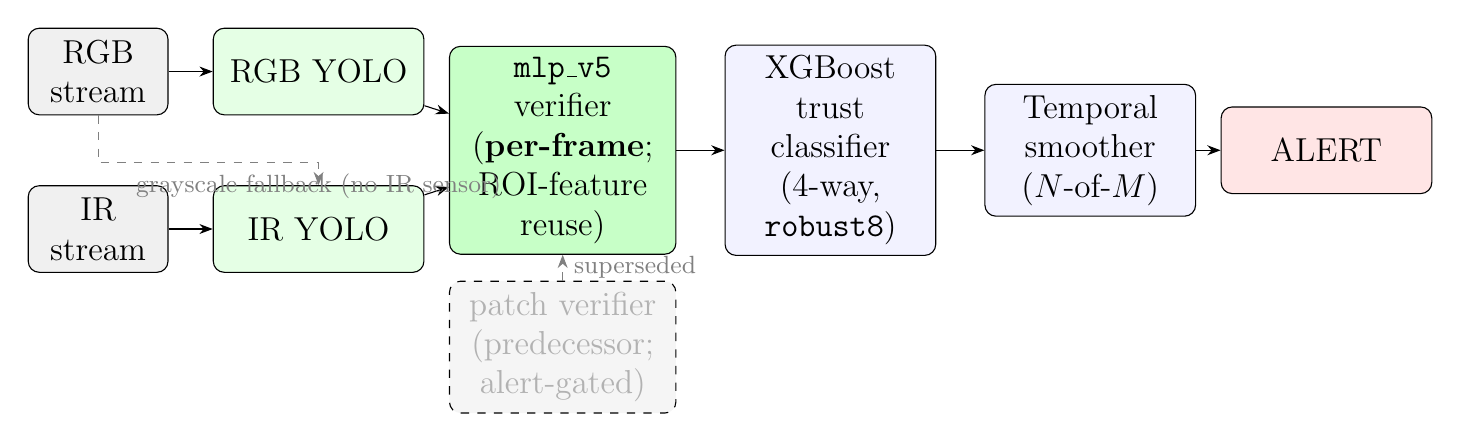
\begin{tikzpicture}[>=Stealth, font=\small,
      box/.style={draw, rounded corners, align=center, minimum height=11mm, text width=24mm, fill=blue!5},
      det/.style={box, fill=green!10},
      ver/.style={box, fill=green!22, text width=26mm},
      io/.style={box, fill=gray!12, text width=15mm},
      old/.style={draw, dashed, rounded corners, align=center, minimum height=10mm, text width=26mm, fill=gray!8, text=gray!60}]
      \node[io]  (rgb)  at (0,1.0)   {RGB stream};
      \node[io]  (ir)   at (0,-1.0)  {IR stream};
      \node[det] (ry)   at (2.8,1.0) {RGB YOLO};
      \node[det] (iy)   at (2.8,-1.0){IR YOLO};
      \node[ver] (ver)  at (5.9,0)   {\texttt{mlp\_v5} verifier\\(\textbf{per-frame};\\ROI-feature reuse)};
      \node[box] (clf)  at (9.3,0)   {XGBoost trust\\classifier\\(4-way, \texttt{robust8})};
      \node[box] (temp) at (12.6,0)  {Temporal\\smoother\\($N$-of-$M$)};
      \node[box, fill=red!10] (alert) at (15.6,0) {ALERT};
      \node[old] (patch) at (5.9,-2.5) {patch verifier\\(predecessor; alert-gated)};
      \draw[->] (rgb)--(ry);   \draw[->] (ir)--(iy);
      \draw[->] (ry)--(ver);   \draw[->] (iy)--(ver);
      \draw[->] (ver)--(clf);  \draw[->] (clf)--(temp); \draw[->] (temp)--(alert);
      \draw[->, dashed, gray] (patch) -- node[right, font=\scriptsize, text=gray]{superseded} (ver);
      \draw[->, dashed, gray] (rgb.south) -- ($(rgb.south)+(0,-0.6)$) -| (iy.north)
            node[midway, below, font=\scriptsize, text=gray]{grayscale fallback (no IR sensor)};
    \end{tikzpicture}}
    \caption{Multi-stage drone detection pipeline. The production confuser verifier is the distilled \texttt{mlp\_v5}, which runs \textbf{per frame} because it reuses the detectors' already-computed ROI features rather than re-processing crops (\S\ref{sec:distill_verifier}; \textsc{Ledger}~v5-ship-per-frame). It supersedes the MobileNetV3 patch verifier (greyed), which was expensive enough that it had to be \emph{alert-gated} --- consulted only when the temporal smoother was about to fire (\S\ref{sec:alert_gate}).}
    \label{fig:pipeline}
\end{figure}

The headline numbers for the cascade are deferred to Chapter~\ref{ch:experiments}. The point to carry into the rest of this chapter is that the cascade's downstream stages contribute the majority of confuser suppression without retraining the detectors. This property is the consequence of three architectural choices: fail-open detection (\S\ref{sec:design_rationale}), trust-aware fusion (\S\ref{sec:trust_fusion}), and a downstream confuser verifier --- in production the per-frame distilled \texttt{mlp\_v5} (\S\ref{sec:distill_verifier}).

\paragraph{A note on the verifier across the evaluation chapters.} The production confuser verifier is the per-frame distilled \texttt{mlp\_v5} (RGB, \S\ref{sec:distill_verifier}) and its cross-modal counterpart \texttt{mlp\_v5\_ir\_aligned} (IR, \S\ref{sec:ir_xmodal_verifier}); both are implemented in the deployed \texttt{MLPVerifier} and are the recommended stack. The full-cascade \emph{experiments} reported in Chapter~\ref{ch:experiments} (the Svanstr\"om sweep of \S\ref{sec:cumulative} and the real-video cascade of \S\ref{sec:realvideo_cascade}) were run with the older MobileNetV3 patch verifier at the alert gate, which predates the distilled verifier; those numbers therefore characterise the cascade with its \emph{predecessor} verifier and are conservative with respect to the production stack. A full-pipeline re-evaluation with the per-frame \texttt{mlp\_v5} verifier in the alert-gate slot is a registered open item (\textsc{Ledger}~v5-ship-per-frame; placeholder, \S\ref{sec:realvideo_cascade}); the component-level evidence that \texttt{mlp\_v5} dominates the patch verifier on every confuser-rich surface is in \S\ref{sec:distill_verifier}.

\paragraph{Two-verifier fusion (trust-first).} With both RGB (\texttt{mlp\_v5}) and IR (\texttt{mlp\_v5\_ir\_aligned}) verifiers running per-frame, fusion is \emph{trust-first}: the trust classifier (\S\ref{sec:trust_fusion}) routes, then the trusted modality's verifier filters. \texttt{reject\_both} drops the frame; \texttt{trust\_rgb} keeps it only if the RGB verifier passes; \texttt{trust\_ir} keeps it only if the IR verifier passes; \texttt{trust\_both} is resolved per-modality (recall-first: the detection survives if either trusted verifier passes), with a cross-modal soft-weighted tie-break left as future work. The IR verifier can run always-on because the grayscale$\leftrightarrow$thermal alignment (\S\ref{sec:ir_xmodal_verifier}) makes it recall-safe rather than recall-eroding. This ordering is classifier-agnostic: it is unchanged whether the router is the shipped \texttt{robust8} (its \texttt{robust6} base, \S\ref{sec:feature_selection}) or the \texttt{sa32} comparison classifier.
% [source: ledger=dual-verifier-fusion-rule; eval=clf_own_holdout; run=eval/overnight_ablation.py; config=clf_own_holdout]

\section{Design Rationale: Fail-Open}
\label{sec:design_rationale}

The cascade's central design principle is asymmetric recoverability. This is a property of the \emph{detector choice and cascade ordering}, not of any single downstream stage --- in particular it should not be conflated with the alert-gated patch verifier (\S\ref{sec:alert_gate}), which is one filtering stage operating \emph{within} a fail-open cascade. A confuser false positive raised by the detector can be vetoed by a downstream stage, but a drone that the detector missed cannot be re-introduced by any downstream stage. The cascade therefore ``fails open'' at the detector: when the detector is uncertain it keeps the detection and defers suppression to later stages, rather than suppressing early at the cost of unrecoverable misses. Both detectors are trained with confuser negatives (\S\ref{sec:rgb_three_variants}, \S\ref{sec:ir_detector}), but training-time mining does not eliminate all categories: in particular, bird hallucination is irreducible at the RGB detector stage at small drone sizes (\S\ref{sec:lit_fusion}). The cascade is built around that residual, training-time mining recovers what it can; the downstream stages catch what is left, especially on bird-on-sky and OOD imagery.

The cost is real and is visible in the same evaluation as the win. The three RGB-detector variants (Table~\ref{tab:rgb_comparison}; \textsc{Ledger}~\S3.1) trace the lever: the baseline reaches drone $R=0.961$ on Svanstr\"om with a 94.4\% bird-frame fire rate; \texttt{retrained\_v2} cuts bird-frame fire to 3.4\% but drops drone recall to $R=0.306$. The collapse is Svanstr\"om-specific (on Roboflow OOD drones the same \texttt{retrained\_v2} retains $R=0.726$ vs baseline $R=0.746$), but for any deployment that must catch small drones it is disqualifying.
% [source: ledger=retrainedv2-recall-collapse; eval=rgb_svan_retrainedv2; run=eval/diagnose_failures_all.py; cache=eval/results/_failure_diagnosis/svanstrom_1280_by_category.csv; config=svan_iop_1280]

The cascade takes the recall-preserving baseline and uses the downstream stages to reduce OOD confuser fire rate. The in-distribution cost is real but operating-point-dependent. On the OOD confuser zoo, with the open-world fallback classifier \texttt{fusion\_no\_fn\_v1.1}, the classifier carries the bulk of the suppression ($52.1\% \to 1.6\%$) and the patch verifier roughly halves the residual ($1.6\% \to 0.8\%$); with the sa32 comparison classifier on the same zoo the suppression is shallower but still substantial ($52.1\% \to 20.5\% \to 10.3\%$) (\textsc{Ledger}~\S7). On Svanstr\"om paired drones the same stages drop trust-aware $F1$ from 0.950 (S1) to 0.914 (S2) to 0.868 at \texttt{patch\_thr}$=$0.5, recovering to 0.895 at \texttt{patch\_thr}$=$0.9. On the real-video diagnostic, however, the full-cascade experiment (run with the \texttt{sa32} comparison classifier and the predecessor patch verifier, $\mathtt{patch\_thr}=0.7$; the production \texttt{robust8}/\texttt{mlp\_v5} re-run is a registered open item, \S\ref{sec:realvideo_cascade}) does not pay any in-distribution drone-F1 cost: temporal smoothing on three-frame windows recovers per-frame misses, and the full cascade lifts baseline-RGB drone segment $F1$ from $0.760$ (RGB alone) to $0.826$ (cascade) while cutting confuser segment FPR from $0.512$ to $0.162$ ($-68\%$) (\S\ref{sec:realvideo_cascade}, \textsc{Ledger}~\S9.5). The cascade is therefore not an unconditional precision boost on Svanstr\"om-paired data; but on real video with the production classifier it is monotonically better than the RGB stage alone. The exchange between in-distribution $F1$ and OOD safety is jointly driven by the classifier and the evaluation surface (RQ2; \S\ref{sec:rq_answers}), not by the cascade structure itself.
% [source: ledger=cascade-confuser-collapse; eval=clfzoo_fnfn; run=eval/cumulative_halluc.py; cache=eval/results/_cumulative_halluc/confuser_fusion_no_fn_model_v1.1/summary.json; config=confuser_zoo_1280]

\section{Trust-Aware Fusion}
\label{sec:trust_fusion}

The fusion stage is a learned per-frame decision rather than a fixed vote. The classifier outputs one of four labels:

\begin{itemize}
    \item \textbf{\texttt{reject\_both}}, neither modality's detection is trustworthy (likely a confuser).
    \item \textbf{\texttt{trust\_rgb}}, only RGB is reliable for this frame.
    \item \textbf{\texttt{trust\_ir}}, only IR is reliable for this frame.
    \item \textbf{\texttt{trust\_both}}, both modalities agree and are trustworthy.
\end{itemize}

The 4-way formulation captures \emph{when} each modality is reliable. The data-supported asymmetry is not primarily a lighting one. On Svanstr\"om paired data the IR detector ($P=0.950, R=0.973, F1=0.961$) is in fact stronger than the RGB detector at \texttt{imgsz=1280} (drone $F1=0.950$, from $P=0.940$/$R=0.961$, Table~\ref{tab:rgb_comparison}) on drones. On the real-video diagnostic the IR detector fed grayscale-RGB sits on the joint $(F1, \mathrm{FPPI})$ Pareto frontier --- $3.2\times$ lower aggregate confuser FPPI than the RGB baseline ($0.158$ vs $0.512$) at $-12.4$~pp drone F1 (\S\ref{sec:realvideo}). The asymmetry the classifier exploits is therefore: \emph{the two detectors hallucinate on different scenes}. Visual confusers (birds at small scale, helicopters against sky) fool the RGB detector more reliably than the IR detector; thermally degraded conditions (low contrast, hot backgrounds) fool the IR detector more reliably than RGB. Night-vs-day is a special case of the same axis (RGB loses signal at night, IR does not). A per-frame classifier can pick the modality whose failure profile is least active in the current scene; a fixed-weight rule cannot.
% [source: ledger=no-pareto-dominance-video; eval=vid_drone_ir_gray; run=eval/eval_video_tests.py; config=video_drone_iop]

The feature set varies by classifier variant; the production stack uses the six free, leakage-aware features of \texttt{robust6} (per-modality detection confidence and box geometry; \S\ref{sec:feature_selection}), which statistically supersede the 32-feature \texttt{scene\_aware\_v3more\_32feat} (\texttt{sa32}) that served as the working pick through the real-video classifier comparison (\S\ref{sec:realvideo_classifier}). Two hand-engineered alternatives are retained for comparison and for non-default deployments: \texttt{control\_v3more\_40feat} for confuser-dense surfaces where reducing fire rate matters more than drone recall, and \texttt{fusion\_no\_fn\_v1.1} for unknown-distribution open-world deployment (\S\ref{sec:classifier_variants}).
% [source: ledger=robust6-production-viable,ft4-lean-trust-classifier; eval=clf_own_holdout; run=classifier/train_lean_ft4.py; cache=docs/analysis/2026-05-31_ft4_lean_trust_classifier.md; config=clf_own_holdout] Detector signals (in particular the presence of an IR detection) are among the most informative features in every variant, but the exact ranking is variant-specific and is reported per classifier rather than asserted as a global ``IR detection contributes $X\%$'' figure.

\section{Alert-Gate Cascade}
\label{sec:alert_gate}

This section describes the deployment of the MobileNetV3 \emph{patch} verifier, the predecessor that the per-frame \texttt{mlp\_v5} verifier (\S\ref{sec:distill_verifier}) now supersedes. Alert-gating was forced by the patch verifier's cost --- a second CNN over crop pixels --- and is no longer needed once the verifier reuses the detectors' features; it is retained here because it is the design under which the patch verifier was audited.

The patch verifier is positioned at the \emph{alert gate}: it is consulted only when the temporal smoother is about to emit an alert (i.e., when the rolling per-frame decision window is about to complete an alert-triggering majority). Two alternative cascades were considered and rejected:

\begin{itemize}
    \item \textbf{\texttt{filter\_then\_classifier}}, run the patch verifier on every detection \emph{before} the trust classifier. Per-frame patch filtering cost $\approx 1$~pp Svanstr\"om F1 by vetoing marginal drone TPs whose patch probability fell into the soft middle of the verifier's distribution (\textsc{Ledger}~\S1, \texttt{D\_cascade}).
    \item \textbf{\texttt{classifier\_then\_filter}}, run the patch verifier on every frame after the classifier accepts. Same problem at smaller magnitude.
\end{itemize}

Both are implemented in \texttt{eval/eval\_pipeline.py} but neither matches production. The production cascade is \texttt{alert\_gate\_only}, implemented in \texttt{eval/eval\_video\_temporal.py} and in the PySide GUI's \texttt{should\_suppress\_alert(\dots)} (\texttt{ir\_gui/pyside\_engine.py}). The verifier's CNN runs only at the moment a temporal window resolves into an alert, so the per-frame latency cost of the verifier is zero on the overwhelming majority of frames.

\section{Temporal Smoother}
\label{sec:temporal}

The temporal smoother is an $N$-of-$M$ sliding-window aggregator with configurable cooldown. An alert fires only when the trust classifier's per-frame decision has been positive on at least $N$ of the last $M$ frames; after firing, a cooldown suppresses immediate re-fires from the same track. The smoother absorbs isolated firings characteristic of birds and aircraft transiting the field of view.

The same temporal state drives a \emph{ROI fallback} in the PySide engine (\texttt{\_run\_with\_roi}). When the full-frame YOLO returns nothing and a recent track is still alive, YOLO is re-run on an expanded crop around the previous box at reduced confidence. This is a GUI-only feature, and the frame-mode evaluation harness does not use it; it accounts for part of the GUI-versus-eval performance gap on small distant drones. The GUI maintains tracks and renders a path image, but does not yet classify on track-level features (flight dynamics); that is the most promising single direction for future work.

Frame-independent evaluation (the standard scoring mode in \texttt{eval/cumulative\_halluc.py}) deliberately omits the temporal smoother so that per-stage contributions can be measured cleanly. The headline numbers in this chapter are therefore lower bounds on the deployed system's confuser rejection; the temporal smoother contributes additional rejection in real video that is not credited to any cascade stage in the reported metrics.

\begin{figure}[htbp]
    \centering
    \fbox{\parbox{0.9\textwidth}{\centering\vspace{2cm}
        \textbf{[PLACEHOLDER: Fig 3.2 --- PySide6 deployment GUI]} Annotated screenshot of the deployed GUI: dual-modality view (RGB + IR side by side), per-frame trust-label readout, sliding temporal window indicator, alert banner, ROI fallback crop inset, drone-path overlay across recent frames, threshold sliders for RGB / IR / patch.
    \vspace{2cm}}}
    \caption{PySide6 deployment GUI. The temporal smoother's state, the trust classifier's per-frame decision, and the ROI fallback crop are all surfaced for the human operator; the patch verifier runs silently at the alert gate.}
    \label{fig:pyside_gui}
\end{figure}

\section{Resolution Dependency}
\label{sec:resolution_arch}

Resolution is the single largest hyperparameter affecting small-drone recall and is treated as a first-class architectural decision rather than a tuning knob. Svanstr\"om's native resolution is $640\times 512$; at \texttt{imgsz=1280} the baseline RGB detector reaches $R=0.961$ on Svanstr\"om drones, whereas at \texttt{imgsz=640} small drones fall below the resolvable floor --- the \texttt{retrained\_v2} variant measured at that size collapses to $R=0.072$, and the baseline's own \texttt{imgsz=640} run is pending (\textsc{Ledger}~\S3.1, \S10). Anti-UAV imagery, at $1920\times 1080$ native resolution, saturates at the default \texttt{imgsz=640} because drones already span enough pixels at the input. All Svanstr\"om RGB evaluation in this thesis therefore uses \texttt{imgsz=1280}. Selcom CCTV imagery (\S\ref{sec:selcom}) is a third regime: clutter is the binding constraint there, not pixel size, and the imgsz sweep documented in \texttt{docs/analysis/2026-05-16\_rgb\_camera\_spec\_and\_fault\_profile.md} identifies $\mathtt{imgsz}=960$ as the F1-optimal production setting for that camera.
% [source: ledger=selcom-imgsz-win; eval=rgb_svan_baseline; run=eval/diagnose_failures.py; cache=eval/results/_failure_diagnosis/svanstrom_1280_by_category.csv; config=svan_iop_1280]

\begin{figure}[htbp]
    \centering
    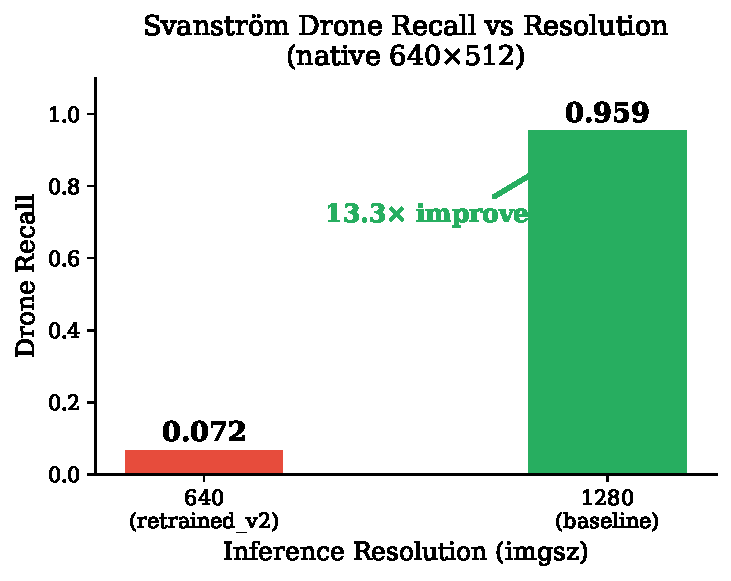
\includegraphics[width=0.85\textwidth]{fig6_6_resolution}
    \caption{Inference-resolution dependency of Svanstr\"om drone recall. At \texttt{imgsz=1280} the baseline detector reaches $R=0.961$; the \texttt{imgsz=640} floor is illustrated with \texttt{retrained\_v2} ($R=0.072$), the only variant measured at that size --- the baseline's own \texttt{imgsz=640} run is pending (\S\ref{sec:resolution_arch}), so the two endpoints are different variants and the curve is indicative, not a single-model sweep. Source: \textsc{Ledger}~\S3.1, \S10.}
    % [source: ledger=retrainedv2-recall-collapse; eval=rgb_svan_baseline; run=eval/diagnose_failures.py; cache=eval/results/_failure_diagnosis/svanstrom_1280_by_category.csv; config=svan_iop_1280]
    \label{fig:resolution}
\end{figure}

\section{RGB Drone Detector}
\label{sec:rgb_detector}

The RGB detector is a YOLOv26n (nano) single-class detector. The nano variant is the smallest weight class in the Ultralytics family. The training corpus combines Anti-UAV RGB frames~\cite{jiang2021antiuav}, Roboflow community drone datasets, and a drone-vs-bird subset that supplies bird frames as deliberate confuser negatives. Svanstr\"om imagery is held out from training so that Svanstr\"om remains a genuine OOD evaluation for the detector. Across the three variants below, the question explored is how much additional confuser-specific training data is the right amount to add on top of this baseline corpus.

\subsection{Three Training Stances}
\label{sec:rgb_three_variants}

Three RGB-detector variants were trained and compared. They represent three operating points on the recall--hallucination axis, and the comparison is the empirical basis for the cascade's design rationale (\S\ref{sec:design_rationale}).

\begin{enumerate}
    \item \textbf{Baseline} (\texttt{Yolo26n\_trained}). Trained on the composite drone corpus, which includes the drone-vs-bird subset as deliberate confuser negatives but does not include Svanstr\"om-style confuser splits as explicit negatives. On Svanstr\"om@1280 it reaches $P=0.940, R=0.961$ on drones (\textsc{Ledger}~\S3.1).
    % [source: ledger=retrainedv2-recall-collapse; eval=rgb_svan_baseline; run=eval/diagnose_failures.py; cache=eval/results/_failure_diagnosis/svanstrom_1280_by_category.csv; config=svan_iop_1280]
    \item \textbf{\texttt{hardneg\_v3more}} (\texttt{Yolo26n\_hardneg\_v3more}). Same backbone, retrained with the Svanstr\"om bird/airplane/helicopter confuser splits supplied as additional negatives. Drone $P=0.941, R=0.950$; helicopter fire rate drops from 66.2\% to 41.9\%, airplane fire rate from 74.6\% to 64.7\%, but bird fire rate is essentially unchanged at 94.2\% (\textsc{Ledger}~\S3.1).
    % [source: ledger=retrainedv2-recall-collapse; eval=rgb_svan_baseline; run=eval/diagnose_failures.py; cache=eval/results/_failure_diagnosis/svanstrom_1280_by_category.csv; config=svan_iop_1280]
    \item \textbf{\texttt{retrained\_v2}} (\texttt{Yolo26n\_retrained\_v2}). Aggressive retraining with heavy confuser augmentation. Bird fire rate collapses to 3.4\% but Svanstr\"om drone recall collapses to $R=0.306$ at the same operating threshold. The collapse is Svanstr\"om-specific: on Roboflow OOD drone splits the same weights retain $R=0.726$ (\textsc{Ledger}~\S8.1).
    % [source: ledger=selcom-ood-confuser-damage; eval=rob_rgb_baseline; run=eval/run_roboflow_eval.py; config=roboflow_rgb_drone_640]
\end{enumerate}

The pattern is class-specific. Adding Svanstr\"om confuser negatives works for helicopters (large change), works partially for airplanes (moderate change), and does not work for birds at small scale (no change). Birds and small drones share too much low-level structure for the YOLO feature extractor to discriminate them reliably without an unacceptable recall cost. The cascade is the response specifically to the bird case; the helicopter and airplane suppressions are achievable at the detector stage and are visible in the \texttt{hardneg\_v3more} row.

\begin{table}[htbp]
    \centering
    \caption{RGB variants on Svanstr\"om @ \texttt{imgsz=1280} (IoP@0.5, drone class). Aggressive retraining destroys recall on small Svanstr\"om drones while leaving Roboflow OOD performance comparable. Source: \textsc{Ledger}~\S3.1.}
    \label{tab:rgb_comparison}
    \begin{tabular}{lccccc}
        \toprule
        Model & Drone $P$ & Drone $R$ & Bird halluc & Airplane halluc & Heli halluc \\
        \midrule
        baseline           & 0.940 & \textbf{0.961} & 94.4\% & 74.6\% & 66.2\% \\
        \texttt{hardneg\_v3more}  & 0.941 & 0.950 & 94.2\% & 64.7\% & 41.9\% \\
        \texttt{retrained\_v2}    & 0.943 & 0.306 & \textbf{3.4\%}  & \textbf{5.6\%}  & \textbf{4.5\%}  \\
        \bottomrule
    \end{tabular}
\end{table}

\begin{figure}[htbp]
    \centering
    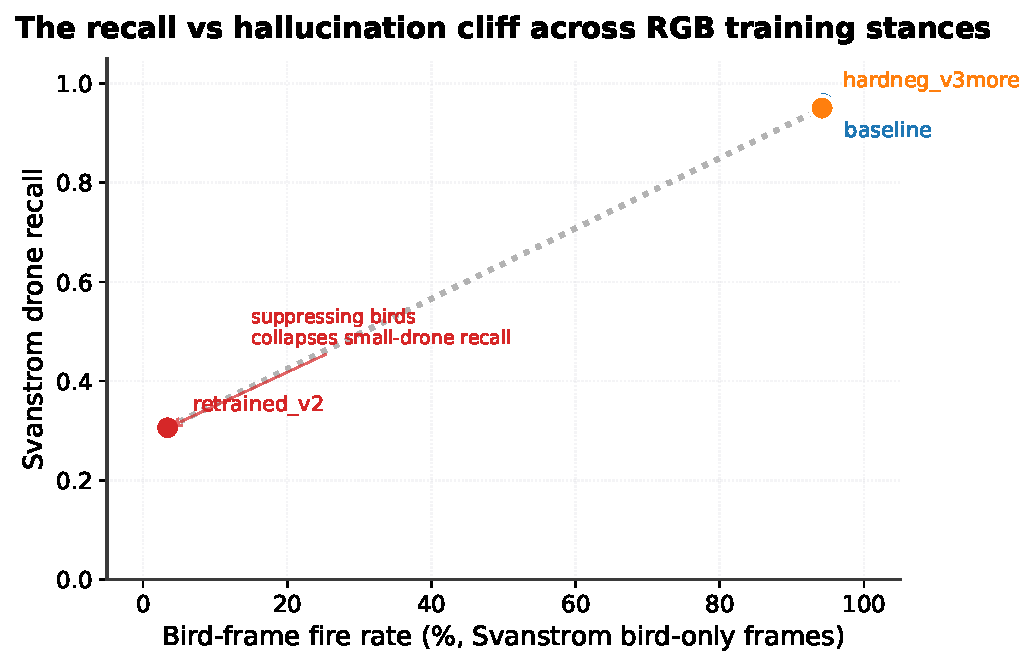
\includegraphics[width=0.7\textwidth]{fig8_rgb_threestance}
    \caption{The recall--hallucination cliff across the three RGB training stances. Suppressing bird-frame fire from $94.4\%$ (baseline) to $3.4\%$ (\texttt{retrained\_v2}) collapses Svanstr\"om drone recall from $0.961$ to $0.306$; \texttt{hardneg\_v3more} barely moves bird fire ($94.2\%$). The cascade exists to recover the bird suppression without paying the recall cost. Source: \textsc{Ledger}~\S3.1 (Table~\ref{tab:rgb_comparison}).}
    % [source: ledger=retrainedv2-recall-collapse; eval=rgb_svan_baseline,rgb_svan_retrainedv2; run=eval/diagnose_failures_all.py; cache=eval/results/_failure_diagnosis/svanstrom_1280_by_category.csv; config=svan_iop_1280]
    \label{fig:rgb_threestance}
\end{figure}

The same comparison at \texttt{imgsz=640} on Svanstr\"om was run for \texttt{retrained\_v2} (\textsc{Ledger}~\S3.1, $P=0.837, R=0.072$) and confirms that the \texttt{imgsz=640} regime is unusable for Svanstr\"om regardless of variant; the equivalent \texttt{imgsz=640} runs for the baseline and \texttt{hardneg\_v3more} are flagged as TBD (\textsc{Ledger}~\S10, placeholder).
% [source: ledger=retrainedv2-recall-collapse; eval=rgb_svan_baseline; run=eval/diagnose_failures.py; cache=eval/results/_failure_diagnosis/svanstrom_1280_by_category.csv; config=svan_iop_1280]

\subsection{SelCom CCTV Fine-Tune}
\label{sec:selcom_finetune}

A separate fine-tune line targets a fixed-camera 7~Mbps HEVC CCTV stream from the deployment partner SelCom. The fine-tune is performed on top of the \emph{baseline} \texttt{Yolo26n\_trained} weights (not \texttt{retrained\_v2}); this matters downstream because the trust classifiers were calibrated against baseline-family RGB confidence distributions (\S\ref{sec:classifier_variants}), so the selcom-fine-tuned weights remain compatible with the deployed cascade without a classifier swap. The selcom imagery itself is OOD for the baseline: drones are small (median $\sqrt{\text{area}} \approx 37$~px in the source frame, $\sim 12$~px at \texttt{imgsz=640}, $\sim 24$~px at \texttt{imgsz=1280}) and blend into urban clutter. Two mixed-training fine-tunes (80\% general RGB + 20\% selcom; pure-selcom val split, seed 0) were evaluated at IoP@0.5, conf$=$0.25 on \texttt{selcom\_mixed\_ft2\_val} (311 images, 295 GT boxes):
% [source: ledger=selcom-imgsz-win; eval=selcom_ft2_1280; run=RGB model/finetune_selcom.py; cache=runs/rgb_finetune_eval/Yolo26n_selcom_mixed_ft2_1280/comparison.json; config=selcom_iop_1280]

\begin{table}[htbp]
    \centering
    \caption{SelCom CCTV fine-tune; IoP@0.5, conf=0.25, val split 311~imgs / 295~GT. The production CCTV stack uses \texttt{Yolo26n\_selcom\_mixed\_ft2\_1280}. Source: \textsc{Ledger}~\S3.4.}
    \label{tab:selcom}
    \begin{tabular}{lcccccc}
        \toprule
        Model & imgsz & TP & FP & FN & $P$ & $R$ \\
        \midrule
        baseline (\texttt{Yolo26n\_trained})        & 640  &   2 &  6 & 293 & 0.250 & 0.007 \\
        baseline                                    & 1280 &  26 & 37 & 269 & 0.413 & 0.088 \\
        \texttt{Yolo26n\_selcom\_mixed\_ft2}        & 640  &  72 & 50 & 223 & 0.590 & 0.244 \\
        \textbf{\texttt{Yolo26n\_selcom\_mixed\_ft2\_1280}} & \textbf{1280} & \textbf{138} & \textbf{43} & \textbf{157} & \textbf{0.762} & \textbf{0.468} \\
        \bottomrule
    \end{tabular}
\end{table}

The \texttt{ft2\_1280} weights both double selcom recall vs \texttt{ft2@640} (0.244 $\to$ 0.468) \emph{and} raise precision (0.590 $\to$ 0.762). The regression check on the standard RGB dataset is within $-0.008$ F1 of baseline at \texttt{imgsz=1280} (\textsc{Ledger}~\S3.4, dataset\_rgb pair). A preprocessing sweep run on selcom established that no OpenCV preprocessing variant (denoise, CLAHE, sharpen, contrast) improves selcom detection independently of fine-tuning and \texttt{imgsz}; the relevant levers are training data and resolution, not pre-inference filtering (\texttt{runs/preprocess\_sweep/REPORT.md}; \textsc{Ledger}~\S3.4 notes).
% [source: ledger=selcom-imgsz-win; eval=selcom_ft2_1280; run=RGB model/finetune_selcom.py; cache=runs/rgb_finetune_eval/Yolo26n_selcom_mixed_ft2_1280/comparison.json; config=selcom_iop_1280]

The imgsz sweep on selcom (4~models $\times$ 4~sizes $\times$ 3~datasets, \texttt{docs/analysis/2026-05-16\_rgb\_camera\_spec\_and\_fault\_profile.md}) further identifies $\mathtt{imgsz}=960$ as the F1-optimal CCTV setting: clutter is the binding constraint on selcom, not pixel size, and very high \texttt{imgsz} starts to amplify clutter-driven FPs faster than it improves drone recall.

\section{IR Drone Detector}
\label{sec:ir_detector}

The IR detector uses the same YOLOv26n architecture as the RGB detector, finetuned on iteratively curated thermal data (\S\ref{sec:hitl_ir}). Its training corpus includes bird, airplane, and helicopter thermal frames as hard negatives, fed into the dataset across HITL revisions whenever the previous IR detector hallucinated on a confuser scene (\S\ref{sec:hitl_ir}). The production weights (\texttt{runs/corrective\_finetune/finetune\_v3b/weights/best.pt}, hereafter \texttt{v3b}) are a 2-epoch corrective fine-tune on top of the \texttt{Final} checkpoint and address specific deployment-time failure modes. The full evolution trace across six numbered revisions --- including the V5 regression and its recovery --- is documented as a case study in Chapter~\ref{ch:hitl} (\S\ref{sec:ir_evolution}).

\subsection{IR Detector on Svanstr\"om and Anti-UAV}

The same \texttt{v3b} weights were evaluated on the two public benchmarks under the May~10 ablation matrix (\textsc{Ledger}~\S4). On Svanstr\"om at its native \texttt{imgsz=640}, IR-only reaches $P=0.950, R=0.973, \text{F1}=0.961$ (TP$=$2234, FP$=$117, FN$=$63). On Anti-UAV (May~10 default), IR-only reaches $P=0.987, R=0.945, \text{F1}=0.9654$. The IR detector is the stronger single-modality detector on both benchmarks; the role of the trust classifier is not to compensate for a weak modality but to choose between two competent modalities with different confuser-hallucination profiles (\S\ref{sec:trust_fusion}). The IR detector's brittleness lives elsewhere (on OOD thermal imagery (\S\ref{sec:roboflow}, $R=0.519$ on \texttt{ir\_mixed\_cbam}, $R=0.264$ on \texttt{ir\_drone\_night})) which is what motivates retaining the RGB detector at all.
% [source: ledger=prov-may10-imgsz; eval=ir_v3b_svan640_may10; run=(May-10 ablation matrix); cache=eval/results/_ablation/2026-05-10T16-08-14/master.csv; config=svan_iop_640_may10]

\subsection{Grayscale-RGB Operating Mode}
\label{sec:ir_grayscale_mode}

The deployed PySide GUI exposes a \emph{grayscale-RGB} operating mode for the IR detector (\texttt{\_infer\_grayscale} in \texttt{ir\_gui/pyside\_engine.py}). When no thermal camera is on hand, the GUI converts the RGB stream to single-channel grayscale via \texttt{cvtColor(BGR2GRAY)}, replicates to three channels, and feeds the result to the IR detector at its native \texttt{imgsz=640}. The mode existed because thermal sensors are expensive and not always available on the deployment platforms the system targets; without it, an RGB-only camera setup would lose the IR detection channel entirely.

What was not predicted at design time is how strongly the IR detector transfers across this modality gap; on the real-video diagnostic the grayscale fallback sits on the joint drone-$F1$ / confuser-FPPI Pareto frontier and ties the RGB baseline on the hardest bird-cluttered clip while having never seen visible-light data in training. The full quantification, mechanism, and limits are deferred to \S\ref{sec:grayscale} (and the Pareto reading to \S\ref{sec:realvideo}); the relevant point for component design is that the GUI fallback is, on some scenes, on par with the best visible-light detector, not a strict degradation mode.

\subsection{Cross-Modal Feature Alignment: a Thermal Verifier from Grayscale Confusers}
\label{sec:ir_xmodal_verifier}

The same grayscale-RGB mode underwrites a second, more consequential result: it dissolves the data-scarcity blocker that had previously kept any per-frame IR confuser verifier out of the production stack. The argument has two feature-space steps, both measured with the Model MRI tool (\S\ref{sec:model_mri}).

\emph{First, the confuser-rejection signal already lives inside the IR detector.} An MRI of the \texttt{v3b} fused \texttt{p3}+\texttt{p5} ROI features (517-D), over $14{,}697$ drone and $1{,}386$ confuser detections mined across IR surfaces, shows the two classes are almost linearly separable: a single linear discriminant reaches $0.981$ train accuracy (Figure~\ref{fig:ir_v3b_lda}a) and the strongest single neuron --- a \texttt{p5} channel --- carries an ANOVA $F=5{,}370$ (a near-binary ``is-this-a-drone'' switch; Figure~\ref{fig:ir_v3b_lda}b), against a raw detector hallucination rate of only $1.8\%$/image; a linear probe projects an $89\%$ false-positive cut at a $10\%$ recall cost. As on the RGB side (\S\ref{sec:distill_verifier}), a lightweight MLP can read this signal --- the IR detector does not need retraining.
% [source: ledger=ir-features-separable; eval=none (MRI run); run=mri/cli.py; cache=mri/results/ir_v3b_report; config=ir_v3b]

\begin{figure}[htbp]
    \centering
    \begin{subfigure}{0.6\textwidth}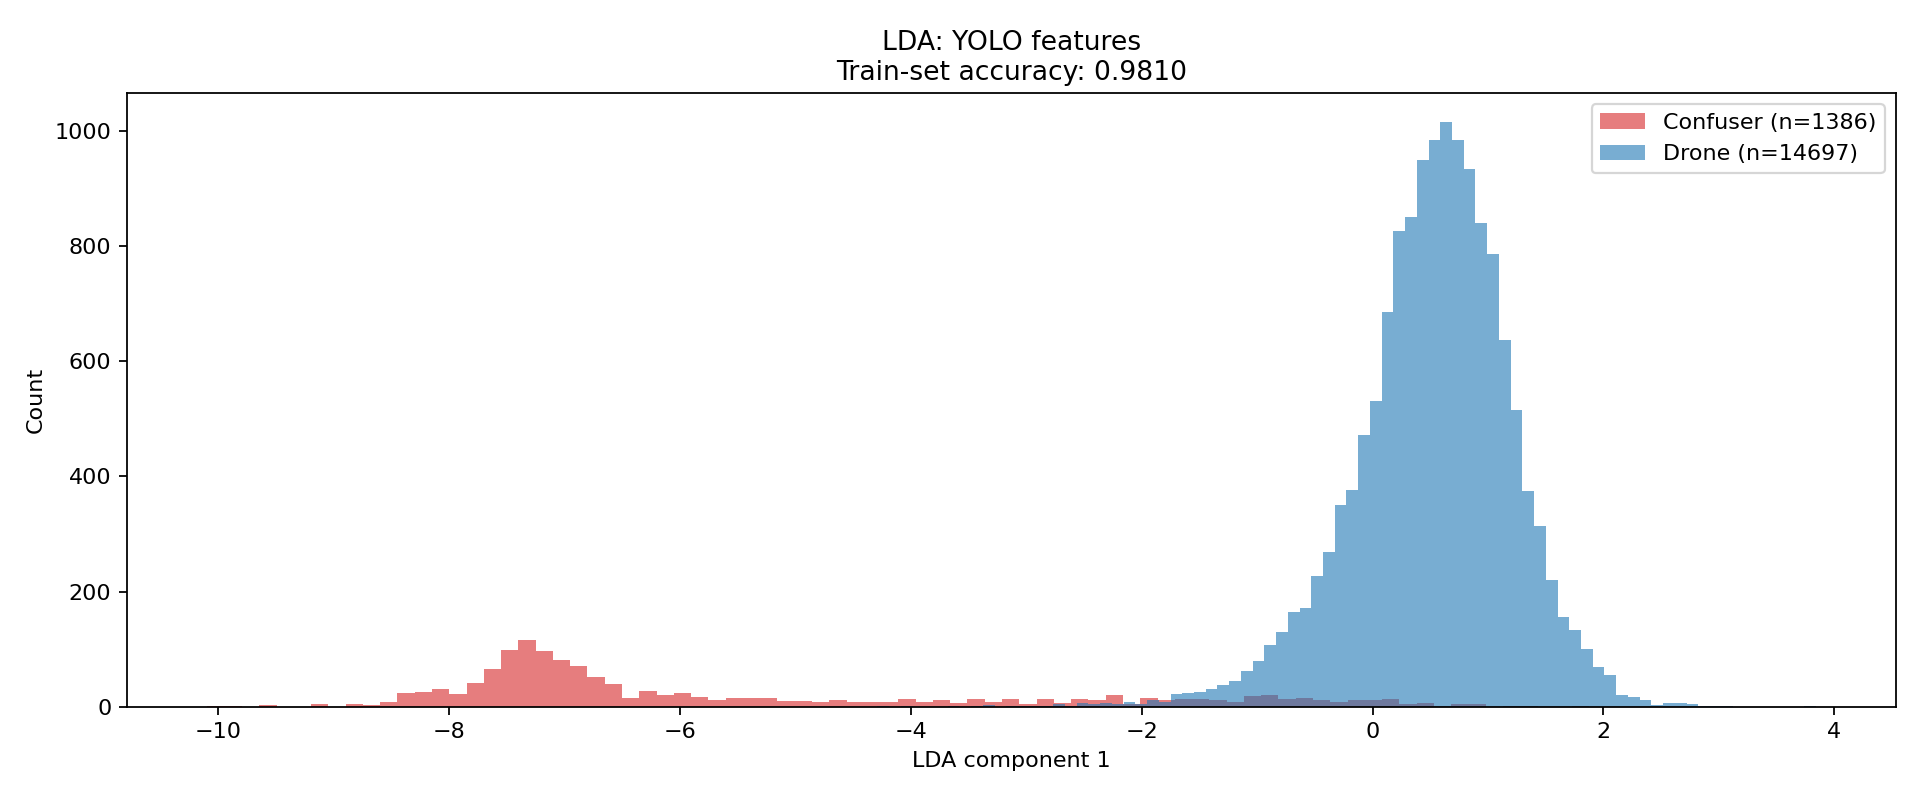
\includegraphics[width=\textwidth]{fig9_ir_v3b_lda}\caption{}\end{subfigure}
    \begin{subfigure}{0.39\textwidth}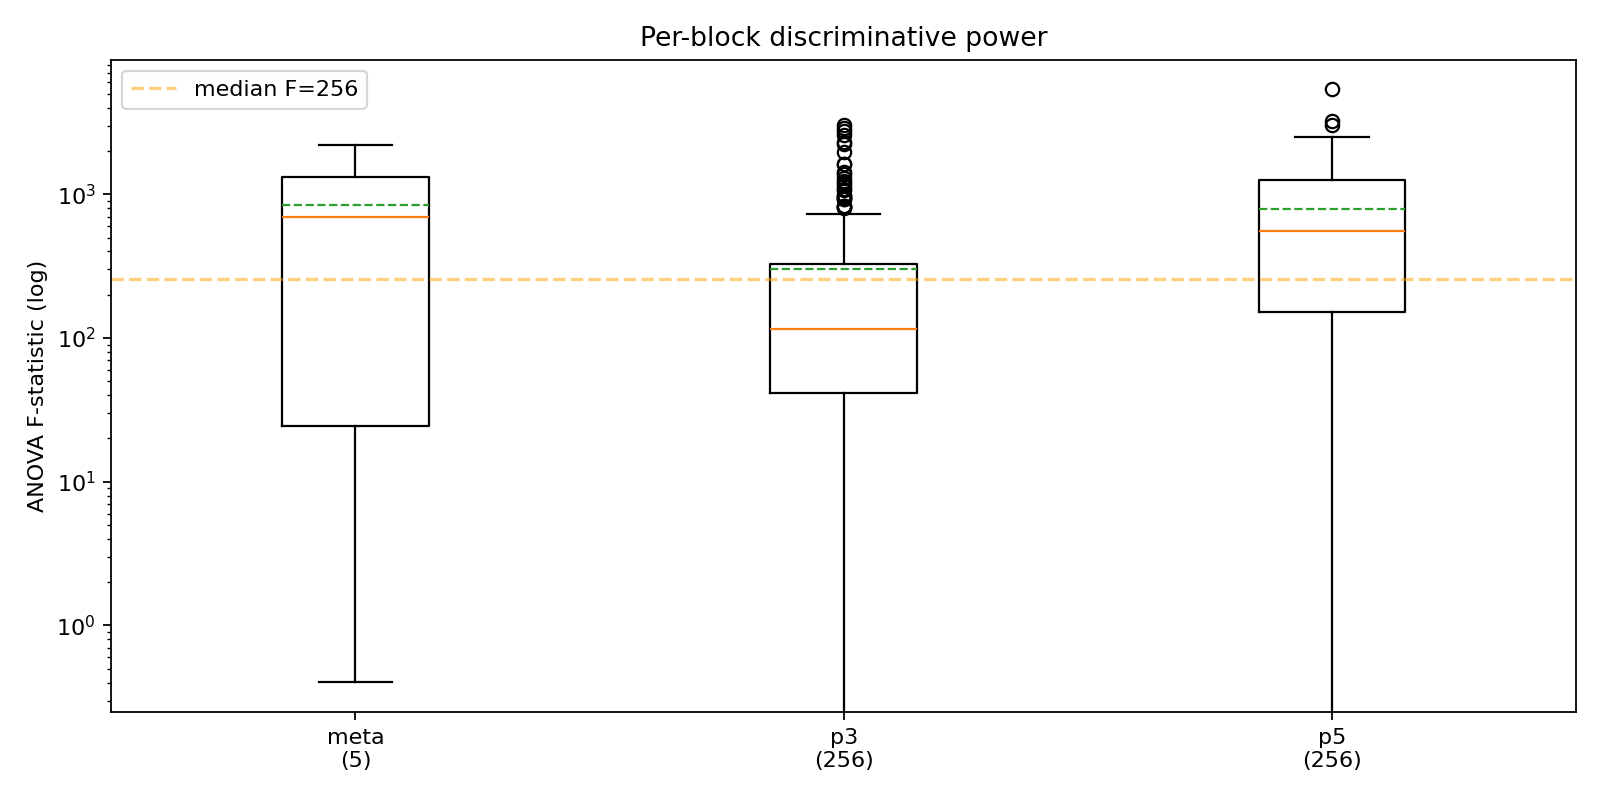
\includegraphics[width=\textwidth]{fig9_ir_v3b_anova}\caption{}\end{subfigure}
    \caption{Model MRI of the IR detector (\texttt{v3b}) fused \texttt{p3}+\texttt{p5} ROI features. (a) The linear-discriminant projection separates drones (green) and confusers (red) into two cleanly resolved peaks ($0.981$ train separability). (b) Per-block ANOVA $F$: the discriminative signal is concentrated in a few \texttt{p5} channels (max $F=5{,}370$), not diffuse. The confuser-rejection signal is already present in the detector's own features. Source: \textsc{Ledger}~ir-features-separable.}
    % [source: ledger=ir-features-separable; eval=none (MRI run); run=mri/cli.py; cache=mri/results/ir_v3b_report; config=ir_v3b]
    \label{fig:ir_v3b_lda}
\end{figure}

The same MRI shows \emph{what} the verifier reads. Ranking the top-20 discriminative features by per-class z-score (Figure~\ref{fig:ir_v3b_heatmap}) puts \texttt{p5} semantic channels at the top and the detection-confidence scalar (\texttt{meta:conf}) far down the list. The verifier keys on the detector's spatial activations, not merely its score, which is why a $517$-feature near-linear boundary --- and not a confidence threshold --- is what separates thermal drones from confusers.
% [source: ledger=ir-features-separable; eval=none (MRI run); run=mri/cli.py; cache=mri/results/ir_v3b_report; config=ir_v3b]

\begin{figure}[htbp]
    \centering
    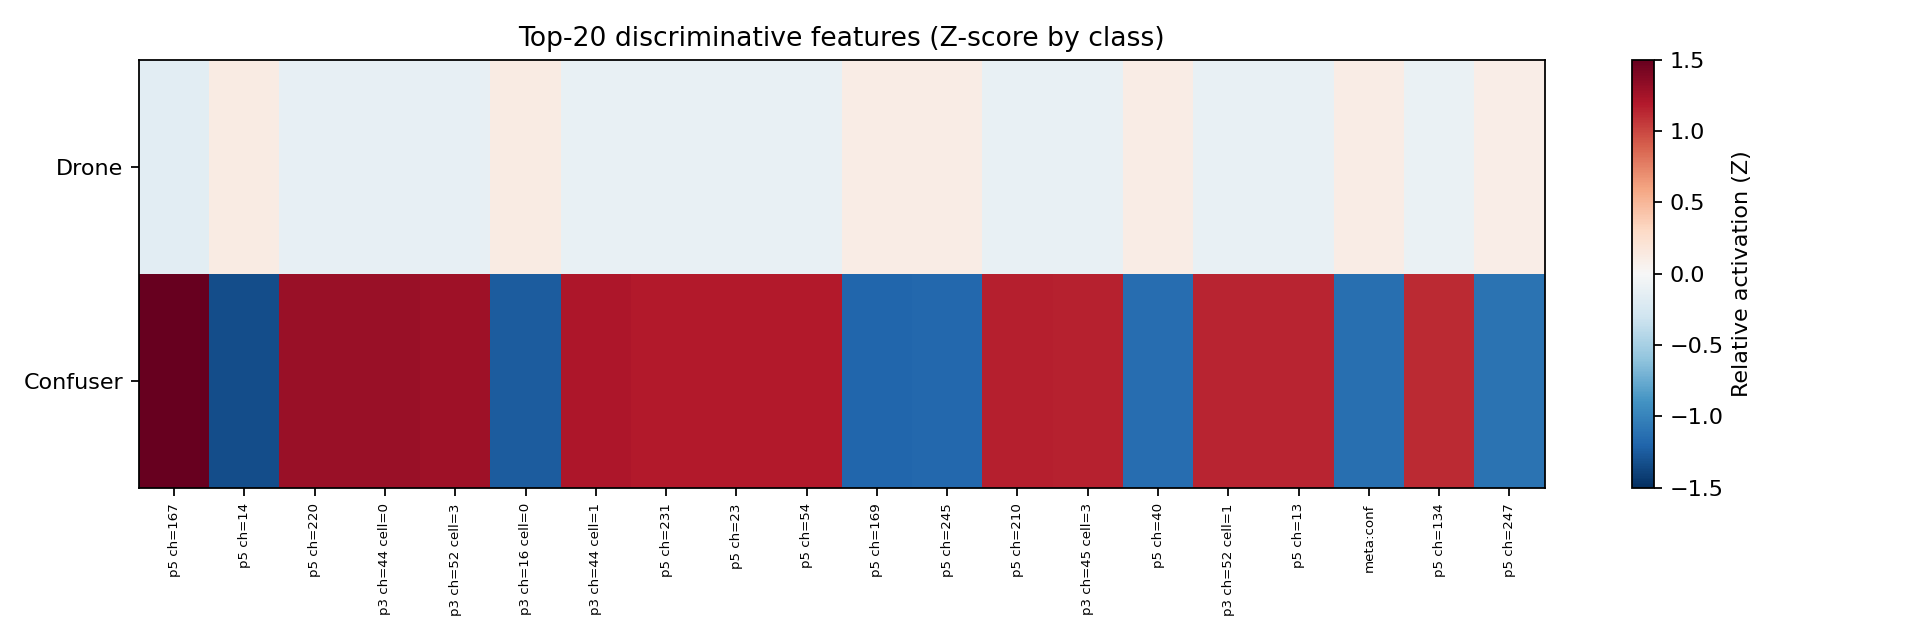
\includegraphics[width=0.95\textwidth]{fig9_ir_v3b_heatmap}
    \caption{Top-20 discriminative IR features (per-class z-score, drone vs.\ confuser) in the \texttt{v3b} detector. \texttt{p5} channels dominate; the detection-confidence scalar (\texttt{meta:conf}) is a minor contributor --- the thermal verifier reads the detector's semantic activations, not its score. Source: \textsc{Ledger}~ir-features-separable.}
    % [source: ledger=ir-features-separable; eval=none (MRI run); run=mri/cli.py; cache=mri/results/ir_v3b_report; config=ir_v3b]
    \label{fig:ir_v3b_heatmap}
\end{figure}

\paragraph{What the IR verifier sees, spatially.}
Rendering the IR detector's activations on real detections mirrors the RGB result (Figure~\ref{fig:mri_activation}): on a thermal drone the \texttt{p3} activation binds to the airframe and \texttt{p5} forms a centred semantic blob, whereas on a held-out CBAM confuser false-fire the same neurons scatter across background structure (Figure~\ref{fig:ir_mri_activation}). The thermal verifier reads the same kind of spatial signature its RGB counterpart does.
% [source: ledger=ir-features-separable; run=scripts/visualize_ir_activation.py; cache=docs/analysis/images/v5_ir_activation_drone_example.png; config=ir_v3b]

\begin{figure}[htbp]
    \centering
    \begin{subfigure}{\textwidth}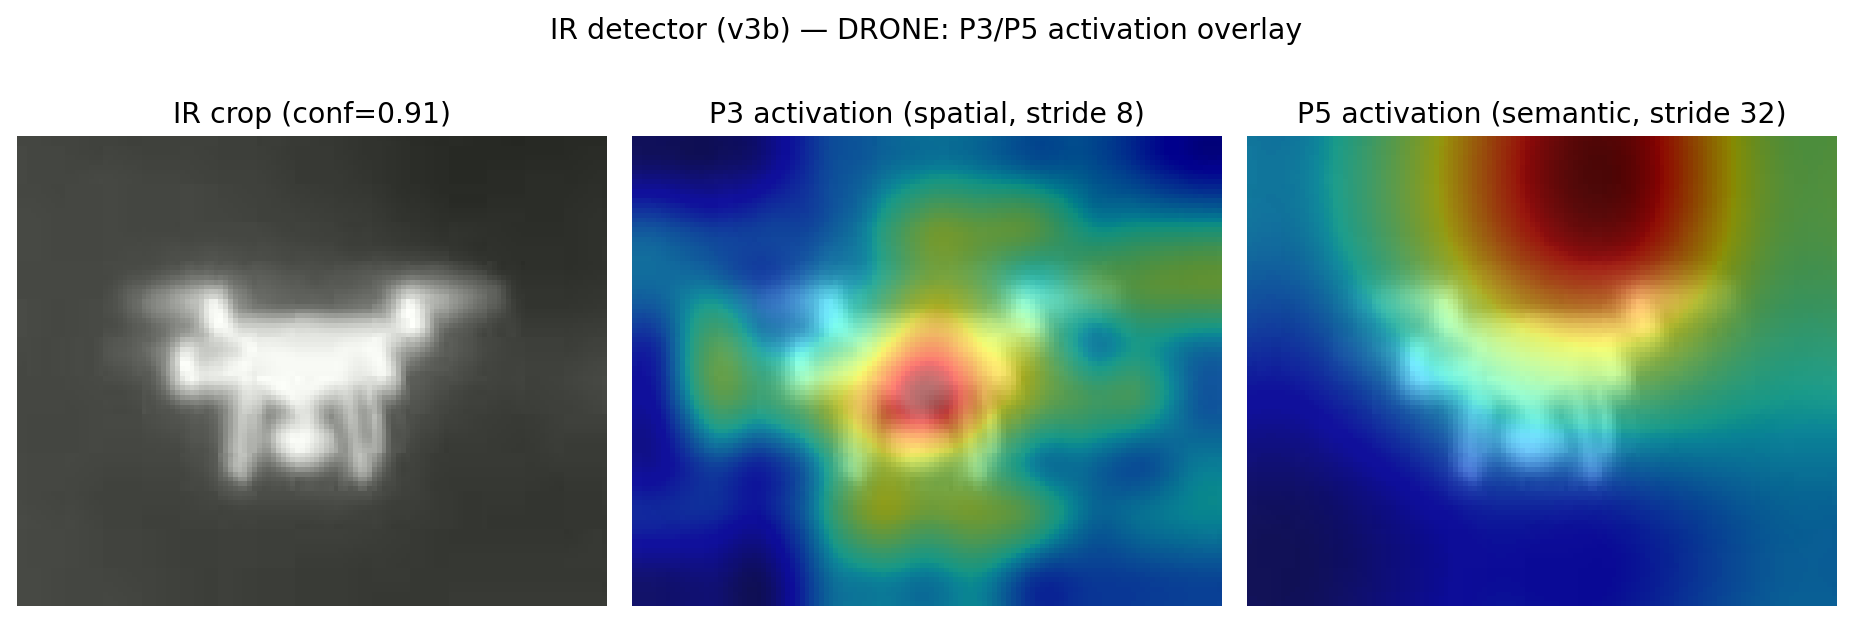
\includegraphics[width=\textwidth]{fig8_mri_ir_act_drone}\caption{Thermal drone (\texttt{IR\_dset\_final})}\end{subfigure}
    \\[4pt]
    \begin{subfigure}{\textwidth}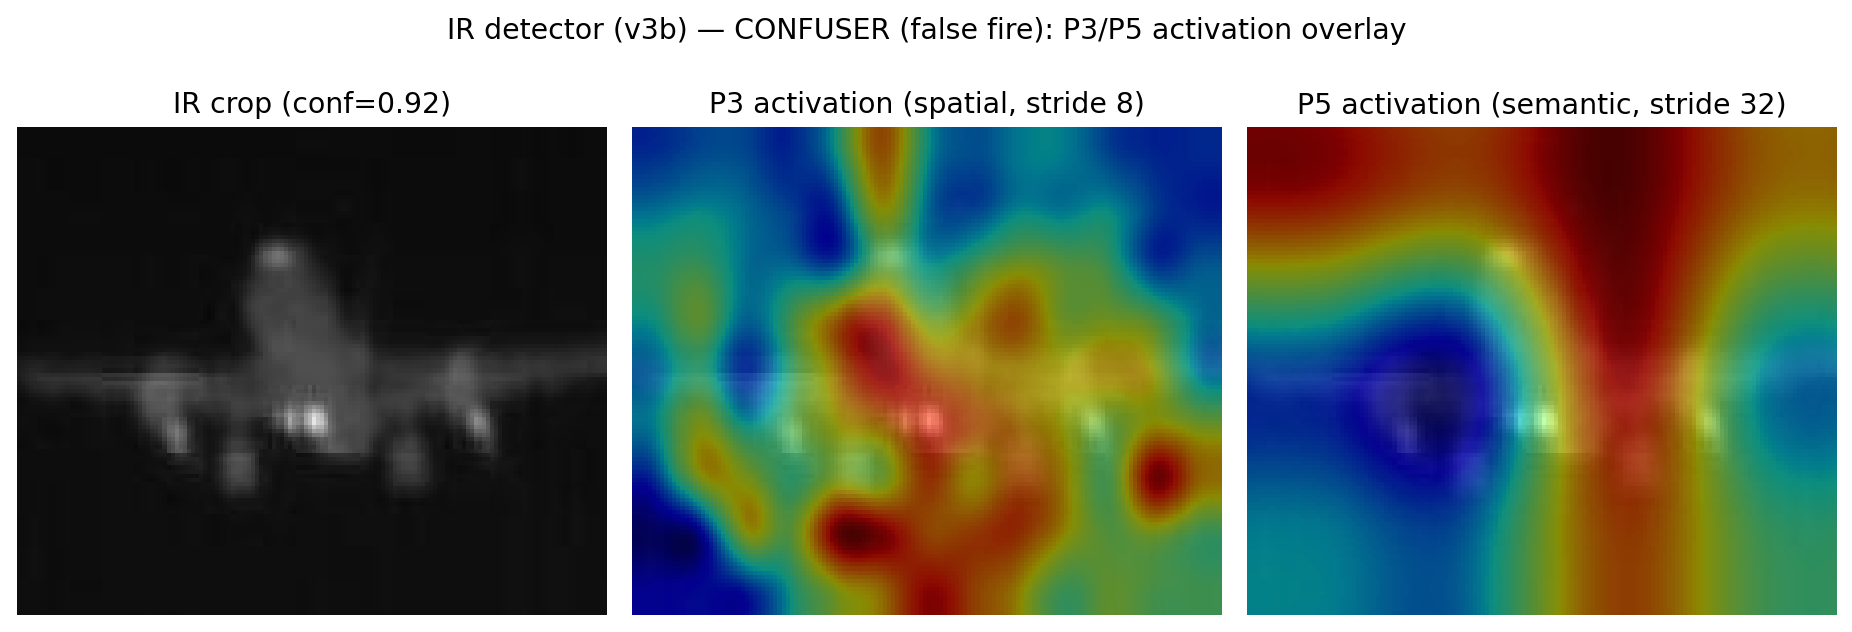
\includegraphics[width=\textwidth]{fig8_mri_ir_act_confuser}\caption{Confuser false-fire (CBAM, held out)}\end{subfigure}
    \caption{Model MRI spatial activation overlay for the IR detector (\texttt{v3b}) --- the thermal counterpart of Figure~\ref{fig:mri_activation}. Each row: the detection crop, the \texttt{p3} activation (stride~8, fine spatial detail), and the \texttt{p5} activation (stride~32, semantic depth). On the thermal drone (a) the activations concentrate on the object; on the confuser false-fire (b) they scatter across background structure. Source: \texttt{scripts/visualize\_ir\_activation.py}; \textsc{Ledger}~ir-features-separable.}
    \label{fig:ir_mri_activation}
\end{figure}

\emph{Second, the grayscale$\rightarrow$thermal feature gap is a removable affine offset, so a confuser filter transfers across the modality.} The detector represents a given class almost identically in real thermal and in grayscale-RGB: the top-discriminative neurons overlap (Jaccard $0.71$--$0.88$), the mean-activation signatures correlate at $0.93$--$0.99$, and the drone-class centroids sit at cosine distance $0.012$. The only systematic difference is a per-feature mean/scale offset. Removing it with a \emph{per-modality z-score} (\S\ref{sec:model_mri}) lifts grayscale$\rightarrow$thermal confuser-transfer AUROC from $0.500$ (chance, no alignment) to $0.919$, against a within-thermal cross-validated ceiling of $0.974$; full-covariance CORAL reaches only $0.707$, which confirms the gap is a diagonal mean/scale shift rather than a representational change (Figure~\ref{fig:ir_gray_align}).
% [source: ledger=gray-thermal-alignable; eval=none (MRI modality probe); run=mri/modality_align.py; cache=mri/results/ir_v3b_report; config=ir_v3b]

\begin{figure}[htbp]
    \centering
    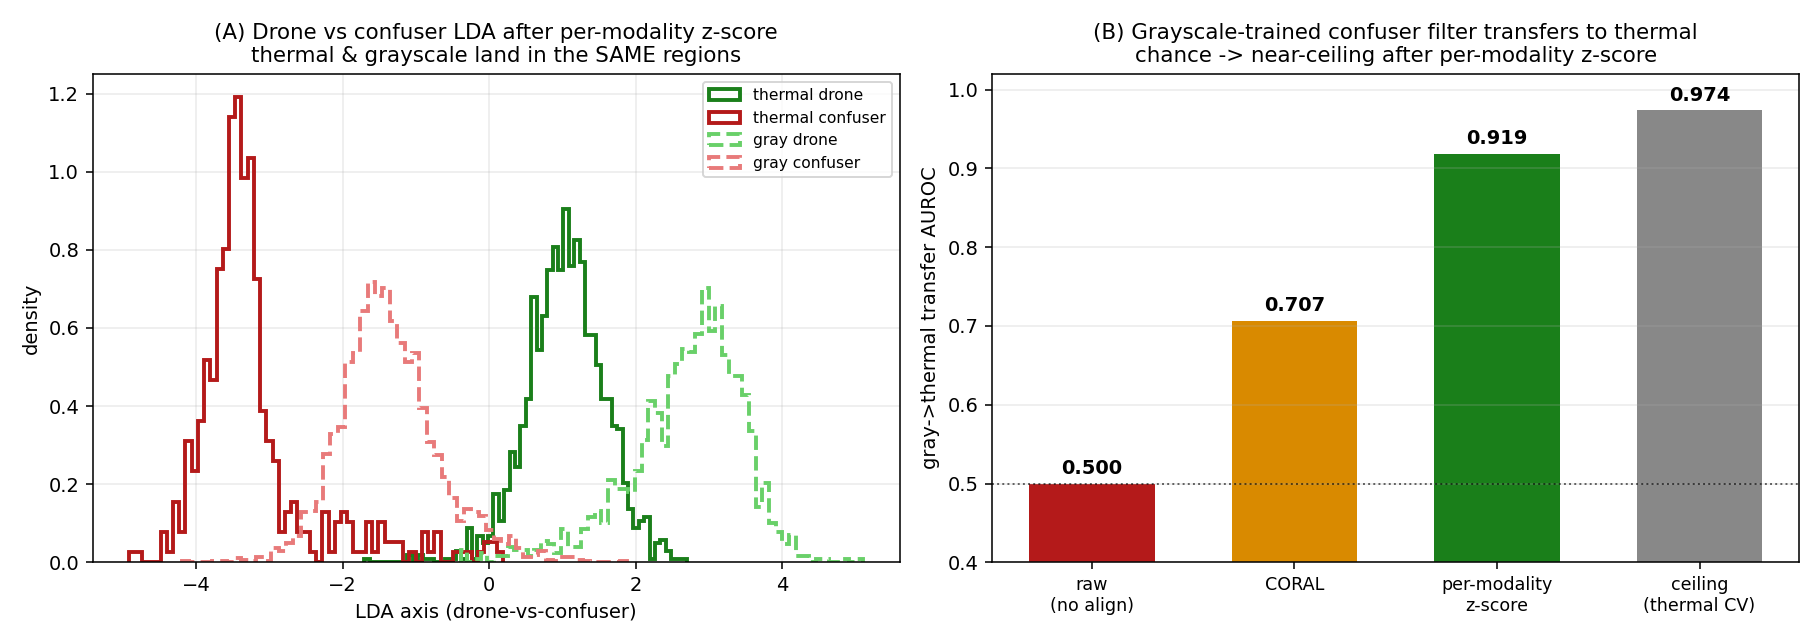
\includegraphics[width=\textwidth]{fig9_ir_gray_align}
    \caption{Grayscale$\leftrightarrow$thermal feature alignment in the IR detector. (A) After a per-modality z-score, thermal and grayscale drones land in the same region of the drone-vs-confuser discriminant axis, and likewise for confusers --- the modalities are interchangeable up to an affine offset. (B) Grayscale-trained confuser-filter transfer to thermal rises from chance ($0.500$) to near the within-thermal ceiling ($0.919$ vs $0.974$) once the offset is removed; CORAL ($0.707$) under-performs the simpler z-score. Source: \textsc{Ledger}~gray-thermal-alignable.}
    % [source: ledger=gray-thermal-alignable; eval=none (MRI modality probe); run=mri/modality_align.py; cache=mri/results/ir_v3b_report; config=ir_v3b]
    \label{fig:ir_gray_align}
\end{figure}

Together these mean the IR confuser-verifier blocker was confuser \emph{data scarcity}, not the detector: labelled thermal confusers are rare, but grayscale-RGB confusers are abundant and, once z-aligned, occupy the same thermal feature space. Harvesting them yields a thermal verifier that is simultaneously confuser-rich and recall-safe; the deployed checkpoint and its held-out evaluation --- which reverses the project's earlier ``ship no IR verifier'' conclusion --- are reported in \S\ref{sec:grayscale_verifier}. The mode was never trained on grayscale, so the cross-modal equivalence is a measured emergent property, not a designed one.
% [source: ledger=ir-grayscale-harvest-solves-thermal-verifier; eval=ir_aligned_cbam_heldout; run=mri_train_aligned; config=cbam_ir_640]

\section{Trust Classifier}
\label{sec:trust_classifier}

\subsection{Feature Set}

The trust classifier consumes per-frame features extracted from the two detectors' raw outputs and the source frames. The exact feature set is variant-dependent. The shipped classifier is the six-feature \texttt{robust6} (\S\ref{sec:feature_selection}); the hand-engineered comparison set is \texttt{scene\_aware\_v3more\_32feat} (\texttt{sa32}, 32 features, failure-model scores dropped) and the two 40-feature variants \texttt{control\_v3more\_40feat} and \texttt{fusion\_no\_fn\_v1.1} (differing in which extra eight features they include). The families of features are common across the larger variants:
% [source: ledger=ft4-lean-trust-classifier; eval=clf_own_holdout; run=classifier/train_lean_ft4.py; config=clf_own_holdout]

\begin{itemize}
    \item \textbf{Detector signals}: per-modality binary detection flags, top-$k$ confidence scores, detection counts.
    \item \textbf{Scene features}: image intensity statistics, edge density, frequency-domain summaries; intended to detect ``confuser-rich'' scenes vs ``clean sky'' scenes.
    \item \textbf{Target features}: bounding-box geometry (aspect ratio, normalised area, position), confidence distribution per modality.
    \item \textbf{Agreement features}: cross-modal IoU, centre distance, confidence ratio.
    \item \textbf{Failure-model scores} (only in \texttt{control\_v3more\_40feat}): scalar outputs from a small per-modality failure-prediction network. \texttt{fusion\_no\_fn\_v1.1} explicitly drops these because they over-fitted to training-set artefacts and degraded OOD behaviour (see \S\ref{sec:classifier_variants}).
\end{itemize}

The label space is the 4-way trust decision of \S\ref{sec:trust_fusion}. The model is an XGBoost~\cite{chen2016xgboost} gradient-boosted classifier. Training uses sequence-stratified group shuffling so that frames from a given Anti-UAV or Svanstr\"om sequence are not split across train and test; this avoids the easy-leakage variant of cross-validation common in video classification.

The Svanstr\"om frames used to train the classifier overlap with the frames used to evaluate the full cascade in Chapter~\ref{ch:experiments}; this is flagged as a threat to validity (\S\ref{sec:threats}) and partially mitigated by the Anti-UAV results, which are not contaminated.

The classifier's value depends jointly on the evaluation surface and the classifier variant. The three-surface behaviour --- a small in-distribution $F1$ cost on Svanstr\"om, substantial OOD-suppression on the synthetic zoo, and a net $F1$ gain on the real-video diagnostic when paired with temporal smoothing --- is quantified in \S\ref{sec:classifier_compare} (this chapter) and Chapter~\ref{ch:experiments} (\S\S\ref{sec:cumulative}, \ref{sec:realvideo_classifier}). The next subsection describes the three classifier variants and their comparative performance.

\subsection{Classifier Variants}
\label{sec:classifier_variants}

Three hand-engineered classifier variants form the comparison set that motivated the production classifier. They are trained against the same labelled paired-frame data and differ in feature engineering and in resilience to OOD distribution shift. The strongest of them on the joint axis is \texttt{scene\_aware\_v3more\_32feat} (hereafter \texttt{sa32}); it was the working pick through the real-video classifier comparison (\S\ref{sec:realvideo_classifier}), with \texttt{fusion\_no\_fn\_v1.1} retained as an open-world fallback and \texttt{control\_v3more\_40feat} deprecated. The shipped classifier is not in this hand-engineered set: it is the six-feature, leakage-aware \texttt{robust6} derived statistically in \S\ref{sec:feature_selection}, which keeps \texttt{sa32}'s in-domain accuracy while dropping the scene-fingerprint features that cost OOD generalisation. The three variants below are therefore best read as the comparison and ablation set against which \texttt{robust6} is measured, not as the shipped stack.
% [source: ledger=ft4-lean-trust-classifier,robust6-production-viable,fusion-feature-leakage; eval=clf_own_holdout; run=classifier/train_lean_ft4.py; cache=docs/analysis/2026-05-31_ft4_lean_trust_classifier.md; config=clf_own_holdout]

\begin{itemize}
    \item \textbf{\texttt{scene\_aware\_v3more\_32feat} (\texttt{sa32}; strongest hand-engineered variant, superseded by \texttt{robust6})}: 32-feature variant with the failure-model scores dropped. Wins on the real-video diagnostic by 18--22 pp drone segment $F1$ over \texttt{control\_v3more\_40feat} and by 60+ pp over \texttt{fusion\_no\_fn\_v1.1} (\S\ref{sec:realvideo_classifier}). Ties \texttt{control\_v3more\_40feat} on Svanstr\"om within 1.3 pp drone $F1$ (\textsc{Ledger}~\S7) and ties it on the OOD confuser zoo (S2 fire 0.205 vs 0.212; S3 fire 0.103 vs 0.094; \textsc{Ledger}~\S7). Higher OOD-zoo fire rate than \texttt{fusion\_no\_fn\_v1.1}, which is the operational cost of its drone-recall preservation.
    % [source: ledger=three-classifier-realvideo; eval=pipe3clf_sa32; run=(EVIDENCE_LEDGER sweep); config=pipe_video_drone_iop]
    \item \textbf{\texttt{fusion\_no\_fn\_v1.1} (open-world fallback)}: 40-feature variant trained with the failure-model scores explicitly dropped, sourced from the legacy fusion training pipeline. Substantially more conservative on OOD imagery ($\sim$1.6\% S2 zoo fire rate vs 20.5\% for sa32, a 13$\times$ reduction), but rejects 85\% of correct RGB drone TPs on the real-video diagnostic (\S\ref{sec:realvideo_classifier}, segment-level drone $R$ collapses to $0.128$ for baseline RGB). The right choice when missed drones cost less than confuser-induced false alarms; the wrong choice for general-purpose alert deployment.
    % [source: ledger=cascade-confuser-collapse; eval=pipe3clf_fnfn; run=(EVIDENCE_LEDGER sweep); config=pipe_video_drone_iop]
    \item \textbf{\texttt{control\_v3more\_40feat} (deprecated)}: 40-feature variant with failure-model scores retained. Equivalent to sa32 on Svanstr\"om and on the OOD confuser zoo within rounding, but loses 18--22 pp drone segment $F1$ on the real-video diagnostic. No operational regime favours it over sa32 on the joint axis; it was a production candidate prior to the real-video classifier comparison and is retained in the comparison tables for completeness.
\end{itemize}

The early \texttt{retrained\_v2\_32feat} classifier (trained against the \texttt{retrained\_v2} RGB detector) is also superseded because the production RGB detector is no longer \texttt{retrained\_v2}. The mismatch between the classifier's training-time RGB confidence distribution and the production RGB confidence distribution accounts for the bulk of the gap in classifier-comparison results (\textsc{Ledger}~\S5). A single trust classifier is not portable across arbitrary RGB detector swaps without re-checking calibration.

\paragraph{Scene-fingerprint over-fitting.}
A feature-selection finding shaped the lean feature set that the production classifier later formalised. Under sequence-stratified splitting, per-clip image statistics --- absolute brightness scalars and the normalised horizontal position $\mathit{pos\_x}$ --- act as \emph{scene fingerprints}: the classifier learns to recognise which clip a frame came from rather than whether a drone is present, which inflates in-distribution scores but degrades transfer to held-out clips. Dropping these features (the \texttt{lean13}$\to$\texttt{lean10} feature set) recovers $18$--$26$~pp drone $F1$ on held-out drone clips. The \texttt{scene\_aware\_v3more\_32feat} (\texttt{sa32}) variant therefore already omits the scene-fingerprint features by design. \S\ref{sec:feature_selection} turns this hindsight observation into a statistic computed \emph{before} training and uses it to derive a six-feature classifier from first principles.
% [source: ledger=scene-fingerprint-overfit; eval=own_lean10_yt,own_lean13_yt; run=(classifier feature-selection ablation); config=clf_own_holdout]

\paragraph{A dual-classifier extension for the missing-modality regime.}
A single classifier must serve both the paired RGB+IR regime and the grayscale-only fallback, whose feature distributions differ. Splitting it into a \emph{dual} architecture --- a 24-feature paired model and a separate 32-feature grayscale model --- strictly dominates single \texttt{sa32} on the missing-modality cases: on the RGB-fallback bird-confuser the drone $F1$ rises $0.247\to1.000$, on the \texttt{drone\_seagull} clip $0.461\to0.942$, and on \texttt{rgb\_dataset\_test} $0.690\to0.960$, while the paired-core performance is unchanged. The grayscale-fallback airplane and helicopter cases remain weak ($F1\approx0.50$, pending further hard-negative mining), so the dual classifier is reported as a validated extension rather than the shipped default.
% [source: ledger=dual-classifier-v3; eval=dualclf_v3_vs_sa32; run=(EVIDENCE_LEDGER sweep); config=dual_clf_v3_surfaces]

\paragraph{A grayscale-fallback recall hole in \texttt{robust6}.}
The \texttt{robust6} classifier (\S\ref{sec:feature_selection}; the base for the shipped \texttt{robust8}) inherits one honest weakness from its lean feature set. In the grayscale-RGB fallback regime (no thermal sensor), all three of \texttt{robust6}'s IR features and the cross-modal ratio go to chance (single-feature AUROC $\approx 0.51$) because the IR inputs are dead, leaving only the RGB features and \texttt{conf\_sum} live. The consequence is a \texttt{trust\_rgb} \emph{recall} failure: drone-only-in-RGB frames are routed to \texttt{reject}, and grayscale drone recall collapses to $R\approx0.19$, while \texttt{trust\_both} ($F1\approx0.98$) and thermal \texttt{trust\_ir} ($\approx0.92$) remain healthy. The first reading was that this needs an architectural fix (regime-aware routing); \S\ref{sec:feature_selection} shows instead that two free features (\texttt{rgb\_mean\_conf} and an \texttt{is\_grayscale} flag) and a per-class \texttt{trust\_rgb} threshold close it --- the \texttt{robust8} extension --- recovering grayscale recall at a measured real-video-confuser cost.
% [source: ledger=robust6-grayscale-ir-features-dead,routing-failure-is-trust-rgb-recall; eval=clf_own_holdout; run=classifier/train_lean_ft4.py; config=clf_own_holdout]

\subsection{Classifier Performance Comparison}
\label{sec:classifier_compare}

Three classifier variants were compared in the same harness on Svanstr\"om (stride 9; IoP@0.5; baseline RGB; v2 patch verifier; \texttt{imgsz=1280}; \textsc{Ledger}~\S7) and on the OOD confuser zoo:

\begin{table}[htbp]
    \centering
    \caption{Classifier comparison. The split verdict between Svanstr\"om and the OOD zoo motivates the open-world vs calibrated-deployment distinction. Source: \textsc{Ledger}~\S7.}
    \label{tab:classifiers}
    \begin{tabular}{lccccccc}
        \toprule
        Classifier & thr & Drone S2 $R$ & Drone S2 F1 & Drone S3 $R$ & Drone S3 F1 & Zoo S2 & Zoo S3 \\
        \midrule
        \texttt{fusion\_no\_fn\_v1.1}        & 0.8/0.9 & 0.909 & 0.912 & 0.856/0.869 & 0.889/0.895 & \textbf{0.016} & \textbf{0.008} \\
        \textbf{\texttt{scene\_aware\_v3more\_32feat}} & 0.8 & 0.922 & 0.919 & 0.868 & 0.896 & 0.205 & 0.103 \\
        \texttt{control\_v3more\_40feat} & 0.9 & \textbf{0.934} & \textbf{0.925} & \textbf{0.893} & \textbf{0.909} & 0.212 & 0.094 \\
        \bottomrule
    \end{tabular}
\end{table}

\begin{figure}[htbp]
    \centering
    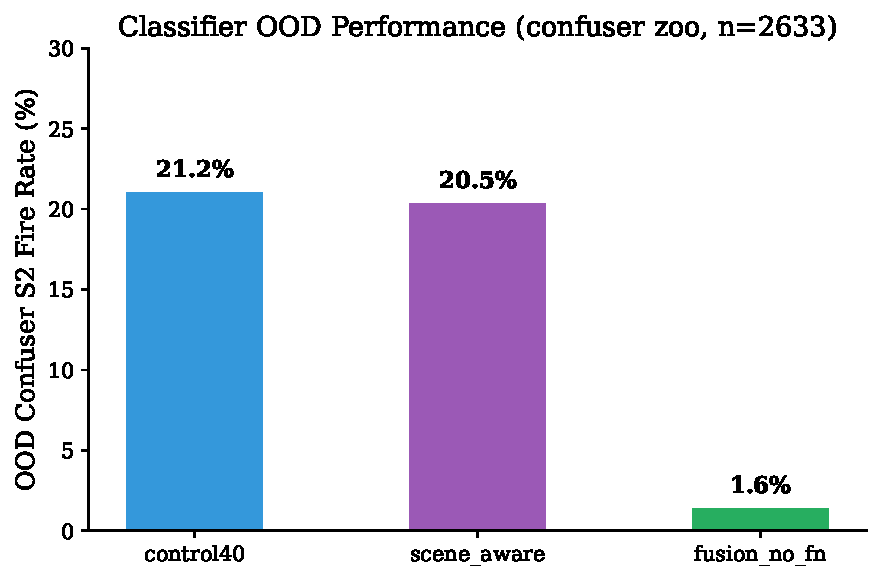
\includegraphics[width=0.85\textwidth]{fig7_1_ood_classifier}
    \caption{Classifier comparison on the OOD confuser zoo. \texttt{fusion\_no\_fn\_v1.1} fires on $\sim$13$\times$ fewer frames than the comparison classifier \texttt{sa32} and the deprecated \texttt{control\_v3more\_40feat}; sa32 and control40 are tied within rounding on this benchmark. Source: \textsc{Ledger}~\S7 + \texttt{eval/results/\_cumulative\_halluc/confuser\_c40/summary.json}.}
    \label{fig:ood_classifier}
\end{figure}

Three readings, ordered by the surface that drives the production decision.

\emph{Svanstr\"om.} \texttt{control\_v3more\_40feat} wins on every Svanstr\"om drone metric ($+2.5$~pp Stage-3 recall vs \texttt{scene\_aware}; $+1.3$~pp Stage-3 F1). \texttt{fusion\_no\_fn\_v1.1} is roughly tied. Within 1.3 pp drone F1 the three are operationally indistinguishable on this benchmark.

\emph{OOD confuser zoo.} \texttt{fusion\_no\_fn\_v1.1} is \emph{13$\times$ more conservative} than \texttt{scene\_aware} (1.6\% vs 20.5\% S2 fire). \texttt{control\_v3more\_40feat} ties \texttt{scene\_aware} (0.212 vs 0.205 S2; 0.094 vs 0.103 S3). The fnfn-vs-sa32 gap is therefore real and load-bearing; the control40-vs-sa32 gap on the zoo is not.
% [source: ledger=cascade-confuser-collapse; eval=clfzoo_fnfn; run=eval/cumulative_halluc.py; cache=eval/results/_cumulative_halluc/confuser_fusion_no_fn_model_v1.1/summary.json; config=confuser_zoo_1280]

\emph{Real video} (\S\ref{sec:realvideo_cascade}; \textsc{Ledger}~\S9.5.8). \texttt{scene\_aware} dominates: cascade drone segment $F1$ = 0.826 baseline RGB, vs 0.644 for \texttt{control\_v3more\_40feat} ($-18$~pp) and 0.219 for \texttt{fusion\_no\_fn\_v1.1} ($-61$~pp). The Svanstr\"om-only ordering reverses on real-video; the Svanstr\"om benchmark does not by itself select the production classifier.
% [source: ledger=three-classifier-realvideo; eval=pipe3clf_sa32; run=(EVIDENCE_LEDGER sweep); config=pipe_video_drone_iop]

\paragraph{Deployment implication.}
Among the hand-engineered variants \texttt{scene\_aware\_v3more\_32feat} (\texttt{sa32}) is the strongest: it ties or wins on every surface except a single 1.3-pp gap on Svanstr\"om S3 F1 (where \texttt{control\_v3more\_40feat} edges it by a margin smaller than typical run variance), and it strictly dominates on the real-video diagnostic. \texttt{control\_v3more\_40feat} buys nothing on the zoo over sa32 and loses on real-video; it is retained in this table for completeness and reproducibility but is deprecated. \texttt{fusion\_no\_fn\_v1.1} remains the open-world fallback for surfaces where confuser noise dominates and missed drones are operationally tolerable. \texttt{sa32} is therefore the reference the production classifier must match: \S\ref{sec:feature_selection} shows the six-feature \texttt{robust6} holds \texttt{sa32}'s in-domain accuracy while improving OOD-confuser robustness, and its grayscale-hardened extension \texttt{robust8}---not \texttt{sa32}---is the shipped classifier.
% [source: ledger=robust6-production-viable; eval=clf_own_holdout; run=eval/overnight_ablation.py; cache=eval/results/_overnight_ablation/ablation_results.json; config=clf_own_holdout]

\subsection{Statistical Feature Selection: a Six-Feature Classifier}
\label{sec:feature_selection}

The variants above were assembled by hand: a feature family was included or dropped on the basis of intuition and post-hoc held-out checks (the \texttt{lean13}$\to$\texttt{lean10} pruning of \S\ref{sec:classifier_variants} is the clearest case). This subsection replaces that procedure with a statistical one. The motivating question is whether the $32$-feature production classifier needs all $32$ features, or whether a measurable property can identify in advance which features carry the drone-versus-confuser signal and which only memorise scenes. Two practical pressures sharpen the question. The incumbent \texttt{sa32} was trained on detections from the superseded \texttt{selcom\_1280} detector, so its inputs no longer match the production \texttt{ft4} RGB / \texttt{v3b} IR detectors. Several of its features are also per-frame image statistics that require a full image read and OpenCV pass per frame, the most expensive features in the set.
% [source: ledger=fusion-feature-leakage; eval=clf_own_holdout; run=classifier/fusion_feature_stats.py; cache=classifier/fusion_models/optimal_v1/feature_stats_ranked.csv; config=clf_own_holdout]

\paragraph{Method.}
From a cached $56$-feature matrix of $65{,}192$ frames (\texttt{classifier/fusion\_models/optimal\_v1/fusion\_dataset\_full56.csv}) we ran four analyses, each answering one question. Linear discriminant analysis asks whether the signal is present at all: a single Fisher axis separates the trust-positive from the reject class at $98.2\%$ training accuracy (Figure~\ref{fig:fusion_lda}), so the signal is strong and largely linear, and the problem is one of \emph{selecting} features rather than a shortage of signal. An unsupervised PCA projection asks whether the structure is trivial: the classes overlap in the top principal components (Figure~\ref{fig:fusion_pca}), which means the dominant axis of variance is scene-to-scene difference (brightness, texture) rather than the drone signal --- the first indication that scene-statistic features dominate variance without carrying class signal. A per-feature ANOVA $F$-test and single-feature AUROC then rank each feature by how well it alone separates the two classes (Figure~\ref{fig:fusion_auroc}).
% [source: ledger=fusion-feature-leakage; eval=clf_own_holdout; run=classifier/fusion_feature_stats.py; cache=classifier/fusion_models/optimal_v1/feature_stats_ranked.csv; config=clf_own_holdout]

\paragraph{A leakage statistic.}
A scene-fingerprint feature such as \texttt{img\_mean} can score as discriminative in a single pool simply because it correlates with which scene a sample came from, and scenes correlate with labels in the training data; ANOVA and AUROC, computed on one pool, would recommend keeping it. To expose this we compute a second $F$-statistic \emph{within the drone class only} --- how much the feature varies by scene among samples that all share the same label --- and form the ratio
\begin{equation}
\mathit{leakage\_ratio} = \frac{F_\text{domain-in-class}}{F_\text{class}},
\label{eq:leakage}
\end{equation}
which is low for a robust signal feature (its value barely changes by scene within drones) and high for a scene fingerprint (its value is almost entirely scene-determined). Equation~\ref{eq:leakage} converts the earlier hand-tuned deprecations into a number computed before any training run. It is conceptually adjacent to domain-adaptation distribution-alignment ideas, but inverts their use: rather than aligning features across domains, the statistic \emph{measures} a feature's domain-dependence in order to discard it.
% [source: ledger=fusion-feature-leakage; eval=clf_own_holdout; run=classifier/fusion_feature_stats.py; cache=classifier/fusion_models/optimal_v1/feature_stats_ranked.csv; config=clf_own_holdout]

\begin{figure}[htbp]
    \centering
    \begin{subfigure}{0.48\textwidth}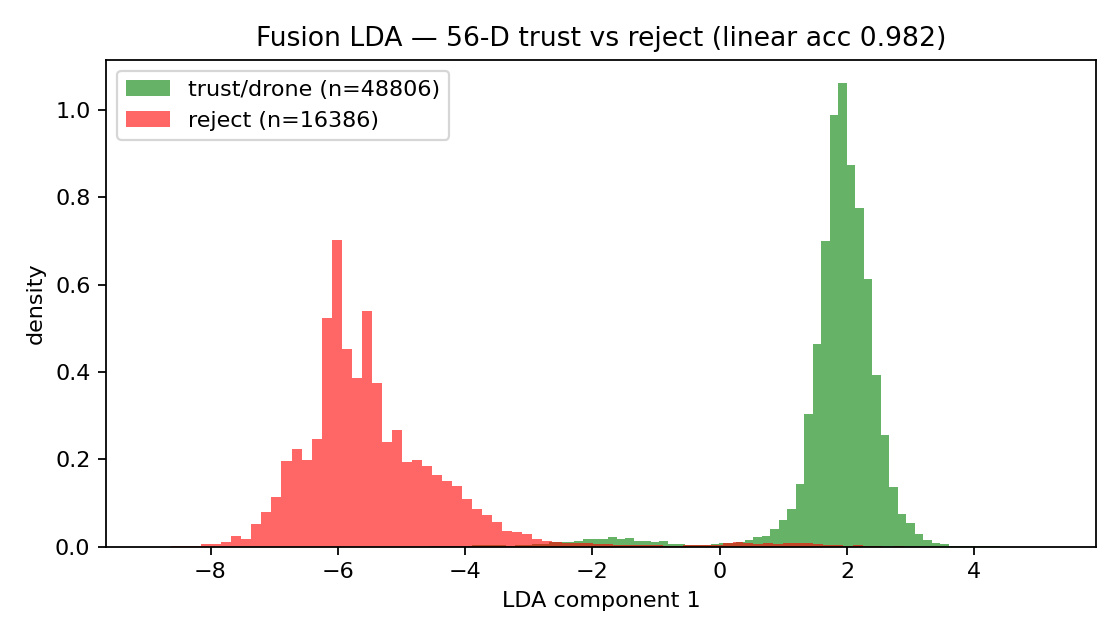
\includegraphics[width=\textwidth]{fig8_fusion_lda}\caption{}\label{fig:fusion_lda}\end{subfigure}
    \hfill
    \begin{subfigure}{0.48\textwidth}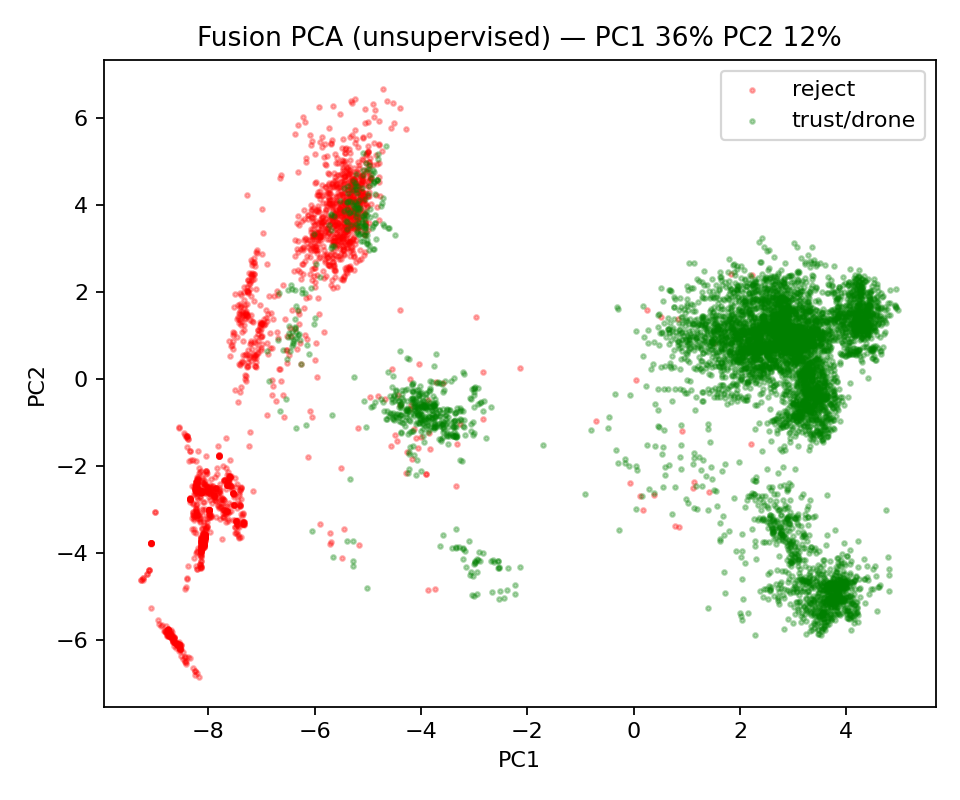
\includegraphics[width=\textwidth]{fig8_fusion_pca}\caption{}\label{fig:fusion_pca}\end{subfigure}
    \\[4pt]
    \begin{subfigure}{0.48\textwidth}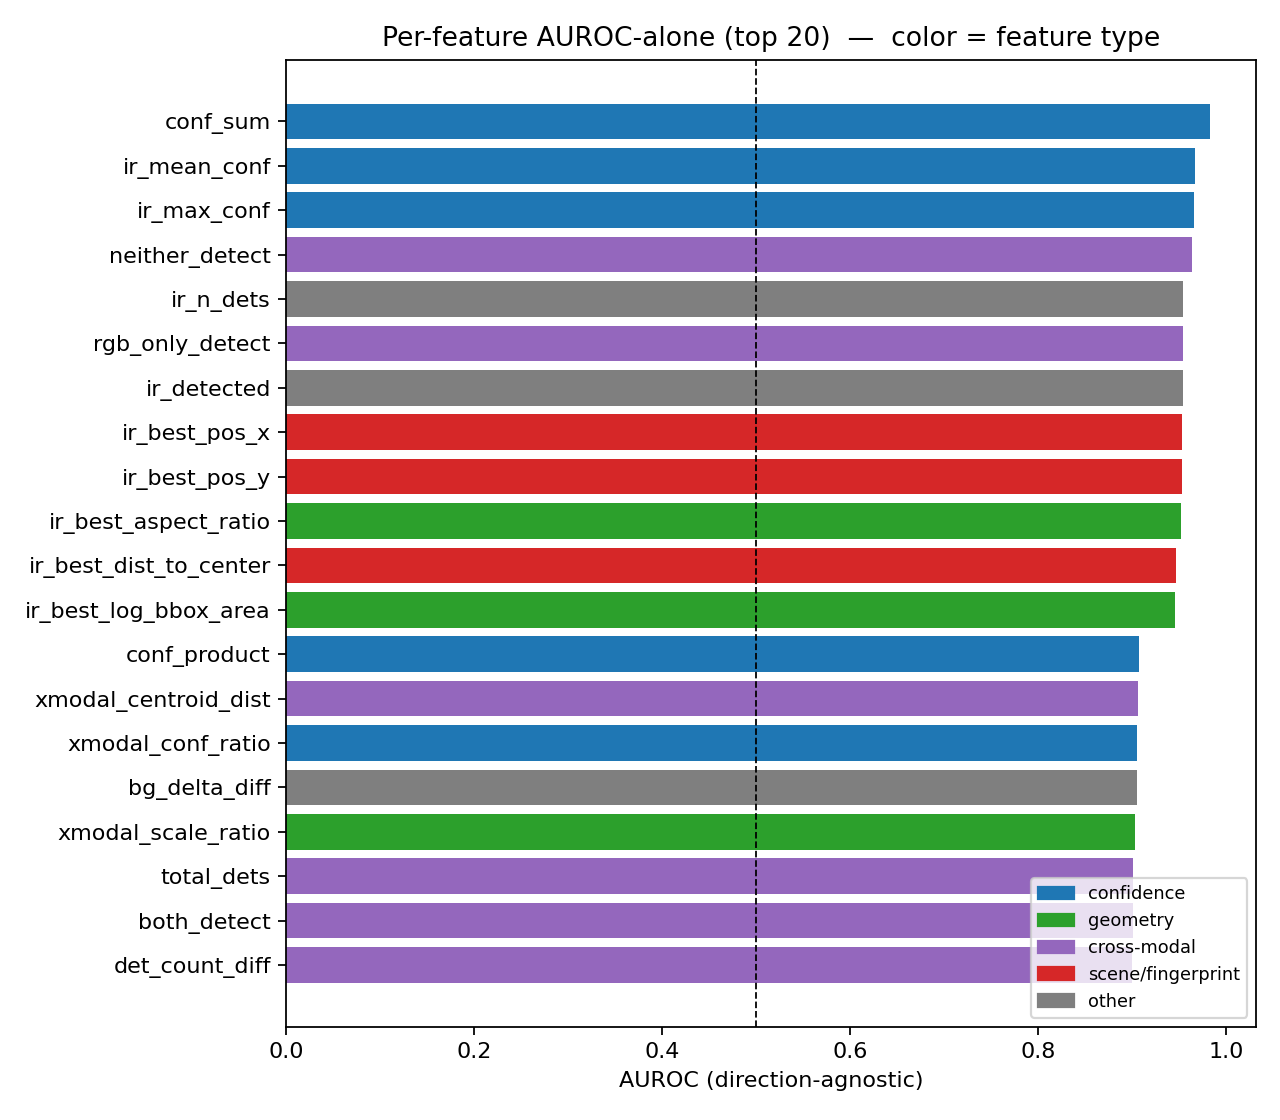
\includegraphics[width=\textwidth]{fig8_fusion_auroc}\caption{}\label{fig:fusion_auroc}\end{subfigure}
    \hfill
    \begin{subfigure}{0.48\textwidth}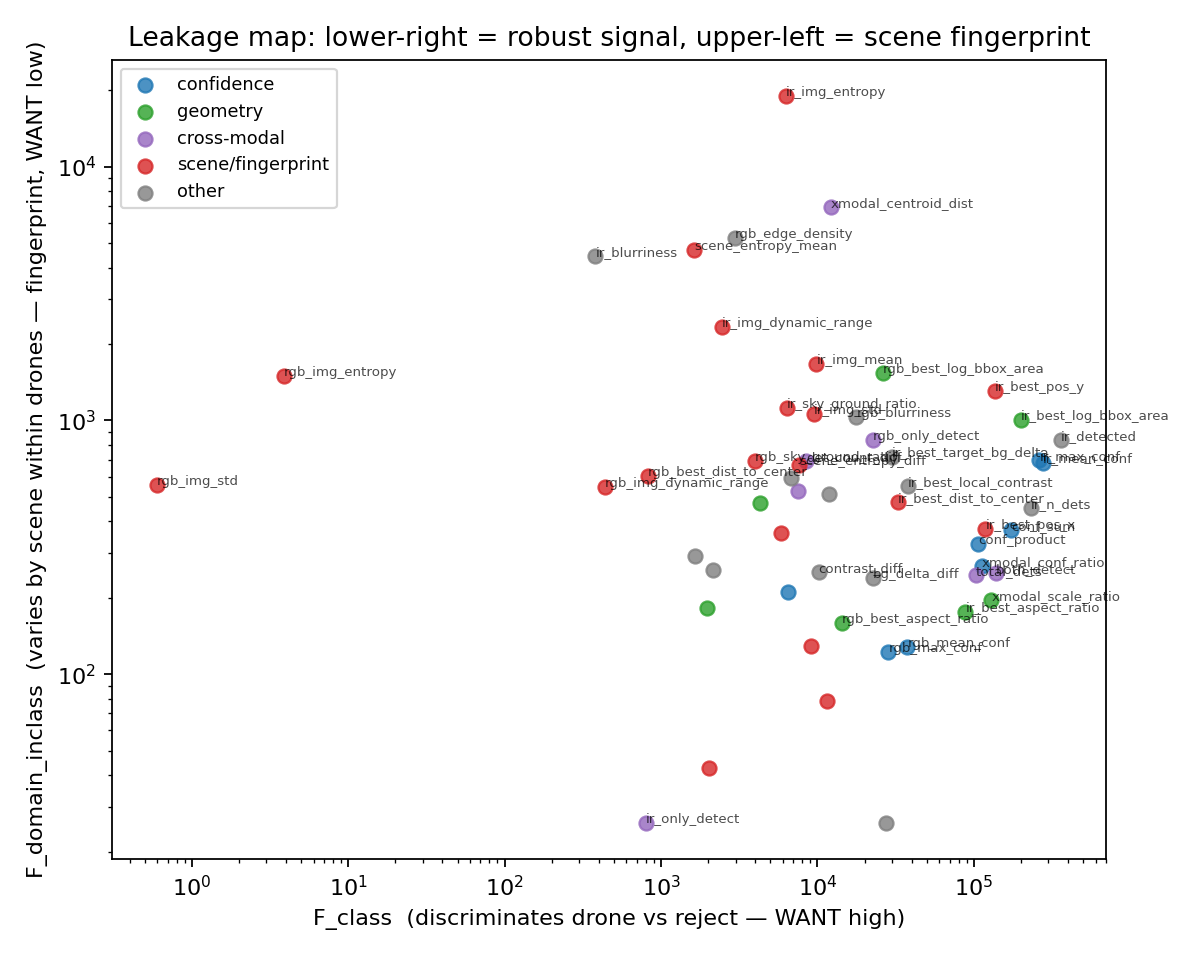
\includegraphics[width=\textwidth]{fig8_fusion_leakage}\caption{}\label{fig:fusion_leakage}\end{subfigure}
    \caption{Statistical anatomy of the $56$-feature fusion space. (a) Linear discriminant: the trust signal is linearly separable ($98.2\%$ train accuracy). (b) Unsupervised PCA: the classes overlap, so the dominant variance is scene difference, not the class signal. (c) Per-feature single-feature AUROC. (d) Leakage map (Eq.~\ref{eq:leakage}): the lower-right region is robust signal (high AUROC, near-zero leakage); the upper-left is scene fingerprint (chance-level AUROC, leakage in the hundreds). Source: \textsc{Ledger}~fusion-feature-leakage; \texttt{classifier/fusion\_feature\_stats.py}.}
    % [source: ledger=fusion-feature-leakage; eval=clf_own_holdout; run=classifier/fusion_feature_stats.py; cache=classifier/fusion_models/optimal_v1/feature_stats_ranked.csv; config=clf_own_holdout]
    \label{fig:fusion_stats}
\end{figure}

\paragraph{What the statistic finds.}
The leakage map separates two groups cleanly (Table~\ref{tab:leakage}). The scene-statistic features score at chance on the class label (\texttt{rgb\_img\_std} AUROC $0.502$, \texttt{rgb\_img\_entropy} $0.510$) yet have leakage ratios in the hundreds ($349.6$ and $307.4$) --- they discriminate \emph{which scene}, not whether a drone is present. These are precisely the expensive per-frame features, so the statistic flags them as both dangerous and costly. The robust core --- detection confidences, box geometry, and cross-modal ratios --- scores AUROC above $0.9$ with leakage below $0.006$. A complementary within-source check guards against a case the leakage ratio alone misses: \texttt{rgb\_blurriness} scores a respectable pooled AUROC ($0.872$) yet collapses to chance \emph{within} each source ($0.516$), exposing it as a cross-clip mean-shift artifact rather than a drone signal, so the gate drops it alongside the scene fingerprints. Two caveats are recorded honestly. The per-modality detection-presence flags top the AUROC chart but are excluded by reasoning rather than by Equation~\ref{eq:leakage}: the trust label is \emph{derived from} those detections, so they leak the label, and the leakage statistic catches scene leakage, not label leakage. And the corpus is IR-dominant (Anti-UAV-heavy), so IR features rank above their RGB counterparts; on RGB-fallback surfaces the balance shifts.
% [source: ledger=fusion-feature-leakage,blurriness-is-corpus-artifact; eval=clf_own_holdout; run=classifier/fusion_feature_stats.py,classifier/vet_blurriness_stats.py; cache=classifier/fusion_models/optimal_v1/feature_stats_ranked.csv; config=clf_own_holdout]

\begin{table}[htbp]
    \centering
    \caption{Leakage analysis splits the feature space. \emph{Top}: scene fingerprints --- chance-level class AUROC but very high leakage; drop. \emph{Bottom}: the robust core --- high AUROC, near-zero leakage; keep. Source: \textsc{Ledger}~fusion-feature-leakage; \texttt{feature\_stats\_ranked.csv}.}
    \label{tab:leakage}
    \begin{tabular}{llcc}
        \toprule
        feature & family & AUROC-alone & leakage ratio \\
        \midrule
        \multicolumn{4}{l}{\emph{Scene fingerprints (drop)}} \\
        \texttt{rgb\_img\_std}       & scene       & 0.502 & 349.6 \\
        \texttt{rgb\_img\_entropy}   & scene       & 0.510 & 307.4 \\
        \texttt{ir\_blurriness}      & scene       & 0.795 & 11.7 \\
        \texttt{rgb\_edge\_density}  & scene       & 0.525 & 1.75 \\
        \midrule
        \multicolumn{4}{l}{\emph{Robust core (keep)}} \\
        \texttt{conf\_sum}             & confidence  & 0.983 & 0.002 \\
        \texttt{ir\_max\_conf}         & confidence  & 0.965 & 0.002 \\
        \texttt{ir\_best\_aspect\_ratio} & geometry  & 0.952 & 0.002 \\
        \texttt{ir\_best\_log\_bbox\_area} & geometry & 0.946 & 0.005 \\
        \texttt{xmodal\_conf\_ratio}   & cross-modal & 0.905 & 0.002 \\
        \bottomrule
    \end{tabular}
\end{table}

\paragraph{The robust6 classifier.}
Applying the keep rule yields a six-feature set, \texttt{robust6} $=$ \{\texttt{rgb\_max\_conf}, \texttt{ir\_max\_conf}, \texttt{rgb\_best\_log\_bbox\_area}, \texttt{ir\_best\_log\_bbox\_area}, \texttt{rgb\_best\_aspect\_ratio}, \texttt{ir\_best\_aspect\_ratio}\}: all six are free (detector outputs and box geometry, no image reads), all near-zero leakage. We re-mined training data from the \emph{current} detectors (\texttt{ft4} RGB, \texttt{v3b} IR), which fixes the drift in \texttt{sa32}'s inputs, and trained an XGBoost classifier under the same sequence-grouped split so a model cannot pass by memorising a scene. Two ablation levels confirm the design. On the re-mined data, in-domain $F1$ is essentially flat as the feature count grows from $6$ to $32$, so the count is not the lever. But on out-of-distribution drone video, the set \emph{with} fingerprint features collapses to $F1=0.262$, and removing them climbs it to $0.436$ and then to $0.578$ for \texttt{robust6} --- dropping the fingerprints roughly doubles OOD generalisation. The four-feature variant that also drops the IR geometry loses confuser rejection, so the box-geometry features are load-bearing rather than redundant.
% [source: ledger=ft4-lean-trust-classifier; eval=clf_own_holdout; run=classifier/train_lean_ft4.py; cache=docs/analysis/2026-05-31_ft4_lean_trust_classifier.md; config=clf_own_holdout]

\paragraph{Full-pipeline verdict.}
A frame-level alert ablation over $5{,}000$ strided frames per surface, in the production cascade composition, decides production-viability (Table~\ref{tab:robust6_pipeline}). On the in-domain Svanstr\"om surface \texttt{sa32} edges \texttt{robust6} by $0.2$~pp $F1$ ($0.9974$ vs $0.9957$) --- negligible. On the OOD confuser surface \texttt{robust6} is materially better: classifier-only false-alert (fire) rate $0.143$ vs $0.203$, about $30\%$ fewer false alerts on \emph{unseen} confusers, and the best-composed cascade reaches $0.057$ vs $0.066$. On the saturated Anti-UAV surface \texttt{robust6} costs about $0.6$~pp recall. The run also makes a structural point: on surveillance the classifier does the bulk of the false-positive suppression (classifier-only Svanstr\"om fire $0.003$ versus $0.065$ for the verifier alone, roughly $20\times$ better), while on the confuser surface the classifier and verifier are complementary and the lowest fire rate needs both. \texttt{robust6} is therefore production-viable: it trades a hair of in-domain $F1$ for materially better OOD-confuser robustness using six free, drift-proof features in place of \texttt{sa32}'s $32$ (several of them expensive per-frame scene reads). \texttt{sa32} wins only if one optimises purely for the in-domain surface --- the overfitting trap the leakage analysis is designed to avoid. One caveat is logged: in this run the drone surfaces use true thermal IR while the confuser set uses grayscale-fallback IR, a modality split in the classifier's IR features across positives and negatives; it mirrors the deployment fallback policy but is stated explicitly.
% [source: ledger=robust6-production-viable; eval=clf_own_holdout; run=eval/overnight_ablation.py; cache=eval/results/_overnight_ablation/ablation_results.json; config=clf_own_holdout]

\begin{table}[htbp]
    \centering
    \caption{Full-pipeline frame-level alert ablation ($5{,}000$ strided frames/surface, production cascade). \texttt{sa32} edges \texttt{robust6} in-domain (Svanstr\"om $F1$, IoP@0.5); \texttt{robust6} wins out-of-domain (confuser fire rate, lower is better). Fire $=$ false-alert rate on the OOD confuser set. Source: \textsc{Ledger}~robust6-production-viable; \texttt{eval/overnight\_ablation.py}.}
    \label{tab:robust6_pipeline}
    \begin{tabular}{lcc}
        \toprule
        cell & Svanstr\"om $F1$ $\uparrow$ & confuser fire $\downarrow$ \\
        \midrule
        bare (no classifier/verifier)        & 0.715 & 0.379 \\
        verifier only                        & 0.964 & 0.114 \\
        classifier only \texttt{[sa32]}      & 0.9972 & 0.203 \\
        classifier only \texttt{[robust6]}   & 0.9877 & \textbf{0.143} \\
        classifier$\to$verifier \texttt{[sa32]}    & \textbf{0.9974} & 0.079 \\
        classifier$\to$verifier \texttt{[robust6]} & 0.9957 & 0.066 \\
        verifier$\to$classifier \texttt{[robust6]} & --- & \textbf{0.057} \\
        \bottomrule
    \end{tabular}
\end{table}

\paragraph{Closing the grayscale hole: \texttt{robust8}.}
The grayscale \texttt{trust\_rgb} recall hole identified above (\S\ref{sec:classifier_compare}) turns out to be a missing feature plus a decision-rule artifact, not a feature-space limit --- and both fixes are free. On the slice where the hole lives (grayscale frames in which RGB fired but the IR channel is blind), the detector's own mean confidence \texttt{rgb\_mean\_conf} separates drone from confuser at single-feature AUROC $0.934$ --- a learned object signal the six-feature set omitted. Adding it, with an \texttt{is\_grayscale} regime flag, gives the eight-feature \texttt{robust8}. The second half of the fix is the decision rule: argmax over the four-class softmax imposes a far-too-high implicit threshold on the rare \texttt{trust\_rgb} class, so a per-class threshold $\tau$ on $P(\texttt{trust\_rgb})$ converts the now-present signal into recall. Validated end-to-end on the production cascade (\texttt{ft4}/\texttt{v3b}, classifier$\to$verifier, $4{,}000$ frames per surface), \texttt{robust8} at $\tau{=}0.20$ lifts Svanstr\"om-grayscale drone recall $0.577 \to 0.681$ (and to $0.738$ at $\tau{=}0.10$) at unchanged precision ($\approx 0.91$), ties thermal $F1$ ($\approx 0.98$), and lowers the RGB-confuser fire rate. The cost is structural rather than a threshold artifact: real-video-confuser fire rises roughly $7$--$10\times$ ($0.006 \to 0.046$ at $\tau{=}0.20$), because \texttt{rgb\_mean\_conf} reads as a drone on Svanstr\"om but as a confident bird or aircraft on real-motion video, and raising $\tau$ does not remove it. \texttt{robust8} at $\tau{=}0.20$ is therefore the shipped balanced operating point, with \texttt{robust6} the better choice on real-video-confuser-dominated surfaces. The correction came from measuring per-slice AUROC and sweeping the decision threshold rather than trusting aggregate argmax macro-$F1$ --- the same statistics-first discipline behind the leakage rule.
% [source: ledger=robust8-grayscale-router; eval=svan_gray_robust8_t20_clffilter,svan_gray_robust6_clffilter,video_confuser_robust8_t20_clffilter; run=eval/compare_routing_pipeline.py; cache=eval/results/_routing_pipeline_cmp/comparison.md]

\paragraph{Further free levers.}
Two related findings from the same statistics-gated search bound what else is available cheaply. A greedy forward selection over the free feature pool surfaces cross-modal \emph{difference} features (\texttt{pos\_euclidean\_diff}, \texttt{area\_diff}) that beat the expensive scene statistics on grayscale routing (grayscale macro-$F1$ $0.36 \to 0.61$), confirming the gains come from free detector geometry rather than scene reads. A stronger lever still is the verifier's own output: the RGB \texttt{mlp\_v5} drone probability separates trust-positive from reject at AUROC $0.949$ against $0.842$ for raw detection confidence, and is the always-available signal that survives the grayscale fallback. It is held out of the shipped \texttt{robust8} --- which uses the cheaper \texttt{rgb\_mean\_conf} (AUROC $0.934$ on the same slice) --- because feeding the verifier into the classifier couples the two stages; it is recorded as the next free lever rather than spent now.
% [source: ledger=forward-selection-free-xmodal-diffs-win,verifier-score-as-classifier-feature; run=classifier/forward_select_routing.py,classifier/verifier_as_feature_stats.py; cache=docs/analysis/2026-06-02_forward_selection_study.md]

\section{Patch Verifier}
\label{sec:patch_verifier_arch}

\subsection{Architecture}

The patch verifier is a 4-class image classifier (\texttt{airplane} / \texttt{helicopter} / \texttt{bird} / \texttt{other}) on a MobileNetV3 backbone~\cite{howard2019mobilenetv3}. The choice is dictated by deployment: the verifier must score a single detection crop within roughly the same wall-clock budget as a YOLO forward pass, and MobileNetV3 is small enough to do so on the GTX 1050 Ti development hardware while retaining enough capacity for the four-way decision. In the production stack this patch verifier is \emph{superseded by the distilled \texttt{mlp\_v5} feature-space verifier} of \S\ref{sec:distill_verifier} (\textsc{Ledger}~v5-ship-per-frame), which beats it on every confuser-rich surface evaluated (Svanstr\"om, SelCom, the confuser-only set) while regressing only on a photo-style still-image split (\S\ref{sec:distill_verifier}); the patch verifier is documented here, and referred to throughout this section and the experiments, as the predecessor whose behaviour the distilled verifier improves on.

At inference the verifier consumes the YOLO crop (optionally with a small padding margin) and emits a softmax over the four classes. The alert-gate decision uses the maximum-confuser probability $p_\text{confuser} = \max(p_\text{airplane}, p_\text{helicopter}, p_\text{bird})$ thresholded at \texttt{patch\_thr}. The \texttt{other} class is an explicit OOD outlet: crops that look neither like a trained confuser nor like a drone route to \texttt{other} instead of being forced into one of the three confuser classes. A Mahalanobis-distance check on the MobileNetV3 penultimate features is available as a secondary OOD signal for diagnostic and inspection workflows, but is not on the production cascade path.

\subsection{Version History}

Four numbered versions of the patch verifier exist. The catch-rate / drone-veto trade-off is measured per version in the May~10 ablation (\textsc{Ledger}~\S6) and in the dedicated patch-catch audit run for \texttt{baseline + v2} (\textsc{Ledger}~\S6.1).

\begin{itemize}
    \item \textbf{v1}, initial training on the smaller confuser corpus. Svanstr\"om F1 under \texttt{filter\_then\_classifier} = 0.9241 (\textsc{Ledger}~\S6).
    % [source: ledger=patch-version-ranking; eval=patch_v1_svan640; run=(EVIDENCE_LEDGER sweep); config=svan_iop_640_may10]
    \item \textbf{v2} (production), \texttt{confuser\_filter4\_\{rgb,ir\}\_v2\_backup.pt}. F1$=$0.9311 under the same cascade. The catch-rate audit on Svanstr\"om@1280 (baseline RGB, stride 9, 3190 frames) gives bird 64\%, airplane 52\%, helicopter 71\% catch at \texttt{patch\_thr=0.5}, with a 5.4\% drone-TP veto rate (\textsc{Ledger}~\S6.1).
    % [source: ledger=patch-version-ranking; eval=patch_v2_svan640; run=(EVIDENCE_LEDGER sweep); config=svan_iop_640_may10]
    \item \textbf{v3}, over-aggressive; F1$=$0.8781 in the same harness. The verifier vetoes too many marginal drone TPs; the project-wide rule (\texttt{project\_production\_stack}) is \emph{never ship v3}.
    % [source: ledger=patch-version-ranking; eval=patch_v3_svan640; run=(EVIDENCE_LEDGER sweep); config=svan_iop_640_may10]
    \item \textbf{v4}, corrective retrain of v3, F1$\approx$0.9331, essentially tied with v2. v2 is retained as the documented production version because it is the audited one.
    % [source: ledger=patch-version-ranking; eval=patch_v4_svan640; run=(EVIDENCE_LEDGER sweep); config=svan_iop_640_may10]
\end{itemize}

The patch verifier's cost warrants as plain a statement as its catch rate. On Svanstr\"om paired drones at \texttt{patch\_thr}$=$0.5, the verifier vetoes 5.4\% of drone TPs and drops S2 $\to$ S3 recall from 0.912 to 0.817 ($-9.5$~pp); at \texttt{patch\_thr}$=$0.9 the recall cost is roughly $-4$~pp (back to $R=0.869$). The verifier is therefore a recall/safety knob with a tunable operating point, not an unconditional precision booster. The reason the knob is useful is that the v2 verifier's output is bimodal: confuser crops score very confidently (probability $\gtrsim 0.9$), drone-TP crops score near zero, and only a narrow middle band of marginal drone crops sits in $[0.5, 0.9]$. Raising the threshold spares the marginal drones at minimal confuser-recovery cost, as the threshold sweep below quantifies (\S\ref{sec:patch_threshold}).
% [source: ledger=patch-catch-below-bar; eval=svan_s3_sa32_thr08; run=(EVIDENCE_LEDGER sweep); config=svan_iop_1280_s9]

\subsection{Threshold Sweep and Production Operating Point}
\label{sec:patch_threshold}

The patch verifier's threshold \texttt{patch\_thr} controls the trade-off between confuser FP cuts and drone TP vetoes. The v2 verifier's bimodal output distribution (\S\ref{sec:patch_verifier_arch}) means most confuser crops are scored very confidently ($p \gtrsim 0.9$), so raising the threshold rejects marginal drone crops faster than it loses confuser cuts.

\begin{table}[htbp]
    \centering
    \caption{Patch threshold sweep on Svanstr\"om paired, stride 9 (3190~frames). S1 / S2 deterministic across the sweep; S3 numbers shown. Source: \textsc{Ledger}~\S7.}
    \label{tab:patch_sweep}
    \begin{tabular}{lcccc}
        \toprule
        \texttt{patch\_thr} & Drone $R$ & Drone F1 & Total confuser FP & Notes \\
        \midrule
        (S2, no patch) & 0.909 & 0.912 & 120 & ceiling on FP, max recall \\
        0.5 & 0.817 & 0.868 & $\sim$29 & full run, stride 1 \\
        0.6 & 0.818 & 0.869 & 33 & \\
        0.7 & 0.836 & 0.879 & 37 & \\
        0.8 & 0.856 & 0.889 & 42 & \\
        \textbf{0.9} & \textbf{0.869} & \textbf{0.895} & \textbf{45} & production choice \\
        \bottomrule
    \end{tabular}
\end{table}

\begin{figure}[htbp]
    \centering
    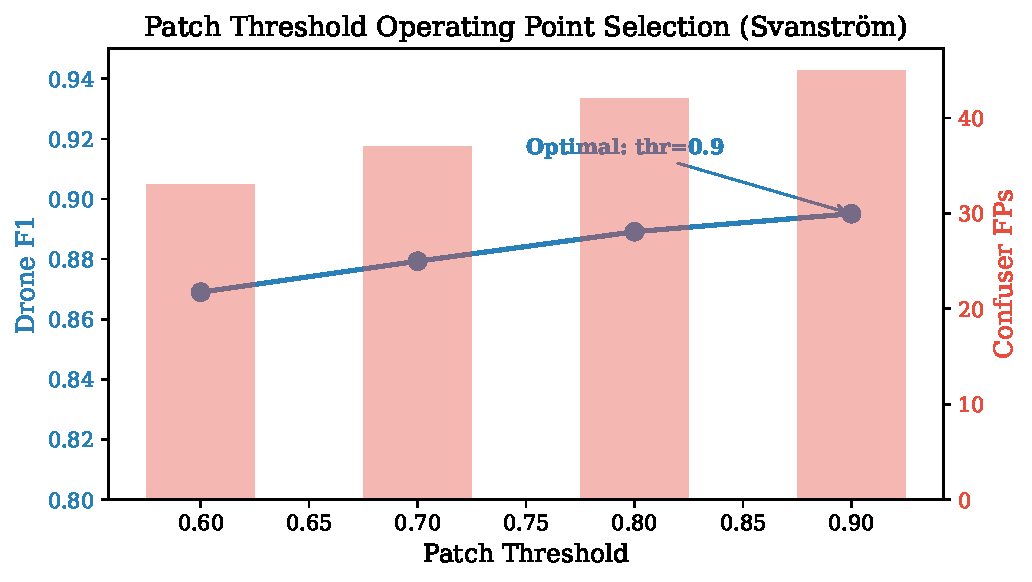
\includegraphics[width=0.85\textwidth]{fig6_3_threshold_sweep}
    \caption{Patch verifier threshold sweep on Svanstr\"om paired drones. The curve is monotone in the useful range. Production setting \texttt{patch\_thr=0.9} sits at the elbow where drone recall recovery saturates. Source: \textsc{Ledger}~\S7.}
    \label{fig:patch_sweep}
\end{figure}

The curve is monotone in the relevant range: every threshold bump from 0.5 to 0.9 recovers more drone recall than it costs in confuser FPs. At \texttt{patch\_thr=0.9}, the cascade still catches $\sim$63\% of S2's residual confuser FPs (45 vs 120) while costing only 4.0~pp drone F1 vs S2 (0.912 $\to$ 0.895). The production choice is therefore \texttt{patch\_thr=0.9}; above 0.9 is unmeasured but unlikely to be useful since the residual 14+31+0 confuser crops at 0.9 are already in the noise floor of the 1891-frame confuser slice.
% [source: ledger=patch-catch-below-bar; eval=svan_s3_sa32_thr08; run=(EVIDENCE_LEDGER sweep); config=svan_iop_1280_s9]

\subsection{Catch-Rate Audit}
\label{sec:patch_audit}

A dedicated audit (\texttt{eval/audit\_patch\_catch.py}; \textsc{Ledger}~\S6.1) measures per-bucket veto rates for the baseline + v2 verifier on Svanstr\"om at \texttt{imgsz=1280}, stride 9, conf 0.25 (3190 frames, 3130 detections). The audit is the diagnostic counterpart to the cumulative-suppression numbers: it reveals what the verifier is good at, what it is bad at, and where the remaining failure modes live.
% [source: ledger=patch-catch-below-bar; eval=patch_catch_v2_svan; run=(EVIDENCE_LEDGER sweep); config=patch_catch_svan_1280_s9]

\begin{table}[htbp]
    \centering
    \caption{Patch v2 catch and veto rates by bucket at \texttt{patch\_thr=0.5}. Drone TP veto is unwanted (lower is better); confuser catches are wanted (higher is better). Source: \textsc{Ledger}~\S6.1.}
    \label{tab:patch_audit}
    \begin{tabular}{lrcr}
        \toprule
        Bucket & N & Catch / veto rate & Median patch prob \\
        \midrule
        BIRD       & 807 & 0.638 catch & 0.904 \\
        AIRPLANE   & 532 & 0.517 catch & 0.540 \\
        HELICOPTER & 464 & 0.709 catch & 0.987 \\
        DRONE\_TP (unwanted veto) & 1248 & 0.054 veto & 0.000 \\
        DRONE\_FP (bonus catches) &   79 & 0.266 catch & 0.000 \\
        \bottomrule
    \end{tabular}
\end{table}

The audit identifies two patterns. The verifier is \emph{partially working}: helicopter catches are good (71\%), bird catches are mid (64\%), airplane catches are weak (52\%). All three are below the 90\% ``ceiling'' that would render the patch verifier the dominant suppression stage. The classifier remains the workhorse; the patch verifier is a useful but not decisive secondary stage. Independently, the drone-TP veto rate is only 5.4\%---the verifier is \emph{not} over-aggressive on drones at \texttt{patch\_thr=0.5}. Combined with the threshold sweep (\S\ref{sec:patch_threshold}), this is what makes \texttt{patch\_thr=0.9} a sound operating point: it lifts drone recall recovery to 0.869 without inflating the drone-TP veto into a recall problem.
% [source: ledger=patch-catch-below-bar; eval=patch_catch_v2_svan; run=(EVIDENCE_LEDGER sweep); config=patch_catch_svan_1280_s9]

\begin{figure}[htbp]
    \centering
    \fbox{\parbox{0.9\textwidth}{\centering\vspace{2cm}
        \textbf{[PLACEHOLDER: Fig 6.5 --- Patch verifier failure modes]} 6-up grid: three airplane crops the verifier classifies as \texttt{other} with softmax $\approx 0.5$ (uncertain), two bird crops correctly classified at $p_\text{bird} > 0.9$, and one drone-TP crop the verifier vetoes at $p_\text{airplane}=0.61$. Caption identifies the actionable retraining direction for a patch-verifier retrain.
        % [source: ledger=patch-catch-below-bar; eval=patch_catch_v2_svan; run=(EVIDENCE_LEDGER sweep); config=patch_catch_svan_1280_s9]
    \vspace{2cm}}}
    \caption{Representative patch-verifier outputs on Svanstr\"om-scale confuser crops. The airplane failure mode is genuine uncertainty in the softmax middle band, not a clean \texttt{other}-class abstention.}
    \label{fig:patch_failure_modes}
\end{figure}

\begin{figure}[htbp]
    \centering
    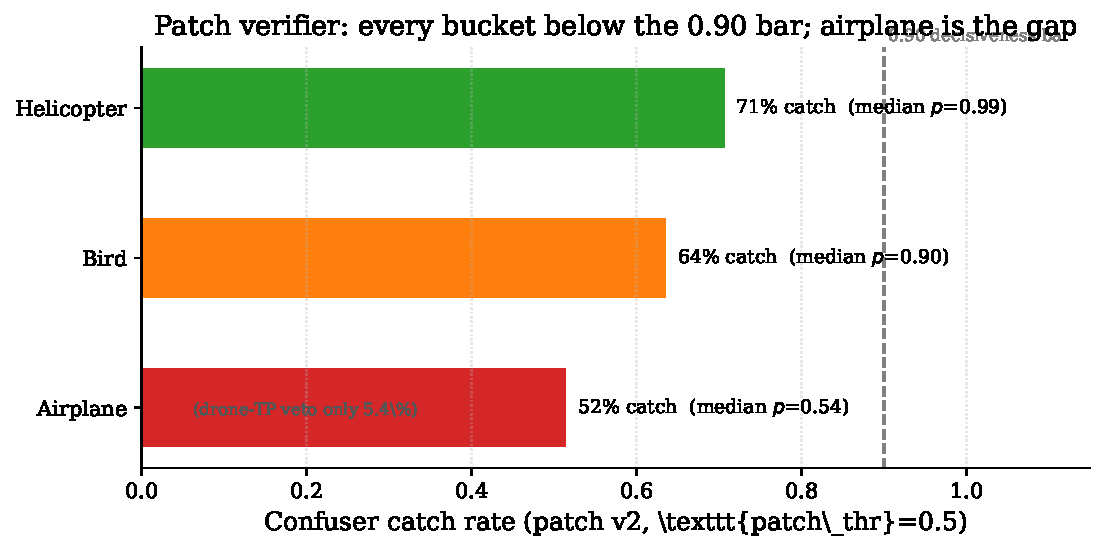
\includegraphics[width=0.8\textwidth]{fig8_patch_catchbar}
    \caption{Patch-verifier (v2) per-bucket confuser catch rate at \texttt{patch\_thr}=0.5, against the $0.90$ ``decisiveness'' bar. Helicopters ($71\%$) and birds ($64\%$) are mid; airplanes ($52\%$, median patch probability $0.540$ vs $0.90+$ for the others) are the actionable gap, and the drone-TP veto is only $5.4\%$. All three buckets sit below the bar, which is why the patch verifier is a useful-but-secondary stage --- and the motivation for the distilled \texttt{mlp\_v5} successor (\S\ref{sec:distill_verifier}). Source: \textsc{Ledger}~\S6.1.}
    % [source: ledger=patch-catch-below-bar; eval=patch_catch_v2_svan; run=(EVIDENCE_LEDGER sweep); config=patch_catch_svan_1280_s9]
    \label{fig:patch_catchbar}
\end{figure}

The airplane gap is the most actionable finding: 52\% catch with median patch probability 0.540 means the verifier is genuinely uncertain on a meaningful share of Svanstr\"om airplane crops, not just slightly under-confident. The v2 ``other'' class is a real OOD outlet (the verifier knows the crop is not one of its three confusers); the airplane misses are therefore not abstentions but \emph{active wrong classifications}, which makes them recoverable by retraining the verifier with the specific FP crops as confuser-class data. This is recorded as a planned next step in \texttt{path\_forward.md} \S3b.
% [source: ledger=patch-catch-below-bar; eval=patch_catch_v2_svan; run=(EVIDENCE_LEDGER sweep); config=patch_catch_svan_1280_s9]

\subsection{Distilled Feature-Space Verifier (\texttt{mlp\_v5})}
\label{sec:distill_verifier}

The catch-rate audit (\S\ref{sec:patch_audit}) exposes a structural limit of the MobileNetV3 patch verifier: it re-processes each detection crop as raw pixels with a network entirely separate from the detector, and on surfaces it was not trained against it abstains to \texttt{other} rather than discriminating. On SelCom CCTV, for instance, the patch verifier is bit-for-bit identical to the bare detector ($F1=0.591$, hallucination rate $0.071$ in both columns of Table~\ref{tab:distill_verifier}) because it has never seen CCTV-scale crops and votes \texttt{other} on all of them. This blind spot motivates a structurally different verifier.
% [source: ledger=patch-v2-neutral-selcom; eval=v5_selcom_patch; run=eval/eval_v4_vs_patch.py; config=selcom_iop_1280]

The \emph{distilled feature-space verifier} replaces pixel re-processing with feature reuse. Instead of a fresh CNN, a small multilayer perceptron consumes the RGB detector's own fused intermediate ROI features --- the \texttt{p3} (stride~8) and \texttt{p5} (stride~32) pyramid activations already computed for each candidate box, ROI-pooled to a 512-dimensional embedding plus 5 detection-metadata scalars ($517$ features total). These features were characterised with a dedicated \emph{Model MRI} tool (\texttt{python -m mri}; \S\ref{sec:reproducibility}) that hooks the detector's FPN layers, pools per-detection activations, and runs the separability analysis on the exact $32{,}931$-detection corpus (19{,}334 drone + 13{,}597 confuser) the shipped \texttt{mlp\_v5} was trained on. The analysis confirms the geometry the verifier exploits. A single linear discriminant separates drone from confuser at $\approx 95\%$ train accuracy (Figure~\ref{fig:mri_stats}a), while an unsupervised PCA projection of the same features shows near-zero cluster separation (silhouette $0.067$). The signal is therefore real but lives in a supervised discriminant subspace, which is why a trained classifier, not a distance threshold, is required. The single most discriminative feature is a \texttt{p5} channel (ANOVA $F=42{,}346$), almost $3\times$ stronger than the best \texttt{p3} channel and $4\times$ the detection-confidence scalar (which ranks only 6th, Figure~\ref{fig:mri_stats}b): the verifier reads the detector's semantic activations, not merely its score.
% [source: ledger=v5-lda-separability; eval=distill_cv_mlp; run=mri/cli.py; cache=mri/docs/mlp_v5_report_regen.md; config=distill_cv_5fold]
% [source: ledger=mri-v5-report-regen; eval=distill_cv_mlp; run=mri/cli.py; cache=mri/results/v5_report_regen/stats.json; config=distill_cv_5fold]

\begin{figure}[htbp]
    \centering
    \begin{subfigure}{0.6\textwidth}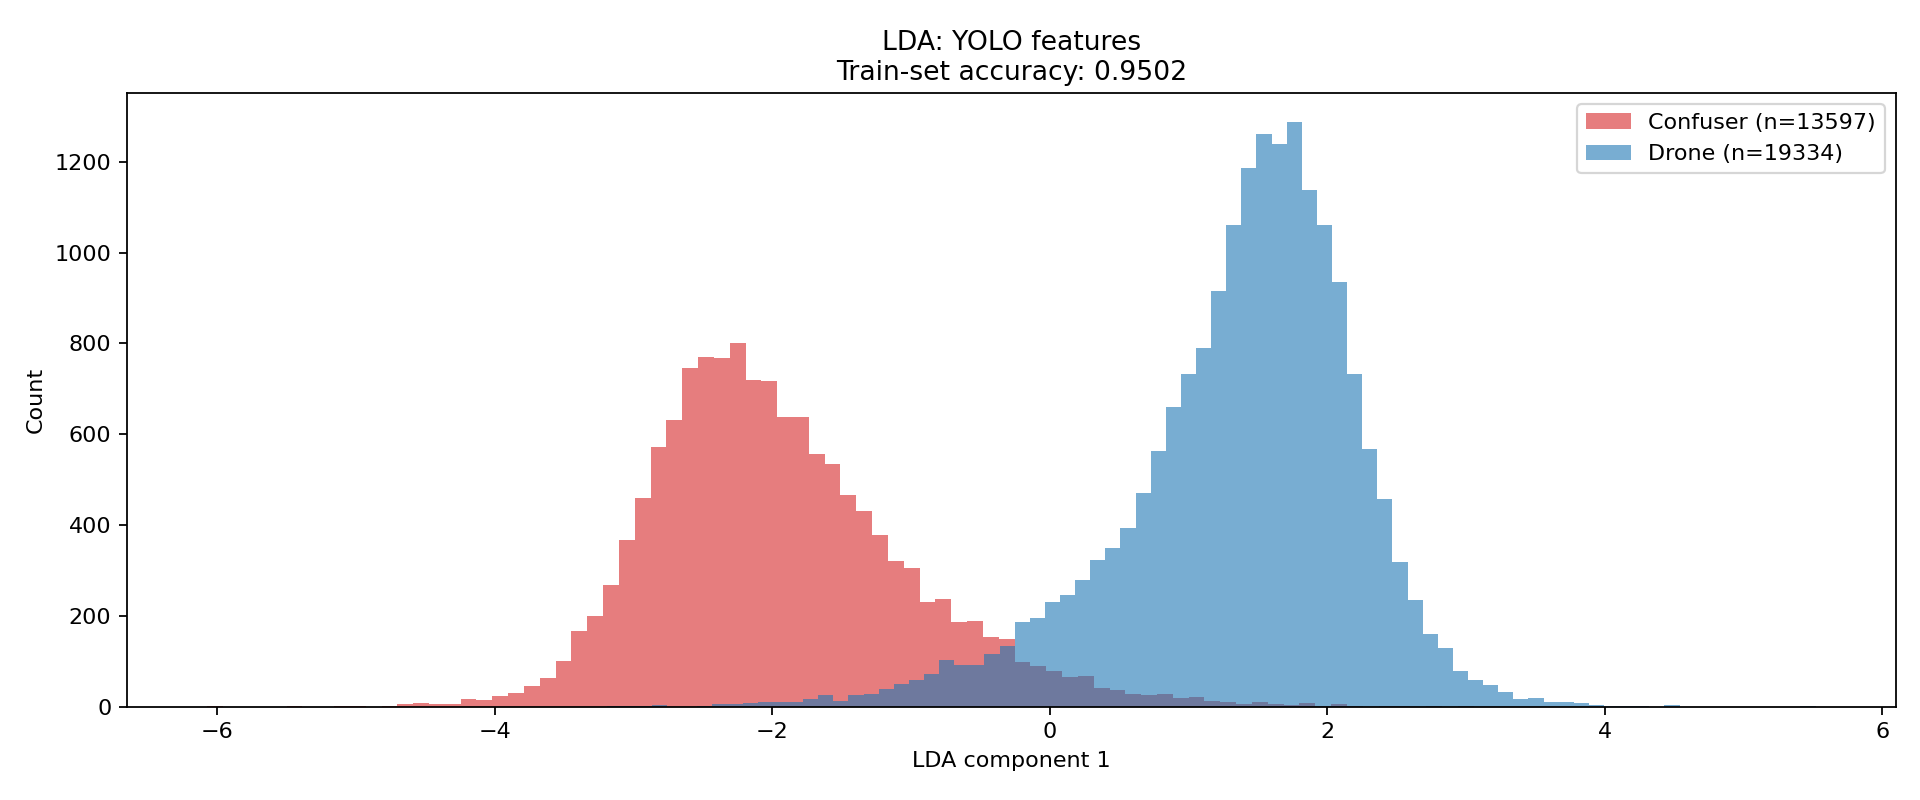
\includegraphics[width=\textwidth]{fig8_mri_lda}\caption{}\end{subfigure}
    \begin{subfigure}{0.39\textwidth}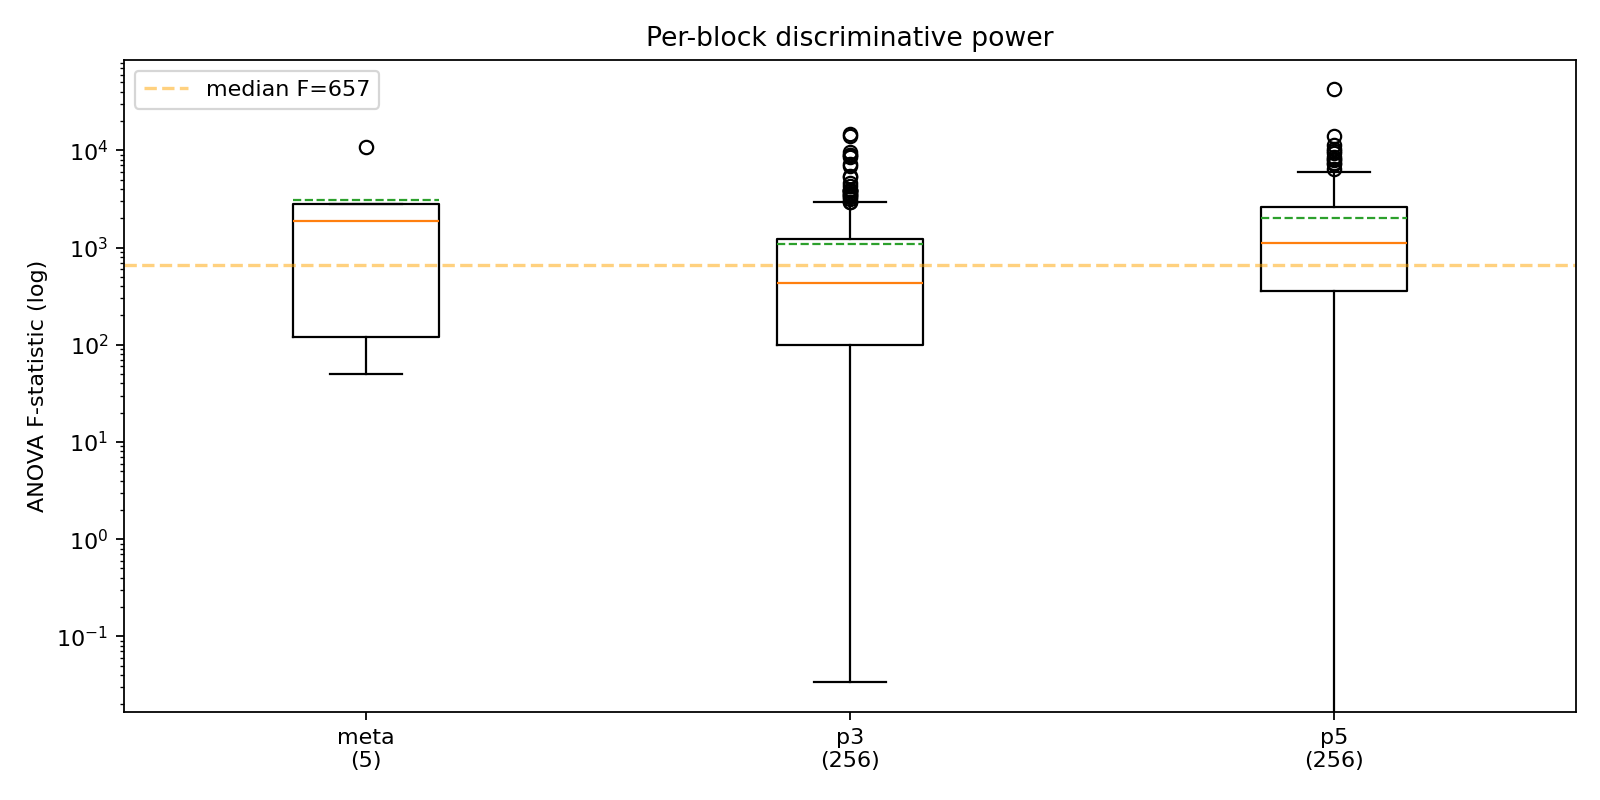
\includegraphics[width=\textwidth]{fig8_mri_anova}\caption{}\end{subfigure}
    \caption{Model MRI of the FT4 detector's fused \texttt{p3}+\texttt{p5} ROI features on the shipped $32{,}931$-detection V5 corpus. (a) The linear-discriminant projection separates drone (blue) from confuser (red) into two cleanly-resolved peaks at $\approx 95\%$ single-threshold accuracy. (b) Per-block ANOVA $F$-statistic: \texttt{p5} is the dominant discriminative layer (max $F=42{,}346$, mean $2{,}006$), ahead of \texttt{p3} and the detection metadata. Source: Model MRI regeneration, \textsc{Ledger}~mri-v5-report-regen.}
    % [source: ledger=mri-v5-report-regen; eval=distill_cv_mlp; run=mri/cli.py; cache=mri/results/v5_report_regen/stats.json; config=distill_cv_5fold]
    \label{fig:mri_stats}
\end{figure}
% [source: ledger=v5-lda-separability; eval=distill_cv_mlp; run=eval/overnight_confuser_distill.py; config=distill_cv_5fold]
% [source: ledger=embedding-distillation-cv; eval=distill_cv_mlp; run=eval/overnight_confuser_distill.py; config=distill_cv_5fold]

\begin{table}[htbp]
    \centering
    \caption{Distilled feature-space verifier (\texttt{mlp\_v5}) vs the MobileNetV3 patch verifier (v2), both on top of the FT4 RGB detector (\texttt{Yolo26n\_selcom\_confuser\_ft4\_1280}). $F1$ is drone-class (IoP@0.5 on Svanstr\"om/SelCom, IoU@0.5 on Anti-UAV/\texttt{rgb\_dataset}); \emph{halluc} is the confuser hallucination rate (lower is better). The confuser-only surface has no drone GT, so only the hallucination rate is defined. \texttt{mlp\_v5} wins on Svanstr\"om, SelCom, and confuser-only; ties on saturated Anti-UAV; and regresses on the photo-style \texttt{rgb\_dataset} split. Source: \textsc{Ledger} (v5-beats-patch, v5-rgbds-ceiling).}
    \label{tab:distill_verifier}
    \begin{tabular}{lcccccc}
        \toprule
        & \multicolumn{3}{c}{Drone $F1$} & \multicolumn{3}{c}{Halluc. rate} \\
        \cmidrule(lr){2-4} \cmidrule(lr){5-7}
        Surface & bare FT4 & + patch v2 & + \texttt{mlp\_v5} & bare & patch v2 & \texttt{mlp\_v5} \\
        \midrule
        Svanstr\"om (IoP@0.5)      & 0.596 & 0.768 & \textbf{0.869} & 0.470 & 0.163 & \textbf{0.037} \\
        Anti-UAV (IoU@0.5)         & 0.986 & 0.986 & 0.985          & 0.011 & 0.011 & \textbf{0.010} \\
        SelCom CCTV (IoP@0.5)      & 0.591 & 0.591 & \textbf{0.607} & 0.071 & 0.071 & \textbf{0.019} \\
        \texttt{rgb\_dataset} (IoU)& \textbf{0.929} & 0.904 & 0.792 & 0.028 & 0.026 & \textbf{0.010} \\
        confuser-only              & ---   & ---   & ---            & 0.317 & 0.107 & \textbf{0.008} \\
        \bottomrule
    \end{tabular}
\end{table}

\begin{figure}[htbp]
    \centering
    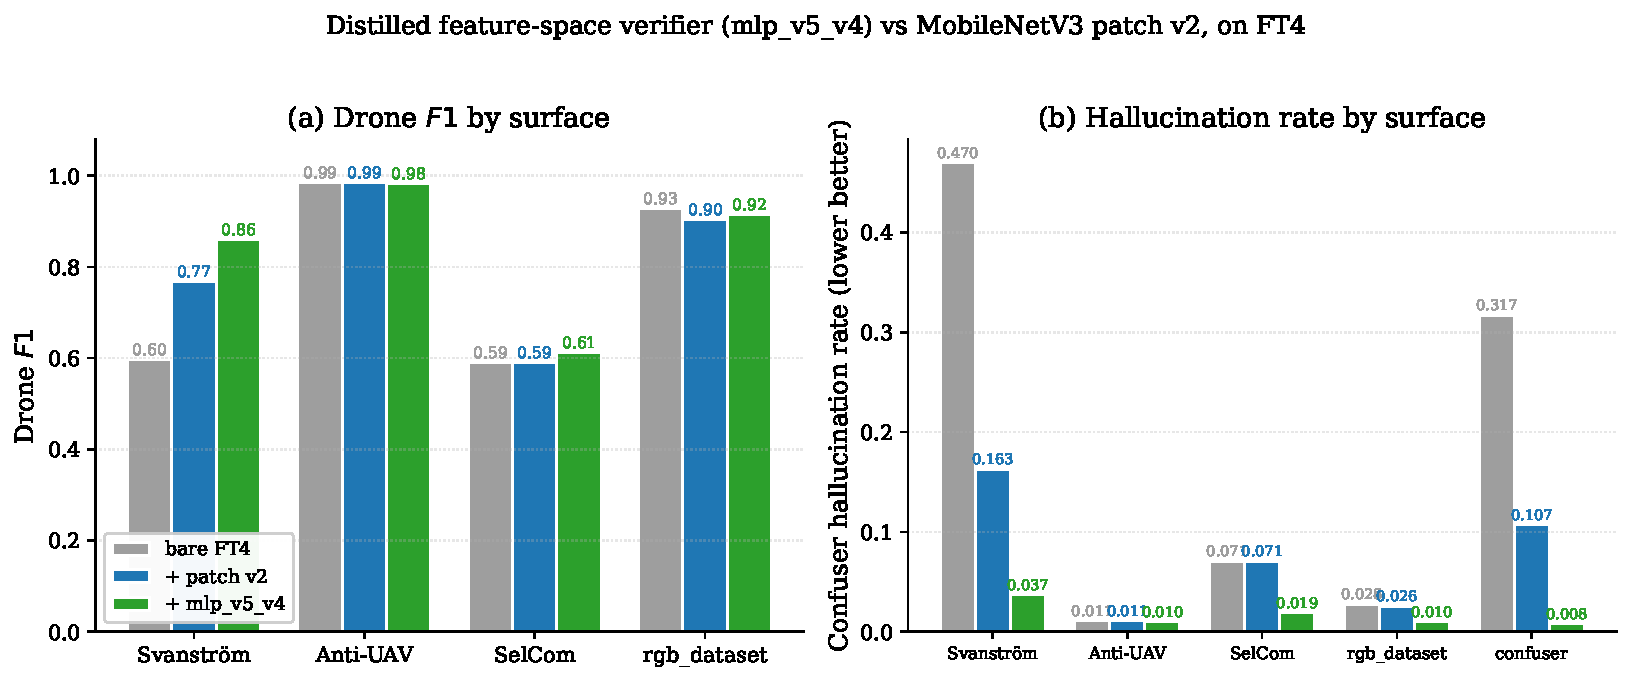
\includegraphics[width=0.95\textwidth]{fig8_distill_verifier}
    \caption{Distilled feature-space verifier (\texttt{mlp\_v5}, green) vs the MobileNetV3 patch verifier (v2, blue) and the bare FT4 detector (grey), per evaluation surface. (a) Drone $F1$: \texttt{mlp\_v5} wins on Svanstr\"om, edges SelCom, ties saturated Anti-UAV, and regresses on the photo-style \texttt{rgb\_dataset} split. (b) Confuser hallucination rate (lower is better): \texttt{mlp\_v5} is lowest on every surface, most dramatically on Svanstr\"om ($0.470\to0.037$) and the confuser-only set ($0.317\to0.008$). Generated from \texttt{knowledge/evals.csv}. Source: \textsc{Ledger}~v5-beats-patch, v5-rgbds-ceiling.}
    % [source: ledger=v5-beats-patch; eval=v5_svan_mlp; run=eval/eval_v4_vs_patch.py; config=svan_iop_1280_s9]
    \label{fig:distill_verifier_bar}
\end{figure}

The verifier beats the patch verifier on three of the five surfaces (Figure~\ref{fig:distill_verifier_bar}). On Svanstr\"om it raises drone $F1$ from $0.768$ to $0.869$ (a $\sim 10$-pp gain) while cutting the hallucination rate from $0.163$ to $0.037$; on SelCom it gains $1.5$~pp $F1$ over the bare detector where the patch verifier gains nothing; and on the confuser-only surface it drops the hallucination rate from $0.107$ (patch v2) to $0.008$, a $13\times$ reduction. It ties the patch verifier on the saturated Anti-UAV surface. Because it reuses features the detector has already computed rather than running a second network over crop pixels, it is $46$--$72\times$ faster per detection at an estimated $1$--$4\%$ pipeline overhead, cheap enough to run \emph{per frame} rather than alert-gated. Alert-gating it would save under $0.2$~ms per frame but cost $4.0$~pp of Svanstr\"om $F1$, so per-frame operation is the correct deployment choice.
% [source: ledger=v5-beats-patch; eval=v5_confuser_mlp; run=eval/eval_v4_vs_patch.py; config=confuser_test_640]
% [source: ledger=v5-ship-per-frame; eval=v5_svan_mlp; run=eval/eval_v4_vs_patch.py; config=svan_iop_1280_s9]

The carve-out is the photo-style \texttt{rgb\_dataset} held-out split, where the verifier regresses to $F1=0.792$ against the patch verifier's $0.904$ ($-11$~pp), driven by a recall collapse (drone $R$ $0.896$ bare $\to 0.664$). This is a structural recall ceiling, not a tuning problem. A threshold sweep, a Svanstr\"om-weight rebalance, and a $14{,}500$-drone coverage boost all failed to close it (the coverage boost was net-negative, $-3$~pp recall), which points to a train/test distribution mismatch between the verifier's confuser-rich training surfaces and the photo-style held-out split. The distilled \texttt{mlp\_v5} verifier therefore \emph{supersedes} the v2 patch verifier as the production confuser verifier (\textsc{Ledger}~v5-ship-per-frame): it wins on every confuser-rich surface (Svanstr\"om, SelCom, the OOD zoo) and runs per-frame at a fraction of the cost. Two limitations are reported honestly rather than hidden. First, on the photo-style \texttt{rgb\_dataset} held-out split the distilled verifier still trails the patch verifier ($F1=0.792$ vs $0.904$), a structural recall ceiling traceable to a train/test distribution mismatch; this is the one surface where the successor has not yet caught up. Second, every surface in Table~\ref{tab:distill_verifier} uses the FT4 detector as the feature source, so the magnitude of the gains on the baseline detector that drives the cascade elsewhere is an open item. Neither limitation reverses the supersession on the confuser-rich surfaces the cascade exists to handle. The recall ceiling itself is diagnosed in \S\ref{sec:mlp_recall_drop} as an out-of-distribution coverage gap rather than an irreducible structural limit; however, no runtime fix closes it without cost, so the verifier is shipped at its full-veto operating point and the regression is recorded as a still-image carve-out --- benign for the deployment target, where frame-level recall on video is unaffected.
% [source: ledger=v5-rgbds-ceiling; eval=v5_rgbds_mlp; run=eval/eval_v4_vs_patch.py; config=rgb_dataset_iou_640]
% [source: ledger=v5-rgbds-ceiling; eval=v52_rgbds_remine; run=eval_distill_v5_remine_rgb; config=rgb_dataset_iou_640]

\paragraph{What the verifier sees.}
The abstract separability becomes concrete when the top discriminative neurons are rendered spatially on real detections (Figure~\ref{fig:mri_activation}). On a drone, the \texttt{p3} activation locks tightly onto the airframe and the \texttt{p5} activation forms a single clean semantic blob centred on the object; on a confuser the same neurons fire in a diffuse, fragmented pattern smeared across background structure. The MLP separates these two activation signatures, which is why a $517$-feature near-linear boundary suffices: it reaches a 5-fold cross-validation $F1$ of $0.9857\pm0.0004$ on the shipped corpus and, out of fold, rejects $97\%$ of confuser detections while retaining $98.9\%$ of true drones. These activation maps were produced by the same Model MRI tool, which doubles as an auditing instrument: regenerating the V5 evidence on the \emph{shipped} corpus surfaced and corrected two stale figures in an earlier report (the dominant discriminator is the \texttt{p5} channel above, not the confidence score as originally claimed).
% [source: ledger=mri-v5-report-regen; eval=distill_cv_mlp; run=mri/cli.py; cache=mri/results/v5_report_regen/stats.json; config=distill_cv_5fold]

\begin{figure}[htbp]
    \centering
    \begin{subfigure}{\textwidth}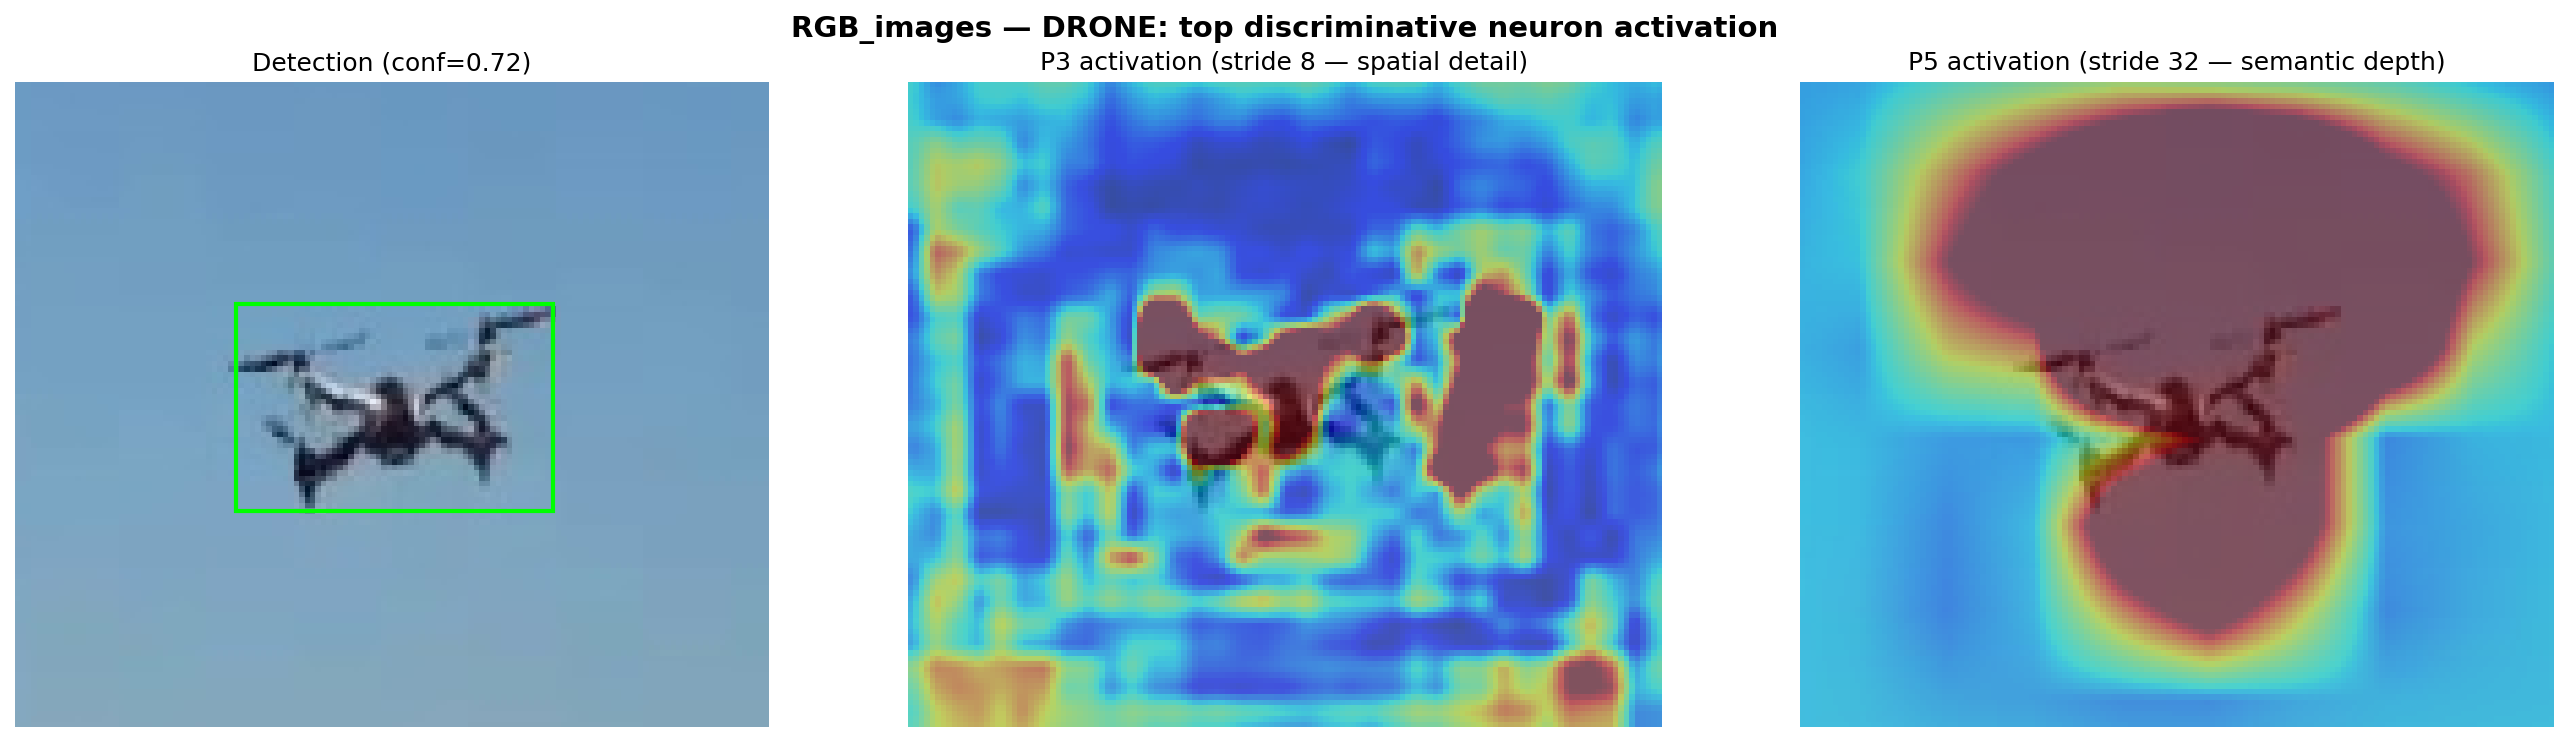
\includegraphics[width=\textwidth]{fig8_mri_act_drone}\caption{Drone (Svanstr\"om, conf$=0.72$)}\end{subfigure}
    \\[4pt]
    \begin{subfigure}{\textwidth}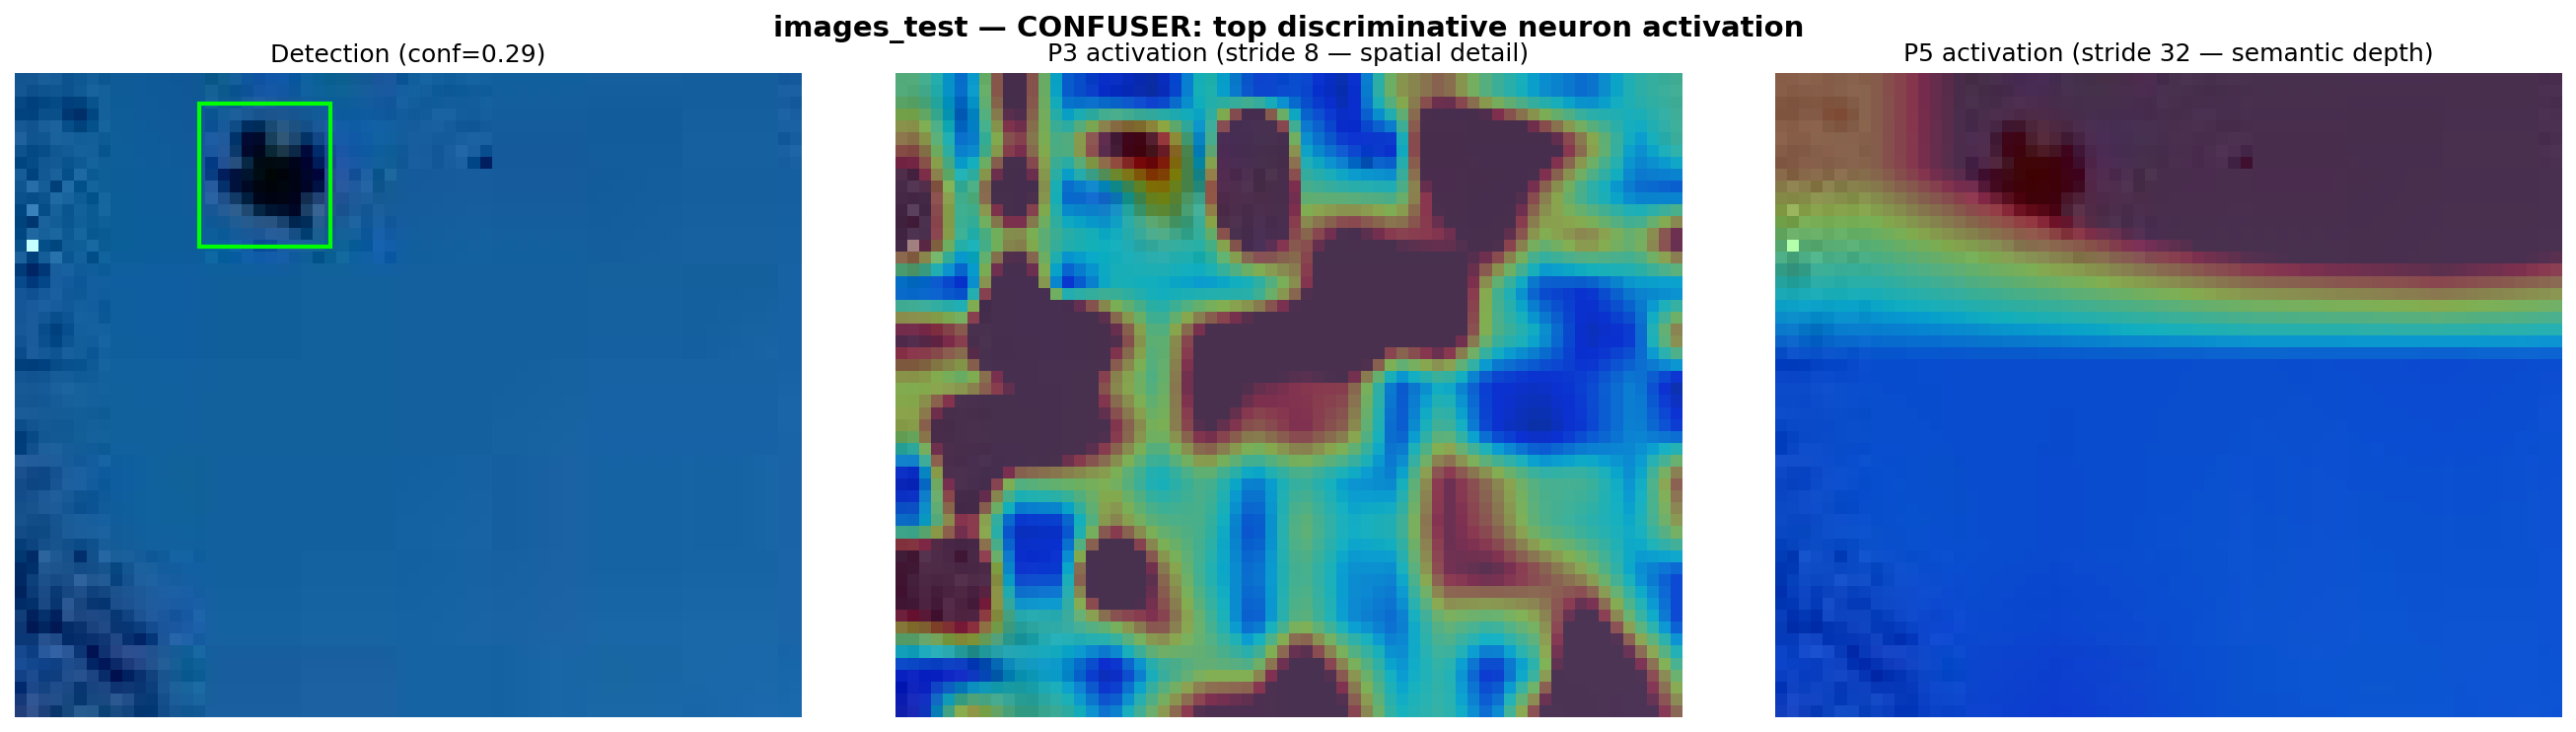
\includegraphics[width=\textwidth]{fig8_mri_act_confuser}\caption{Confuser (\texttt{rgb\_confusers} test, conf$=0.29$)}\end{subfigure}
    \caption{Model MRI spatial ``brain scan'' of the top discriminative neurons. Each row: the detection crop, the \texttt{p3} activation (stride~8, fine spatial detail), and the \texttt{p5} activation (stride~32, semantic depth). On the drone (a) \texttt{p3} binds to the airframe and \texttt{p5} forms a centred semantic blob; on the confuser (b) the same neurons fire diffusely across background structure. This activation-signature difference is what the distilled verifier reads. Source: Model MRI live scan, \textsc{Ledger}~mri-v5-report-regen.}
    \label{fig:mri_activation}
\end{figure}

\subsection{Diagnosing the Recall Drop: an Out-of-Distribution Coverage Gap}
\label{sec:mlp_recall_drop}

The recall regression on the photo-style \texttt{rgb\_dataset} split (Table~\ref{tab:distill_verifier}: drone $R$ $0.896\to0.664$) was reported above as a ``structural recall ceiling'' without a mechanism. The same Model MRI statistics that explain what the verifier reads can also localise \emph{why} it vetoes real drones. We take the cached $517$-feature detections, keep only those that match a ground-truth drone, and split them into the ones the verifier keeps (MLP probability $\geq 0.25$) and the ones it falsely vetoes (the recall loss), then run the separability analysis on the two groups. The falsely-vetoed drones are not low-confidence --- the confidence-scalar mean is identical between the two groups ($\Delta=0.000$), which refutes the obvious hypothesis that the verifier simply kills marginal detections. What distinguishes them is that they are \emph{smaller} (mean \texttt{log\_area} $-0.180$ vetoed vs $-0.075$ kept; $\Delta+0.188$ on Svanstr\"om) and carry a distinct deep-feature signature: the top discriminators are individual \texttt{p3} and \texttt{p5} neurons that reach a single-neuron AUROC of $\approx 0.89$. We report the per-neuron AUROC, not the linear-discriminant separability, as the honest signal: with $517$ features and on the order of $770$ samples an LDA separates almost anything, so its near-perfect accuracy here is a high-dimensional artefact rather than evidence.
% [source: ledger=mlp-v5-recall-drop-is-ood-coverage; eval=clf_own_holdout; run=eval/diagnose_mlp_recall_drop.py; cache=eval/results/_offline_pipeline/cache; config=clf_own_holdout]

The decisive measurement is whether these vetoed drones look like confusers. In the standardised feature space they sit \emph{farther} from the confuser distribution than the kept drones (centroid distance $16.48$ vs $11.05$) and are at least as separable from confusers (mean top-$20$ AUROC $0.876$ vs $0.862$); they are also far from the verifier's training-drone cluster (centroid distance $15.37$). The vetoed drones are therefore an out-of-distribution outlier cluster --- small, atypical real drones that are far from confusers \emph{and} far from the drones the MLP was trained on. The verifier rejects them because they do not resemble its training drones, not because they resemble birds. This reframes the carve-out: the recall drop is consistent with a coverage gap rather than a structural drone/confuser overlap, which suggests it is recoverable in principle (the no-retrain remedy and its limits are weighed next).
% [source: ledger=mlp-v5-recall-drop-is-ood-coverage; eval=clf_own_holdout; run=eval/_veto_vs_confuser.py; cache=eval/results/_offline_pipeline/cache; config=clf_own_holdout]

\paragraph{A fail-open gate --- promising, but not adopted.}
The diagnosis prescribes its own remedy. Because the vetoed drones are far from confusers while the correctly-vetoed confusers are close to them, a verifier can be made recall-first by \emph{abstaining} --- keeping a detection it would otherwise veto whenever that detection is out-of-distribution relative to the confuser set, measured as a $k$-nearest-neighbour distance to the confuser distribution exceeding a threshold $\tau$. The verifier only vetoes when it is confidently near a confuser. On the falsely-vetoed real drones (which we want to release) versus the correctly-vetoed confusers (which we want to keep vetoed), the OOD-from-confuser distances separate cleanly (median $34.4$ for vetoed drones vs $9.8$ for vetoed confusers), and the threshold sets the trade (Table~\ref{tab:failopen}, Figures~\ref{fig:failopen_hist}--\ref{fig:failopen_tradeoff}). At a tolerated $5\%$ confuser leak the gate recovers $91.3\%$ of the falsely-vetoed drones ($157$ of $172$); at $10\%$ it recovers all of them. In absolute terms a $5\%$ leak is roughly $10$ extra confuser false positives across $2{,}633$ images in exchange for restoring drone recall from $\approx 0.69$ back to $\approx 0.89$. The gate needs no retraining and matches the diagnosis exactly: veto only near confusers, abstain on OOD. The deployment engine already exposes the hook (\texttt{\_mlp\_gate\_open} in \texttt{ir\_gui/pyside\_engine.py}). The honest limit is that the abstain rule is calibrated against the \emph{known} confuser set. The irreducible $\approx 9\%$ tail of vetoed drones that genuinely overlap confusers cannot be recovered this way --- a targeted drone-diversity re-mine would be needed, and an untargeted re-mine has already been shown to fail. By the same logic, a genuinely novel confuser that lands far from the calibration set would be passed rather than vetoed. On the photo-style \texttt{rgb\_dataset} split, then, the gate cleanly trades a handful of confuser false positives for the lost recall.
% [source: ledger=mlp-v5-recall-drop-is-ood-coverage; eval=clf_own_holdout; run=eval/test_failopen_verifier.py; cache=eval/results/_offline_pipeline/cache; config=clf_own_holdout]

\paragraph{Why it is not adopted, and the decision.}
This recovery does not generalise off the photo-style surface. The same gate, calibrated on the \texttt{rgb\_confusers} set, \emph{backfires} on cluttered Svanstr\"om: because Svanstr\"om's bird and edge clutter is itself out-of-distribution relative to the calibration confusers, the abstain rule wrongly releases it, collapsing precision from $0.887$ (full veto) to $0.631$ at matched recall.
% [source: ledger=verifier-recall-precision-decision; eval=clf_own_holdout; run=eval/eval_failopen_prepost.py; cache=eval/results/_offline_pipeline/cache; config=clf_own_holdout]
Expanding the confuser reference to include held-out Svanstr\"om clutter recovers only about half of the lost precision ($0.486 \to 0.611$ at recall $0.90$, against the full-veto $0.884$; Figure~\ref{fig:failopen_expanded}), confirming the backfire is part calibration artefact and part a genuine recall/precision trade rooted in real drone--clutter overlap.
% [source: ledger=verifier-recall-precision-decision; run=eval/failopen_expanded_ref.py; cache=docs/analysis/images/failopen_expanded_ref_svan.png; config=clf_own_holdout]
Two further runtime remedies also fail. Up-weighting the under-scored drones in the existing training pool is a no-op: only $43$ of $19{,}334$ training drones are under-scored, so the out-of-distribution drones are \emph{absent} from training and re-weighting has nothing to act on. And $2$-of-$3$ temporal voting cannot recover the loss, because the veto is \emph{systematic} across frames rather than a transient flicker ($\Delta R = -0.008$ on the photo-style frames); on true video the full-veto verifier's frame-level recall is already $\approx 1.0$, so there is nothing to recover there.
% [source: ledger=verifier-recall-precision-decision; run=eval/retrain_v5_targeted.py; cache=eval/results/_v5_retargeted; config=clf_own_holdout]
% [source: ledger=verifier-recall-precision-decision; run=eval/temporal_ablation.py; cache=eval/results/_overnight_ablation_full/cache; config=clf_own_holdout]
The carve-out is therefore retained rather than patched. It is benign for the deployment target: on video, frame-level alert recall with the full-veto verifier is $\approx 1.0$ (a drone seen across consecutive frames survives even when individual boxes are vetoed), so the recall drop is confined to single-frame, photo-style benchmarks (\texttt{rgb\_dataset}, frame-level $R\ 0.93 \to 0.84$). Every runtime fix either backfires on the cluttered surfaces the verifier exists to clean (fail-open), is a no-op (re-weighting), or cannot apply (temporal) --- each adding complexity for a non-deployment-target benefit. The production verifier is shipped at its full-veto operating point; the residual recall gap is recorded as a still-image carve-out whose only frontier-moving remedy is closing the out-of-distribution coverage gap with diverse small-drone training data, the same lever that made the IR verifier recall-safe (\S\ref{sec:ir_xmodal_verifier}). The fail-open gate and the expanded-reference calibration remain on file as recall-first options for single-frame deployments where a false alarm is cheaper than a miss.
% [source: ledger=verifier-recall-precision-decision; eval=clf_own_holdout; run=eval/eval_failopen_prepost.py; cache=eval/results/_overnight_ablation_full/cache; config=clf_own_holdout]

\begin{figure}[htbp]
    \centering
    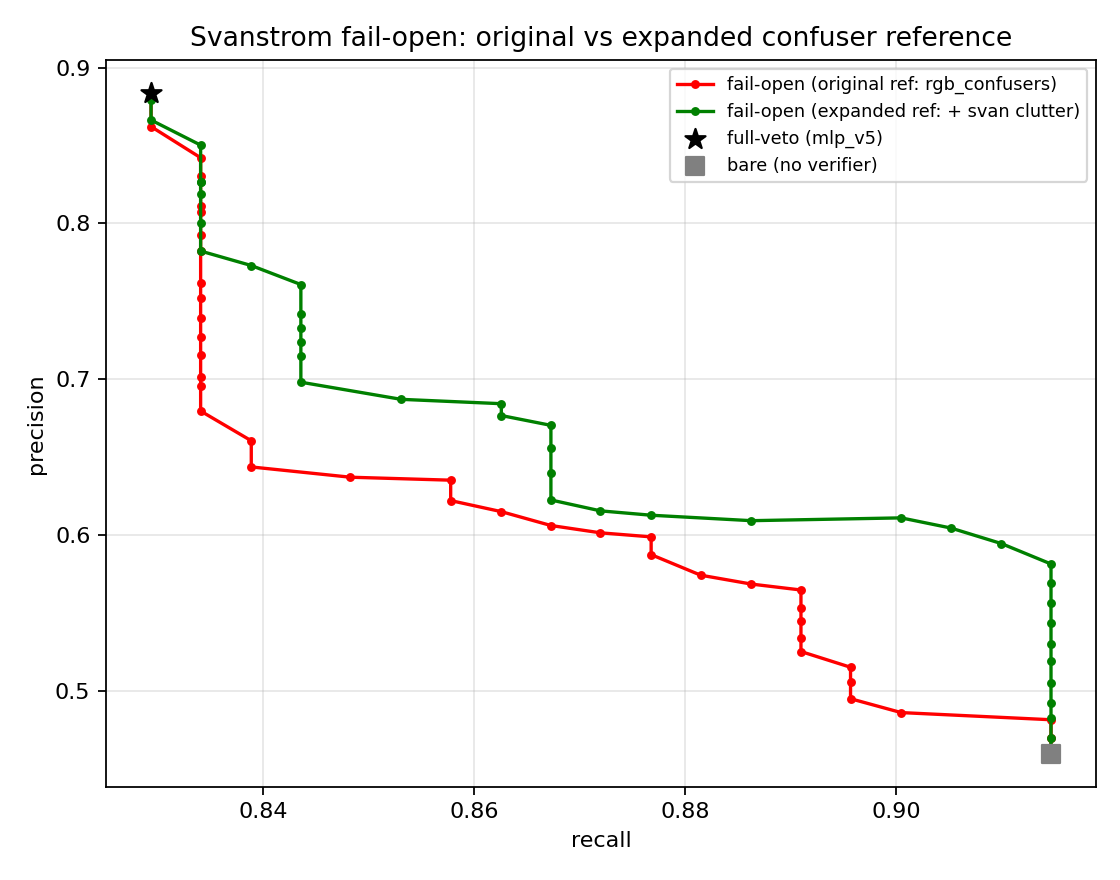
\includegraphics[width=0.7\textwidth]{fig8_failopen_expanded}
    \caption{Why fail-open is not adopted: the recall/precision frontier on Svanstr\"om for the fail-open gate with the original \texttt{rgb\_confusers} reference (red) versus a reference expanded with held-out Svanstr\"om clutter (green), against the full-veto operating point (star) and the bare detector (square). Expanding the reference recovers roughly half the precision the original-reference gate gives up, but the full-veto point still dominates at high recall --- the trade is partly calibration and partly fundamental. Source: \textsc{Ledger}~verifier-recall-precision-decision; \texttt{eval/failopen\_expanded\_ref.py}.}
    \label{fig:failopen_expanded}
\end{figure}

\begin{table}[htbp]
    \centering
    \caption{Fail-open (OOD-abstain) recovery of falsely-vetoed real drones, as a function of the tolerated confuser leak. The threshold $\tau$ is on the kNN distance to the confuser distribution. Source: \textsc{Ledger}~mlp-v5-recall-drop-is-ood-coverage; \texttt{eval/test\_failopen\_verifier.py}.}
    \label{tab:failopen}
    \begin{tabular}{ccc}
        \toprule
        tolerated confuser leak & $\tau$ & falsely-vetoed drones recovered \\
        \midrule
        $\leq 2\%$  & 21.9 & $83.1\%$ ($143/172$) \\
        $\leq 5\%$  & 19.3 & $\mathbf{91.3\%}$ ($157/172$) \\
        $\leq 10\%$ & 15.8 & $100\%$ ($172/172$) \\
        \bottomrule
    \end{tabular}
\end{table}

\begin{figure}[htbp]
    \centering
    \begin{subfigure}{0.48\textwidth}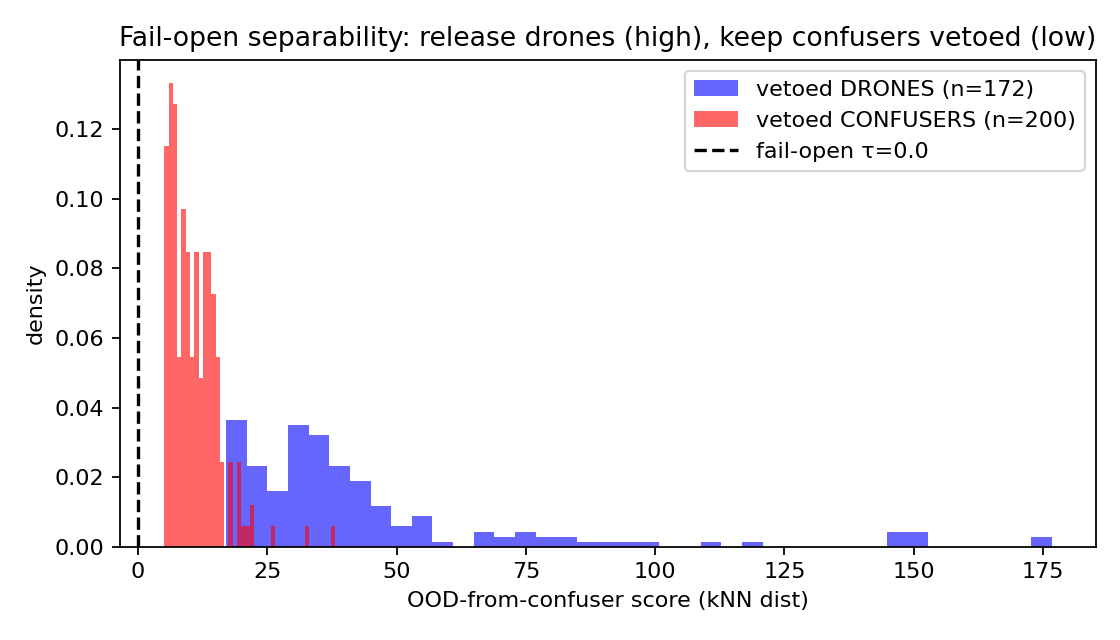
\includegraphics[width=\textwidth]{fig8_failopen_hist}\caption{}\label{fig:failopen_hist}\end{subfigure}
    \hfill
    \begin{subfigure}{0.48\textwidth}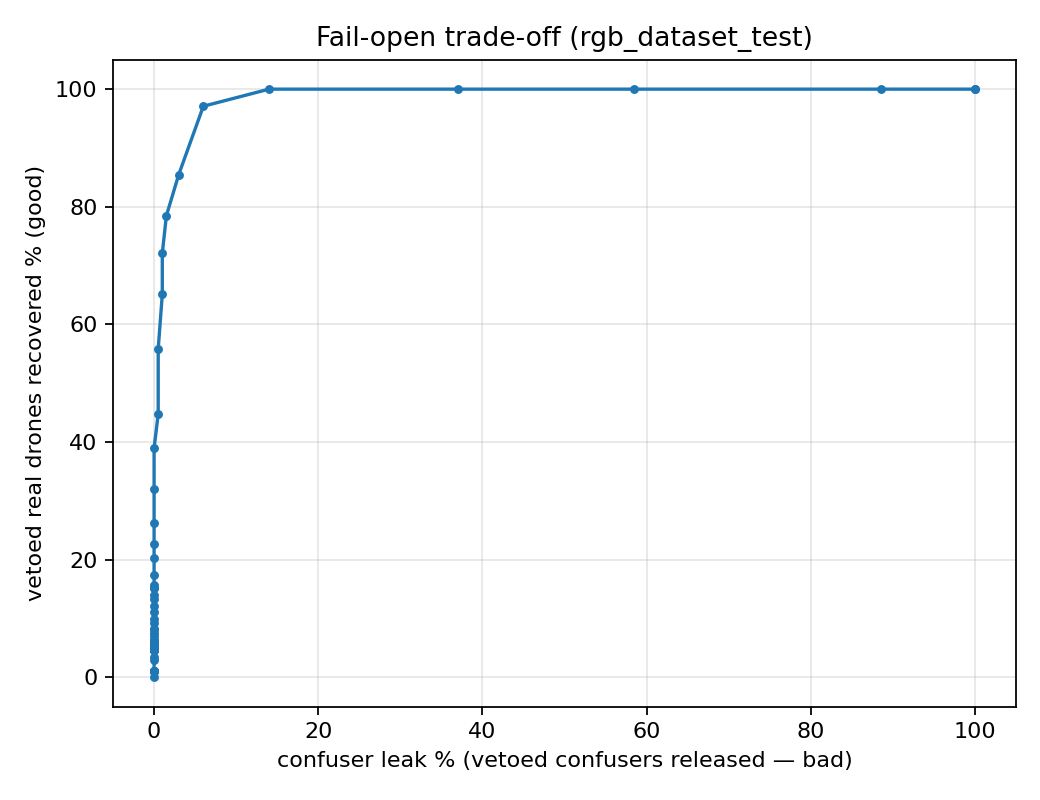
\includegraphics[width=\textwidth]{fig8_failopen_tradeoff}\caption{}\label{fig:failopen_tradeoff}\end{subfigure}
    \\[4pt]
    \begin{subfigure}{0.6\textwidth}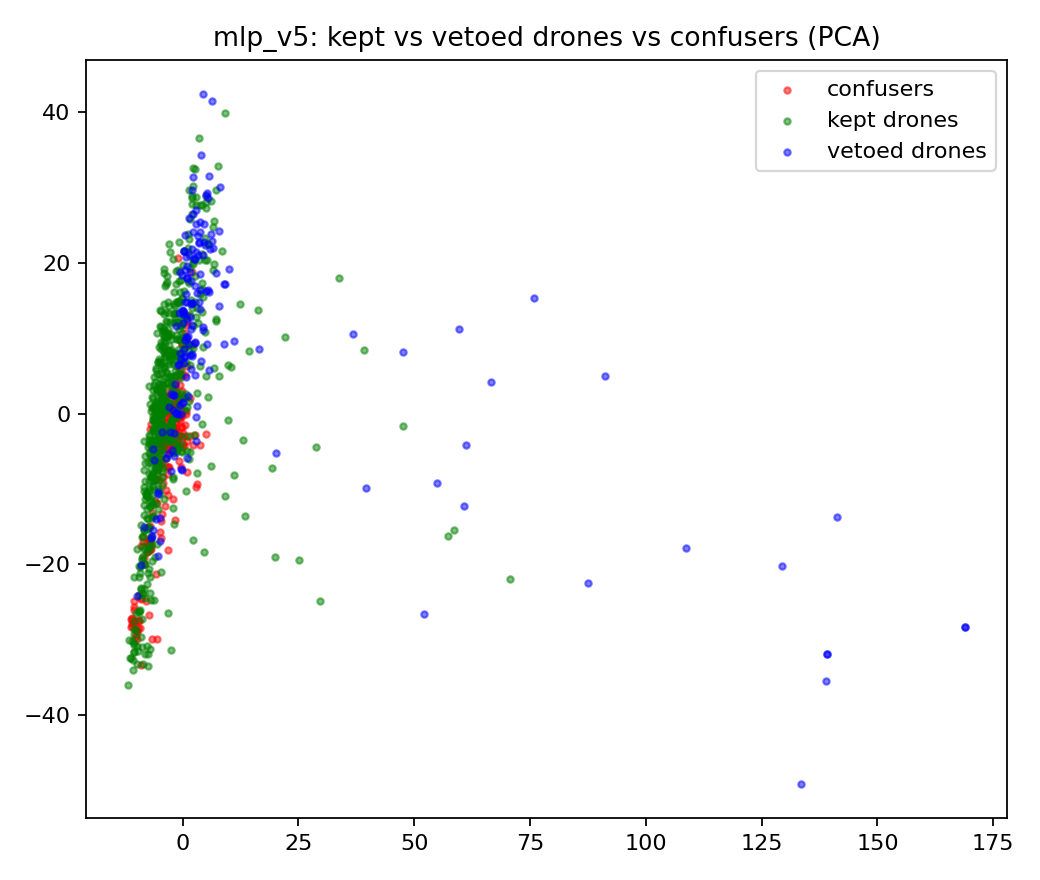
\includegraphics[width=\textwidth]{fig8_failopen_pca}\caption{}\label{fig:failopen_pca}\end{subfigure}
    \caption{Fail-open diagnosis and fix. (a) OOD-from-confuser distance: falsely-vetoed real drones (median $34.4$) separate cleanly from correctly-vetoed confusers (median $9.8$). (b) Recovery vs tolerated confuser leak: $91.3\%$ of vetoed drones recovered at $5\%$ leak, $100\%$ at $10\%$. (c) PCA of the standardised feature space showing the vetoed-drone cluster sitting away from both the confuser and the kept-drone distributions. Source: \textsc{Ledger}~mlp-v5-recall-drop-is-ood-coverage; \texttt{eval/diagnose\_mlp\_recall\_drop.py}, \texttt{eval/test\_failopen\_verifier.py}.}
    % [source: ledger=mlp-v5-recall-drop-is-ood-coverage; eval=clf_own_holdout; run=eval/test_failopen_verifier.py; cache=eval/results/_offline_pipeline/cache; config=clf_own_holdout]
    \label{fig:failopen}
\end{figure}

This closes the carve-out as far as the evidence allows: the recall ceiling reported in Table~\ref{tab:distill_verifier} is an OOD coverage gap, the gap is mechanistically localised (small, atypical drones far from confusers), and a no-retrain gate recovers $91$--$100\%$ of it at a small, quantified false-positive cost. The same diagnostic pattern recovered the deployable thermal IR verifier (\S\ref{sec:grayscale_verifier}): in both modalities the MRI statistics did not merely explain a failure but localised it and prescribed the recall-safe fix.
% [source: ledger=mlp-v5-recall-drop-is-ood-coverage; eval=clf_own_holdout; run=eval/diagnose_mlp_recall_drop.py; cache=eval/results/_offline_pipeline/cache; config=clf_own_holdout]

% ======================================================================
% CHAPTER 5 — DATASET CURATION AND HUMAN-IN-THE-LOOP
% ======================================================================
\chapter{Dataset Curation and Human-in-the-Loop}
\label{ch:hitl}

The IR detector described in the previous chapter was not trained once on a fixed corpus. It was co-developed with its training dataset across five numbered revisions, each driven by the model's own failure modes on deployment-time data. This chapter documents that process: the label-reviewer tool that made the loop operationally tractable (\S\ref{sec:label_reviewer}), the disciplined loop itself (\S\ref{sec:hitl_ir}), and the empirical trace the loop produced on a fixed held-out test split (\S\ref{sec:ir_evolution}).

\section{The Co-Evolution Problem}
\label{sec:coevolution}

A detector trained on a static dataset has a fixed relationship with its training distribution. Real-world deployment surfaces distribution shifts that cannot be anticipated at training time: novel confuser scenes, unseen lighting, annotation errors in the original corpus. The standard response is to retrain on a larger dataset. The approach used here instead makes the model's own failure modes the primary driver of corpus expansion. The model's disagreement with existing ground truth acts as a triage signal that concentrates annotation effort on frames where it has the highest marginal value.

The practical consequence is that dataset state and model state are coupled. A model trained on corpus version $k$ generates the errors that define corpus version $k+1$; corpus $k+1$ then trains model version $k+2$. The coupling is productive when the loop is disciplined: reviewed errors enter training as clean labels or hard negatives. It turns regressive when the loop is not --- unlabelled positives in an insufficiently reviewed batch enter training as confuser-class negatives, as the IR-detector V5 regression in \S\ref{sec:ir_evolution} illustrates (distinct from the \texttt{mlp\_v5} verifier of \S\ref{sec:distill_verifier}).

\section{Label Reviewer GUI}
\label{sec:label_reviewer}

The label reviewer (\texttt{scripts/label\_reviewer/}) is a PySide6 desktop tool for systematic dataset curation. It is more than a three-button accept/reject/edit harness: the reviewer was iteratively expanded as the IR-development loop surfaced new failure modes, and the current capabilities reflect what was actually needed in practice.

The tool's working unit is a candidate frame: an image, the existing ground-truth box(es), and the current model's predicted box(es). For each frame, the reviewer can:

\begin{itemize}
    \item \textbf{Accept GT, reject model}, the GT is correct; the model's disagreement is a false-positive / false-negative case to be logged for analysis.
    \item \textbf{Accept model, override GT}, the model is correct; the existing GT is missing a box or contains an over-sized / mis-located box. Common in the IR set, where many "missing" GT boxes correspond to small drones the original annotator did not see.
    \item \textbf{Adjust the box geometry}, click-drag editing of corners; supports the over-sized GT box pattern common to scraped datasets, where annotators drew very loose boxes around the drone.
    \item \textbf{Re-class}, particularly for the confuser corpus, where a frame initially flagged as ``drone'' may in fact be a bird, airplane, or helicopter that the reviewer wants to demote to a negative.
    \item \textbf{Mark as negative}, the frame contains no drone at all; should be promoted into the hard-negative training set rather than the positive set. This is the channel through which the reviewer feeds the iterative-loop's negative-mining branch.
    \item \textbf{Defer / flag}, ambiguous frames are queued for a second pass rather than forced into a binary decision.
\end{itemize}

Batch operations apply a single label correction across a contiguous video segment, filtered views surface only model-vs-GT disagreement frames, and corrected labels export back to YOLO format at the end of a session. The effect is that reviewer time concentrates on disagreement frames, with the model's own uncertainty acting as a triage layer over the labelled corpus.

\begin{figure}[htbp]
    \centering
    \fbox{\parbox{0.9\textwidth}{\centering\vspace{2.2cm}
        \textbf{[PLACEHOLDER --- Label reviewer GUI screenshot]} Annotated screenshot of the PySide6 reviewer showing the disagreement-frame view (model box vs.\ GT box in two colours), the box-edit handles, the per-frame action buttons (accept GT / accept model / adjust / re-class / negative / defer), and the side panel that drives the negative-mining branch of the loop.
    \vspace{2.2cm}}}
    \caption{Label reviewer GUI with a Svanstr\"om frame on which V3 fires and the existing GT is missing. The reviewer's two-key resolution path turns the disagreement into either a corrected label (positive ingest) or a hard negative (negative-mining branch).}
    \label{fig:label_reviewer}
\end{figure}

\section{HITL Co-Evolution Loop}
\label{sec:hitl_ir}

The IR detector was not trained once on a static dataset. It was co-developed with the dataset across the five revisions described in \S\ref{sec:ir_evolution}. Each revision follows the same loop:

\begin{enumerate}
    \item \textbf{Train.} Train the next model version on the current dataset state.
    \item \textbf{Predict.} Run the new model on a candidate pool: held-out validation frames, freshly acquired video, and frames the previous model failed on.
    \item \textbf{Disagree.} Identify frames where the model and existing GT disagree. Three patterns are systematic: (i) the model fires on a frame with no GT box and is right (missing-annotation FN); (ii) the model is silent on a frame with a GT box and is right (spurious-GT FP); (iii) the model and GT agree on the box centre but disagree on the box size, routinely the case in scraped data where annotators drew loose boxes around small drones.
    \item \textbf{Review.} Adjudicate each disagreement using the label reviewer (\S\ref{sec:label_reviewer}). Accept-correct-defer.
    \item \textbf{Identify negative gaps.} Where the model fires on a non-drone scene (textured clouds, distant buildings, hot-pixel rows), promote those frames to hard negatives and feed them into the next training set. This is how the negative-mining branch of the loop is fed: the model's own hallucinations identify the negatives that need to enter training.
    \item \textbf{Augment.} Apply the corrected labels, append the new positives and negatives, and emit the next dataset version.
\end{enumerate}

\begin{figure}[htbp]
    \centering
    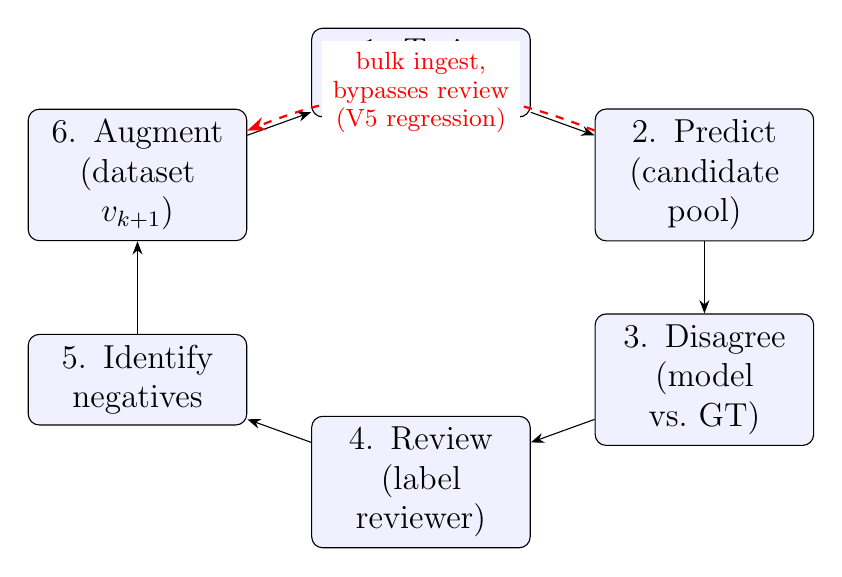
\begin{tikzpicture}[>=Stealth, font=\small,
      n/.style={draw, rounded corners, align=center, minimum height=9mm, text width=25mm, fill=blue!6}]
      \node[n] (train) at (0,2.6)    {1. Train\\model $v_k$};
      \node[n] (pred)  at (3.6,1.3)  {2. Predict\\(candidate pool)};
      \node[n] (dis)   at (3.6,-1.3) {3. Disagree\\(model vs.\ GT)};
      \node[n] (rev)   at (0,-2.6)   {4. Review\\(label reviewer)};
      \node[n] (neg)   at (-3.6,-1.3){5. Identify\\negatives};
      \node[n] (aug)   at (-3.6,1.3) {6. Augment\\(dataset $v_{k+1}$)};
      \draw[->] (train)--(pred); \draw[->] (pred)--(dis); \draw[->] (dis)--(rev);
      \draw[->] (rev)--(neg);   \draw[->] (neg)--(aug);  \draw[->] (aug)--(train);
      \draw[->, red, dashed, thick] (pred) to[bend right=22]
            node[midway, fill=white, font=\scriptsize, text=red, align=center]
            {bulk ingest,\\bypasses review\\(V5 regression)} (aug);
    \end{tikzpicture}
    \caption{The HITL co-evolution loop. The disciplined path (blue) routes every candidate batch through Disagree$\rightarrow$Review before it is augmented into the next dataset. The V5 regression (\S\ref{sec:ir_evolution}) took the red shortcut: a large positive batch was ingested directly, bypassing review, so unlabelled drones entered training and were scored as false positives.}
    \label{fig:hitl_loop}
\end{figure}

The key observation is that a well-performing model's disagreement with GT is informative regardless of which side is right. A model FP is either a real error (needs a hard negative) or an annotation error (correct the GT); a model FN is either a real miss (hard positive) or a spurious GT box (remove the GT). In either case the disagreement is actionable rather than ambiguous. The empirical record of the loop is the precision/recall trace in \S\ref{sec:ir_evolution}.

\section{Case Study: IR Detector Evolution V2 $\to$ Final $\to$ v3b}
\label{sec:ir_evolution}

The IR detector was developed across five numbered revisions (V2 through V6) plus a \texttt{Final} retrain and a \texttt{v3b} corrective fine-tune. Earlier discussions of this work reported a per-version best-epoch mAP50 number from each model's training run, which is not directly comparable across versions because the val split changed with the dataset. To produce comparable numbers, every version was re-evaluated on the same fixed \texttt{IR\_dset\_final} test split at \texttt{imgsz=640} (\textsc{Ledger}~\S4.1; script: \texttt{eval/eval\_ir\_versions.py}).

\begin{table}[htbp]
    \centering
    \caption{IR detector versions evaluated on the fixed \texttt{IR\_dset\_final} test split @ \texttt{imgsz=640}. Comparable across versions; supersedes the per-version best-epoch mAP narrative. \texttt{v3b} is the production weight; all earlier versions, including \texttt{Final}, are superseded. Source: \textsc{Ledger}~\S4.1.}
    \label{tab:ir_evolution}
    \begin{tabular}{lcccccc}
        \toprule
        Version & mAP50 & mAP50-95 & $P$ & $R$ & F1 & Status \\
        \midrule
        V2     & 0.458 & 0.219 & 0.661 & 0.406 & 0.503 & superseded \\
        V3     & 0.571 & 0.242 & 0.648 & 0.579 & 0.611 & superseded \\
        V4     & 0.722 & 0.393 & 0.895 & 0.669 & 0.765 & superseded \\
        V5     & 0.694 & 0.446 & 0.768 & 0.709 & 0.737 & superseded (regression) \\
        V6     & 0.956 & 0.571 & 0.921 & 0.941 & 0.931 & superseded \\
        Final  & \textbf{0.977} & \textbf{0.602} & 0.955 & \textbf{0.980} & 0.967 & base for prod \\
        \textbf{v3b (production)} & 0.972 & 0.591 & \textbf{0.957} & 0.977 & \textbf{0.967} & current \\
        \bottomrule
    \end{tabular}
\end{table}

\begin{figure}[htbp]
    \centering
    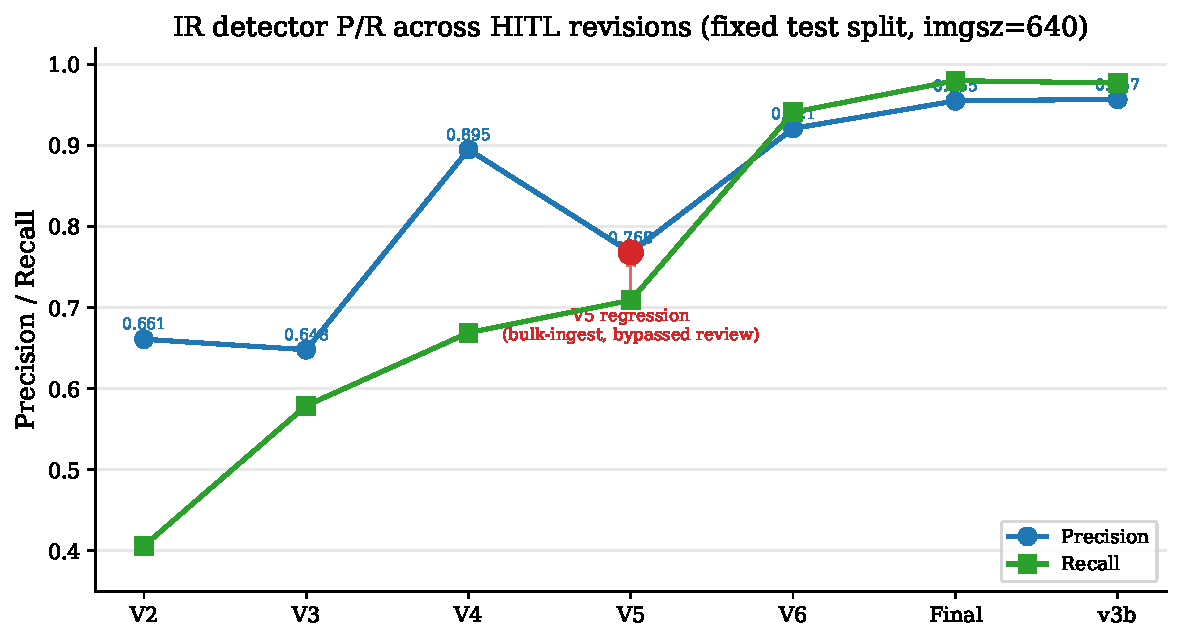
\includegraphics[width=0.85\textwidth]{fig4_ir_evolution}
    \caption{IR detector P/R trajectory across the five numbered revisions (V2--V6) plus the \texttt{Final} retrain and production \texttt{v3b}, on the fixed \texttt{IR\_dset\_final} test split. The V5 regression (precision $0.895 \to 0.768$) is recovered by V6 and the production \texttt{v3b}. Source: \textsc{Ledger}~\S4.1.}
    % [source: ledger=ir-version-progression; eval=ir_final_v3b; run=eval/ir_version_comparison.py; cache=eval/results/ir_version_comparison/ir_comparison_test_640_2026-05-16T20-04-39.csv; config=ir_final_640]
    \label{fig:ir_evolution}
\end{figure}

The trajectory can be read in four passes.

\emph{V2 $\to$ V3: a recall-driven gain off a noisier corpus.} V2 was a 300-epoch fine-tune on a broader, merged training corpus and is the weakest version on every aggregate metric (mAP50 0.458, F1 0.503), though its precision (0.661) actually exceeds V3's (0.648). The move to V3's narrower, curated subset trades a little of that precision for a large recall gain ($0.406 \to 0.579$), lifting both F1 ($0.503 \to 0.611$) and mAP50 ($0.458 \to 0.571$). The lesson is that the curated subset, not the broader merge, is the better training base --- the premise for the FP-mining and split-cleanup cycles that drive the later versions.
% [source: ledger=ir-version-progression; eval=ir_final_v3; run=eval/ir_version_comparison.py; cache=eval/results/ir_version_comparison/ir_comparison_test_640_2026-05-16T20-04-39.csv; config=ir_final_640]

\emph{V3 $\to$ V4 is a precision jump, not a recall jump.} Precision rises from 0.648 to 0.895; recall barely moves (0.579 $\to$ 0.669). The signature is that of an FP-mining cycle: V3's false positives entering V4's hard-negative set, with recall held roughly constant.
% [source: ledger=ir-version-progression; eval=ir_final_v4; run=eval/ir_version_comparison.py; cache=eval/results/ir_version_comparison/ir_comparison_test_640_2026-05-16T20-04-39.csv; config=ir_final_640]

\emph{V5 regression.} Precision drops from 0.895 to 0.768. V5 is the revision where a large batch of newly acquired positive data was injected into the training set all at once, rather than passed through the disciplined per-batch review loop of \S\ref{sec:hitl_ir}. Because the bulk batch was not reviewed first, it carried unlabelled drones, which V5 then fires on and is scored against as false positives. This is the failure mode of an undisciplined HITL loop --- bypassing the review step to ingest data in bulk --- and is the case for which V6 and \texttt{Final} are the recovery.
% [source: ledger=ir-version-progression; eval=ir_final_v5; run=eval/ir_version_comparison.py; cache=eval/results/ir_version_comparison/ir_comparison_test_640_2026-05-16T20-04-39.csv; config=ir_final_640]

\begin{figure}[htbp]
    \centering
    \fbox{\parbox{0.9\textwidth}{\centering\vspace{2cm}
        \textbf{[PLACEHOLDER --- V5 regression qualitative]} 3--4 frame panel showing scenes where V4 was correct and V5 fires on newly-ingested but unlabelled drones (scored as FP). Same scenes after corpus cleanup (V6) where the label is corrected and the model fires correctly.
    \vspace{2cm}}}
    \caption{V5 regression case study: same scenes scored as FP under V5 (label missing) and as TP under V6 (label corrected). The model state is unchanged across the V5--V6 transition in these frames; the dataset state is what moved.}
    \label{fig:v5_regression}
\end{figure}

\emph{\texttt{Final} vs v3b are indistinguishable on this split.} Both reach F1$=$0.967. \texttt{v3b} is retained as production because the 2-epoch corrective fine-tune addresses specific deployment failures (GUI regressions, particular hot-pixel scenes) not represented in this test split.
% [source: ledger=ir-version-progression; eval=ir_final_v3b; run=eval/ir_version_comparison.py; cache=eval/results/ir_version_comparison/ir_comparison_test_640_2026-05-16T20-04-39.csv; config=ir_final_640]

% ======================================================================
% CHAPTER 6 — EXPERIMENTAL RESULTS
% ======================================================================
\chapter{Experimental Results}
\label{ch:experiments}

\paragraph{Study design.}
This chapter answers the thesis's four research questions, restated and answered in full in \S\ref{sec:rq_answers}, against the datasets and scoring rules defined earlier. RQ1 (does a downstream cascade suppress the confuser false alarms the detector cannot?) is addressed by the cumulative-suppression and classifier-comparison evaluations (\S\ref{sec:cumulative}); RQ2 (what does that cost in-distribution, and is the cost surface-dependent?) by the Svanstr\"om-versus-real-video exchange (\S\ref{sec:realvideo_cascade}); RQ3 (are multi-modal results comparable across studies?) by the scoring-rule audit (\S\ref{sec:scoring_audit}); and RQ4 (does a thermal-trained detector transfer to grayscale RGB?) by the cross-modal real-video diagnostic (\S\ref{sec:grayscale}). The unit of analysis is the frame except where a per-clip or per-segment grain is stated, and the in-distribution overlaps that bound each surface are made explicit in the threats analysis (\S\ref{sec:threats}).

This chapter presents the empirical evaluation results. \S\ref{sec:cumulative} reports cumulative confuser suppression across cascade stages. \S\ref{sec:roboflow} reports the Roboflow OOD audit. \S\ref{sec:realvideo} reports the six-mode real-video diagnostic and Pareto analysis; \S\ref{sec:grayscale} examines the unexpected cross-modal transfer result. \S\ref{sec:realvideo_cascade} runs the full cascade on real video, including the classifier comparison on operational footage. \S\ref{sec:selcom} reports the SelCom CCTV evaluation. \S\ref{sec:threats} and \S\ref{sec:limits} list threats to validity and limitations. Design ablations (classifier variants, patch threshold sweep, catch-rate audit) are in Chapter~\ref{ch:architecture} \S\S\ref{sec:classifier_compare}--\ref{sec:patch_audit}.

\section{Headline: Cumulative Confuser Suppression}
\label{sec:cumulative}

The cascade is evaluated in three modes (\textsc{Ledger}~\S7): an OOD confuser-zoo mode (no GT; every detection is an FP); a Svanstr\"om paired mode (real GT; IoP@0.5 scored); and a per-classifier comparison. This is the \emph{comparison} configuration that motivated the production picks of \S\ref{sec:production_stack}, not the production stack itself: the figures below use the baseline RGB model, the IR \texttt{v3b} weights, the v2 patch verifier, \texttt{imgsz=1280}, \texttt{rgb\_conf=0.25}, \texttt{ir\_conf=0.40}. The production RGB detector (\texttt{ft4}), trust classifier (\texttt{robust8}), and per-frame verifiers (\texttt{mlp\_v5}/\texttt{mlp\_v5\_ir\_aligned}) are evaluated at the component level in \S\ref{sec:feature_selection} and \S\ref{sec:distill_verifier}; their full-cascade re-run is the registered placeholder of Figure~\ref{fig:mlp_pipeline_placeholder}.
% [source: ledger=cascade-confuser-collapse; eval=clfzoo_fnfn; run=eval/cumulative_halluc.py; cache=eval/results/_cumulative_halluc/confuser_fusion_no_fn_model_v1.1/summary.json; config=confuser_zoo_1280]

\begin{table}[htbp]
    \centering
    \caption{Confuser zoo (no GT, 2,633 OOD imgs). \texttt{fusion\_no\_fn\_v1.1} classifier, v2 patch verifier. Source: \textsc{Ledger}~\S7.}
    \label{tab:cum_confuser}
    \begin{tabular}{lrccc}
        \toprule
        Source & N & S1 fire & S2 fire & S3 fire \\
        \midrule
        AIRPLANE (roboflow) & 99 & 0.273 & 0.030 & 0.030 \\
        OTHER (svan+kaggle+roboflow) & 2,534 & 0.530 & 0.015 & 0.007 \\
        \textbf{OVERALL} & 2,633 & \textbf{0.521} & \textbf{0.016} & \textbf{0.008} \\
        \bottomrule
    \end{tabular}
\end{table}

\begin{figure}[htbp]
    \centering
    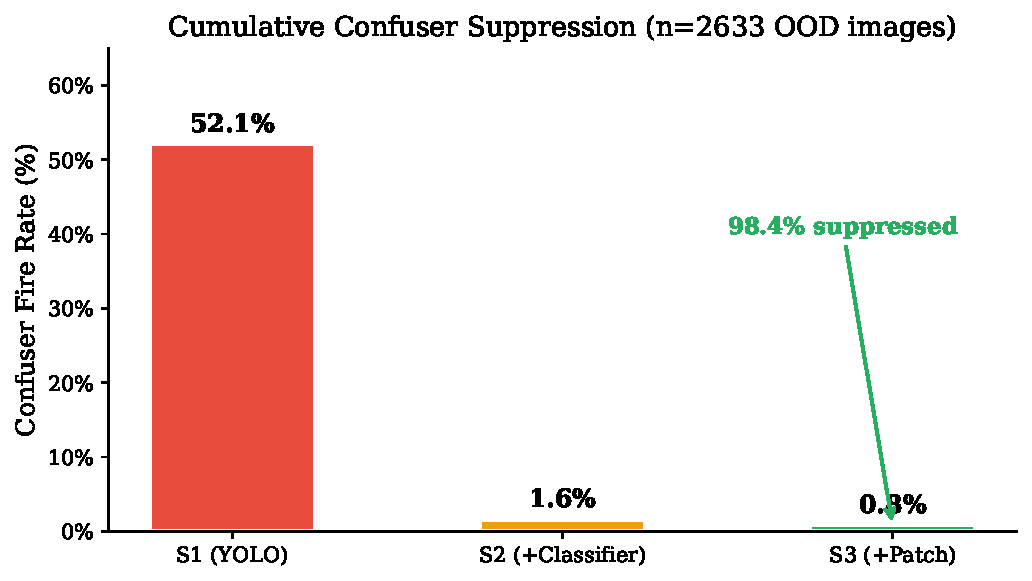
\includegraphics[width=0.75\textwidth]{fig6_1_cumulative_confuser}
    \caption{Cumulative confuser-zoo fire rate across the cascade with the open-world fallback classifier \texttt{fusion\_no\_fn\_v1.1}. The bulk of the suppression is at the classifier stage; the patch verifier roughly halves the residual. Source: \textsc{Ledger}~\S7.}
    \label{fig:cumulative_confuser}
\end{figure}

\begin{table}[htbp]
    \centering
    \caption{Svanstr\"om paired @ \texttt{imgsz=1280}, IoP@0.5, full 28,710 frames. \texttt{fusion\_no\_fn\_v1.1} classifier, v2 patch verifier. Drone class only. Source: \textsc{Ledger}~\S7.}
    \label{tab:cumulative_svanstrom}
    \begin{tabular}{lcccccc}
        \toprule
        Stage & TP & FP & FN & $P$ & $R$ & F1 \\
        \midrule
        S1 RGB alone        & 11260 & 721 & 454 & 0.940 & \textbf{0.961} & 0.950 \\
        S2 + trust classifier & 10682 & 991 & 1032 & 0.915 & 0.912 & 0.914 \\
        S3 + patch v2 (\texttt{thr=0.5}) & 9564 & 756 & 2150 & 0.927 & 0.817 & 0.868 \\
        \bottomrule
    \end{tabular}
\end{table}

\begin{figure}[htbp]
    \centering
    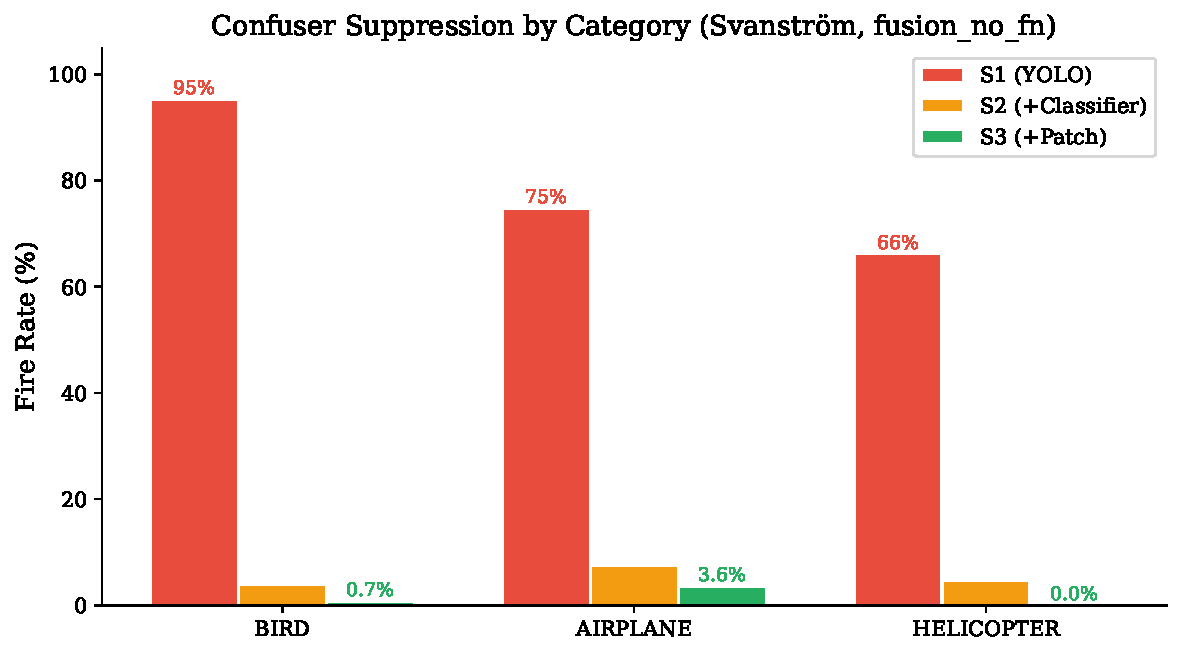
\includegraphics[width=0.85\textwidth]{fig6_2_svanstrom_by_category}
    \caption{Per-category cascade suppression on Svanstr\"om paired confuser frames. Each confuser category's S1 fire rate drops sharply at the classifier stage; the patch verifier removes the residual on helicopters (near-zero S3) and most of it on birds. Source: \textsc{Ledger}~\S7.}
    \label{fig:svanstrom_by_cat}
\end{figure}

Tables~\ref{tab:cum_confuser} and~\ref{tab:cumulative_svanstrom} are two different measurements of the same cascade with the open-world fallback classifier \texttt{fusion\_no\_fn\_v1.1}, and both numbers carry. The OOD zoo measures \emph{confuser-fire reduction}: 52.1\% $\to$ 1.6\% $\to$ 0.8\% across stages, with the classifier carrying $\sim$98\% of the cumulative suppression and the patch verifier halving the residual. The Svanstr\"om paired evaluation measures the \emph{in-distribution cost of that reduction}: drone $F1$ falls from 0.950 (S1) to 0.914 (S2) to 0.868 (S3 at \texttt{patch\_thr}$=$0.5). Recall is the part that suffers ($R: 0.961 \to 0.912 \to 0.817$); precision is roughly stable.
% [source: ledger=cascade-confuser-collapse; eval=clfzoo_fnfn; run=eval/cumulative_halluc.py; cache=eval/results/_cumulative_halluc/confuser_fusion_no_fn_model_v1.1/summary.json; config=confuser_zoo_1280]

With the sa32 comparison classifier the picture shifts. On the OOD zoo, sa32 cuts fire from 52.1\% only to 20.5\% (\S\ref{sec:classifier_compare}, Table~\ref{tab:classifiers}), an order of magnitude weaker than fnfn but still a 2.5$\times$ reduction. On Svanstr\"om paired drones, sa32 reaches Stage-3 $F1=0.895$ at the production $\mathtt{patch\_thr}=0.9$ (\S\ref{sec:patch_threshold}), roughly tied with fnfn. The fnfn numbers above are therefore the strongest OOD-suppression case (the open-world fallback's purpose) rather than the production stack's headline.
% [source: ledger=cascade-confuser-collapse; eval=svan_s3_sa32_thr08; run=(EVIDENCE_LEDGER sweep); config=svan_iop_1280_s9]

The cascade is not an unconditional improvement over S1 on in-distribution drones with the fnfn classifier. It is an exchange: in-distribution F1 for OOD safety. The \emph{operating point} of that exchange (specifically the patch-verifier threshold) is the subject of \S\ref{sec:patch_threshold}, which shows that raising \texttt{patch\_thr} from 0.5 to 0.9 recovers most of the S3 recall loss (back to $R=0.869$, $F1=0.895$) at a small confuser-FP cost. The production cascade on Svanstr\"om-style inputs ships at \texttt{patch\_thr}$=$0.9; the OOD zoo numbers above use \texttt{patch\_thr}$=$0.5 because that is the operating point that produced the run. The real-video diagnostic (\S\ref{sec:realvideo_cascade}) shows that on operationally collected footage with the sa32 comparison classifier the temporal smoother inverts this exchange entirely: the cascade gains drone $F1$ over the Stage-1 RGB number while still cutting confuser FPR threefold. The exchange between in-distribution F1 and OOD safety is therefore a property of the classifier and evaluation surface, not of the cascade architecture itself.
% [source: ledger=cascade-segment-recovers; eval=svan_s3_sa32_thr08,pipe_vid_baseline_seg; run=(EVIDENCE_LEDGER sweep); config=svan_iop_1280_s9]

\begin{figure}[htbp]
    \centering
    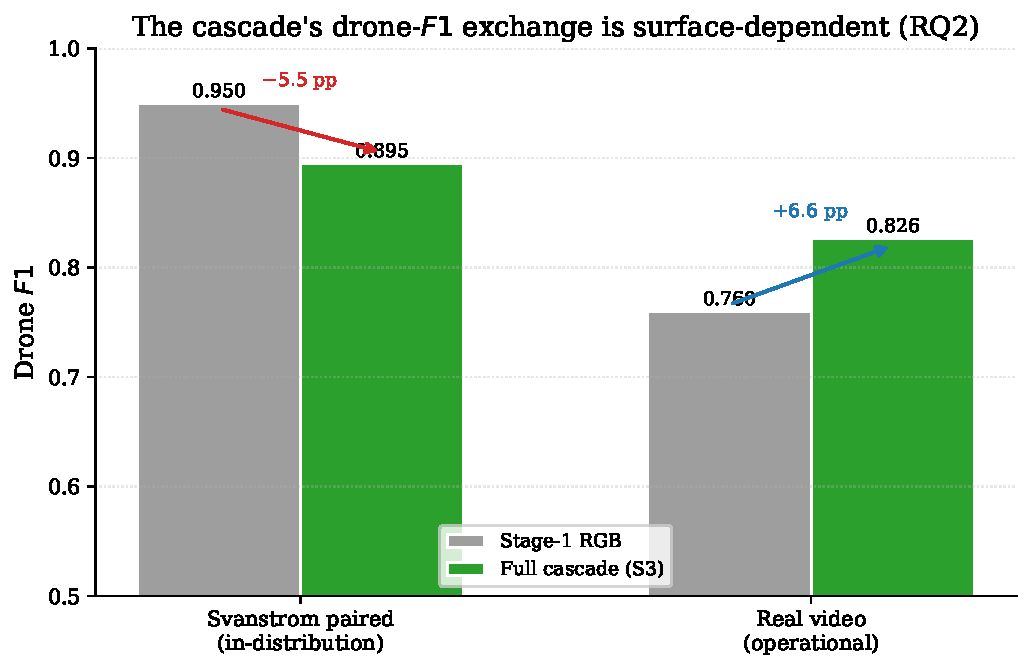
\includegraphics[width=0.72\textwidth]{fig8_surface_exchange}
    \caption{The cascade's drone-$F1$ exchange is surface-dependent (RQ2). On in-distribution Svanstr\"om-paired data the full cascade \emph{costs} $5.5$~pp drone $F1$ ($0.950\to0.895$, sa32 at \texttt{patch\_thr}=0.9); on operational real video it \emph{gains} $6.6$~pp ($0.760\to0.826$) as temporal smoothing recovers per-frame misses. Same architecture, opposite sign. Source: \textsc{Ledger}~\S7, \S9.5.}
    % [source: ledger=cascade-segment-recovers; eval=rgb_svan_baseline,svan_s3_sa32_thr08,pipe_vid_baseline_seg; run=eval/diagnose_failures.py; config=svan_iop_1280]
    \label{fig:surface_exchange}
\end{figure}
% [source: ledger=trust-classifier-conditional; eval=svan_s3_sa32_thr08; run=(EVIDENCE_LEDGER sweep); config=svan_iop_1280_s9]

\section{OOD: Roboflow Audit}
\label{sec:roboflow}

The Roboflow OOD audit (\textsc{Ledger}~\S8) evaluates the RGB and IR detectors on nine community datasets at \texttt{imgsz=640}, scored against the datasets' own labels (where present) or counted as pure-FP frames (where no GT exists). The patch verifier is run as a per-frame filter in this evaluation; the trust classifier is not run. The audit therefore measures detector + patch verifier OOD behaviour in isolation. Full analysis: \texttt{docs/analysis/2026-05-16\_roboflow\_ood\_eval.md}.

\subsection{Aggregated RGB Drone Performance}

\begin{table}[htbp]
    \centering
    \caption{RGB drone detection across the Roboflow \texttt{rgb\_drone} splits. Source: \textsc{Ledger}~\S8.1.}
    \label{tab:ood_rgb_drone}
    \begin{tabular}{llccc}
        \toprule
        Model & Stage & $P$ & $R$ & F1 \\
        \midrule
        baseline      & raw           & 0.912 & 0.746 & 0.820 \\
        baseline      & + patch v2    & 0.927 & 0.690 & 0.792 \\
        \texttt{retrained\_v2}  & raw           & 0.924 & 0.726 & 0.813 \\
        \texttt{retrained\_v2}  & + patch v2    & 0.929 & 0.686 & 0.790 \\
        \bottomrule
    \end{tabular}
\end{table}

Two findings. First, the baseline RGB detector wins on OOD drone recall ($R=0.746$ vs $R=0.726$ for \texttt{retrained\_v2}), confirming that \texttt{retrained\_v2}'s Svanstr\"om collapse is not a generalisable recall defect (OOD recall is within $2$~pp of baseline); the collapse is specific to the small, distant drones that the \texttt{imgsz} sweep of \S\ref{sec:resolution_arch} shows are resolution-bound. Second, the patch verifier costs net F1 on \emph{every} drone setting at \texttt{imgsz=640} ($-2.3$ to $-2.8$~pp). The verifier is severely distribution-bound: it was trained on Svanstr\"om-scale confuser crops, and on the OOD Roboflow imagery its bird/airplane/helicopter discrimination capacity does not transfer at the same rate that its drone-veto rate does.
% [source: ledger=selcom-ood-confuser-damage; eval=rob_rgb_baseline; run=eval/run_roboflow_eval.py; config=roboflow_rgb_drone_640]

\subsection{Aggregated RGB Confuser FP Suppression}

\begin{table}[htbp]
    \centering
    \caption{Patch verifier RGB confuser FP suppression on Roboflow OOD splits. Source: \textsc{Ledger}~\S8.2.}
    \label{tab:ood_rgb_confuser}
    \begin{tabular}{lcccc}
        \toprule
        Confuser & baseline supp\% & \texttt{retrained\_v2} supp\% & Total cuts (best) & Notes \\
        \midrule
        airplane   &  3.1\% &  1.9\% &  $\leq$32 & verifier ineffective on OOD airplanes \\
        bird       & 50.5\% & 51.8\% & 52 & verifier transfers well to OOD birds \\
        helicopter & 36.1\% &  8.1\% & 165 & baseline-favored \\
        \bottomrule
    \end{tabular}
\end{table}

The Svanstr\"om-vs-Roboflow gap is dramatic: 52\% airplane suppression on Svanstr\"om vs 3.1\% on Roboflow. The likely explanation is dataset-induced: Svanstr\"om airplanes are predominantly small-and-distant, matching the verifier's training distribution, whereas Roboflow airplanes are typically large-and-close (often filling the frame), a regime underrepresented in the verifier's training set. Bird suppression transfers (50--52\%) because the small-bird regime is consistent across the two sources. This is what the cascade chapter calls the verifier's ``OOD ceiling''.
% [source: ledger=patch-verifier-distribution-bound; eval=rob_rgb_baseline; run=eval/run_roboflow_eval.py; config=roboflow_rgb_drone_640]

\subsection{IR Drone and Confuser Performance}

\begin{table}[htbp]
    \centering
    \caption{IR detector on Roboflow OOD drone splits. Source: \textsc{Ledger}~\S8.3.}
    \label{tab:ood_ir}
    \begin{tabular}{llccc}
        \toprule
        Dataset & Stage & $P$ & $R$ & F1 \\
        \midrule
        \texttt{ir\_drone\_night} & raw & 0.494 & \textbf{0.264} & 0.344 \\
        \texttt{ir\_drone\_night} & + patch v2 & 0.474 & 0.210 & 0.291 \\
        \texttt{ir\_mixed\_cbam}  & raw & 0.821 & 0.519 & 0.636 \\
        \texttt{ir\_mixed\_cbam}  & + patch v2 & 0.874 & 0.491 & 0.628 \\
        \bottomrule
    \end{tabular}
\end{table}

The IR detector has a hidden OOD ceiling. On in-distribution thermal data (Anti-UAV, Svanstr\"om IR) it reaches $R \geq 0.945$; on \texttt{ir\_mixed\_cbam} recall drops to $R=0.519$ and on \texttt{ir\_drone\_night} to $R=0.264$. The \texttt{ir\_drone\_night} number is partly an artefact of the dataset (heavy synthetic noise / blur / contrast augmentations applied per-image), but the \texttt{ir\_mixed\_cbam} number is on cleaner data and is a real generalisation gap. The IR detector belongs in the thesis limitations chapter for this reason (\S\ref{sec:limits}).
% [source: ledger=ir-ood-recall-ceiling; eval=ir_ood_cbam_raw; run=(EVIDENCE_LEDGER sweep); config=roboflow_ir_drone_640]

\section{Real-Video Six-Mode Diagnostic}
\label{sec:realvideo}

Beyond the Roboflow OOD audit, a separate real-video diagnostic was conducted on 19 curated YouTube clips: 9 drone-positive videos (1{,}234 ground-truth drone frames, several with birds in the same frame), 10 confuser-only videos (1{,}250 frames, no drones present), all visually inspected. Six detector modes were compared on the same videos at \texttt{conf=0.25}, IoP@0.5: the three RGB detector variants (baseline, the aggressively confuser-augmented \texttt{retrained\_v2}, and the SelCom CCTV fine-tune \texttt{Yolo26n\_selcom\_mixed\_ft2\_1280} at its native \texttt{imgsz=1280}); the same SelCom fine-tune evaluated at \texttt{imgsz=640} (\texttt{selcom\_640}) as a resolution ablation; and the IR detector \texttt{v3b} fed either grayscale-converted RGB or raw RGB. Source: \textsc{Ledger}~\S9.4 (re-run 2026-05-18 with corrected scoring; supersedes \S\S9.1--9.3 for the metrics tabulated here).
% [source: ledger=ir-grayscale-fallback; eval=vid_drone_ir_gray; run=eval/eval_video_tests.py; config=video_drone_iop]

\begin{table}[htbp]
    \centering
    \caption{Real-video six-stack diagnostic. Drone columns: aggregate $P$, $R$, $F1$ across 9 drone-positive videos (1{,}234 GT drone instances). FPPI columns: false positives per image on confuser-only videos. Cells in \textbf{bold} mark the best (or tied-best) value per column for the trade-off being read. Source: \textsc{Ledger}~\S9.4 (re-run 2026-05-18 with corrected scoring; supersedes \S\S9.1--9.3 for these metrics).}
    \label{tab:realvideo_master}
    \begin{tabular}{lccccccc}
        \toprule
        & \multicolumn{3}{c}{Drone (9 videos)} & \multicolumn{4}{c}{Confuser FPPI (10 videos)} \\
        \cmidrule(lr){2-4} \cmidrule(lr){5-8}
        Mode & $P$ & $R$ & $F1$ & All & Bird & Airplane & Helicopter \\
        \midrule
        RGB baseline           & 0.771 & 0.749 & \textbf{0.760} & 0.512 & 0.960 & 0.451 & 0.278 \\
        RGB \texttt{retrained\_v2} & \textbf{0.909} & 0.453 & 0.605 & 0.196 & 0.139 & 0.385 & 0.133 \\
        RGB \texttt{selcom\_1280}  & 0.649 & \textbf{0.812} & 0.721 & 0.709 & 1.528 & 0.493 & 0.333 \\
        RGB \texttt{selcom\_640}\,$^{\dagger}$  & 0.807 & 0.666 & 0.730 & 0.260 & 0.313 & 0.359 & 0.179 \\
        \textbf{IR on grayscale-RGB} & 0.743 & 0.557 & 0.636 & \textbf{0.158} & \textbf{0.142} & \textbf{0.283} & \textbf{0.103} \\
        IR on raw RGB          & 0.647 & 0.191 & 0.295 & 0.150 & 0.261 & 0.158 & 0.079 \\
        \bottomrule
    \end{tabular}
    \\[2pt]
    \footnotesize $^{\dagger}$\,\texttt{selcom\_640} runs the same \texttt{Yolo26n\_selcom\_mixed\_ft2\_1280} weights at \texttt{imgsz=640}; it isolates the contribution of input resolution from the fine-tune itself.
\end{table}

\begin{figure}[htbp]
    \centering
    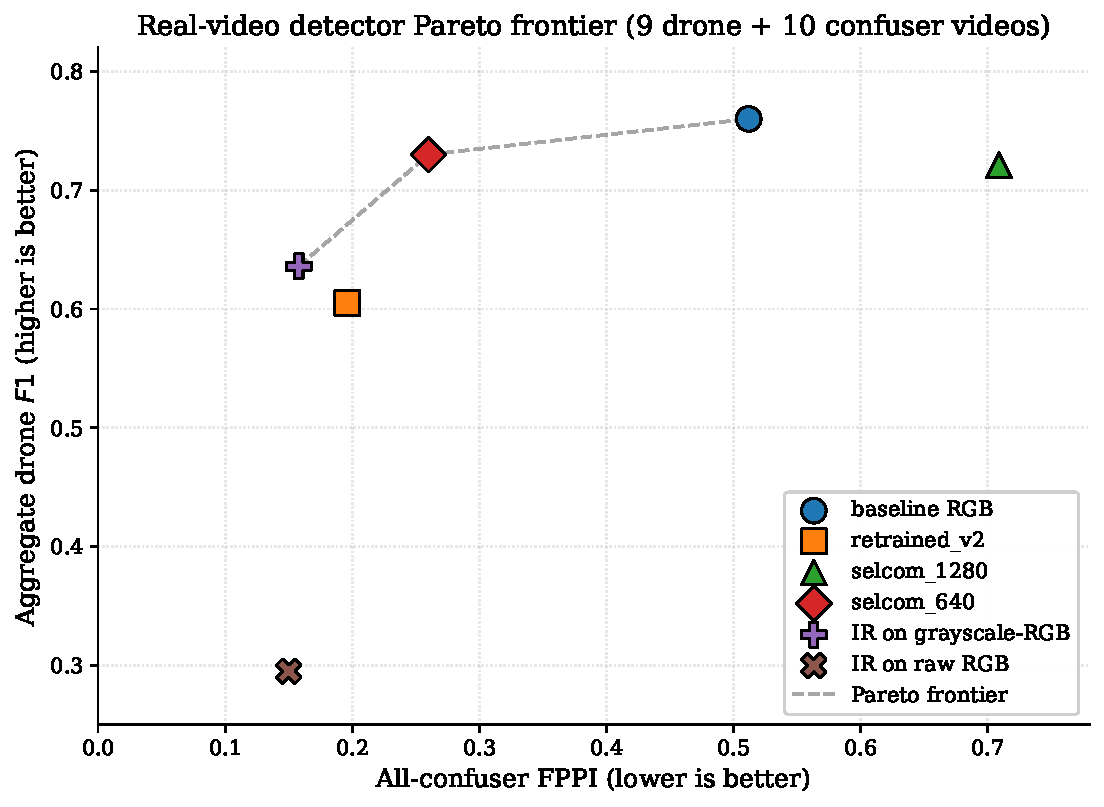
\includegraphics[width=0.85\textwidth]{fig5_realvideo_pareto}
    \caption{Six detector modes on the joint (drone $F1$, all-confuser FPPI) axis. The Pareto frontier has three points: IR on grayscale-RGB, \texttt{selcom\_640}, and RGB baseline. \texttt{retrained\_v2} and \texttt{selcom\_1280} are Pareto-dominated. Source: \textsc{Ledger}~\S9.4.}
    \label{fig:realvideo_pareto}
\end{figure}

Table~\ref{tab:realvideo_master} characterises all six detector modes on the same clips under one scoring rule, so the trade-offs below can be read directly off it.

\paragraph{Three-mode recall--precision continuum among the RGB detectors.}
The three RGB variants occupy three distinct points: \texttt{retrained\_v2} at high precision / low recall ($P=0.909, R=0.453$), \texttt{selcom\_1280} at high recall / lower precision ($P=0.649, R=0.812$), and the baseline in between. The training corpus determines the position. \texttt{retrained\_v2}'s aggressive confuser-augmented training has effectively taught it to suppress small-sky targets, which inflates drone precision (it does not fire on birds) but collapses drone recall in bird-cluttered scenes. \texttt{selcom\_1280}'s CCTV-drone fine-tune has lowered its detection floor on small sky objects, which lifts drone recall but also inflates bird FPPI to 1.528 (above one false positive per confuser frame on average). The \texttt{selcom\_640} row (same weights, lower inference resolution) shows that roughly half of selcom's drone-recall win and almost all of its confuser-FPPI penalty come from running the fine-tuned weights at \texttt{imgsz=1280}; at \texttt{imgsz=640} the fine-tune yields a cleaner trade ($F1=0.730$ drone, FPPI=0.260). Production deployment should pick by scene-distribution expectation rather than treat any single RGB variant as dominant.
% [source: ledger=no-pareto-dominance-video; eval=vid_drone_baseline; run=eval/eval_video_tests.py; config=video_drone_iop]

\paragraph{The Pareto frontier has three points, only one of which is RGB-baseline.}
Three modes are Pareto-optimal on the joint (drone $F1$, all-confuser FPPI) axis: the IR detector on grayscale-RGB (0.636, 0.158), \texttt{selcom\_640} (0.730, 0.260), and the RGB baseline (0.760, 0.512). The IR-on-grayscale point trades $-12.4$~pp drone $F1$ versus the baseline for a $3.2\times$ reduction in confuser FPPI ($0.512 \to 0.158$), and on the bird-FPPI column specifically it is $6.8\times$ better ($0.960 \to 0.142$). \texttt{selcom\_640} sits between the two and is in fact the cleanest single-detector point at FPPI~$\leq$~0.3. \texttt{retrained\_v2} and \texttt{selcom\_1280} are both Pareto-dominated, \texttt{retrained\_v2} by IR-on-grayscale (higher F1, lower FPPI), \texttt{selcom\_1280} by the baseline (higher F1, lower FPPI). That the IR detector is on this frontier at all is unexpected, since the model has never seen visible-light imagery in training; the transfer is examined in detail in \S\ref{sec:grayscale}.
% [source: ledger=no-pareto-dominance-video; eval=vid_drone_ir_gray; run=eval/eval_video_tests.py; config=video_drone_iop]

\paragraph{The hardest single video, \texttt{flock\_of\_seagulls\_attack\_drone\_beach} (239 frames, 187 drone GT).}

\begin{table}[htbp]
    \centering
    \caption{Per-mode drone detection on a single representative bird-cluttered video. The IR detector on grayscale-RGB matches the RGB baseline within a third of a percentage point of $F1$, on a video it has no business detecting since it was trained on thermal data only, while every other variant trails by 5--58~pp. Source: \textsc{Ledger}~\S9.4.}
    \label{tab:realvideo_seagull}
    \begin{tabular}{lccc}
        \toprule
        Mode & $P$ & $R$ & $F1$ \\
        \midrule
        \textbf{RGB baseline}           & 0.940 & 0.759 & \textbf{0.840} \\
        RGB \texttt{retrained\_v2} & \textbf{1.000} & 0.439 & 0.610 \\
        RGB \texttt{selcom\_1280}  & 0.578 & \textbf{0.877} & 0.696 \\
        RGB \texttt{selcom\_640}   & 0.977 & 0.668 & 0.794 \\
        \textbf{IR on grayscale-RGB} & 0.917 & 0.770 & \textbf{0.837} \\
        IR on raw RGB          & 0.966 & 0.150 & 0.259 \\
        \bottomrule
    \end{tabular}
\end{table}

\noindent The IR detector on grayscale-RGB ties the RGB baseline on the hardest bird-cluttered drone clip in the diagnostic ($F1 = 0.837$ vs $0.840$, a difference of $0.003$). It is the strongest result the IR-on-grayscale mode produces on a single clip, and the only setting in which a thermal-trained model is competitive with the best dedicated RGB detector on visible-light video. \texttt{selcom\_640} comes in third at $F1=0.794$; the production CCTV weights at \texttt{imgsz=1280} (\texttt{selcom\_1280}) trail at $F1=0.696$ because their lowered detection floor produces 120 bird-induced false positives on this clip alone.
% [source: ledger=ir-grayscale-fallback; eval=vid_drone_ir_gray; run=eval/eval_video_tests.py; config=video_drone_iop]

\section{IR Model on Grayscale RGB: An Unexpected Cross-Modal Result}
\label{sec:grayscale}

The IR detector was trained exclusively on thermal infrared data. Its training set contained no visible-light imagery. The grayscale-RGB operating mode in the deployed GUI exists because thermal cameras are expensive and not always available; when only an RGB stream is on hand, the system converts it to single-channel grayscale and feeds it to the IR model as a \emph{fallback}. This was a deployment necessity, not a designed capability. The empirical question, and the subject of this section, is whether the fallback works.

\subsection{Setup}

The grayscale mode was evaluated on the real-video diagnostic set introduced in \S\ref{sec:realvideo}: 9 drone-positive YouTube clips (1{,}234 GT drone instances) and 10 confuser-only clips (1{,}250 frames). Each clip was run through the IR detector twice, once on \texttt{cvtColor(BGR2GRAY)} of the RGB stream (replicated to 3 channels), and once on the raw 3-channel RGB stream as a control, at \texttt{imgsz=640}, \texttt{conf=0.25}, IoP@0.5. Both modes are out-of-distribution for the IR detector; the comparison isolates whether the grayscale conversion is the load-bearing step.
% [source: ledger=ir-grayscale-fallback; eval=vid_drone_ir_gray; run=eval/eval_video_tests.py; config=video_drone_iop]

\subsection{Result}

\begin{table}[htbp]
    \centering
    \caption{IR detector on grayscale-converted RGB vs raw RGB video. Both modes are zero-shot, the IR detector was trained exclusively on thermal data. Grayscale conversion more than doubles aggregate drone F1 and nearly halves bird-confuser FPPI. Source: \textsc{Ledger}~\S9.4.}
    \label{tab:ir_grayscale}
    \begin{tabular}{lccc}
        \toprule
        Mode & Drone $F1$ & Drone $R$ & Confuser bird FPPI \\
        \midrule
        IR on raw RGB             & 0.295 & 0.191 & 0.261 \\
        \textbf{IR on grayscale-RGB} & \textbf{0.636} & \textbf{0.557} & \textbf{0.142} \\
        \bottomrule
    \end{tabular}
\end{table}

Two facts. The grayscale variant more than doubles drone F1 ($0.295 \to 0.636$). And the same grayscale variant nearly halves bird-confuser FPPI ($0.261 \to 0.142$). The single change responsible for both is the conversion of three RGB colour channels to one intensity channel. The IR detector has no idea it is looking at sunlight rather than thermal emission; what it has is the intensity-gradient structure it learned from thermal training, and that structure survives the modality swap when colour is removed.
% [source: ledger=ir-grayscale-fallback; eval=vid_drone_ir_gray; run=eval/eval_video_tests.py; config=video_drone_iop]

A separate per-video result anchors the magnitude. On the single bird-cluttered drone video \texttt{flock\_of\_seagulls\_attack\_drone\_beach}, the IR detector on grayscale-RGB reaches $P=0.917$, $R=0.770$, $F1=0.837$. That is numerically on par with the strongest RGB detector on the same clip (the RGB baseline at $F1=0.840$, a $0.003$ gap that a single 187-GT clip cannot meaningfully resolve) and well above the other three RGB variants in the diagnostic (\S\ref{sec:realvideo}, Table~\ref{tab:realvideo_seagull}). The fallback intended as a degradation mode for missing thermal hardware reaches, on this single hardest bird-vs-drone clip (187 GT), drone-detection $F1$ statistically indistinguishable from the best visible-light detector in the project ($0.837$ vs $0.840$), despite having seen no visible-light imagery in training; one 187-GT clip cannot establish a general parity claim, and the aggregate (Table~\ref{tab:realvideo_master}) keeps IR-on-grayscale $12.4$~pp below the baseline.
% [source: ledger=ir-grayscale-fallback; eval=vid_drone_ir_gray; run=eval/eval_video_tests.py; config=video_drone_iop]

\begin{figure}[htbp]
    \centering
    \fbox{\parbox{0.9\textwidth}{\centering\vspace{2.2cm}
        \textbf{[PLACEHOLDER: Fig 6.7 --- Grayscale transfer qualitative panel]} Three rows, each a frame from \texttt{flock\_of\_seagulls\_attack\_drone\_beach}: (top) original RGB with baseline-RGB detections; (middle) the same frame converted to grayscale-RGB, with IR-detector-on-grayscale detections; (bottom) the raw 3-channel RGB fed to the IR detector, with its (collapsed) detections. The middle row should land the drone box where the bottom row does not.
    \vspace{2.2cm}}}
    \caption{Cross-modal transfer, illustrated. The IR detector, trained zero-shot on thermal data only, locates the drone on grayscale-converted RGB frames where its raw-RGB counterpart collapses. The transfer is preserved by the single-channel intensity input; the colour information that distinguishes thermal from visible is the part that breaks it.}
    \label{fig:grayscale_qualitative}
\end{figure}

\subsection{Why the result was unexpected}

Three reasons converge. First, the IR detector was trained with thermal-specific cues that grayscale-RGB does not preserve: motor hot-spots, battery thermal signatures, electronic-speed-controller heat blobs. A naive prior would predict that removing those cues collapses drone detection. The data shows it does not collapse.

Second, the IR-detector training corpus contains negative examples of birds, airplanes, and helicopters \emph{in the thermal modality} (\S\ref{sec:hitl_ir}). It has never been shown a visible-light bird. Yet on the confuser-only video set, the IR detector on grayscale-RGB hallucinates on bird frames at FPPI $0.142$, a $6.8\times$ reduction versus the RGB baseline ($0.960$), and essentially equal to \texttt{retrained\_v2}'s $0.139$ (a $0.003$ gap the per-clip sampling error of \S\ref{sec:threats} cannot resolve; the latter was trained with explicit visible-light bird negatives). The IR model's thermal-domain confuser training appears to transfer to the grayscale modality, landing within sampling error of a detector that was explicitly hard-negative-mined for visible-light birds.
% [source: ledger=ir-grayscale-fallback; eval=vid_conf_ir_gray; run=eval/eval_video_tests.py; config=video_confuser]

Third, the design rationale for retaining grayscale fallback in the GUI was conservative: provide \emph{some} drone-detection capability when thermal hardware is offline, with the expectation that an RGB detector would still be the primary stream. The data inverts that assumption on bird-cluttered scenes. The fallback is not a stopgap; in bird-cluttered scenes specifically it is competitive with or better than every RGB variant on the joint $F1$--FPPI trade.

\subsection{Mechanism, with the right caveats}

The likely mechanism is shared low-level statistics. Thermal IR and grayscale RGB are both single-channel intensity images. Both render small drones as a dark-on-bright (or bright-on-dark) silhouette against sky. A YOLO detector trained on thermal drone-silhouette intensity-gradient features evidently retains those features when applied to a visible-light single-channel input, since the gradient structure of a sky-background silhouette is similar across the two modalities.

The transfer is not perfect, and its limits are visible in the data. The IR detector on grayscale-RGB underperforms the RGB baseline on clean drone takeoff videos by 28--41~pp F1 on a per-clip basis (e.g.\ \texttt{drone\_takeoff\_short} 0.540 vs 0.906, \texttt{drone\_takeoff\_short\_trees\_background\_dji} 0.480 vs 0.887; Table~\ref{tab:realvideo_master} aggregates and \textsc{Ledger}~\S9.4 per-video JSONs). On bird-cluttered drone scenes it is competitive with or beats the RGB baseline. The pattern is consistent with a detector that has learned silhouette-recognition strongly and texture-recognition weakly: clean drone close-ups in good lighting expose texture-rich drone bodies that the RGB detectors capture better; small drones against cluttered sky are silhouette-dominated and the IR detector's bird-vs-drone-silhouette discrimination dominates.
% [source: ledger=ir-grayscale-fallback; eval=vid_drone_ir_gray; run=eval/eval_video_tests.py; config=video_drone_iop]

\subsection{Relation to prior work}

To our knowledge, no published study quantifies the specific transfer measured here: a thermal-only-trained drone detector evaluated zero-shot on grayscale-converted visible-light video, on drone-positive data with ground-truth boxes. The closest adjacent work is on modality hallucination (training one modality to inform another)~\cite{hoffman2016modalityhallucination}, on RGB-to-thermal style translation~\cite{berg2018rgb2thermal,kniaz2018thermalgan}, and on multimodal pretraining (where the network is \emph{trained} to be multimodal). None of these match the setup here, in which no cross-modal information is provided at training time and the transfer emerges from shared low-level structure.

The finding is therefore presented as a measured emergent property of training on a single intensity-channel modality, not as a designed capability. Its practical implication, that an IR detector trained from a difficult-to-acquire thermal dataset becomes useful on the modality (grayscale RGB) the system actually has at hand, is what makes this result load-bearing rather than incidental.

\subsection{From Cross-Modal Transfer to a Deployable Thermal Verifier}
\label{sec:grayscale_verifier}

The same cross-modal equivalence that the feature-space analysis established (\S\ref{sec:ir_xmodal_verifier}) has a deployment payoff that reverses an earlier conclusion of this project. The IR detector's grayscale mode is, for confuser frames, its \emph{hallucination} mode: \texttt{v3b} fires on grayscale confusers about $20\times$ more often than on thermal ones ($37.2\%$/image vs $1.8\%$). That liability is precisely what makes grayscale a rich, abundant source of confuser detections to harvest --- the opposite of the scarce labelled thermal confusers that had blocked a thermal verifier.
% [source: ledger=ir-grayscale-is-hallucination-mode; eval=none (MRI harvest); run=mri/modality_probe.py; cache=mri/results/ir_v3b_report; config=ir_v3b]

The production checkpoint \texttt{mlp\_v5\_ir\_aligned} combines thermal drone detections (for recall safety) with grayscale-harvested confusers, per-modality z-aligned into a single $517$-D verifier that loads in the production \texttt{MLPVerifier}. It is \emph{one network with two per-modality input scalers}: a thermal scaler (\texttt{mlp\_aligned.pt}) and a grayscale scaler (\texttt{mlp\_aligned\_gray.pt}) share the same weights and differ only in the $(\mu,\sigma)$ standardisation folded into the input, so a single trained verifier serves both the thermal-deploy and grayscale-fallback paths. CBAM --- a novel thermal aerial-confuser set --- is held out of training, so Table~\ref{tab:ir_aligned} measures generalisation, not memorisation.

\begin{table}[htbp]
    \centering
    \caption{Thermal-deploy verifier (\texttt{mlp\_v5\_ir\_aligned}, scaler \texttt{mlp\_aligned.pt}, \texttt{conf}$=$0.40, \texttt{thr}$=$0.05) vs the bare IR detector; FP in parentheses. CBAM is held out of training. The verifier cuts held-out novel-confuser false positives by $69\%$ ($48\to15$, $+0.147$~$F1$) while preserving thermal drone recall on the in-distribution surfaces ($\Delta R$ at most $-0.007$); the held-out CBAM row itself trades $-0.050$ drone recall, the residual cost on a novel confuser domain. The MobileNetV3 patch verifier on the same held-out CBAM cuts only $7$ FP. Source: \textsc{Ledger}~ir-grayscale-harvest-solves-thermal-verifier, ir-recall-fixed-by-drone-diversity.}
    \label{tab:ir_aligned}
    \begin{tabular}{lrccc}
        \toprule
        Surface & $n$ & bare IR (\texttt{v3b}) $P/R/F1$ (FP) & + aligned MLP $P/R/F1$ (FP) & $\Delta R / \Delta F1$ \\
        \midrule
        \textbf{CBAM (held out)}  & 180  & $0.547/0.967/0.699$ (48) & $\mathbf{0.786/0.917/0.846}$ (\textbf{15}) & $-0.050 / \mathbf{+0.147}$ \\
        \texttt{ir\_dset\_final}  & 4806 & $0.965/0.965/0.965$ (109) & $0.965/0.958/0.962$ (108) & $-0.007 / -0.003$ \\
        \texttt{ir\_video} test   & 831  & $0.909/0.977/0.942$ (80) & $0.909/0.977/0.942$ (80) & $0.000 / 0.000$ \\
        Anti-UAV test             & 4269 & $0.983/0.942/0.962$ (68) & $0.983/0.942/0.962$ (68) & $0.000 / 0.000$ \\
        \midrule
        \emph{patch verifier on CBAM} & 180 & --- & $0.564/0.883/0.688$ (41) & (cut only 7 FP) \\
        \bottomrule
    \end{tabular}
\end{table}
% [source: ledger=ir-grayscale-harvest-solves-thermal-verifier; eval=ir_aligned_cbam_heldout; run=mri_train_aligned; config=cbam_ir_640]
% [source: ledger=ir-grayscale-harvest-solves-thermal-verifier; eval=ir_aligned_irdset_final; run=eval_run_aligned_full; config=ir_final_640]

The same network, with its grayscale scaler, also serves the grayscale-fallback path (Table~\ref{tab:ir_aligned_gray}): it cuts held-out grayscale confuser false positives by $96\%$ ($325\to12$), matching the dedicated grayscale-only filter (\texttt{mlp\_v5\_gray}, $13$ FP) at roughly \emph{half} its drone-recall cost ($\Delta R\,{-}0.053$ vs $-0.113$). So the unified verifier replaces and beats the per-mode model on the grayscale surface as well.
% [source: ledger=ir-grayscale-harvest-solves-thermal-verifier; eval=ir_aligned_gray_heldout; run=eval_run_aligned_full; config=rgb_gray_heldout_640]

\begin{table}[htbp]
    \centering
    \caption{Grayscale-deploy verifier (same net, scaler \texttt{mlp\_aligned\_gray.pt}, \texttt{conf}$=$0.25, \texttt{thr}$=$0.25); FP in parentheses. The aligned verifier matches the dedicated grayscale-only filter's confuser cut at half the recall loss. Source: \textsc{Ledger}~ir-grayscale-harvest-solves-thermal-verifier.}
    \label{tab:ir_aligned_gray}
    \begin{tabular}{lrccc}
        \toprule
        Surface & $n$ & bare ($P/R/F1$, FP) & aligned-gray ($P/R/F1$, FP) & dedicated \texttt{mlp\_v5\_gray} \\
        \midrule
        confusers (\texttt{rgb\_confusers}$\to$gray) & 1317  & --- (325 FP) & --- (\textbf{12 FP}, 96\% cut) & 13 FP (96\%), $\Delta R\,{-}0.113$ \\
        drones (\texttt{rgb\_dataset}$\to$gray)      & 17209 & $0.704/0.210/0.324$ (1307) & $0.762/0.157/0.261$ (723) & ($\Delta R\,{-}0.053$) \\
        \bottomrule
    \end{tabular}
\end{table}
% [source: ledger=ir-grayscale-harvest-solves-thermal-verifier; eval=ir_aligned_gray_heldout; run=eval_run_aligned_full; config=rgb_gray_heldout_640]

Two properties make this deployable where the earlier IR verifier was not. First, a drone-diversity re-mine (adding $\sim$30k corrective-set thermal drones) made the verifier recall-safe on held-out thermal ($\Delta R\,{-}0.007$ on \texttt{ir\_dset\_final}, $0.000$ on \texttt{ir\_video} and Anti-UAV), where an earlier IR-verifier attempt had lost $4$--$6$~pp recall; the fix indicates that loss was OOD-drone \emph{coverage}, not confuser-reliance (a YOLO-feature-only cross-validation score, $0.986$, sits essentially on the fused score $0.987$). Second, the grayscale-harvested confusers supply the confuser-rejection signal the scarce labelled thermal data alone could not. In-pool cross-validation is optimistic, so the held-out CBAM gate is the load-bearing test.
% [source: ledger=ir-recall-fixed-by-drone-diversity; eval=ir_mlp_dronediv_heldout; run=mri; config=ir_final_640]

The bound on this result is the grayscale \emph{detection} surface itself: bare \texttt{v3b} drone recall on grayscale beats raw-RGB-into-the-thermal-model (Svanstr\"om $+0.197$, \texttt{rgb\_dataset} $+0.130$, validating the cross-modal trick) but is mediocre in absolute terms ($0.33$--$0.65$ vs $0.79$--$0.98$ on thermal). Grayscale is therefore a confuser-\emph{harvesting} surface and a hardware-fallback detection surface, not a primary one. With that scope, the result reverses the project's earlier ``ship no per-frame IR verifier'' conclusion: harvesting confusers from grayscale and aligning them into thermal feature space yields a verifier that is confuser-rich and recall-safe on in-distribution thermal drones, with the held-out CBAM drone recall ($-0.050$) marking the residual cost on a novel confuser domain.
% [source: ledger=grayscale-drone-recall; eval=vid_drone_ir_gray; run=eval/eval_video_tests.py; config=video_drone_iop]

\subsection{Open questions}

Two. First, would the transfer also work in the reverse direction (RGB-trained detector on thermal)? The data here cannot answer that; only RGB-trained models on RGB and IR-trained models on grayscale-RGB were evaluated. Second, what fraction of the transfer is preserved at \texttt{imgsz=1280} vs the \texttt{imgsz=640} used here? The grayscale fallback in this thesis was evaluated at the IR detector's native \texttt{imgsz=640}; a sweep is registered as an open item.

\section{Full Cascade on Real Video}
\label{sec:realvideo_cascade}

The Stage-1 detector measurements in \S\ref{sec:realvideo} characterise how individual detectors behave on real video. The deployed system, however, is a five-stage cascade: RGB YOLO $\to$ IR YOLO on grayscale-RGB $\to$ XGBoost trust classifier $\to$ temporal 2-of-3 smoother $\to$ confuser verifier at the alert gate. Whether the Stage-1 differences survive the downstream stack, and whether the cascade earns its claimed OOD-suppression budget on real video rather than on Svanstr\"om, is what this section measures. Source: \textsc{Ledger}~\S9.5.

The cascade runs reported in this section use the MobileNetV3 \emph{patch} verifier at the alert gate (\texttt{patch\_thr}$=$0.70), the predecessor to the per-frame distilled \texttt{mlp\_v5} that is now the production verifier (\S\ref{sec:distill_verifier}). The component-level comparison (\S\ref{sec:distill_verifier}, Table~\ref{tab:distill_verifier}) shows \texttt{mlp\_v5} dominates the patch verifier on every confuser-rich surface, so the cascade numbers below are a conservative lower bound with respect to the production stack; a full-pipeline re-run with \texttt{mlp\_v5} in the alert-gate slot is a registered open item (placeholder, Figure~\ref{fig:mlp_pipeline_placeholder}).
% [source: ledger=v5-ship-per-frame; eval=v5_svan_mlp; run=eval/eval_v4_vs_patch.py; config=svan_iop_1280_s9]

\begin{figure}[htbp]
    \centering
    \fbox{\parbox{0.9\textwidth}{\centering\vspace{1.6cm}
        \textbf{[PLACEHOLDER --- pending run: full-cascade real-video re-evaluation with the per-frame \texttt{mlp\_v5} verifier]} Re-run the four-variant real-video cascade of Table~\ref{tab:cascade_segment} with \texttt{mlp\_v5} (RGB) / \texttt{mlp\_v5\_ir\_aligned} (IR) replacing the alert-gated patch verifier, as a per-frame stage. Expected: segment drone $F1$ at least matches the patch-verifier cascade (\texttt{mlp\_v5} wins or ties on every measured surface) with equal-or-lower confuser FPR, confirming the production stack on operational footage. Tracked in \textsc{Ledger}~v5-ship-per-frame.
    \vspace{1.6cm}}}
    \caption{Reminder placeholder: the production per-frame \texttt{mlp\_v5} verifier has component-level evidence (\S\ref{sec:distill_verifier}) but has not yet been run through this full real-video cascade; the numbers in this section use its patch-verifier predecessor.}
    \label{fig:mlp_pipeline_placeholder}
\end{figure}

\subsection{Setup}
The four RGB variants from \S\ref{sec:realvideo} (baseline, \texttt{retrained\_v2}, \texttt{selcom\_1280}, \texttt{selcom\_640}) were each run through the full cascade on the same 19 real-video clips (9 drone-positive, 1{,}234 GT instances; 10 confuser-only, 1{,}250 frames). Per-stage configuration: \texttt{rgb\_conf}$=$0.25, \texttt{ir\_conf}$=$0.40, \texttt{patch\_thr}$=$0.70. Classifier: \texttt{scene\_aware\_v3more\_32feat} (production pick per \textsc{Ledger}~\S1; comparison against the two alternatives \texttt{control\_v3more\_40feat} and \texttt{fusion\_no\_fn\_v1.1} appears in \S\ref{sec:realvideo_classifier} below). IR weights: \texttt{IR\_final\_cleaned}.
% [source: ledger=trust-classifier-conditional; eval=svan_s3_sa32_thr08; run=(EVIDENCE_LEDGER sweep); config=svan_iop_1280_s9]

\begin{figure}[htbp]
    \centering
    \fbox{\parbox{0.9\textwidth}{\centering\vspace{2.6cm}
        \textbf{[PLACEHOLDER: Fig 6.8 --- Per-stage cascade output on one sequence]} Same frame, four panels: (a) raw RGB detections (baseline RGB); (b) raw IR detections (\texttt{v3b} on grayscale-RGB); (c) post-classifier surviving boxes with the trust label annotated (\texttt{trust\_rgb} / \texttt{trust\_ir} / \texttt{trust\_both} / \texttt{reject\_both}); (d) post-patch-verifier final alert with $p_\text{confuser}$ on each surviving crop. Pick one Svanstr\"om sequence and one YouTube clip; show both as side-by-side rows. Turns the cascade from text + numbers into a concrete object.
    \vspace{2.6cm}}}
    \caption{The cascade made concrete on two sequences. Top row: a Svanstr\"om sequence with a small drone and a bird; bottom row: a YouTube clip from \texttt{drone\_seagull\_attack}. Each row shows what each stage removes and what survives.}
    \label{fig:cascade_per_stage}
\end{figure}

A first observation, before any cascade comparison, is that the Stage-1 RGB per-frame metrics from this pipeline run match \S\ref{sec:realvideo} exactly for every RGB variant (baseline $F1=0.760$, \texttt{retrained\_v2} $0.605$, \texttt{selcom\_1280} $0.721$, \texttt{selcom\_640} $0.730$). The two evaluation scripts produce identical detection sets at the production threshold, which is what the scoring-fix audit in \S\ref{sec:scoring_audit} was intended to establish.
% [source: ledger=cascade-perframe-misleading; eval=pipe_vid_baseline_pf; run=(EVIDENCE_LEDGER sweep); config=pipe_video_drone_iop]

\subsection{Reading per-frame metrics is misleading}

The cascade's behaviour at the per-frame grain is counter-intuitive. Inserting the trust classifier alone \emph{reduces} per-frame drone $F1$ for three of four RGB variants (Table~\ref{tab:cascade_perframe}). Baseline drops from $0.760$ to $0.586$ ($-17.4$~pp); \texttt{selcom\_1280} drops from $0.721$ to $0.537$ ($-18.4$~pp). Only \texttt{retrained\_v2} sees a small per-frame gain ($+1.0$~pp), consistent with its conservative stance: the classifier finds fewer extra false positives to introduce on a detector that already produces few.
% [source: ledger=cascade-perframe-misleading; eval=pipe_vid_baseline_pf; run=(EVIDENCE_LEDGER sweep); config=pipe_video_drone_iop]

\begin{table}[htbp]
    \centering
    \caption{Per-frame drone metrics, Stage-1 RGB versus + classifier merging. The classifier merges RGB and IR detections per its trust label; when both modalities fire on the same drone frame, the resulting joint set inflates the per-frame FP count even when both detections are correct. The per-frame grain misrepresents what production does. Source: \textsc{Ledger}~\S9.5.}
    \label{tab:cascade_perframe}
    \begin{tabular}{lcccccc}
        \toprule
        & \multicolumn{3}{c}{RGB stage only} & \multicolumn{3}{c}{+ Classifier (per-frame)} \\
        \cmidrule(lr){2-4} \cmidrule(lr){5-7}
        RGB model & $P$ & $R$ & $F1$ & $P$ & $R$ & $F1$ \\
        \midrule
        baseline           & 0.771 & 0.749 & \textbf{0.760} & 0.520 & 0.672 & 0.586 \\
        \texttt{retrained\_v2} & \textbf{0.909} & 0.453 & 0.605 & 0.632 & 0.600 & 0.615 \\
        \texttt{selcom\_1280}  & 0.649 & \textbf{0.812} & 0.721 & 0.453 & 0.660 & 0.537 \\
        \texttt{selcom\_640}   & 0.807 & 0.666 & 0.730 & 0.522 & 0.622 & 0.568 \\
        \bottomrule
    \end{tabular}
\end{table}

\begin{figure}[htbp]
    \centering
    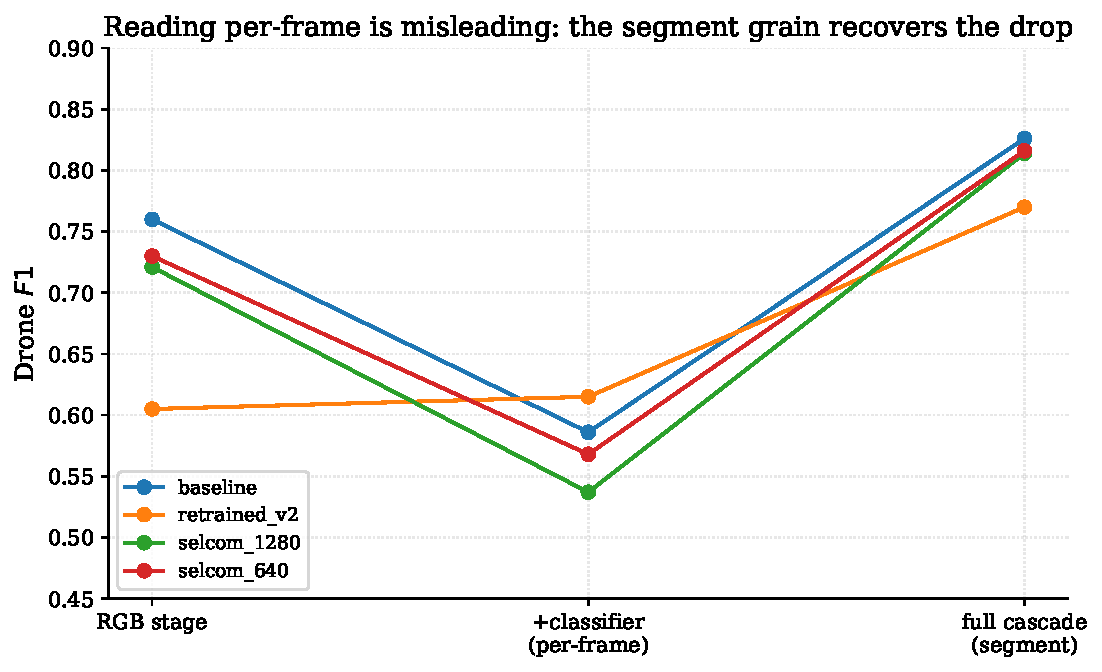
\includegraphics[width=0.75\textwidth]{fig8_perframe_segment}
    \caption{Why per-frame metrics mislead. For each RGB variant, drone $F1$ \emph{drops} when the trust classifier merges modalities at the per-frame grain, then \emph{recovers} (and exceeds the RGB stage) once the $3$-frame temporal smoother resolves alerts at the segment grain. The deployed system fires on segments, not frames, so the segment values are the production-relevant ones. Source: \textsc{Ledger}~\S9.5.}
    % [source: ledger=cascade-perframe-misleading; eval=pipe_vid_baseline_pf,pipe_vid_baseline_seg; run=(EVIDENCE_LEDGER sweep); config=pipe_video_drone_iop]
    \label{fig:perframe_segment}
\end{figure}

This is not a cascade failure; it is the wrong unit of analysis. The deployed system does not issue alerts per frame. It accumulates segment-level evidence over a 3-frame temporal window and fires an alert event on each segment that crosses the threshold. The per-frame view counts every wrong box on every frame; the production view counts \emph{alerts}.

\subsection{Segment-level metrics: cascade earns its budget}

At the segment grain, the cascade is monotonically better than the raw RGB stage for confuser fire rate while costing only modest drone-$F1$ (Table~\ref{tab:cascade_segment}). The temporal smoother is the load-bearing recovery step, it discards per-frame FPs that do not persist across the 3-frame window. The patch veto removes a further 0.7--1.4~pp of drone segment $F1$ for a 0.7--2.1~pp cut in confuser FPR.

\begin{table}[htbp]
    \centering
    \caption{Segment-level (3-frame window) drone $F1$ and all-confuser FPR. \emph{Drone $F1$ cascade}: the segment-level drone $F1$ after temporal + patch veto. \emph{Confuser FPR cascade}: the segment-level fire rate on confuser-only videos after the same stack. \emph{Cut}: relative reduction from Stage-1 RGB. The cascade absorbs detector variance, post-cascade $F1$ spans $0.770$--$0.826$ versus the Stage-1 spread of $0.605$--$0.760$. Source: \textsc{Ledger}~\S9.5.}
    \label{tab:cascade_segment}
    \begin{tabular}{lccccc}
        \toprule
        RGB model & RGB $F1$ & Cascade $F1$ & RGB FPR & Cascade FPR & FPR cut \\
        \midrule
        baseline           & 0.760 & \textbf{0.826} & 0.512 & 0.162 & $68\%$ \\
        \texttt{retrained\_v2} & 0.605 & 0.770 & 0.196 & \textbf{0.119} & $39\%$ \\
        \texttt{selcom\_1280}  & 0.721 & 0.814 & \textbf{0.709} & 0.136 & $\mathbf{81\%}$ \\
        \texttt{selcom\_640}   & 0.730 & 0.816 & 0.260 & 0.126 & $52\%$ \\
        \bottomrule
    \end{tabular}
\end{table}

\begin{figure}[htbp]
    \centering
    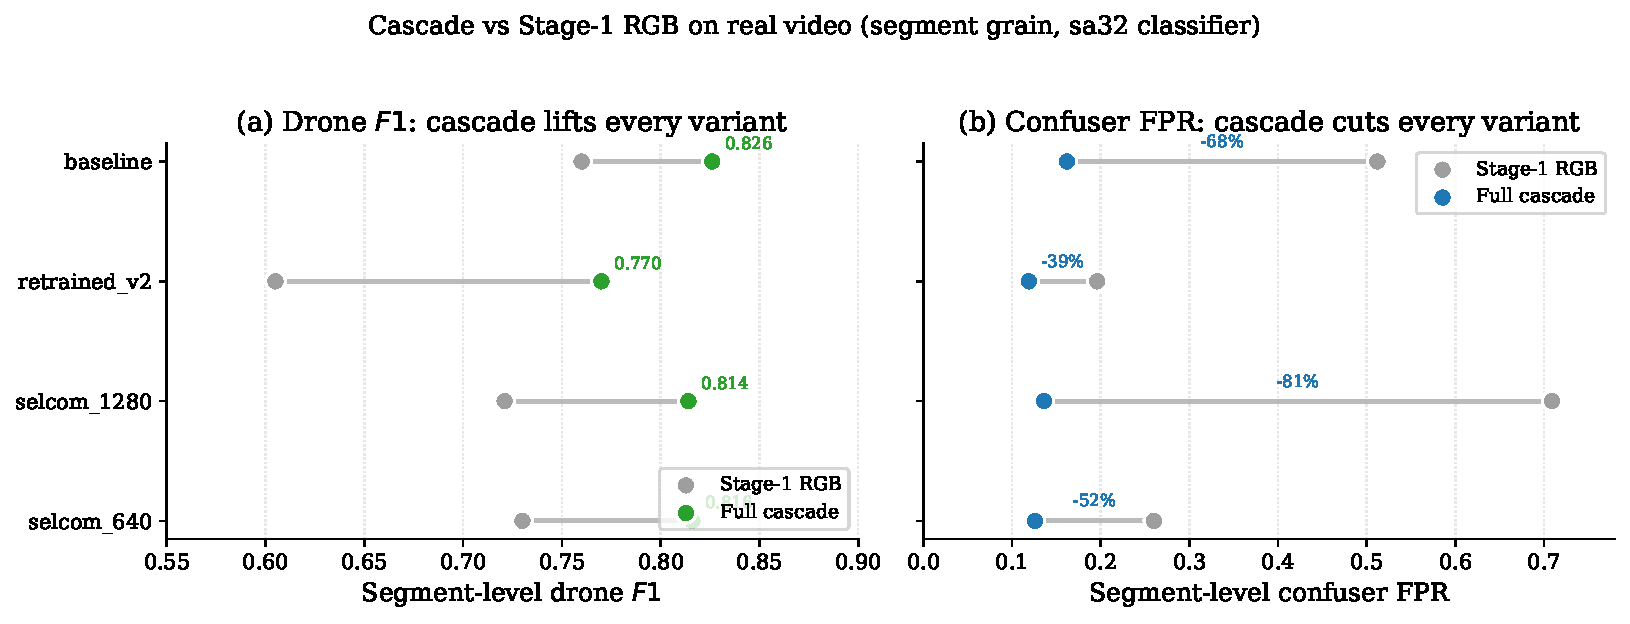
\includegraphics[width=\textwidth]{fig8_cascade_segment}
    \caption{Segment-level drone $F1$ and confuser FPR, Stage-1 RGB (grey) versus the full cascade, for the four RGB variants on the real-video diagnostic. (a) The cascade \emph{lifts} drone $F1$ for every variant ($+6.6$ to $+16.5$~pp). (b) It \emph{cuts} confuser FPR by $39$--$81\%$. The two effects together compress the Stage-1 spread (15.5~pp $F1$ / 51.3~pp FPR) to $5.6$~pp / $4.3$~pp. Source: \textsc{Ledger}~\S9.5.}
    % [source: ledger=cascade-segment-recovers; eval=pipe_vid_baseline_seg,pipe_vidconf_selcom1280_seg; run=(EVIDENCE_LEDGER sweep); config=pipe_video_drone_iop]
    \label{fig:cascade_segment_fig}
\end{figure}

\paragraph{The cascade compresses the Stage-1 spread.}
At Stage 1 the four RGB variants span 15.5~pp of drone $F1$ ($0.605$ to $0.760$) and 51.3~pp of confuser FPR ($0.196$ to $0.709$). After the full cascade those spreads tighten to 5.6~pp drone $F1$ ($0.770$ to $0.826$) and 4.3~pp confuser FPR ($0.119$ to $0.162$). The downstream stack normalises detector variance, \texttt{selcom\_1280}'s aggressive fire is suppressed, \texttt{retrained\_v2}'s conservative miss rate is lifted, and the four variants converge.
% [source: ledger=cascade-tightens-variance; eval=pipe_vid_baseline_seg; run=(EVIDENCE_LEDGER sweep); config=pipe_video_drone_iop]

\paragraph{The cascade is most valuable on the worst Stage-1 detector.}
\texttt{selcom\_1280} has the worst Stage-1 confuser FPR in the table ($0.709$, by a wide margin). After the cascade it lands at $0.136$, an 81\% relative reduction, the largest in the table. The cascade's value is exactly where the Stage-1 cost is highest. This is consistent with the design intent: the trust classifier and the patch verifier exist precisely to convert detector confidence into modality- and scene-conditional alert decisions.
% [source: ledger=cascade-segment-recovers; eval=pipe_vidconf_selcom1280_seg; run=(EVIDENCE_LEDGER sweep); config=pipe_video_confuser]

\paragraph{Drone-$F1$ cost is small at the alert grain.}
Stage-1 baseline $F1$ is $0.760$ and cascade baseline $F1$ is $0.826$: at the segment grain the cascade does not cost drone $F1$, it \emph{gains} it (temporal smoothing recovers per-frame misses that fire on neighbouring frames). For the other three RGB variants the cascade gain is even larger ($+8.5$ to $+16.5$~pp $F1$). The Svanstr\"om-paired finding that the cascade costs in-distribution F1 (\S\ref{sec:cumulative}) is therefore a Svanstr\"om-specific observation; on real video, where the per-frame Stage-1 metrics are noisier to begin with, the temporal smoother provides net recovery.
% [source: ledger=cascade-segment-recovers; eval=pipe_vid_baseline_seg; run=(EVIDENCE_LEDGER sweep); config=pipe_video_drone_iop]

\subsection{Per-category cascade suppression}
\label{sec:realvideo_percategory}

The aggregate confuser FPR in Table~\ref{tab:cascade_segment} averages across three confuser categories with very different cascade-stage behaviour. Breaking the same numbers out per category exposes which suppression the cascade is actually doing (Table~\ref{tab:cascade_percategory}).

\begin{table}[htbp]
    \centering
    \caption{Segment-level confuser FPR after temporal + patch veto, broken out by category. The cascade earns its keep on birds (a 45$\times$ suppression for \texttt{selcom\_1280}) and is essentially inert on airplanes. Source: \textsc{Ledger}~\S9.5.9.}
    \label{tab:cascade_percategory}
    \begin{tabular}{lccc}
        \toprule
        RGB model & Birds & Airplanes & Helicopters \\
        \midrule
        baseline           & 0.017 & 0.225 & 0.216 \\
        \texttt{retrained\_v2} & \textbf{0.008} & \textbf{0.206} & 0.141 \\
        \texttt{selcom\_1280}  & 0.034 & 0.216 & 0.156 \\
        \texttt{selcom\_640}   & 0.008 & 0.216 & 0.151 \\
        \bottomrule
    \end{tabular}
\end{table}

\paragraph{The cascade's value is concentrated on birds, exactly as designed.}
\texttt{selcom\_1280}'s bird FPPI of 1.528 at Stage 1 (\S\ref{sec:realvideo}, Table~\ref{tab:realvideo_master}) collapses to a 0.034 segment-level FPR after the cascade, a $45\times$ reduction at the alert grain. Baseline RGB's bird FPPI of 0.960 collapses to 0.017 ($57\times$). Birds are the category the detector cannot be trained to suppress without losing drone recall (\S\ref{sec:rgb_three_variants}); they are also the category the cascade suppresses most aggressively. This matches the architecture's stated rationale (\S\ref{sec:design_rationale}).
% [source: ledger=cascade-bird-vs-airplane-asymmetry; eval=pipe_percat_sa32; run=(EVIDENCE_LEDGER sweep); config=pipe_video_confuser]

\paragraph{The cascade is essentially inert on airplanes.}
Post-cascade airplane FPR is $\sim 0.21$ across all four RGB models, regardless of whether the Stage-1 RGB stage fired on 109 or 150 detections per video. At the per-frame measurement the trust classifier sometimes \emph{adds} airplane FPs by merging modalities (baseline 137 RGB FPs $\to$ 143 post-classifier). The patch verifier audit (\S\ref{sec:patch_audit}) had already shown the verifier is genuinely uncertain on airplane crops (median patch prob $0.540$ vs $0.904$ for birds and $0.987$ for helicopters), so a soft veto does not happen at the alert gate either. Airplane suppression is the cascade's weakest link, and the dedicated remediation is a MobileNetV3 patch-verifier retrain with explicit OOD airplane crops (distinct from the distilled \texttt{mlp\_v5} verifier of \S\ref{sec:distill_verifier}, which targets the same crops via feature reuse) (\S\ref{sec:limits}).
% [source: ledger=cascade-bird-vs-airplane-asymmetry; eval=pipe_percat_sa32; run=(EVIDENCE_LEDGER sweep); config=pipe_video_confuser]

\paragraph{Helicopters fall in between.}
15--34\% per-frame classifier suppression and modest further cuts at segment level. The cascade's selectivity on helicopters is consistent with the IR detector firing on helicopters in some scenes (helicopters have thermal signatures the IR detector partially picks up), giving the trust classifier a useful agreement signal that is absent for airplanes.
% [source: ledger=cascade-bird-vs-airplane-asymmetry; eval=pipe_percat_sa32; run=(EVIDENCE_LEDGER sweep); config=pipe_video_confuser]

The bird-vs-airplane asymmetry is the strongest single argument for the cascade's design intent: the downstream stack handles exactly the category where detector-level confuser mining hits a wall (\S\ref{sec:rgb_three_variants}), and is honest about its inability to handle the category where detector-level mining already worked.

\subsection{Classifier choice on real video}
\label{sec:realvideo_classifier}

The Svanstr\"om-side classifier comparison (\S\ref{sec:cumulative}, Table~\ref{tab:classifiers}) identified three candidates: \texttt{scene\_aware\_v3more\_32feat} (sa32), \texttt{control\_v3more\_40feat} (control40), and \texttt{fusion\_no\_fn\_v1.1} (fnfn). All three were re-evaluated on the real-video diagnostic set, each with the same RGB / IR / patch verifier configuration. The sa32 cascade above is the production-pick result; Tables~\ref{tab:cascade_classifier_drone} and \ref{tab:cascade_classifier_fpr} place it next to the two alternatives.

\begin{table}[htbp]
    \centering
    \caption{Segment-level drone $F1$ under three classifiers on the real-video diagnostic. sa32 dominates for every RGB variant; fnfn rejects 85\% of correct RGB drone TPs and collapses segment $R$ to $\leq 0.128$. Source: \textsc{Ledger}~\S9.5.8.}
    \label{tab:cascade_classifier_drone}
    \begin{tabular}{lccc}
        \toprule
        RGB model & sa32 & control40 & fnfn \\
        \midrule
        baseline           & \textbf{0.826} & 0.644 & 0.219 \\
        \texttt{retrained\_v2} & 0.770 & 0.576 & 0.181 \\
        \texttt{selcom\_1280}  & 0.814 & 0.595 & 0.108 \\
        \texttt{selcom\_640}   & 0.816 & 0.619 & 0.165 \\
        \bottomrule
    \end{tabular}
\end{table}

\begin{table}[htbp]
    \centering
    \caption{Segment-level all-confuser FPR under three classifiers. fnfn cuts the FPR to 1.2--2.4\%, but at the drone-recall cost shown in Table~\ref{tab:cascade_classifier_drone}. Source: \textsc{Ledger}~\S9.5.8.}
    \label{tab:cascade_classifier_fpr}
    \begin{tabular}{lcccc}
        \toprule
        RGB model & RGB raw & sa32 & control40 & fnfn \\
        \midrule
        baseline           & 0.512 & 0.162 & 0.083 & \textbf{0.024} \\
        \texttt{retrained\_v2} & 0.196 & 0.119 & 0.045 & 0.012 \\
        \texttt{selcom\_1280}  & 0.709 & 0.136 & 0.057 & 0.019 \\
        \texttt{selcom\_640}   & 0.260 & 0.126 & 0.040 & 0.021 \\
        \bottomrule
    \end{tabular}
\end{table}

\begin{figure}[htbp]
    \centering
    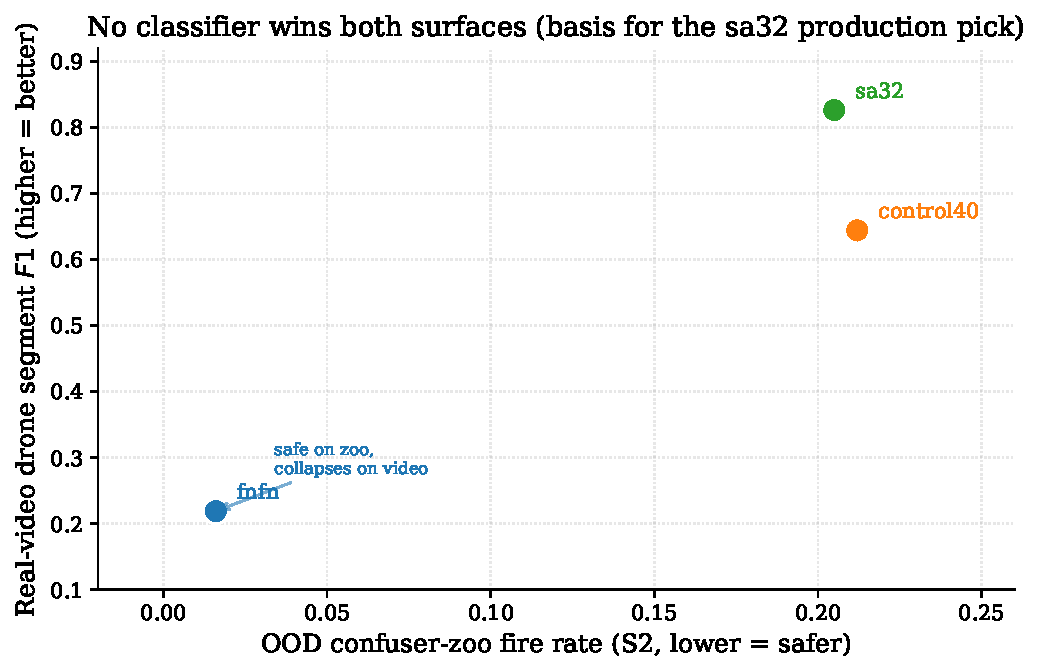
\includegraphics[width=0.7\textwidth]{fig8_classifier_reversal}
    \caption{No trust classifier wins both surfaces. On the OOD confuser zoo \texttt{fusion\_no\_fn\_v1.1} is far the safest (S2 fire $0.016$) but on real video it collapses drone $F1$ to $0.219$; \texttt{sa32} inverts the ranking, dominating real-video drone $F1$ ($0.826$) at a higher zoo fire ($0.205$). The Svanstr\"om/zoo ordering does not by itself select the production classifier --- this surface reversal motivated the \texttt{sa32} working pick, later superseded by the statistically-derived \texttt{robust6}/\texttt{robust8} (\S\ref{sec:feature_selection}). Source: \textsc{Ledger}~\S7, \S9.5.8.}
    % [source: ledger=three-classifier-realvideo; eval=pipe3clf_sa32,pipe3clf_fnfn,clfzoo_fnfn; run=(EVIDENCE_LEDGER sweep); config=pipe_video_drone_iop]
    \label{fig:classifier_reversal}
\end{figure}

\paragraph{The Svanstr\"om classifier ordering is partly Svanstr\"om-specific.}
\S\ref{sec:cumulative} (Table~\ref{tab:classifiers}) found three classifiers within 1.3~pp of each other on Svanstr\"om drone $F1$ and a sharper split between fnfn (S2 zoo fire 0.016) on one side and sa32/control40 (both $\approx 0.21$ S2, $\approx 0.10$ S3) on the other. On real-video the ordering changes: sa32 dominates drone $F1$ (0.826 baseline), control40 sits 18~pp behind on drone $F1$ at the same RGB stage, and fnfn collapses drone recall below operational viability. The Svanstr\"om benchmark therefore does not by itself select the production classifier.
% [source: ledger=three-classifier-realvideo; eval=clfzoo_sa32; run=eval/cumulative_halluc.py; cache=eval/results/_cumulative_halluc/confuser_sa32/summary.json; config=confuser_zoo_1280]

\paragraph{fnfn is too conservative for real-video deployment.}
fnfn accepts only 15\% of the RGB stage's correct drone TPs (136 of 924 for baseline RGB on the per-frame measurement); segment-level drone $R$ falls to $0.128$. For an alert system this is the same as missing seven out of eight drone events. fnfn remains a valid open-world fallback when missed drones are operationally cheaper than confuser-induced false alarms; on the surface tested here, the trade is unfavourable.
% [source: ledger=three-classifier-realvideo; eval=pipe3clf_fnfn; run=(EVIDENCE_LEDGER sweep); config=pipe_video_drone_iop]

\paragraph{control40 buys nothing over sa32.}
control40 ties sa32 on Svanstr\"om within 1.3~pp drone $F1$ (\S\ref{sec:classifier_compare}, Table~\ref{tab:classifiers}) and ties it on the OOD confuser zoo within rounding (S2 0.212 vs 0.205; S3 0.094 vs 0.103). On real-video, however, control40 loses 18~pp drone segment $F1$ to sa32 (0.826 $\to$ 0.644) and only cuts confuser FPR from 0.162 to 0.083, a 49\% reduction that is also achievable downstream by raising \texttt{patch\_thr} without paying the drone-recall cost. There is no operational regime in the measured surfaces where control40 strictly outperforms sa32 on the joint axis. Within this hand-assembled comparison set \texttt{sa32} is therefore the winner, with \texttt{fusion\_no\_fn\_v1.1} retained as the open-world fallback and \texttt{control\_v3more\_40feat} deprecated. \texttt{sa32} is, however, the \emph{comparison} pick, not the shipped classifier: it was trained on detections from the superseded \texttt{selcom\_1280} detector and on per-frame scene-statistic features that leak scene identity. The production classifier is the six-feature leakage-aware \texttt{robust6}, re-mined on the \texttt{ft4}/\texttt{v3b} detectors and selected statistically rather than by hand (\S\ref{sec:feature_selection}, Table~\ref{tab:robust6_pipeline}); it matches \texttt{sa32} in-domain and is materially more robust on OOD confusers.
% [source: ledger=trust-classifier-conditional; eval=svan_s3_sa32_thr08; run=(EVIDENCE_LEDGER sweep); config=svan_iop_1280_s9]

\subsection{Pinned open items}
Two runs are registered against this section (\textsc{Ledger}~\S9.5.7) and acknowledged as future work rather than thesis-time gaps:
\emph{(i)} include \texttt{flock\_of\_birds\_attack\_drone} (the Stage-1 case where baseline and \texttt{retrained\_v2} score $F1=0$ and only \texttt{selcom\_1280} detects the drone, \S\ref{sec:realvideo}) so the cascade's behaviour on the hardest bird-vs-drone confounder is measured as a visceral single-case demonstration; \emph{(ii)} a real-video patch-threshold sweep, analogous to the Svanstr\"om sweep in \S\ref{sec:patch_threshold}, to confirm the production \texttt{patch\_thr} on this surface (currently 0.7 for real-video, 0.9 for Svanstr\"om). The Svanstr\"om sweep was monotone in the useful range, so the real-video sweep is expected to confirm rather than redirect.

\section{SelCom CCTV Evaluation}
\label{sec:selcom}

The SelCom CCTV fine-tune was introduced in \S\ref{sec:selcom_finetune}. The full evaluation grid is recorded in \textsc{Ledger}~\S3.4; the production weights are \texttt{Yolo26n\_selcom\_mixed\_ft2\_1280}. The two key empirical findings are: (i) doubling \texttt{imgsz} from 640 to 1280 doubles selcom recall \emph{and} raises precision, which is not a recall--precision trade-off but a genuine resolution win on small drones; (ii) no OpenCV preprocessing variant in the sweep improved selcom detection independently of fine-tuning and \texttt{imgsz}; among the levers tested, fine-tuning and resolution were the effective ones. The imgsz sweep further identifies \texttt{imgsz=960} as the F1-optimal CCTV operating point in clutter-bound conditions (\texttt{docs/analysis/2026-05-16\_rgb\_camera\_spec\_and\_fault\_profile.md}).

Evaluated at \texttt{imgsz=960}, this SelCom fine-tune (\texttt{selcom\_960}) is in fact the best \emph{cross-surface} drone-first RGB variant tested (composite rank $2.5$): it leads on the SelCom hold-out ($F1=0.585$, vs \texttt{selcom\_1280}'s $0.580$ and the baseline's $0.15$) and on the Roboflow OOD drone split with the patch verifier ($F1=0.84$, vs baseline $0.79$). It is deliberately \emph{not} in the production stack: it loses to the baseline on Svanstr\"om medium-range drones and on clean video, and it has not been run through the full cascade. It is recorded here as a candidate to revisit, not a settled recommendation.
% [source: ledger=selcom960-cross-surface-winner; eval=xsurf_selcom_holdout,xsurf_roboflow_drone; run=(EVIDENCE_LEDGER sweep); config=selcom_holdout_persize]

\section{Threats to Validity}
\label{sec:threats}

\paragraph{Internal validity.}
Three threats. First, the RGB detector's three training stances (\S\ref{sec:rgb_three_variants}) and the patch verifier's four versions (\S\ref{sec:patch_verifier_arch}) were iterated against Svanstr\"om evaluation results; some design decisions are therefore implicitly biased toward Svanstr\"om performance. The Roboflow OOD audit (\S\ref{sec:roboflow}) is the partial mitigation. Second, \texttt{imgsz} acts as a hidden hyperparameter: Svanstr\"om drone recall is $R=0.961$ at \texttt{imgsz=1280} but collapses below the resolvable floor at \texttt{imgsz=640} ($R=0.072$, measured on \texttt{retrained\_v2}; \S\ref{sec:resolution_arch}). All Svanstr\"om \emph{RGB} numbers in this thesis use \texttt{imgsz=1280} consistently; the IR detector is evaluated at its native \texttt{imgsz=640} ($640{\times}512$ thermal), where the RGB small-drone resolution collapse does not apply. Third, the trust classifier was trained against a specific RGB confidence calibration, and swapping the RGB detector (e.g., from baseline to a future selcom-fine-tune) without re-evaluating the classifier risks silent degradation; this is recorded in \textsc{Ledger}~\S5 (classifier-RGB pairing).
% [source: ledger=v5-selcom-train-deploy-mismatch; eval=clf3_retrainedv2; run=eval/eval_classifier_3way.py; cache=docs/analysis/full_pipeline_ablations/csv/classifier_3way.csv; config=clf_3way_300]

\paragraph{Construct validity.}
IoP at threshold 0.5 is more lenient than IoU at the same threshold for small-object detection. Numbers in this thesis are therefore not directly comparable to IoU-based numbers in the literature without an explicit conversion. The rule is justified operationally (the cascade's downstream stages consume detection crops) but is non-standard. The scoring-rule audit (\S\ref{sec:scoring_audit}) raises a related but distinct issue: trust-aware vs dual scoring of identical detections swings F1 by 28~pp, and any literature comparison must check the scoring rule used.

\paragraph{External validity.}
The trust classifier was trained on all 28,710 Svanstr\"om frames using a sequence-stratified split; the cascade-level evaluation in this chapter runs on those same frames. Approximately 22,000 of the 28,710 frames overlap with the classifier's training partition. Svanstr\"om cascade numbers are therefore in-distribution upper bounds. The Anti-UAV cascade numbers are fully clean. The IR detector was trained on 18,639 centre-zoomed Svanstr\"om crops (\texttt{IR\_dset\_final/train}), so Svanstr\"om IR numbers are also in-distribution; the IR Svanstr\"om F1$=$0.961 is consistent with the IR Anti-UAV F1$=$0.965, which suggests the overlap does not meaningfully inflate the reported figure but should be noted.
% [source: ledger=prov-may10-imgsz; eval=ir_v3b_svan640_may10; run=(May-10 ablation matrix); cache=eval/results/_ablation/2026-05-10T16-08-14/master.csv; config=svan_iop_640_may10]

A final caveat concerns sample size on the real-video diagnostic. Per-clip confuser FPPI is computed from only $\sim$20--340 sampled frames per clip (Appendix~\ref{app:datasets}), so the per-category figures of \S\ref{sec:realvideo_percategory} and individual per-clip rates carry wide sampling error. The aggregate confuser numbers (1{,}250 frames across 10 clips) are the reliable quantities, and single-clip values such as the bird-FPPI ratios should be read as indicative rather than precise.

\paragraph{Conclusion validity.}
The strength of the statistical inference varies across the comparisons, and the language is calibrated to match. The real-video confuser figures are reliable in aggregate ($1{,}250$ frames over $10$ clips) but thin per category ($20$--$340$ frames per clip), so individual per-clip ratios are indicative rather than precise (\S\ref{sec:realvideo}). The grayscale cross-modal result is reported as a tie on a single bird-cluttered clip, not a win (\S\ref{sec:grayscale}). The \texttt{robust8} grayscale-recall gain is the one comparison carrying a bootstrap confidence interval; the surrounding full-pipeline numbers are single-run point estimates without repeated-seed variance, so differences within roughly $1$--$2$~pp are treated as ties throughout, consistent with typical run-to-run variation on these surfaces.
% [source: ledger=robust8-grayscale-router,ir-grayscale-fallback; eval=svan_gray_robust8_t20_clffilter; run=eval/compare_routing_pipeline.py; cache=eval/results/_routing_pipeline_cmp/comparison.md]

\paragraph{Resolution and modality confounds.}
Three comparisons hold a resolution or modality variable unequal and should be read with that in mind. First, the ``\texttt{imgsz=640} is unusable'' generalisation is measured on the worst-case \texttt{retrained\_v2} variant ($R=0.072$); a baseline-detector @640 evaluation was not run, so the claim is bounded to that variant rather than to every RGB detector. Second, the observation that IR edges RGB on Svanstr\"om compares IR at its native $640$ against RGB at $1280$, so the $1.1$-pp IR margin sits inside the resolution difference; the load-bearing claim is the \emph{different hallucination profiles} of the two modalities, which needs no superiority result. Third, the \texttt{robust6}/\texttt{robust8} ``$\sim$30\% fewer false alerts'' rests on an evaluation whose drone positives use thermal IR while the confuser negatives use grayscale-fallback IR --- a modality split across the two classes in the classifier's IR features --- so it is reported with that caveat rather than as a pure architectural effect.
% [source: ledger=robust6-production-viable; eval=clf_own_holdout; run=eval/overnight_ablation.py; cache=eval/results/_overnight_ablation/ablation_results.json; config=clf_own_holdout]

\section{Limitations and Future Work}
\label{sec:limits}

\paragraph{Latency.}
All evaluation in this thesis was performed on a GTX 1050~Ti (4~GB VRAM) development GPU. Latency on production-grade edge hardware (NVIDIA Jetson Orin / Xavier) is not measured. The production cascade adds sequential inference stages (RGB YOLO, IR YOLO, the \texttt{robust8} XGBoost classifier --- eight free detector-output features with no per-frame scene reads, roughly $400\times$ cheaper per frame than the scene-statistic classifiers it replaces --- and the two small per-frame MLP verifiers, which reuse detector features and are $46$--$72\times$ cheaper per detection than the superseded MobileNetV3 patch verifier); on the GTX~1050~Ti the full cascade runs interactively under the PySide6 GUI, but interactive is not the same as real-time on Jetson, and the latency budget is one of the remaining production-readiness checks.
% [source: ledger=robust6-speed-feature-efficiency,v5-ship-per-frame; eval=clf_own_holdout; run=eval/bench_speed.py; cache=docs/analysis/2026-06-04_consolidated_sell_new_stack.md; config=clf_own_holdout]

\paragraph{Temporal smoother credit.}
The frame-independent evaluation harness omits the temporal smoother to keep per-stage credit clean. The deployed system uses an $N$-of-$M$ smoother (\S\ref{sec:temporal}) that contributes additional confuser rejection in real video. The cumulative-suppression numbers in \S\ref{sec:cumulative} are therefore lower bounds on the deployed system's confuser rejection.

\paragraph{Patch verifier and OOD airplanes.}
The patch verifier (predecessor to the production \texttt{mlp\_v5}, \S\ref{sec:distill_verifier}) suppresses 50--52\% of bird FPs across both modalities but only 2--7\% of OOD airplanes (\S\ref{sec:roboflow}). The verifier is trained on Svanstr\"om-scale confuser crops; large, in-frame airplanes are out of distribution. The distilled \texttt{mlp\_v5} that supersedes it inherits the same OOD-airplane exposure gap, so the recommended remediation applies to both: documented in \texttt{path\_forward.md} \S3b, collect the specific Roboflow airplane FP crops as confuser-class training data.
% [source: ledger=patch-verifier-distribution-bound; eval=rob_rgb_baseline; run=eval/run_roboflow_eval.py; config=roboflow_rgb_drone_640]

\paragraph{IR brittleness on OOD.}
The IR detector reaches $R \geq 0.94$ on in-distribution data (Anti-UAV, Svanstr\"om IR) but $R=0.519$ on \texttt{ir\_mixed\_cbam} and $R=0.264$ on \texttt{ir\_drone\_night} (\S\ref{sec:roboflow}). The latter is partly augmentation-induced, but the former is a real generalisation gap. The IR detector is the single weakest link in the OOD regime.
% [source: ledger=ir-ood-recall-ceiling; eval=ir_ood_cbam_raw; run=(EVIDENCE_LEDGER sweep); config=roboflow_ir_drone_640]

\paragraph{Drone-trajectory classification.}
The temporal smoother maintains a per-track state and renders a drone-path visualisation in the GUI, but does not yet use track-level features (velocity, acceleration, persistence) as classifier input. Drones, birds, and aircraft have distinct flight dynamics, so a track-based classifier would add a fourth, largely orthogonal evidence channel to the cascade --- a promising direction for the airplane-suppression gap (\S\ref{sec:realvideo_percategory}) that the appearance-based stages cannot close.

\paragraph{Open ledger items.}
The open items the thesis carries forward at the time of writing are: end-to-end latency on edge hardware (\textsc{Ledger}~\S10), a real-video patch-threshold sweep analogous to \S\ref{sec:patch_threshold} (currently \texttt{patch\_thr=0.7} was used for real-video, while Svanstr\"om uses \texttt{patch\_thr=0.9}), per-category cascade confuser FPR breakdowns from the per-video JSONs, and the \texttt{flock\_of\_birds\_attack\_drone} cascade case (\S\ref{sec:realvideo}, \S\ref{sec:realvideo_cascade}). The previously-open \texttt{control\_v3more\_40feat} OOD-zoo measurement is resolved (\S\ref{sec:classifier_compare}, Table~\ref{tab:classifiers}), as is the grayscale IR confuser provenance (\textsc{Ledger}~\S9.4 supersedes the earlier \S4 UNKNOWN).

% ======================================================================
% CHAPTER 7 — CONCLUSION
% ======================================================================
\chapter{Conclusion}
\label{ch:conclusion}

This thesis presented a multi-stage drone detection architecture in which the base detector is tuned for recall and confuser discrimination is handled by downstream learned stages. The design was validated component by component against a set of comparison variants and ablations, and the production stack (\S\ref{sec:production_stack}) is the integration of the winning component at each stage, and the quantitative claims are registered in the evidence ledger against the commands that produced them.

\section{Answers to the Research Questions}
\label{sec:rq_answers}

\paragraph{RQ1 (cascade confuser-suppression).}
\emph{Yes.} In the classifier-comparison configuration (baseline RGB, v2 patch verifier; \S\ref{sec:cumulative}), the cascade reduces OOD confuser fire rate from 52.1\% (RGB detector alone) to 10.3\% with \texttt{scene\_aware\_v3more\_32feat} and to 0.8\% with the open-world \texttt{fusion\_no\_fn\_v1.1} (Table~\ref{tab:cum_confuser}). Hard-negative mining at the detector stage achieves at most $66.2\% \to 41.9\%$ on helicopters and is essentially inert on birds at small scale ($94.4\% \to 94.2\%$, \S\ref{sec:rgb_three_variants}). The cascade therefore catches what the detector cannot, without requiring the detector itself to be retrained against the bird category at unacceptable recall cost. The leakage-aware \texttt{robust6} classifier --- and its shipped grayscale-hardened extension \texttt{robust8} --- reproduces this suppression on the current \texttt{ft4}/\texttt{v3b} detectors --- on an unseen confuser surface it cuts the classifier-only false-alert rate to $0.143$ and the best-composed cascade to $0.057$ (\S\ref{sec:feature_selection}, Table~\ref{tab:robust6_pipeline}) --- using six leakage-free features in place of \texttt{sa32}'s $32$.
% [source: ledger=cascade-confuser-collapse; eval=clfzoo_fnfn; run=eval/cumulative_halluc.py; cache=eval/results/_cumulative_halluc/confuser_fusion_no_fn_model_v1.1/summary.json; config=confuser_zoo_1280]

\paragraph{RQ2 (in-distribution cost and surface dependence).}
\emph{Surface-dependent, not architecture-intrinsic.} The comparison configuration that establishes this (baseline RGB, \texttt{sa32}, v2 patch verifier) shows the sign of the exchange flip with the surface. On Svanstr\"om paired data the cascade trades drone $F1$ for OOD safety: S1 $F1=0.950$ falls to S3 $F1=0.895$ at \texttt{patch\_thr}$=0.9$ (\S\ref{sec:patch_threshold}, Table~\ref{tab:patch_sweep}). On the real-video diagnostic the same cascade with the same classifier and temporal smoother gains $F1$ over the Stage-1 RGB number ($0.760 \to 0.826$ for baseline RGB) while still cutting confuser FPR threefold (\S\ref{sec:realvideo_cascade}, Table~\ref{tab:cascade_segment}). The classifier choice is load-bearing: \texttt{fusion\_no\_fn\_v1.1} collapses real-video drone recall to $R=0.128$ while \texttt{scene\_aware\_v3more\_32feat} preserves it (\S\ref{sec:realvideo_classifier}). The exchange is therefore a joint property of the classifier and the evaluation surface, not of the cascade architecture. The production stack carries the same conclusion forward with the leakage-aware \texttt{robust8} classifier and the per-frame \texttt{mlp\_v5}/\texttt{mlp\_v5\_ir\_aligned} verifiers (\S\ref{sec:production_stack}); the full-cascade real-video re-run with those production verifiers in the alert-gate slot is a registered open item (Figure~\ref{fig:mlp_pipeline_placeholder}).
% [source: ledger=cascade-segment-recovers; eval=svan_s3_sa32_thr08; run=(EVIDENCE_LEDGER sweep); config=svan_iop_1280_s9]

\paragraph{RQ3 (cross-study comparability and scoring).}
\emph{Limited; explicit scoring disclosure is necessary.} The scoring-rule audit of \S\ref{sec:scoring_audit} documents a 28-percentage-point F1 swing between dual and trust-aware aggregation of identical detections on Svanstr\"om, independently of the IoU/IoP choice. The IoP/IoU axis is the second comparability hazard. Numerical comparison to prior work on Svanstr\"om and Anti-UAV (Chapter~\ref{ch:literature}, Table~\ref{tab:numerical_comparison}) survives only at the qualitative level: this thesis's per-modality detectors are in the same range as published baselines, but multi-modal headline numbers cannot be compared across studies without explicit scoring disclosure.

\paragraph{RQ4 (cross-modal transfer).}
\emph{Partially --- the transfer holds where the discriminative content is silhouette-shaped, and degrades where it is not.} The IR detector, trained zero-shot on thermal data only, reaches drone $F1=0.636$ on grayscale-converted RGB video aggregate and $F1=0.837$ on the hardest bird-cluttered single clip (\S\ref{sec:grayscale}, Tables~\ref{tab:ir_grayscale}, \ref{tab:realvideo_seagull}), tying the strongest RGB detector at $F1=0.840$ on that clip while cutting confuser FPPI by $3.2\times$ aggregate ($0.512 \to 0.158$). The transfer is preserved by the single-channel intensity input; the raw-3-channel-RGB control collapses to $F1=0.295$, isolating the grayscale conversion as the load-bearing step. The transfer is partial: on clean drone takeoff clips the dedicated RGB detectors win by 28--41~pp $F1$. The pattern is consistent with a detector that has learned silhouette structure strongly and visible-light texture weakly.
% [source: ledger=ir-grayscale-fallback; eval=vid_drone_ir_gray; run=eval/eval_video_tests.py; config=video_drone_iop]

\paragraph{Methodological thread (HITL co-development).}
The IR detector's precision / recall trajectory across six revisions on a fixed test split (Table~\ref{tab:ir_evolution}) characterises the dataset-state $\leftrightarrow$ model-state coupling. The V5 regression ($P: 0.895 \to 0.768$) is the case the protocol got wrong: a large batch of positives was injected in bulk instead of through the per-batch review loop, so the unreviewed batch carried unlabelled drones that V5 fires on as scored-FP. V6 and \texttt{Final} recover the precision by corpus cleanup. Reporting the regression is informative because it identifies a failure mode of HITL ingestion that is easy to repeat.
% [source: ledger=ir-version-progression; eval=ir_final_v5; run=eval/ir_version_comparison.py; cache=eval/results/ir_version_comparison/ir_comparison_test_640_2026-05-16T20-04-39.csv; config=ir_final_640]

\section{Production Stack and Future Work}
\label{sec:production_stack}


The findings are summarised in the four RQ answers above (\S\ref{sec:rq_answers}) and need not be repeated in narrative form here. The methodological consequence that survives independently of any single number is that multi-modal drone-detection results are not comparable across studies without explicit scoring-rule disclosure (RQ3); the headline number swing the audit documents (28~pp $F1$ on Svanstr\"om for identical underlying detections) is larger than the inter-system differences typically debated in the literature.

The production stack as of the time of writing is as follows. The RGB detector is the SelCom-plus-confuser fine-tune \texttt{Yolo26n\_selcom\_confuser\_ft4\_1280} (\texttt{ft4}), the only confuser-injection configuration that passed every drone-recall regression gate (\S\ref{sec:training_recipes}); the earlier RGB variants --- the \texttt{Yolo26n\_trained} baseline, \texttt{hardneg\_v3more}, \texttt{retrained\_v2}, and the \texttt{selcom\_mixed\_ft2\_1280}/\texttt{selcom\_960} fine-tunes --- are comparison points that motivated this pick (\S\ref{sec:rgb_three_variants}, \S\ref{sec:selcom}), not co-deployed models.

The IR branch is the \texttt{v3b} detector (\S\ref{sec:ir_evolution}), with a grayscale-RGB fallback path (\S\ref{sec:ir_grayscale_mode}) when no thermal camera is available and, on bird-cluttered scenes, a parallel detection channel even when thermal is available. Frame-level fusion uses the eight-feature leakage-aware trust classifier \texttt{robust8} (\S\ref{sec:feature_selection}) --- the six-feature \texttt{robust6} extended with \texttt{rgb\_mean\_conf}, an \texttt{is\_grayscale} flag, and a per-class \texttt{trust\_rgb} threshold ($\tau{=}0.20$) --- re-mined on the production \texttt{ft4}/\texttt{v3b} detectors and selected by the statistical leakage analysis; the $32$-feature \texttt{scene\_aware\_v3more\_32feat} (\texttt{sa32}), \texttt{control\_v3more\_40feat}, \texttt{fusion\_no\_fn\_v1.1}, and the base \texttt{robust6} are the comparison set against which \texttt{robust8} was validated (\S\ref{sec:classifier_compare}, \S\ref{sec:feature_selection}). The confuser verifier is the distilled \texttt{mlp\_v5} on the RGB branch and its cross-modal counterpart \texttt{mlp\_v5\_ir\_aligned} (one network, two per-modality scalers; \S\ref{sec:grayscale_verifier}) on the IR branch, both running per-frame in the deployed \texttt{MLPVerifier} and superseding the MobileNetV3 v2 patch verifier (\S\ref{sec:distill_verifier}) they beat on every confuser-rich surface and both modalities (\textsc{Ledger}~mlp-beats-patch-both-modalities). The two verifiers are composed trust-classifier-first (classifier$\to$verifier), the order that is most recall-safe at equal confuser suppression (\textsc{Ledger}~robust6-production-viable). The superseded patch verifier (at \texttt{patch\_thr=0.9} Svanstr\"om / $0.7$ real-video) remains the documented fallback on the photo-style \texttt{rgb\_dataset} surface where the MLP still trails (\S\ref{sec:distill_verifier}), and the full-cascade real-video numbers in this thesis were measured with it pending the \texttt{mlp\_v5} re-run (\S\ref{sec:realvideo_cascade}, Figure~\ref{fig:mlp_pipeline_placeholder}). In the production design the \texttt{mlp\_v5}/\texttt{mlp\_v5\_ir\_aligned} verifiers run \emph{per-frame} (always-on, reusing the detector's own ROI features; \textsc{Ledger}~v5-ship-per-frame); the \texttt{alert\_gate\_only} composition under which the real-video full-cascade numbers were measured is the as-measured \emph{patch}-verifier configuration noted above, pending the \texttt{mlp\_v5} re-run (Figure~\ref{fig:mlp_pipeline_placeholder}). Inputs are scored at \texttt{imgsz=1280} on Svanstr\"om-like content and \texttt{imgsz=960} on SelCom CCTV. Trust-aware scoring is the reporting rule.
% [source: ledger=robust8-grayscale-router,mlp-beats-patch-both-modalities,v5-ship-per-frame,ir-version-progression; eval=clf_own_holdout,svan_gray_robust8_t20_clffilter; run=eval/compare_routing_pipeline.py; config=clf_own_holdout]

Three honest carve-outs accompany the stack: \texttt{robust6}'s IR and cross-modal features go to chance on the grayscale-fallback path, which is why the shipped \texttt{robust8} adds \texttt{rgb\_mean\_conf} and a per-class \texttt{trust\_rgb} threshold to recover grayscale recall there, at a measured real-video-confuser-fire cost (\textsc{Ledger}~robust8-grayscale-router, robust6-grayscale-ir-features-dead); \texttt{mlp\_v5} costs recall on the photo-style \texttt{rgb\_dataset} surface (\S\ref{sec:mlp_recall_drop}); and on grayscale the aligned IR verifier over-vetoes, so the grayscale path is gated rather than run unconditionally per-frame (\textsc{Ledger}~grayscale-trust-classifier-degrades). Latency on edge hardware (Jetson-class) is not yet measured; this and the real-video patch-threshold sweep are the open production-readiness items (the classifier-side grayscale routing hole is closed by \texttt{robust8}, \S\ref{sec:feature_selection}).
% [source: ledger=v5-ship-per-frame,robust8-grayscale-router,robust6-production-viable,mlp-beats-patch-both-modalities,ft4-backbone-freeze,ir-version-progression; eval=clf_own_holdout,svan_gray_robust8_t20_clffilter; run=eval/overnight_ablation.py,eval/compare_routing_pipeline.py; cache=eval/results/_overnight_ablation/ablation_results.json; config=clf_own_holdout]

Four future-work directions. A track-based classifier consuming the temporal smoother's per-track state as a fourth evidence channel (the most promising single direction); closing the 2--7\% OOD-airplane gap with explicit Roboflow airplane crops as confuser-class data, a remediation that applies to the distilled \texttt{mlp\_v5} as much as to the superseded patch verifier; a grayscale-aware routing gate for the \texttt{mlp\_v5\_ir\_aligned} verifier, which still over-vetoes on grayscale (\textsc{Ledger}~grayscale-trust-classifier-degrades) even though the classifier-side grayscale hole is now closed by \texttt{robust8} (\textsc{Ledger}~robust8-grayscale-router); and edge-hardware latency benchmarking with TensorRT/ONNX quantisation. The open-world \texttt{fusion\_no\_fn\_v1.1} classifier remains a deployment-profile option for surfaces where confuser noise dominates and missed drones are operationally tolerable (\S\ref{sec:realvideo_classifier}), selectable in place of the default \texttt{robust8}.
% [source: ledger=patch-verifier-distribution-bound; eval=rob_rgb_baseline; run=eval/run_roboflow_eval.py; config=roboflow_rgb_drone_640]

% ======================================================================
% APPENDIX A — DATASETS
% ======================================================================
\appendix

\chapter{Datasets in Detail}
\label{app:datasets}

This appendix consolidates the per-source / per-clip dataset metadata that the methodology chapter summarises. Numbers come from the dataset YAMLs (\texttt{rgb\_dataset/dataset.yaml}, \texttt{IR\_dset\_final/dataset.yaml}), the documentation file shipped with the confuser corpus (\texttt{rgb\_confusers\_merged/dataset\_documentation.md}), the Svanstr\"om paired-corpus meta file, and the YouTube extraction manifests.

\section{Composite RGB Training Corpus}

The full distribution by source prefix is given in Table~\ref{tab:ds_rgb_components}; the split policy is 80 / 10 / 10 with sequence-disjoint partitioning where the source did not already supply its own splits. Six negative-source rows (VIRAT, UA-DETRAC, BDD100K) contribute the 21.9\% background-negative fraction. The AirBird subset (10{,}000 images) is the bird hard-negative channel the baseline detector relies on; the composite corpus does not contain Svanstr\"om bird / airplane / helicopter splits, which are therefore OOD at evaluation time.
% [source: dataset=rgb_dataset; file=rgb_dataset/dataset.yaml]

\section{Confuser Hard-Negative Corpus}

Per-source composition is in Table~\ref{tab:ds_confusers}. Split policy:

\begin{itemize}
    \item \textbf{Sources with existing splits} (Airplane Roboflow, New\_Dataset Roboflow): original train / valid / test partitions preserved.
    \item \textbf{Sources without splits}: split by video / sequence ID at 80 / 10 / 10 to prevent leakage.
    \begin{itemize}
        \item Svanstr\"om: 165 video sequences split by sequence ID.
        \item raihanrsd: 58 video folders split by folder.
        \item Helicopter Kaggle: 20 hash-based pseudo-groups.
    \end{itemize}
    \item \textbf{Mislabeled frame removal}: 10 frames in the airplane / New\_Dataset sources contained visible drones and were excised before training.
\end{itemize}

\noindent The mined-hard-negative process for \texttt{retrained\_v2} ran the baseline detector on every confuser image and kept the 11{,}729 frames (43.4\%) on which the baseline fired; those mined frames were merged with the composite RGB corpus to produce the final 183{,}751-image \texttt{retrain\_dataset}. \texttt{hardneg\_v3more} differs in using a smaller, less aggressive merge.
% [source: dataset=rgb_confusers_merged; file=rgb_confusers_merged/dataset_documentation.md]

\section{IR Detector Corpus}

The per-prefix distribution is in Table~\ref{tab:ds_ir_components}. The Svanstr\"om IR partition (\texttt{svan}, 21{,}637 frames) is the largest single Svanstr\"om appearance in any training corpus in this thesis and is the reason Svanstr\"om IR evaluation is in-distribution for the IR detector (Table~\ref{tab:svanstrom_audit}). The corpus state documented here is the state at the \texttt{Final} checkpoint; the V2--V6 revision history (\S\ref{sec:ir_evolution}) operated on smaller predecessor variants of the same source families.

\section{Svanstr\"om Paired}

28{,}710 frames, sampled at stride~3 from 279 source video sequences. Per-class instance counts: drone 11{,}695; airplane 6{,}090; bird 5{,}298; helicopter 5{,}627. Native resolution $640{\times}512$ (RGB) with a co-registered IR channel at the same resolution. Annotators drew loose boxes around small drones, motivating the IoP@0.5 scoring rule of \S\ref{sec:metrics}.

\section{Anti-UAV RGBT}

The converted YOLO test + val splits used for evaluation comprise 85{,}374 paired frames at $1920{\times}1080$ (RGB) and $640{\times}512$ (IR). Anti-UAV is a tracking benchmark in its native form; the per-frame detection evaluation reported in this thesis is computed by re-scoring the tracking benchmark's frame-level GT boxes with the IoU@0.5 matching rule.

\section{SelCom CCTV}

Single-camera source: fixed perimeter installation, HEVC 7~Mbps stream, \texttt{yuvj420p}, $1920{\times}1080$, 25~fps. Source clip $\sim$1:30, 2{,}076 extracted frames (1{,}953 positive + 123 explicit negative). Median drone $\sqrt{\text{area}} \approx 36.8$~px in the native frame (so $\sim$12~px at \texttt{imgsz=640}, $\sim$24~px at \texttt{imgsz=1280}). The 80 / 20 train / val split (20\% pure-SelCom validation, seed~0) is preserved across the \texttt{ft1} / \texttt{mixed\_ft1} / \texttt{mixed\_ft2} / \texttt{mixed\_ft2\_1280} variants; the strongest CCTV-evaluated fine-tune is \texttt{Yolo26n\_selcom\_mixed\_ft2\_1280}, a comparison detector --- the production RGB detector is \texttt{ft4} (\S\ref{sec:production_stack}).
% [source: dataset=selcom_cctv; file=SelCom CCTV manifest (see \S\ref{sec:ds_selcom})]

\section{Roboflow OOD Audit}

Nine community datasets used as a read-only OOD audit, no training contribution to any production model. Three RGB-drone splits (\texttt{rgb\_drone\_*}, totalling 3{,}341 images), three RGB-confuser splits (airplane / bird / helicopter, totalling several thousand images), and three IR splits (\texttt{ir\_drone\_night}, \texttt{ir\_mixed\_cbam}, IR airplane / bird). Per-split image counts and the corresponding precision / recall / F1 tables are in \textsc{Evidence\_Ledger}~\S8 (\texttt{eval/results/roboflow\_ood/summary.csv}).

\section{YouTube Real-Video Diagnostic}

\begin{table}[htbp]
    \centering
    \caption{Drone-positive YouTube clips. ``Extracted'' is the frame count used in evaluation after stride sampling; total native frame count is shown for context.}
    \label{tab:youtube_drone_clips}
    \begin{tabular}{lrrrr}
        \toprule
        Clip & FPS & Total frames & Stride & Extracted \\
        \midrule
        \texttt{drone\_and\_bird\_sky\_and\_trees\_short}     & 30.0 &   506 & 0 (full) & 114 \\
        \texttt{drone\_attacked\_by\_bird\_mountain\_side\_view} & 30.0 & 400 & 3 & 133 \\
        \texttt{drone\_over\_mountain\_attacked\_by\_birds}   & 30.0 &   325 & 3 & 108 \\
        \texttt{drone\_seagull\_attack}                        & 30.0 & 1{,}146 & 0 (full) & 235 \\
        \texttt{drone\_takeoff\_from\_ground\_and\_not\_hand\_short} & 60.0 & 1{,}379 & 0 (full) & 163 \\
        \texttt{drone\_takeoff\_short}                         & 60.0 & 637 & 0 (full) & 116 \\
        \texttt{drone\_takeoff\_short\_trees\_background\_dji} & 60.0 & 954 & 0 (full) & 166 \\
        \texttt{flock\_of\_birds\_attack\_drone}              & 30.0 & 338 & 3 & 112 \\
        \texttt{flock\_of\_seagulls\_attack\_drone\_beach}    & 60.0 & 1{,}010 & 3 & 336 \\
        \texttt{two\_birds\_drone}                              & 30.0 & 456 & 0 (full) & 150 \\
        \midrule
        \textbf{Total} & & 7{,}151 & & \textbf{1{,}633} \\
        \bottomrule
    \end{tabular}
\end{table}

\noindent Note: the aggregate ``9 clips / 1{,}234 GT instances'' figure used in Chapter~\ref{ch:experiments} reflects the subset of these clips that re-ran cleanly through the corrected-scoring pipeline of \textsc{Evidence\_Ledger}~\S9.4; \texttt{flock\_of\_birds\_attack\_drone} was not in the re-run and is reported separately in Chapter~\ref{ch:experiments} where it carries the load.

\begin{table}[htbp]
    \centering
    \caption{Confuser-only YouTube clips. All frames are confuser-positive only; every detection in these clips is a false positive by construction.}
    \label{tab:youtube_confuser_clips}
    \begin{tabular}{lrrrr}
        \toprule
        Clip & FPS & Total frames & Stride & Extracted \\
        \midrule
        \texttt{airplanes\_airplanes\_compilation}             & 25.0 & 6{,}248 & 25 & 249 \\
        \texttt{airplanes\_distant\_airplane\_over\_head\_flying\_away} & 29.0 & 1{,}606 & 29 & 55 \\
        \texttt{birds\_birds\_flying\_overhead\_various\_sizes\_short} & 30.0 & 201 & 10 & 20 \\
        \texttt{birds\_birds\_in\_slow\_motion\_flying\_various\_sizes\_compilation} & 50.0 & 13{,}550 & 50 & 271 \\
        \texttt{birds\_distant\_birds\_flying\_in\_the\_sky\_short} & 30.0 & 462 & 23 & 20 \\
        \texttt{birds\_flock\_of\_birds\_flying\_short}        & 30.0 & 259 & 12 & 21 \\
        \texttt{birds\_flock\_of\_birds\_flying\_sunset}      & 24.0 & 492 & 24 & 20 \\
        \texttt{helicopters\_helicopter\_compilation}          & 25.0 & 13{,}871 & 25 & 554 \\
        \texttt{helicopters\_helicopter\_overhead\_short}      & 25.0 & 260 & 13 & 20 \\
        \texttt{helicopters\_helicopter\_overhead\_very\_small\_airplane\_in\_background} & --- & --- & --- & 20 \\
        \midrule
        \textbf{Total} & & 36{,}949 & & \textbf{1{,}270} \\
        \bottomrule
    \end{tabular}
\end{table}

\noindent The 10 confuser clips were drawn from public YouTube sources visually selected to span the three confuser categories at multiple ranges and viewing angles. Source URLs (encoded into the clip filenames after the \texttt{\_Media\_} marker) are preserved in \texttt{datasets/confuser\_videos/extraction\_manifest.json}; the encoded segment is the YouTube video ID. The aggregate confuser-FPPI numbers in Chapter~\ref{ch:experiments} use the 1{,}250-frame totals reported per \textsc{Evidence\_Ledger}~\S9.4.

\section{Licensing and Ethics}

The public benchmark datasets (Anti-UAV, Svanstr\"om, the Roboflow community sets) are used under their published research licenses; the IR component sources (FLIR, DV5, CST, etc.) are similarly research-license open. The SelCom CCTV stream is deployment-partner proprietary and is not redistributable; only summary metrics and qualitative figures derived from it appear in this thesis. The YouTube clips are short, low-resolution excerpts used under fair-use for research and contain no personally identifying information; the encoded source IDs in the clip filenames are preserved so the originals can be located by an interested party. None of the corpora include human faces or location markers beyond what is visible in the original public datasets.

% ======================================================================
% APPENDIX B — GLOSSARY
% ======================================================================
% === BEGIN app:models (generated by docs/gen_models_appendix.py) ===
\chapter{Models Evaluated}
\label{app:models}

This appendix is the complete record of every model trained or evaluated in the course of this thesis, generated directly from \texttt{knowledge/models.csv}. The main text narrates only the load-bearing comparisons (the production picks and the variants that change a decision or reveal a mechanism); the remaining rows are intermediate or superseded variants retained here for completeness and reproducibility. ``Status'' marks the current production pick; ``Lifecycle'' is \texttt{active} (kept as a comparison), \texttt{superseded} (replaced in the production lineage), or \texttt{archived}.

\footnotesize
\begin{longtable}{p{0.30\textwidth}llp{0.42\textwidth}}
\toprule
Model & Status & Lifecycle & Note \\
\midrule
\endhead
\multicolumn{4}{l}{\textbf{RGB detectors (YOLOv26n)} (17)} \\
\midrule
\texttt{baseline} & \textbf{production} & active & Base RGB; best small-drone recall @1280; base model for selcom fine-tune... \\
\texttt{ft4} & \textbf{production} & active & Current detector in the V5 verifier stack. §13 \\
\texttt{hardneg\_v3more} & --- & active & Lower confuser halluc than baseline; near-baseline recall. §3.1,§3.3 \\
\texttt{retrained\_v2} & --- & active & Recall collapse on Svanstrom (R=0.306 @1280); disqualified for productio... \\
\texttt{selcom\_mixed\_ft2\_1280} & --- & active & CCTV production weights; F1 0.580 @1280 selcom\_val. §3.4 \\
\texttt{selcom\_mixed\_ft3\_1280} & --- & active & Candidate CCTV weights; F1 0.619; baseline regression closed. §3.4 \\
\texttt{rgb\_freeze8} & --- & superseded & 4ep freeze=8 imgsz=512; P0.909 R0.840 mAP50 0.867; freeze-depth probe \\
\texttt{rgb\_hardneg\_v1} & --- & superseded & 3ep freeze=10; P0.976 R0.905 mAP50 0.949; first hard-neg FT (v1 dataset) \\
\texttt{rgb\_hardneg\_v2} & --- & superseded & 3ep freeze=10; P0.969 R0.869 mAP50 0.930; v2 hard-neg dataset \\
\texttt{rgb\_hardneg\_v2\_f5} & --- & superseded & 3ep freeze=5; P0.941 R0.854 mAP50 0.900 \\
\texttt{rgb\_hardneg\_v3} & --- & superseded & 3ep freeze=10; P0.980 R0.891 mAP50 0.933; direct parent of hardneg\_v3more \\
\texttt{rgb\_selcom\_ft1} & --- & superseded & 10ep pure-selcom (no general mix); P0.849 R0.758 mAP50 0.791 \\
\texttt{rgb\_selcom\_mixed\_ft1} & --- & superseded & 10ep first mixed selcom FT; P0.892 R0.684 mAP50 0.751; predecessor of ft2 \\
\texttt{rgb\_selcom\_mixed\_ft2\_640} & --- & superseded & imgsz=640 (vs ft2\_1280); P0.545 R0.397 mAP50 0.405; imgsz=640 Svanstrom... \\
\texttt{rgb\_selcom\_mixed\_ft3\_960} & --- & superseded & 20ep imgsz=960; P0.883 R0.674 mAP50 0.762; imgsz variant of ft3 \\
\texttt{rgb\_unfrozen} & --- & superseded & 5ep freeze=0 imgsz=512 lr=2e-5 from baseline; P0.887 R0.766 mAP50 0.810;... \\
\texttt{rgb\_m0\_baseline} & --- & archived & CONFIRMED stale duplicate of baseline: MD5 9D3B41DCC5E7DBEFF6733B700C915... \\
\midrule
\multicolumn{4}{l}{\textbf{IR detectors (YOLOv26n, thermal)} (24)} \\
\midrule
\texttt{ir\_v3b} & \textbf{production} & active & Production IR; F1 0.967 on IR\_dset\_final; 2-epoch corrective FT on Fin... \\
\texttt{ir\_final} & --- & active & Base for v3b; F1 0.967 (≈ v3b). §4.1 \\
\texttt{ir\_corrective\_v1} & --- & superseded & 8ep freeze=10 init IR\_final\_cleaned; P0.917 R0.942 mAP50 0.950; first ... \\
\texttt{ir\_corrective\_v2} & --- & superseded & 6ep freeze=10 init IR\_final\_cleaned; P0.920 R0.938 mAP50 0.947 \\
\texttt{ir\_corrective\_v3} & --- & superseded & corrective-finetune chain; direct parent of production ir\_v3b (NOT the ... \\
\texttt{ir\_v3} & --- & superseded & Dataset-version V3 (NOT corrective finetune\_v3, which is ir\_corrective... \\
\texttt{ir\_v4} & --- & superseded & IR V4; F1 0.765 (precision jump from FP review). §4.1 \\
\texttt{ir\_v5} & --- & superseded & IR V5; F1 0.737 (regression: new data added noise). §4.1 \\
\texttt{ir\_v6} & --- & superseded & IR V6; F1 0.931 (comprehensive split cleanup). §4.1 \\
\texttt{ir\_dsetV1\_goldV2\_300ep} & --- & archived & dataset V1 (goldV2 labels); best.pt-only; P0.968 R0.962 mAP50 0.976 (fro... \\
\texttt{ir\_dsetV7\_pilot} & --- & archived & 5ep init yolo11n (NOT baseline) lr=0.01; conservative V7 probe on V6 data \\
\texttt{ir\_dsetV7b\_110ep} & --- & archived & best.pt-only; ~110ep; name-only provenance (no args/results) \\
\texttt{ir\_dsetV9b1\_rgbcfg} & --- & archived & 117ep init yolo26n (rgb-config) lr=0.001; P0.880 R0.746 mAP50 0.743; lat... \\
\texttt{ir\_ft\_cst\_stage2} & --- & archived & 30ep stage-2 init from V7-clahe best (cross-stage transfer); P0.916 R0.7... \\
\texttt{ir\_ft\_dsetV7\_clahe\_300ep} & --- & archived & ~154ep aug1+CLAHE init baseline; P0.962 R0.859 mAP50 0.891; parent of cs... \\
\texttt{ir\_ft\_dsetV8\_noclahe\_200ep} & --- & archived & ~177ep aug1 no-CLAHE; P0.941 R0.731 mAP50 0.794; CLAHE-ablation vs V7 \\
\texttt{ir\_ft\_goldV2\_300ep} & --- & archived & 300ep continuation of 70ep; P0.968 R0.962 mAP50 0.976; likely source of ... \\
\texttt{ir\_ft\_goldV2\_70ep} & --- & archived & 70ep init baseline(RGB); P0.961 R0.946 mAP50 0.970; first vastai goldV2 run \\
\texttt{ir\_ft\_goldV2\_pilot} & --- & archived & 15ep imgsz=512 goldV2-label pilot \\
\texttt{ir\_ft\_gold\_pilot} & --- & archived & 15ep imgsz=512 gold-label pilot \\
\texttt{ir\_ft\_merged\_dsetV2\_may22} & --- & archived & ~266ep init baseline; P0.893 R0.803 mAP50 0.855; merged-corpus run = sou... \\
\texttt{ir\_ft\_silver\_pilot} & --- & archived & 15ep imgsz=512 silver (IR-only) label pilot; contrast arm to gold \\
\texttt{ir\_gold\_rgbcfg} & --- & archived & 200ep init yolo26n (rgb-config); P0.948 R0.764 mAP50 0.821; DUP at model... \\
\texttt{ir\_v2} & --- & archived & IR V2 (merged/noisy corpus); F1 0.430. Only copy lives in archive/. §4.1 \\
\midrule
\multicolumn{4}{l}{\textbf{Trust classifiers (fusion / routing)} (43)} \\
\midrule
\texttt{robust8} & \textbf{production} & active & PRODUCTION trust router (2026-06-05). robust6 + rgb\_mean\_conf + is\_gr... \\
\texttt{clf\_phase1\_anti\_uav\_only} & --- & active & Anti-UAV only; test F1 0.9968 (in-domain) \\
\texttt{clf\_phase1\_baseline} & --- & active & 14-feat fusion full corpus; test F1 0.9935; max\_conf\_ir imp 0.81 \\
\texttt{clf\_phase1\_no\_svan\_drones} & --- & active & Svan drones removed; test F1 0.9892 \\
\texttt{clf\_phase1\_svanstrom\_only} & --- & active & Svanstrom only; test F1 1.0 (overfit/in-domain) \\
\texttt{clf\_phase2\_ir\_suppressed} & --- & active & trained w/ 30\% IR-dropout aug; F1 0.9845; degrades gracefully under IR-... \\
\texttt{control40} & --- & active & Deprecated: best raw drone metrics but worst confuser rejection. §5.2,§7 \\
\texttt{dual\_classifier\_v3} & --- & active & §[2026-05-26] dual-architecture: paired core + grayscale fallback; stric... \\
\texttt{fusion\_no\_fn\_v1.1} & --- & active & Open-world fallback; most conservative on OOD confuser zoo (S2=0.016). §... \\
\texttt{fusion\_no\_fn\_v3more} & --- & active & 40-feat on v3more dets; f1\_macro 0.9490; Svan 0.799; det-presence flags... \\
\texttt{fusion\_no\_fn\_v3more\_capped30k} & --- & active & antiuav capped ~30k (rebalanced); f1\_macro 0.9383; Svan 0.743 \\
\texttt{fusion\_no\_fn\_v3more\_capped\_no\_flags} & --- & active & capped + drops detected/only-detect flags; f1\_macro 0.9370 \\
\texttt{fusion\_no\_fn\_v3more\_gray\_aug} & --- & active & 32-feat + synthetic-grayscale aug; f1\_macro 0.9369; Svan 0.739 \\
\texttt{fusion\_no\_fn\_v3more\_no\_det} & --- & active & 32-feat (det flags removed); f1\_macro 0.9493 (no loss) -> det-flags red... \\
\texttt{fusion\_no\_fn\_v3more\_realgray} & --- & active & 32-feat + REAL grayscale; f1\_macro 0.9092 (lowest) -> real-gray distrib... \\
\texttt{ir\_fn\_model} & --- & active & predicts IR missed-detections; F1 0.766 AUC 0.947 \\
\texttt{ir\_fp\_model} & --- & active & predicts IR FPs; F1 0.392 AUC 0.781 (thermal FP harder) \\
\texttt{ir\_reliability} & --- & active & 12-feat IR trust gate; F1 0.917 AUC 0.981; strong Svan IR (0.966) \\
\texttt{lean10} & --- & active & OOD-robust with ~half compute; no scene-fingerprint features. §5.2 \\
\texttt{lean10\_yt} & --- & active & lean10 + YouTube rows; acc 0.9649 f1\_macro 0.8998 \\
\texttt{lean13\_yt} & --- & active & lean13 + YouTube; acc 0.9692 f1\_macro 0.9121 \\
\texttt{lean19} & --- & active & Smallest train-test gap (41pp); selcom\_1280 RGB + v3b IR. §5.1,§5.2 \\
\texttt{lean19\_v2} & --- & active & Un-ledgered 4-way lean19 retrain sweep (variants A,B,C,ABC). No ledger r... \\
\texttt{lean19\_v2\_A} & --- & active & 19-feat class-weighted; f1\_macro 0.9115 \\
\texttt{lean19\_v2\_B} & --- & active & 19-feat no class weights; f1\_macro 0.8881 -> weighting matters \\
\texttt{lean19\_v2\_C} & --- & active & 22-feat (+3 cross-modal) no weights; f1\_macro 0.9154 \\
\texttt{optimal\_v1} & --- & active & Un-ledgered: 'most promising 8-feature direction' from 2026-05-26 ft4 an... \\
\texttt{optimal\_v1\_all56} & --- & active & 56-feat superset the 8-feat optimal\_v1 was distilled from; 8-feat is -2... \\
\texttt{rgb\_fn\_model} & --- & active & predicts RGB missed-detections; F1 0.796 AUC 0.965 \\
\texttt{rgb\_fp\_model} & --- & active & predicts RGB FPs from scene stats; F1 0.677 AUC 0.950; blur+edge dominate \\
\texttt{rgb\_reliability} & --- & active & 12-feat RGB trust gate; F1 0.888 AUC 0.964; conf=92\% imp; collapses on ... \\
\texttt{robust6} & --- & active & 6-feat statistically-selected trust router (XGBoost 4-class: rgb/ir max\... \\
\texttt{sa32} & --- & active & Production trust classifier; best on Svanstrom-distribution; fires 13x m... \\
\texttt{split\_v1} & --- & active & first split iteration (sa32\_lite+); predecessor of split\_v2v3 \\
\texttt{split\_v2v3} & --- & active & Un-ledgered paired-vs-grayscale split classifiers (eval-dashboard work);... \\
\texttt{clf\_aerial\_v1.1} & --- & superseded & v1.1 aerial classifier (adds YouTube); superseded by reliability/fusion ... \\
\texttt{clf\_early\_merged} & --- & superseded & DUPLICATE of clf\_early\_v1 (identical metrics) [absorbed\_into=clf\_ear... \\
\texttt{clf\_early\_v1} & --- & superseded & earliest trust head; 21-feat incl time-of-day; test F1 0.9984 in-domain \\
\texttt{fusion\_no\_fn\_base} & --- & superseded & DUPLICATE of fusion\_no\_fn\_v1.1 (identical f1\_macro 0.9684) [absorbed... \\
\texttt{fusion\_no\_fn\_original} & --- & superseded & pre-v1.1 snapshot; superseded by v1.1 [absorbed\_into=fusion\_no\_fn\_v1.1] \\
\texttt{lean13} & --- & superseded & Deprecated: brightness scalars memorize scene fingerprints (74pp gap). §5.3 \\
\texttt{lean17} & --- & superseded & Deprecated: pos\_x acts as scene fingerprint (top feature). §5.3 \\
\texttt{retrained\_v2\_32feat} & --- & superseded & Superseded: retrain calibration mismatch; collapses on OOD drone video (... \\
\midrule
\multicolumn{4}{l}{\textbf{Patch verifiers (MobileNetV3)} (8)} \\
\midrule
\texttt{confuser\_filter4\_live} & --- & active & non-suffixed live 4-class weights (rgb+ir); verify vs v2\_backup which G... \\
\texttt{patch\_v2} & --- & active & Production patch verifier (fallback under V5 proposal); neutral on selco... \\
\texttt{prototype\_v1} & --- & active & non-MLP V5 verifier: 32-feat prototype/centroid-distance (tau 7.52); dro... \\
\texttt{confuser\_filter4\_v1} & --- & superseded & first 4-class patch CNN; acc 0.975; predecessor of production v2 [absorb... \\
\texttt{confuser\_filter4\_v3} & --- & superseded & v3 backup; acc 0.978 vs v2 0.984; bird precision 0.90->0.78; over-aggres... \\
\texttt{confuser\_filter\_v0} & --- & superseded & earliest patch verifier (binary); val AUC 0.998 acc 0.972; IR sibling co... \\
\texttt{patch\_verifier\_v1} & --- & superseded & v1 binary drone-vs-confuser CNN; val AUC 0.989 acc 0.949; IR sibling \\
\texttt{confuser\_filter4\_ckpt} & --- & archived & mid-training checkpoint (rgb+ir); not an inference artifact \\
\midrule
\multicolumn{4}{l}{\textbf{Distilled feature-space verifiers (MLP)} (12)} \\
\midrule
\texttt{mlp\_v5} & \textbf{production} & active & PRODUCTION verifier (signed off 2026-05-30, V5 pure\_1x8 per-frame). +8-... \\
\texttt{mlp\_v5\_ir\_aligned} & \textbf{production} & active & PRODUCTION IR verifier. CBAM held-out F1 0.699->0.841, FP 48->13, recall... \\
\texttt{mlp\_v5\_gray} & --- & active & Grayscale-mode V5 verifier (v3b on RGB->gray). Held-out confuser FP cut ... \\
\texttt{mlp\_v5\_ir\_dronediv} & --- & active & Drone-diversity re-mine. RECALL-SAFE on held-out thermal: dR ir\_dset -0... \\
\texttt{mlp\_v5\_p3p5\_ft4} & --- & active & original mixed-domain V5 MLP before pure-selcom swap; CV F1 0.986; Svan ... \\
\texttt{mlp\_v5\_pure\_3x5} & --- & active & sibling of production mlp\_v5 (pure\_1x8) w/ stronger selcom up-weight (... \\
\texttt{mlp\_v5\_rebalance\_svan} & --- & active & v5.1 experiment: Svan drone weight 2.5->1.5; measured no-op on rgb\_data... \\
\texttt{mlp\_v5\_remine\_rgb} & --- & active & CV F1 0.9880 but DEAD-END: rgb\_dataset\_test F1 0.763 vs production V5 ... \\
\texttt{distill\_mlp\_261feat} & --- & superseded & Phase-2 embedding-distillation CV winner (F1 0.9955 CV-only); conceptual... \\
\texttt{mlp\_v4} & --- & superseded & V4 distillation pilot (1093 samples); CV F1 0.880; ~=v2 patch; supersede... \\
\texttt{mlp\_v5\_ir} & --- & superseded & un-aligned IR V5; superseded by mlp\_v5\_ir\_aligned (recall-safe). Net-... \\
\texttt{mlp\_v5\_mixed} & --- & superseded & original mixed-source V5; selcom collapse 0.243 -> train-deploy mismatch... \\
\midrule
\bottomrule
\caption{All 104 models trained or evaluated in this thesis (source: \texttt{knowledge/models.csv}, 6 production / 54 active / 33 superseded / 17 archived).}
\label{tab:models_evaluated}
\end{longtable}
\normalsize

% === END app:models ===

\chapter{Glossary of Abbreviations and Shorthand}
\label{app:glossary}

\begin{description}
    \item[C-UAS] Counter-Unmanned Aerial Systems. The defensive use-case context for this thesis.
    \item[UAV] Unmanned Aerial Vehicle, used interchangeably with ``drone'' for consumer-class quadcopters in this thesis.
    \item[YOLO] You Only Look Once. The single-stage object-detection family~\cite{redmon2016yolo}; this thesis uses YOLOv26n via the Ultralytics framework~\cite{ultralytics2024}.
    \item[CNN] Convolutional Neural Network. The patch verifier is a MobileNetV3-class CNN~\cite{howard2019mobilenetv3}.
    \item[HITL] Human-in-the-Loop. The dataset / model co-development protocol of \S\ref{sec:hitl_ir}.
    \item[OOD] Out-Of-Distribution. Imagery drawn from a different population than the model's training distribution.
    \item[FPPI] False Positives Per Image. The per-frame false-alarm count, used as the primary metric on confuser-only evaluation surfaces.
    \item[FPR] False Positive Rate. In this thesis: the frame-level fraction of confuser-only frames with at least one detection.
    \item[IoU] Intersection over Union. The standard detection-matching rule; used for Anti-UAV scoring.
    \item[IoP] Intersection over Prediction. The matching rule used for Svanstr\"om RGB scoring (\S\ref{sec:metrics}); $\text{IoP} = |B_\text{pred} \cap B_\text{gt}| / |B_\text{pred}|$.
    \item[S1 / S2 / S3] Cascade stages: S1 = RGB detector alone; S2 = + trust classifier; S3 = + patch verifier alert gate.
    \item[ft4] \texttt{Yolo26n\_selcom\_confuser\_ft4\_1280}. The production RGB detector (SelCom$+$confuser fine-tune); the only confuser-injection config that passed every drone-recall regression gate (\S\ref{sec:training_recipes}).
    \item[robust6] The leakage-aware six-feature trust classifier (per-modality detection confidence $+$ box geometry) selected statistically (\S\ref{sec:feature_selection}); the base that \texttt{robust8} extends.
    \item[robust8] The production trust classifier (\S\ref{sec:feature_selection}): \texttt{robust6} plus two further free features (\texttt{rgb\_mean\_conf} and an \texttt{is\_grayscale} regime flag) and a tuned per-class \texttt{trust\_rgb} decision threshold; closes \texttt{robust6}'s grayscale recall hole at a documented real-video-confuser-fire cost.
    \item[sa32] \texttt{scene\_aware\_v3more\_32feat}. The strongest hand-engineered comparison trust classifier (32-feature XGBoost), superseded in production by \texttt{robust8} (\S\ref{sec:feature_selection}).
    \item[fnfn] \texttt{fusion\_no\_fn\_v1.1}. The open-world fallback trust classifier (40-feature, failure-model scores dropped).
    \item[control40] \texttt{control\_v3more\_40feat}. A previous-candidate trust classifier (40-feature with failure-model scores retained); deprecated.
    \item[v3b] The production IR detector weights: 2-epoch corrective fine-tune on top of the \texttt{Final} IR checkpoint.
    \item[v2 (patch verifier)] \texttt{confuser\_filter4\_\{rgb,ir\}\_v2\_backup.pt}. The MobileNetV3 patch verifier; the audited predecessor, superseded in production by \texttt{mlp\_v5}.
    \item[\texttt{mlp\_v5}] The distilled feature-space confuser verifier (\S\ref{sec:distill_verifier}): an MLP on the detector's fused \texttt{p3}+\texttt{p5} ROI features that supersedes the v2 patch verifier on confuser-rich surfaces and runs per-frame.
    \item[\texttt{mlp\_v5\_ir\_aligned}] The cross-modal IR confuser verifier (\S\ref{sec:grayscale_verifier}): one network with two per-modality input scalers, serving the thermal-deploy and grayscale-fallback paths.
    \item[selcom\_1280] The SelCom CCTV RGB fine-tune \texttt{Yolo26n\_selcom\_mixed\_ft2\_1280} evaluated at \texttt{imgsz=1280}; a comparison/ablation detector (the production RGB detector is \texttt{ft4}, \S\ref{sec:production_stack}).
    \item[selcom\_640] The same SelCom weights evaluated at \texttt{imgsz=640} (resolution-ablation variant).
    \item[\texttt{imgsz}] Ultralytics short for input letterbox size. Drives small-object recall (\S\ref{sec:resolution_arch}).
    \item[\texttt{patch\_thr}] The decision threshold on $p_\text{confuser}$ at the patch-verifier alert gate. Production: 0.9 on Svanstr\"om-like inputs, 0.7 on real-video.
    \item[\textsc{Evidence\_Ledger}] The \texttt{docs/EVIDENCE\_LEDGER.md} file. Source of truth for every quantitative claim in this thesis.
\end{description}

% ----------------------
% ---- BIBLIOGRAPHY ----
% ----------------------
\backmatter
\sloppy
\printbibliography[heading=bibintoc, title=Bibliography]

% Draft compile: ToC/LoT/LoF disabled to save Overleaf compile time.
% Re-enable both lines for the final submission compile.
% \listoftables
% \listoffigures

\end{document}
